% Options for packages loaded elsewhere
% Options for packages loaded elsewhere
\PassOptionsToPackage{unicode}{hyperref}
\PassOptionsToPackage{hyphens}{url}
\PassOptionsToPackage{dvipsnames,svgnames,x11names}{xcolor}
%
\documentclass[
  a4paper,
  DIV=11,
  numbers=noendperiod]{scrreprt}
\usepackage{xcolor}
\usepackage[margin=1in]{geometry}
\usepackage{amsmath,amssymb}
\setcounter{secnumdepth}{5}
\usepackage{iftex}
\ifPDFTeX
  \usepackage[T1]{fontenc}
  \usepackage[utf8]{inputenc}
  \usepackage{textcomp} % provide euro and other symbols
\else % if luatex or xetex
  \usepackage{unicode-math} % this also loads fontspec
  \defaultfontfeatures{Scale=MatchLowercase}
  \defaultfontfeatures[\rmfamily]{Ligatures=TeX,Scale=1}
\fi
\usepackage{lmodern}
\ifPDFTeX\else
  % xetex/luatex font selection
\fi
% Use upquote if available, for straight quotes in verbatim environments
\IfFileExists{upquote.sty}{\usepackage{upquote}}{}
\IfFileExists{microtype.sty}{% use microtype if available
  \usepackage[]{microtype}
  \UseMicrotypeSet[protrusion]{basicmath} % disable protrusion for tt fonts
}{}
\makeatletter
\@ifundefined{KOMAClassName}{% if non-KOMA class
  \IfFileExists{parskip.sty}{%
    \usepackage{parskip}
  }{% else
    \setlength{\parindent}{0pt}
    \setlength{\parskip}{6pt plus 2pt minus 1pt}}
}{% if KOMA class
  \KOMAoptions{parskip=half}}
\makeatother
% Make \paragraph and \subparagraph free-standing
\makeatletter
\ifx\paragraph\undefined\else
  \let\oldparagraph\paragraph
  \renewcommand{\paragraph}{
    \@ifstar
      \xxxParagraphStar
      \xxxParagraphNoStar
  }
  \newcommand{\xxxParagraphStar}[1]{\oldparagraph*{#1}\mbox{}}
  \newcommand{\xxxParagraphNoStar}[1]{\oldparagraph{#1}\mbox{}}
\fi
\ifx\subparagraph\undefined\else
  \let\oldsubparagraph\subparagraph
  \renewcommand{\subparagraph}{
    \@ifstar
      \xxxSubParagraphStar
      \xxxSubParagraphNoStar
  }
  \newcommand{\xxxSubParagraphStar}[1]{\oldsubparagraph*{#1}\mbox{}}
  \newcommand{\xxxSubParagraphNoStar}[1]{\oldsubparagraph{#1}\mbox{}}
\fi
\makeatother


\usepackage{longtable,booktabs,array}
\usepackage{calc} % for calculating minipage widths
% Correct order of tables after \paragraph or \subparagraph
\usepackage{etoolbox}
\makeatletter
\patchcmd\longtable{\par}{\if@noskipsec\mbox{}\fi\par}{}{}
\makeatother
% Allow footnotes in longtable head/foot
\IfFileExists{footnotehyper.sty}{\usepackage{footnotehyper}}{\usepackage{footnote}}
\makesavenoteenv{longtable}
\usepackage{graphicx}
\makeatletter
\newsavebox\pandoc@box
\newcommand*\pandocbounded[1]{% scales image to fit in text height/width
  \sbox\pandoc@box{#1}%
  \Gscale@div\@tempa{\textheight}{\dimexpr\ht\pandoc@box+\dp\pandoc@box\relax}%
  \Gscale@div\@tempb{\linewidth}{\wd\pandoc@box}%
  \ifdim\@tempb\p@<\@tempa\p@\let\@tempa\@tempb\fi% select the smaller of both
  \ifdim\@tempa\p@<\p@\scalebox{\@tempa}{\usebox\pandoc@box}%
  \else\usebox{\pandoc@box}%
  \fi%
}
% Set default figure placement to htbp
\def\fps@figure{htbp}
\makeatother


% definitions for citeproc citations
\NewDocumentCommand\citeproctext{}{}
\NewDocumentCommand\citeproc{mm}{%
  \begingroup\def\citeproctext{#2}\cite{#1}\endgroup}
\makeatletter
 % allow citations to break across lines
 \let\@cite@ofmt\@firstofone
 % avoid brackets around text for \cite:
 \def\@biblabel#1{}
 \def\@cite#1#2{{#1\if@tempswa , #2\fi}}
\makeatother
\newlength{\cslhangindent}
\setlength{\cslhangindent}{1.5em}
\newlength{\csllabelwidth}
\setlength{\csllabelwidth}{3em}
\newenvironment{CSLReferences}[2] % #1 hanging-indent, #2 entry-spacing
 {\begin{list}{}{%
  \setlength{\itemindent}{0pt}
  \setlength{\leftmargin}{0pt}
  \setlength{\parsep}{0pt}
  % turn on hanging indent if param 1 is 1
  \ifodd #1
   \setlength{\leftmargin}{\cslhangindent}
   \setlength{\itemindent}{-1\cslhangindent}
  \fi
  % set entry spacing
  \setlength{\itemsep}{#2\baselineskip}}}
 {\end{list}}
\usepackage{calc}
\newcommand{\CSLBlock}[1]{\hfill\break\parbox[t]{\linewidth}{\strut\ignorespaces#1\strut}}
\newcommand{\CSLLeftMargin}[1]{\parbox[t]{\csllabelwidth}{\strut#1\strut}}
\newcommand{\CSLRightInline}[1]{\parbox[t]{\linewidth - \csllabelwidth}{\strut#1\strut}}
\newcommand{\CSLIndent}[1]{\hspace{\cslhangindent}#1}



\setlength{\emergencystretch}{3em} % prevent overfull lines

\providecommand{\tightlist}{%
  \setlength{\itemsep}{0pt}\setlength{\parskip}{0pt}}



 


\KOMAoption{captions}{tableheading}
\makeatletter
\@ifpackageloaded{bookmark}{}{\usepackage{bookmark}}
\makeatother
\makeatletter
\@ifpackageloaded{caption}{}{\usepackage{caption}}
\AtBeginDocument{%
\ifdefined\contentsname
  \renewcommand*\contentsname{Table of contents}
\else
  \newcommand\contentsname{Table of contents}
\fi
\ifdefined\listfigurename
  \renewcommand*\listfigurename{List of Figures}
\else
  \newcommand\listfigurename{List of Figures}
\fi
\ifdefined\listtablename
  \renewcommand*\listtablename{List of Tables}
\else
  \newcommand\listtablename{List of Tables}
\fi
\ifdefined\figurename
  \renewcommand*\figurename{Figure}
\else
  \newcommand\figurename{Figure}
\fi
\ifdefined\tablename
  \renewcommand*\tablename{Table}
\else
  \newcommand\tablename{Table}
\fi
}
\@ifpackageloaded{float}{}{\usepackage{float}}
\floatstyle{ruled}
\@ifundefined{c@chapter}{\newfloat{codelisting}{h}{lop}}{\newfloat{codelisting}{h}{lop}[chapter]}
\floatname{codelisting}{Listing}
\newcommand*\listoflistings{\listof{codelisting}{List of Listings}}
\makeatother
\makeatletter
\makeatother
\makeatletter
\@ifpackageloaded{caption}{}{\usepackage{caption}}
\@ifpackageloaded{subcaption}{}{\usepackage{subcaption}}
\makeatother
\usepackage{bookmark}
\IfFileExists{xurl.sty}{\usepackage{xurl}}{} % add URL line breaks if available
\urlstyle{same}
\hypersetup{
  pdftitle={Interval Forecasting of Cryptocurrency Returns using Quantile Regression Forests: An Application to the Solana Ecosystem},
  pdfauthor={James Lewis},
  colorlinks=true,
  linkcolor={blue},
  filecolor={Maroon},
  citecolor={Blue},
  urlcolor={Blue},
  pdfcreator={LaTeX via pandoc}}


\title{Interval Forecasting of Cryptocurrency Returns using Quantile
Regression Forests: An Application to the Solana Ecosystem}
\usepackage{etoolbox}
\makeatletter
\providecommand{\subtitle}[1]{% add subtitle to \maketitle
  \apptocmd{\@title}{\par {\large #1 \par}}{}{}
}
\makeatother
\subtitle{Interval Forecasting of Cryptocurrency Returns using Quantile
Regression Forests: An Application to the Solana Ecosystem}
\author{James Lewis}
\date{}
\begin{document}
\maketitle

\renewcommand*\contentsname{Table of contents}
{
\hypersetup{linkcolor=}
\setcounter{tocdepth}{2}
\tableofcontents
}

\bookmarksetup{startatroot}

\chapter{Abstract}\label{abstract}

Interval Forecasting of Cryptocurrency Returns using Quantile Regression
Forests: An Application to the Solana Ecosystem

\hfill\break

Cryptocurrency returns are heavy tailed, regime dependent, and poorly
served by mean-based forecasts. The problem addressed here is to
forecast the distribution of future returns for mid-capitalisation
tokens on the Solana blockchain. We study 72-hour log returns for tokens
with market capitalisation above \$30 million and listing age greater
than six months. Raw price, volume, and on-chain metrics are aggregated
into 12-hour bars, yielding 6,464 observations between 5 December 2024
and 3 June 2025. The 72-hour target is defined as the difference in log
prices six 12-hour bars apart. More than one hundred engineered features
span momentum, volatility, market microstructure, on-chain activity, and
cross-asset context.

Three models are compared. Linear Quantile Regression (LQR) provides a
parametric benchmark. LightGBM uses gradient boosting with the pinball
loss to estimate multiple quantiles. The core model is an adapted
Quantile Regression Forest (QRF) with time-decay weights, isotonic
non-crossing enforcement, and regime-aware residual-quantile offsets,
followed by post-hoc calibration. Evaluation follows a blocked rolling
cross-validation design with 120 bars for training, a 24-bar calibration
gap, and a 6-bar test step (120/24/6), repeated across tokens. Models
are assessed by per-quantile pinball loss, empirical coverage of central
80\% and 90\% intervals, and mean width, with efficiency judged on the
coverage--width plane.

Results indicate that QRF achieves the lowest pinball loss in the
risk-critical lower tails (tau ≤ 0.25) and remains competitive at the
median. After calibration, QRF attains near-nominal 90\% coverage (0.88)
with only modest under-coverage at 80\% (0.78). LQR under-covers
substantially, while LightGBM over-covers through wider bands. For
like-for-like coverage, QRF intervals are materially narrower than
LightGBM's, and widths scale appropriately with volatility. When these
calibrated intervals drive risk-aware position sizing, a continuous
risk-scaled rule achieves a Sharpe of about 0.86 with smaller drawdowns,
and a thresholded rule that trades only when the 80\% interval is
directional reaches a Sharpe of about 0.92. In short, accurate and
calibrated interval forecasts translate into tangible trading benefits
in the Solana ecosystem.

\bookmarksetup{startatroot}

\chapter{Introduction}\label{introduction}

\subsubsection{The Economic Challenge of Forecasting in Emerging
Ecosystems}\label{the-economic-challenge-of-forecasting-in-emerging-ecosystems}

Extreme volatility and non-normal return distributions are defining
characteristics of cryptocurrency markets, rendering traditional point
forecasts insufficient for robust risk management
(\citeproc{ref-Gkillas2018}{Gkillas and Katsiampa, 2018}). This
challenge is particularly acute for mid-capitalisation tokens within
emerging ecosystems like Solana. Unlike large-cap assets, these tokens
are subject to rapid narrative shifts and idiosyncratic on-chain
dynamics; yet unlike micro-caps, they are liquid enough to attract
significant capital. For participants in this space, standard risk
models often fail during periods of high network activity or
ecosystem-wide events, creating a clear demand for forecasting tools
that can dynamically price tail risk.

This dissertation argues that the primary objective must shift from
point prediction to interval forecasting. By generating calibrated
prediction intervals through conditional quantiles, we can capture the
asymmetry and tail risk inherent in these volatile assets. A
well-calibrated lower quantile serves as a dynamic, forward-looking
analogue to Value-at-Risk (VaR) (\citeproc{ref-Engle2004}{Engle and
Manganelli, 2004}), while the upper quantile informs on potential
upside, providing a comprehensive basis for sophisticated risk
management and tactical decision-making.

\paragraph{A Principled Approach: Quantile
Regression}\label{a-principled-approach-quantile-regression}

To construct reliable prediction intervals, we adopt the framework of
quantile regression (\citeproc{ref-Koenker1978}{Koenker and Bassett,
1978}), evaluated with the pinball loss---a strictly proper score for
quantiles. We use it throughout for model training and comparison, and
provide the formal definition in the \textbf{Methodology} and Appendix
2.

This allows models to be evaluated on two critical properties:
calibration (does an 80\% interval contain the outcome 80\% of the
time?) and sharpness (are the intervals as narrow as possible while
maintaining calibration?) (\citeproc{ref-Gneiting2007}{Gneiting and
Raftery, 2007}). These properties are paramount in crypto markets, where
accurately quantifying both risk and opportunity is the basis of
effective strategy.

\paragraph{The State of the Art and the Research
Gap}\label{the-state-of-the-art-and-the-research-gap}

The literature on cryptocurrency forecasting has largely bifurcated. One
branch applies econometric models like GARCH, which excel at modelling
volatility but are constrained by parametric assumptions
(\citeproc{ref-Bollerslev1986}{Bollerslev, 1986}). The other employs
machine learning, but predominantly for point forecasting of price or
direction (\citeproc{ref-Mcnally2018}{Mcnally, Roche and Caton, 2018}).
While some studies have applied quantile regression to major
crypto-assets (\citeproc{ref-Catania2019}{Catania and Sandholdt, 2019}),
they have typically relied on simpler linear models or have not fully
leveraged the rich feature set available from on-chain data.
Furthermore, the critical step of post-hoc calibration to ensure nominal
coverage guarantees, especially for non-parametric methods, is often
overlooked.

In doing so, the study prioritises distributional accuracy over point
prediction, applies a non-parametric approach to a mid-cap Solana
universe, and integrates market microstructure and on-chain
features---choices that, as later results show, yield sharper,
better-calibrated intervals than linear and boosted baselines after
post-hoc calibration.

\subsubsection{Problem Formulation: The Solana
Ecosystem}\label{problem-formulation-the-solana-ecosystem}

This study focuses on forecasting 72-hour log-returns for a universe of
mid-cap tokens within the Solana ecosystem, using data aggregated in
12-hour intervals. The asset universe comprises tokens with a market
capitalisation exceeding greater than \$30 million and listing age
greater than 6 months, ensuring a focus on liquid assets. The
forecasting model is built upon a feature set designed to capture the
multi-faceted drivers of returns, spanning five domains: (i) momentum,
(ii) volatility, (iii) market microstructure, (iv) on-chain activity,
and (v) cross-asset context.

\subsubsection{Methodology and
Contributions}\label{methodology-and-contributions}

The central hypothesis is that the non-linear, interaction-heavy nature
of this market demands a non-parametric approach. We propose an adapted
Quantile Regression Forests (QRF) model
(\citeproc{ref-Meinshausen2006}{Meinshausen, 2006}). QRF was selected as
the primary model for several reasons. Firstly, its ensemble nature
provides inherent robustness to the noisy predictors common in
high-dimensional financial feature sets. Secondly, unlike gradient
boosting, QRF's independent tree construction can be less prone to
overfitting in non-stationary environments. Finally, its method of
estimating quantiles from the full distribution of training samples in
terminal nodes is a more direct and empirically stable approach than
methods requiring separate models for each quantile. To tailor the model
to a non‑stationary financial time series, we apply: (i) time‑decay
sample weights to prioritise recent data; (ii) non‑crossing enforcement
via isotonic rearrangement across τ; and (iii) post‑hoc calibration
using regime‑aware residual‑quantile offsets, with split‑conformal bands
as a robustness check. These adaptations are detailed in the Methodology
4.3--4 and Appendix 2.

\textbf{Contributions.}

\begin{enumerate}
\def\labelenumi{\arabic{enumi}.}
\tightlist
\item
  \textbf{Methodology.} A QRF‑based interval pipeline for 72‑hour
  returns with time‑decay weighting, isotonic non‑crossing, and post‑hoc
  calibration (residual‑quantile; split‑conformal as a check).
\item
  \textbf{Evaluation design.} Rolling, block‑wise validation tailored to
  non‑stationary crypto series; comparison to LQR and LightGBM using
  pinball loss, empirical coverage, and interval width.
\item
  \textbf{Empirical insight.} Feature‑family analysis of tail drivers
  and an applied risk‑use case (interval‑aware sizing).
\end{enumerate}

We benchmark our adapted QRF against a parametric Linear Quantile
Regression (LQR) and a powerful LightGBM model (\citeproc{ref-Ke2017}{Ke
\emph{et al.}, 2017}) augmented with \textbf{conformal prediction}
(\citeproc{ref-Romano2019}{Romano, Patterson and Candès, 2019}).
Preliminary results suggest that the primary advantage of the adapted
QRF framework lies in its superior ability to synthesise on-chain
activity and market microstructure features to anticipate shifts in
return distribution skewness---a dynamic that linear models fail to
capture.

\subsubsection{Scope and Delimitations}\label{scope-and-delimitations}

This dissertation provides a rigorous methodological and empirical
analysis of interval forecasting. It does not aim to develop a complete,
production-ready trading system, which would require further
considerations such as transaction costs, liquidity constraints, and
execution latency. Furthermore, the feature set, while comprehensive, is
confined to publicly available market and on-chain data, thereby
excluding alternative data sources such as social media sentiment or
developer activity metrics, which may also contain predictive
information. The findings are specific to the mid-cap tokens within the
Solana ecosystem during the observation period and may not be directly
generalisable to other blockchains, market-cap tiers, or market regimes
without further investigation and potential recalibration.

\subsubsection{Research Questions}\label{research-questions}

This framework motivates these core research questions:

\begin{enumerate}
\def\labelenumi{\arabic{enumi}.}
\tightlist
\item
  \textbf{RQ1.} Accuracy across quantiles and regimes. Across the τ ∈
  \{0.05, 0.10, 0.25, 0.50, 0.75, 0.90, 0.95\} and different volatility
  regimes, do Quantile Regression Forests (QRF) produce consistently
  lower pinball loss than Linear Quantile Regression (LQR) and LightGBM
  baselines?
\item
  \textbf{RQ2.} Calibration and sharpness across tokens. After post‑hoc
  calibration, can QRF intervals maintain near‑nominal coverage (80\,\%
  and 90\,\%) while achieving narrower widths than LQR and LightGBM, and
  does this hold across tokens and regimes?
\item
  \textbf{RQ3.} Trading utility. Does the superior statistical
  quality---accuracy, calibration and sharpness---of QRF prediction
  intervals translate into demonstrable economic value when applied to a
  risk‑aware portfolio of mid‑cap Solana tokens?
\end{enumerate}

\bookmarksetup{startatroot}

\chapter{Literature Review}\label{literature-review}

\subsubsection{The Challenge: Statistical Properties of Cryptocurrency
Returns}\label{the-challenge-statistical-properties-of-cryptocurrency-returns}

The return distributions of cryptocurrencies are characterised by heavy
tails, significant skew, and extreme kurtosis relative to traditional
assets, reflecting the frequency of large, abrupt price movements
(\citeproc{ref-Gkillas2018}{Gkillas and Katsiampa, 2018}). This
leptokurtosis is compounded by pronounced volatility clustering, periods
of relative calm followed by explosive variability, a dynamic
exacerbated by the market's continuous operation and fragmented
liquidity, which can amplify shocks across uncoordinated venues.

Crucially, this extreme risk is also largely idiosyncratic to the crypto
market. Major cryptocurrencies carry substantial tail risk that is not
strongly correlated with traditional stock market indices; instead,
extreme events are driven by crypto-specific factors such as investor
sentiment, regulatory news, or network-level events
(\citeproc{ref-Borri2019}{Borri, 2019}). Furthermore, their returns show
little to no exposure to standard macroeconomic risk factors, being
influenced instead by internal drivers like network momentum and
adoption metrics (\citeproc{ref-Liu2021}{Liu and Tsyvinski, 2021}). This
body of evidence demonstrates that classical financial risk models, with
their reliance on Gaussian assumptions and traditional risk factors, are
fundamentally misspecified for crypto assets. A credible forecasting
framework must therefore abandon these assumptions and be built to
incorporate the crypto-native features that drive risk.

\subsubsection{Approaches to Quantile
Estimation}\label{approaches-to-quantile-estimation}

Given the non-normal character of crypto returns established previously,
estimating the full conditional distribution is more informative than
forecasting its central tendency. Quantile regression provides a natural
framework for this, but the choice between a restrictive parametric
model and a flexible non-parametric one is critical.

\subsubsection{The Parametric Benchmark: Linear Quantile
Regression}\label{the-parametric-benchmark-linear-quantile-regression}

Quantile regression, introduced by (\citeproc{ref-Koenker1978}{Koenker
and Bassett, 1978}), generalises linear regression by estimating
conditional quantiles directly. We evaluate quantile models using the
pinball loss, a strictly proper scoring rule for quantiles (see 5.4).
While LQR provides a transparent and interpretable benchmark, its
fundamental assumption of a fixed linear relationship across all
quantiles represents a severe limitation. This rigidity is fundamentally
at odds with the non-linear volatility dynamics and abrupt regime shifts
that define cryptocurrency markets. Furthermore, the common practical
issue of quantile crossing, where independently estimated quantile lines
intersect, and can yield incoherent and unusable interval forecasts
unless post-hoc remedies like rearrangement are applied
(\citeproc{ref-Chernozhukov2010}{Chernozhukov, Fernández-Val and
Galichon, 2010}). These shortcomings do not merely motivate, but
necessitate the exploration of more flexible, non-parametric methods.

\subsubsection{Non-Parametric Solutions: Quantile Regression
Forests}\label{non-parametric-solutions-quantile-regression-forests}

As a direct response to the limitations of linear models, Quantile
Regression Forests (QRF), proposed by
(\citeproc{ref-Meinshausen2006}{Meinshausen, 2006}), extend the Random
Forest algorithm (\citeproc{ref-Breiman2001}{Breiman, 2001}) to estimate
the entire conditional distribution. Instead of averaging outcomes in
terminal nodes, QRF uses the full empirical distribution of training
responses within the leaves to form a predictive distribution, from
which conditional quantiles are derived.

This non-parametric approach is inherently well-suited to financial
data; it naturally captures complex non-linearities and adapts to
heteroskedasticity without pre-specification. However, QRF is not
without its own challenges. Its theoretical foundation rests on an
assumption of independent and identically distributed data (i.i.d.), a
condition clearly violated by financial time series. A naive application
of QRF to time-ordered data can therefore lead to biased estimates. This
violation is a central methodological challenge that requires specific
adaptations, such as the time-decay weighting and rolling validation
schemes discussed later, to apply the model soundly. Furthermore, the
accuracy of its tail quantile estimates can degrade if the terminal
leaves are sparsely populated, a genuine risk when modelling extreme
events. Boosting offers another route to non-parametric quantile
estimation, but with contrasting properties.

\subsubsection{A Boosting Alternative: LightGBM for
Quantiles}\label{a-boosting-alternative-lightgbm-for-quantiles}

Gradient boosting presents another powerful non-parametric paradigm. It
constructs an ensemble sequentially, with each new tree trained to
correct the errors, specifically, the gradients of the loss
function---of the preceding models
(\citeproc{ref-Friedman2001}{Friedman, 2001}). This methodology can be
directly applied to quantile regression by using the pinball loss as the
objective. LightGBM (\citeproc{ref-Ke2017}{Ke \emph{et al.}, 2017}) is a
highly efficient and scalable implementation of this idea, making it a
formidable baseline.

In sharp contrast to QRF's parallelised construction, boosting's
sequential focus on difficult-to-predict instances can yield sharper
estimates in the tails. This potential for higher accuracy, however,
comes with significant trade-offs. A separate model must typically be
trained for each target quantile, imposing a considerable computational
burden. The aggressive, error-focused fitting can also produce
``ragged'' and unstable quantile estimates in regions with sparse data
and may overfit transient noise without careful regularisation. Finally,
like LQR, independently fitted boosting models are susceptible to the
problem of quantile crossing.

\subsubsection{Ensuring Rigour: Calibration, Evaluation, and
Comparison}\label{ensuring-rigour-calibration-evaluation-and-comparison}

Selecting a flexible forecasting model is insufficient on its own; its
predictive performance must be evaluated using principled metrics, its
outputs calibrated to ensure reliability, and its superiority over
alternatives established through formal statistical tests.

\subsubsection{Proper Scoring and Forecast
Evaluation}\label{proper-scoring-and-forecast-evaluation}

A principled evaluation of probabilistic forecasts requires the use of
strictly proper scoring rules, which incentivise the model to report its
true belief about the future distribution. For quantile forecasts, the
canonical proper scoring rule is the pinball loss
(\citeproc{ref-Gneiting2007}{Gneiting and Raftery, 2007}). As the metric
being directly optimised by the models, it serves as the primary tool
for evaluation. However, performance is not a single dimension. The
quality of an interval forecast is judged by two distinct and often
competing properties: calibration, the statistical consistency between
the nominal coverage rate (e.g., 90\%) and the empirical frequency of
outcomes falling within the interval; and sharpness, the narrowness of
the interval. An ideal forecast is one that is maximally sharp, subject
to being well-calibrated. However, a model optimised on a proper score
is not inherently guaranteed to be well-calibrated in finite samples.
This gap between theoretical optimisation and empirical reliability
motivates the use of formal calibration techniques.

\subsubsection{Achieving ``Honest'' Intervals: Conformal
Prediction}\label{achieving-honest-intervals-conformal-prediction}

Conformal prediction provides a distribution-free framework to correct
for such miscalibration. Specifically, Conformalized Quantile Regression
(CQR) (\citeproc{ref-Romano2019}{Romano, Patterson and Candès, 2019})
provides a mechanism to adjust a base model's quantile forecasts to
achieve guaranteed marginal coverage. It uses a hold-out calibration set
to compute a conformity score based on model errors, which is then used
to adjust the width of future prediction intervals. While the underlying
exchangeability assumption is violated in time series, employing a
rolling calibration window of recent data provides a practical and
widely used compromise to adapt the procedure to non-stationary
environments.

\subsubsection{Statistically Significant Comparisons: The
Diebold-Mariano
Test}\label{statistically-significant-comparisons-the-diebold-mariano-test}

To move beyond descriptive comparisons of average loss, formal
statistical tests are required to determine if the performance
difference between two models is significant. The Diebold-Mariano (DM)
test (\citeproc{ref-Diebold1995}{Diebold and Mariano, 1995}) provides a
standard framework for this, on rolling loss differentials (see
Methods). For the multi-step, overlapping forecasts used in this
project, the sequence of loss differentials will be autocorrelated by
construction. It is therefore critical to use a heteroskedasticity and
autocorrelation consistent (HAC) variance estimator, as recommended by
(\citeproc{ref-West1996}{West, 1996}), to ensure valid statistical
inference.

\subsubsection{Methodological Requirements for Robust Time-Series
Forecasting}\label{methodological-requirements-for-robust-time-series-forecasting}

The foundational literature establishes the potential of non-parametric
models, but their successful application to volatile, non-stationary
financial time series is contingent upon a number of specific
methodological adaptations. This section reviews the literature
concerning these essential requirements, from ensuring the logical
coherence of predictions to adapting models to the temporal dynamics of
the data.

\subsubsection{Ensuring Coherent Predictions: Non-Crossing
Quantiles}\label{ensuring-coherent-predictions-non-crossing-quantiles}

Models that estimate quantiles independently, such as LQR and standard
gradient boosting, are susceptible to the critical failure of quantile
crossing. This occurs when, for instance, a predicted 90th percentile
falls below the predicted 50th percentile, yielding an illogically and
unusable conditional distribution. To rectify this,
(\citeproc{ref-Chernozhukov2010}{Chernozhukov, Fernández-Val and
Galichon, 2010}) proposed a post-processing ``rearrangement'' technique.
This method applies isotonic regression to the initially estimated
quantile function, projecting the unconstrained predictions onto the
space of valid, non-decreasing distribution functions. This ensures the
monotonicity of the quantile curve and is a critical step for producing
valid prediction intervals (see Methods).

\subsubsection{Adapting to Non-Stationarity and Temporal
Dependence}\label{adapting-to-non-stationarity-and-temporal-dependence}

Financial time series are fundamentally non-stationary and
autocorrelated, violating the i.i.d. assumption that underpins many
machine learning models. Two distinct but related adaptations are
required to address this.

First, to handle non-stationarity such as volatility clustering, the
model must prioritise more recent information. The literature supports
the use of time-decay sample weights to achieve this.
(\citeproc{ref-Taylor2008}{Taylor, 2008}), for example, introduced
exponentially weighted quantile regression for Value-at-Risk estimation,
demonstrating that up-weighting recent observations yields more
responsive and accurate tail forecasts in changing market conditions.

Second, to handle temporal dependence, model evaluation and
hyperparameter tuning must respect the chronological order of the data.
Standard k-fold cross-validation is invalid for time series, as it can
lead to lookahead bias and produce misleadingly optimistic performance
estimates. The literature therefore strongly advocates for
rolling-origin or blocked cross-validation schemes, which preserve the
temporal sequence by training only on past data to forecast the future,
thereby simulating a live forecasting environment
(\citeproc{ref-Bergmeir2018}{Bergmeir, Hyndman and Koo, 2018}).

\subsubsection{Correcting for Bias and Ensuring Empirical
Calibration}\label{correcting-for-bias-and-ensuring-empirical-calibration}

Even correctly specified quantile models can exhibit systematic biases
in finite samples. As (\citeproc{ref-Bai2021}{Bai \emph{et al.}, 2021})
have shown, linear quantile regression can suffer from a theoretical
under-coverage bias, where a nominal 90\% interval may contain the true
outcome significantly less than 90\% of the time due to estimation
error. This problem motivates the necessity of post-hoc calibration.

While the CQR framework discussed previously is one such solution, the
literature offers several alternatives. Methods like the Jackknife+
(\citeproc{ref-Barber2021}{Barber \emph{et al.}, 2021}) and residual
bootstraps provide different mechanisms for constructing prediction
intervals with more reliable coverage properties. The existence of this
rich literature on calibration highlights a crucial principle for risk
management applications: a model's raw output cannot be taken at face
value. An explicit calibration step is required to correct for inherent
biases and ensure the resulting prediction intervals are empirically
``honest''.

\subsubsection{Integrating Crypto-Native Data
Sources}\label{integrating-crypto-native-data-sources}

The literature on cryptocurrency risk factors makes it clear that models
confined to historical price data are insufficient. The unique nature of
blockchain-based assets provides a rich set of crypto-native data
sources that are essential for capturing the specific drivers of risk
and return in this asset class.

\subsubsection{Market Microstructure and
Liquidity}\label{market-microstructure-and-liquidity}

Like traditional markets, cryptocurrency price dynamics are influenced
by liquidity and trading frictions. Empirical studies have documented
that periods of market stress coincide with widening bid-ask spreads and
evaporating order book depth (\citeproc{ref-Dyhrberg2016}{Dyhrberg,
2016}). Furthermore, the on-chain nature of transactions introduces
unique microstructural features, such as network congestion and
transaction fees, which can impact market liquidity and price formation
(\citeproc{ref-Easley2019}{Easley, O'Hara and Basu, 2019}).
Incorporating proxies for these effects is crucial, as it allows a model
to dynamically adjust its estimate of uncertainty; for instance, by
widening its prediction intervals in response to deteriorating market
liquidity, thereby anticipating volatility spikes.

\subsubsection{On-Chain Activity and Network
Fundamentals}\label{on-chain-activity-and-network-fundamentals}

Blockchains provide a transparent ledger of network activity, offering
powerful proxies for an asset's fundamental adoption and utility.
Metrics such as the growth in active addresses, on-chain transaction
counts, and, in the context of decentralised finance (DeFi), the Total
Value Locked (TVL) in smart contracts, can signal shifts in investor
sentiment and capital flows. Empirical studies consistently find that
models augmented with on-chain metrics significantly outperform those
based only on historical prices, as this data provides unique
information about network health and demand
(\citeproc{ref-Sebastiao2021}{Sebastião and Godinho, 2021}). These
features allow a model to condition its forecasts on the fundamental
state of the network, potentially informing not just the location but
also the shape of the predictive distribution.

\subsubsection{Cross-Asset Spillovers and Systemic
Risk}\label{cross-asset-spillovers-and-systemic-risk}

The cryptocurrency market is a highly interconnected system where shocks
to major assets like Bitcoin and Ethereum often propagate to smaller
altcoins. This ``connectedness'' has been formally measured, showing
significant return and, particularly, volatility spillovers from market
leaders to the rest of the ecosystem (\citeproc{ref-Diebold2014}{Diebold
and Yilmaz, 2014}; \citeproc{ref-Koutmos2018}{Koutmos, 2018}). This
implies that the risk of an individual token is not purely
idiosyncratic; it is also a function of the broader crypto market's
state. Consequently, any forecasting model that treats a token in
isolation is fundamentally misspecified and is likely to underestimate
systemic risk. A robust framework must therefore account for these
cross-asset influences.

\subsubsection{Synthesis and Conclusion}\label{synthesis-and-conclusion}

This review has established a clear and compelling justification for the
methodology adopted in this dissertation. The unique statistical
properties of cryptocurrency returns---heavy tails, volatility
clustering, and dependence on idiosyncratic, on-chain factors---render
traditional parametric models inadequate. This failure necessitates the
use of flexible, non-parametric methods, for which Quantile Regression
Forests are a logical choice, given their ability to capture complex,
non-linear relationships without restrictive distributional assumptions.

However, the literature also makes it clear that a naive application of
any such model would be insufficient. A credible forecasting framework
requires a series of specific, evidence-based adaptations. The need to
adapt to non-stationarity justifies the use of time-decay weighting. The
imperative for valid, coherent predictions necessitates post-processing
to enforce non-crossing quantiles. The requirement for reliable
out-of-sample evaluation mandates the use of rolling cross-validation.
Finally, the well-documented tendency for quantile models to
mis-calibrate compels the integration of a formal calibration step to
ensure the final prediction intervals are empirically valid.

By synthesising these distinct strands of literature---from model
selection to time-series adaptation and calibration---this project
constructs an integrated and methodologically robust framework. This
framework is specifically designed to address the multifaceted
challenges of interval forecasting in the volatile and rapidly evolving
cryptocurrency market.

\bookmarksetup{startatroot}

\chapter{Data and Features}\label{data-and-features}

The validity of any forecasting model is fundamentally constrained by
the quality and integrity of its input data. For volatile and rapidly
evolving assets like cryptocurrencies, constructing a robust,
research-grade dataset is a critical prerequisite for meaningful
analysis. This chapter details the multi-stage process undertaken to
source, clean, and engineer the data used in this dissertation. It
begins by defining the asset universe and data sources, then describes
the construction of the target variable and the extensive feature
engineering pipeline. Finally, it outlines the preprocessing steps taken
to handle missing data and presents key insights from the exploratory
data analysis that guided the modelling approach.

\emph{See Appendix 1 and the respective sections within Appendix 4
(Figures) and 5 (Code) for additional supporting content}

\section{Data Sourcing and Asset Universe
Definition}\label{data-sourcing-and-asset-universe-definition}

We ingested data using a hybrid Python and TypeScript pipeline, with
more than ten modular ingestion scripts covering OHLCV, order-book
snapshots, and on-chain endpoints, plus two processing notebooks for
aggregation and quality checks. \emph{Links to these scripts and
notebooks can be found in Appendix 5.}

The foundation of this study is a bespoke, multi-source panel dataset
constructed at a 12-hour resolution, specifically designed to support
tail-sensitive, quantile-based forecasting. The data streams were
aggregated from several high-quality APIs, using specific endpoints for
different data types to ensure the highest fidelity for each signal.

The primary data sources included:

\begin{itemize}
\tightlist
\item
  \textbf{Price and Volume Data}: Historical Open-High-Low-Close (OHLC)
  and volume data for individual tokens were sourced from the
  \textbf{SolanaTracker API}, chosen for its deep liquidity and
  high-quality, reliable price feeds, which minimises the risk of
  spurious gaps or errors in the core price series.
\item
  \textbf{On-Chain Metrics}: Key on-chain indicators for the Solana
  ecosystem, such as \texttt{holder\_count} and
  \texttt{transfer\_count}, were retrieved via the \textbf{CoinGecko
  API}, which provides broad coverage of token-specific network
  activity.
\item
  \textbf{Global Context Data}: Broader market signals, including
  historical prices for Bitcoin (BTC) and Ethereum (ETH), as well as
  Solana-specific network metrics like transaction counts and Total
  Value Locked (TVL), were sourced from CoinGecko and the \textbf{Google
  BigQuery Solana Community Public Dataset}.
\end{itemize}

An initial effort was also made to incorporate social media sentiment
data, given the narrative-driven nature of many Solana tokens. While an
ingestion pipeline was successfully built, the data availability and
quality were ultimately deemed insufficient for rigorous academic
analysis and were excluded from the final feature set.

The \textbf{asset universe} was carefully defined from an initial,
hand-picked list of 23 tokens based on their relevance to the Solana
ecosystem. This list was then filtered according to a set of rigorous
criteria. To be included in the final universe, a token had to satisfy:
\emph{See the full token list in Appendix 1 (Table 1)}

\begin{itemize}
\tightlist
\item
  A \textbf{minimum market capitalisation} of \$30 million to ensure a
  baseline of market significance and liquidity.
\item
  A \textbf{minimum trading history} of six months. This was a crucial
  requirement to ensure a stable two-month (approx. 120 12-hour bars)
  training window was available for the initial backtest period for
  every asset in the universe.
\end{itemize}

This filtering was a deliberate and aggressive research design choice.
Tokens with excessive missing data, insufficient history, or erratic
reporting were pruned from the sample. This step is critical for
quantile-based modelling, as tokens with inconsistent or late-starting
data histories can inject significant bias into the empirical
distribution, particularly distorting the tail estimates that are a
primary focus of this research. By favouring data quality over sample
size, this process ensures that the subsequent modelling results are
attributable to the forecasting methodology itself, rather than being
artefacts of poor-quality data.

The initial raw dataset comprised \textbf{8,326 rows across 23 tokens}.
After applying the filtering criteria and cleaning procedures detailed
in the following sections, the final asset universe for this study
consists of \textbf{20 mid-cap Solana tokens}. The full dataset spans
from \textbf{5th December 2024 to 3rd June 2025}, comprising a total of
\textbf{6,464} 12-hour observations after cleaning and alignment.
\emph{See Appendix 1 for raw feature dataset snippet (Table 2)}

\section{Target Variable Construction and
Properties}\label{target-variable-construction-and-properties}

The predictive target for this study is the \textbf{72-hour
forward-looking logarithmic return}, calculated at each 12-hour time
step. It is formally defined as:

\[r^{(72h)}_t = \log(P_{t+6}) - \log(P_t)\]

where \(P_t\) is the closing price of the token at the end of the
12-hour bar at time \(t\), and \(P_{t+6}\) is the closing price six
12-hour bars later, \emph{see Appendix 1 for code}. The use of
logarithmic returns is standard practice in financial econometrics
(\citeproc{ref-Campbell1997}{Campbell, Lo and MacKinlay, 1997}), as it
provides a continuously compounded return that is time-additive and
whose distribution more closely approximates normality than simple
returns.

The combination of a \textbf{12-hour data cadence} and a \textbf{72-hour
forecast horizon} was a deliberate design choice to create a target
variable suitable for mid-frequency trading strategies. The 12-hour
aggregation smooths the extreme noise present in sub-hourly price
changes, while the 72-hour horizon is long enough to capture
significant, economically meaningful moves where tail events and
distributional properties become highly relevant. This choice aims to
maximise the signal-to-noise ratio for the specific purpose of
forecasting the distribution of multi-day returns.

Exploratory analysis confirms that the resulting target variable
exhibits the extreme non-normal characteristics that motivate this
research. As shown in \textbf{Table 1}, the pooled distribution of
72-hour log returns is highly leptokurtic and positively skewed. With a
kurtosis of 20.73, it demonstrates exceptionally fat tails compared to a
normal distribution (kurtosis of 3), indicating that extreme price
movements are far more common than a Gaussian model would suggest.

\begin{longtable}[]{@{}ll@{}}
\toprule\noalign{}
Statistic & Value \\
\midrule\noalign{}
\endhead
\bottomrule\noalign{}
\endlastfoot
Mean & 0.0031 \\
Standard Deviation & 0.1259 \\
\textbf{Skewness} & \textbf{1.68} \\
\textbf{Kurtosis} & \textbf{20.73} \\
Minimum & -0.75 \\
Maximum & 1.02 \\
\end{longtable}

\textbf{Table 1: Summary Statistics for the 72-hour Log Return Target
Variable (Pooled Across All Tokens).}

The heavy-tailed nature of the target is further illustrated in
\textbf{Figure 4.1}, which plots the empirical distribution against a
normal distribution with the same mean and variance. The substantially
higher peak and elongated tails of the empirical distribution provide
clear visual evidence that a Gaussian assumption would be inappropriate
and underscore the necessity of a quantile-based modelling approach.

\begin{figure}

\centering{

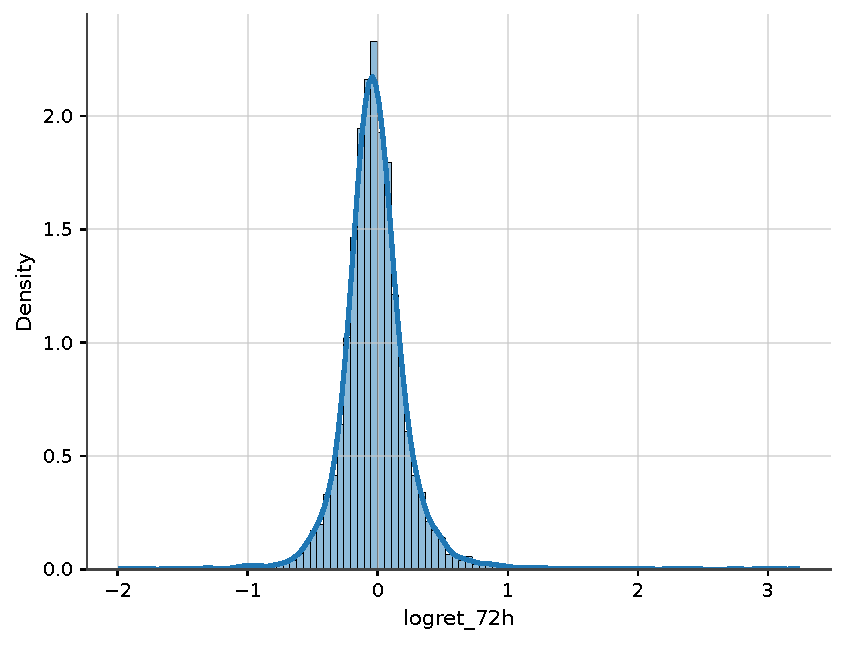
\includegraphics[width=0.65\linewidth,height=\textheight,keepaspectratio]{figures/final/fig-3-1.pdf}

}

\caption{\label{fig-return-dist}Distribution of the 72-hour log return
target variable, pooled across all tokens. The distribution exhibits a
sharp peak and significantly heavier tails than a comparable normal
distribution, justifying the use of quantile-based models.}

\end{figure}%

Furthermore, the properties of this distribution are not static.
Analysis of the underlying 12-hour returns reveals that the shape of the
distribution is highly conditional on the broader market environment. By
defining macro-regimes based on the quartiles of SOL's 12-hour return,
it becomes evident that the conditional distribution of token returns
shifts systematically. As shown in \textbf{Figure 4.2}, ``Bull'' regimes
are associated with positive skew and a fatter right tail, whereas
``Bear'' regimes exhibit heavier left tails, signalling increased
downside risk. This empirical finding of regime-dependence is critical,
as it justifies the need for a \emph{conditional} forecasting model that
can adapt its predicted quantiles based on contextual features.

\begin{figure}[H]

\centering{

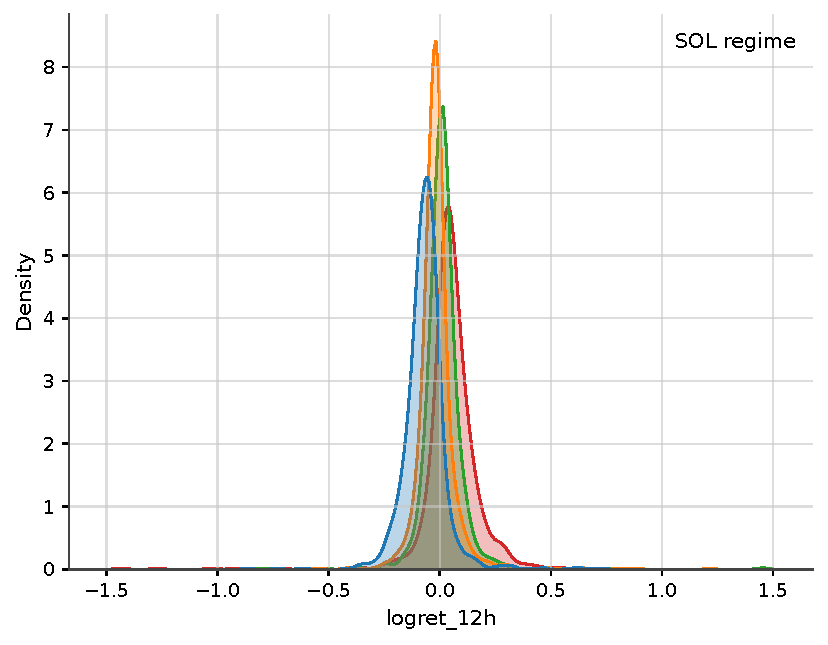
\includegraphics[width=0.7\linewidth,height=\textheight,keepaspectratio]{figures/final/fig-eda-regime-return-dist.pdf}

}

\caption{\label{fig-regime-dist}Conditional distribution of 12-hour
token returns, faceted by the SOL macro-regime. The shape, skew, and
tail behaviour of the returns change significantly depending on the
broader market context.}

\end{figure}%

Finally, it is important to note that this construction results in an
overlapping target variable. A new 72-hour forecast is generated every
12 hours, meaning that the forecast periods overlap significantly. This
has direct implications for the evaluation methodology, as the resulting
forecast errors will be serially correlated by construction. As detailed
in the literature review and methodology chapters, this requires the use
of specific techniques, such as blocked cross-validation and HAC-robust
statistical tests, to ensure valid inference.

\section{Data Preprocessing and
Cleaning}\label{data-preprocessing-and-cleaning}

The \textbf{cleaning strategy} proceeded in stages: (i) temporal
alignment to fixed 12-hour bins; (ii) gap detection and minimal
winsorisation; (iii) removal or flagging of structurally missing
segments; and (iv) post-aggregation QA checks. Implementation snippets
are referenced in the Appendix.

Before any features could be engineered, the raw, multi-source panel
dataset underwent a rigorous cleaning and preprocessing pipeline. This
was a critical phase designed to handle the significant data quality
challenges inherent in cryptocurrency markets, such as missing
observations and inconsistent token histories, ensuring the final
dataset was robust and suitable for modelling. The initial raw data
contained approximately \textbf{18\% missing values} in the core OHLCV
columns alone, with some on-chain features like \texttt{holder\_count}
missing nearly 40\% of their data (see Appendix 1, Table 3 for a full
breakdown).

The nature of this missingness was not uniform. As illustrated by the
heatmap in \textbf{Figure 4.3}, the data gaps were highly structured.
Some tokens (e.g., \texttt{MEW}, \texttt{ZEREBRO}) had clean data but
only after a late start date, while others exhibited intermittent,
patchy gaps throughout their history. This heterogeneity necessitated a
multi-step strategy rather than a single, one-size-fits-all approach.

\begin{figure}

\centering{

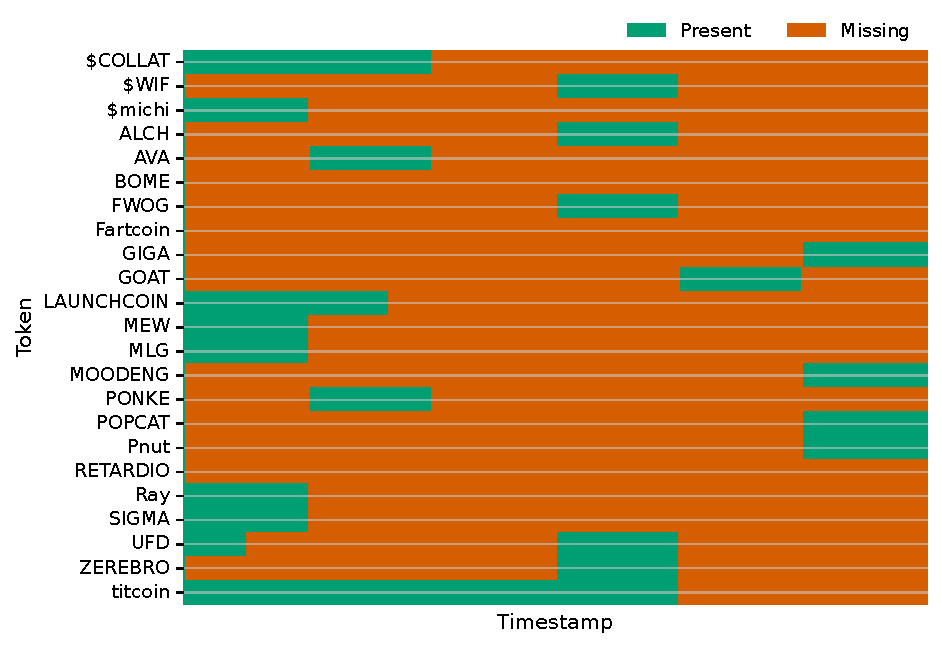
\includegraphics[width=0.85\linewidth,height=\textheight,keepaspectratio]{figures/final/fig-3-6-ohlcv-missingness-heatmap.pdf}

}

\caption{\label{fig-ohlcv-heat}Heatmap of OHLCV data presence across the
token universe over time (Green = Present, Red = Missing). The
block-like structure for some tokens indicates late listings, while
sporadic red patches show intermittent data gaps, motivating a hybrid
cleaning strategy.}

\end{figure}%

\subsubsection{Temporal Alignment and
Clipping}\label{temporal-alignment-and-clipping}

To ensure temporal consistency, each time series was first clipped to
begin only from its first fully valid OHLCV observation. This step,
detailed in the strategy summary in Appendix 1
\textbf{@sec-cleaning-strategy}, removes spurious data from pre-launch
or illiquid initial listing periods, which could otherwise contaminate
the analysis. Tokens with insufficient history after this clipping
process (e.g., \texttt{\$COLLAT}) were dropped from the universe
entirely.

\subsubsection{Imputation Strategy}\label{imputation-strategy}

A key challenge was to fill the remaining intermittent gaps without
distorting the underlying distributional properties of the data. Several
imputation methods were benchmarked on simulated missing data.
Counter-intuitively, the analysis revealed that a simple linear
interpolation outperformed more complex methods like Kalman smoothing in
terms of Root Mean Squared Error (RMSE) (see Appendix 1 Table 4
\textbf{@\#imp-table} for benchmark results). This finding suggests that
for small, sporadic gaps, a simple interpolation preserves the local
price trajectory and its inherent noise structure more effectively than
methods that impose stronger, potentially smoothing, structural
assumptions.

Therefore, the final strategy adopted was a hybrid approach: linear
interpolation to fill the majority of gaps, supplemented by a
forward-fill for a maximum of two consecutive 12-hour bars.

\section{Exploratory Data Analysis}\label{exploratory-data-analysis}

Following the preprocessing pipeline, an extensive exploratory data
analysis (EDA) was conducted to uncover the key empirical properties of
the data. This section presents the three most critical findings that
provide a direct, data-driven justification for the subsequent feature
engineering choices and the selection of a non-parametric, conditional
forecasting model. \emph{See Appendix 4 for full EDA figures, and
Appendix 5 code}

\subsubsection{Volatility Clustering and Asymmetric
Leverage}\label{volatility-clustering-and-asymmetric-leverage}

The data exhibits two foundational properties of financial time series
that invalidate simple, static risk models. First, strong volatility
clustering is evident in the autocorrelation of absolute 12-hour
returns, confirming that risk is time-varying and motivating the
inclusion of dynamic volatility features.

Second, the relationship between returns and subsequent volatility is
asymmetric. An analysis regressing 12-hour log returns against forward
36-hour realised volatility reveals a distinct U-shaped pattern, as
shown in \textbf{Figure 4.4}. This confirms that variance is conditional
on the magnitude of recent returns, with large moves in either direction
predicting elevated future volatility. The effect is slightly stronger
for negative returns, consistent with a ``crypto leverage effect'' where
downside shocks lead to greater market instability. This non-linear
dynamic necessitates a modelling approach, such as the Quantile
Regression Forest used in this study, that can naturally capture such
relationships and adapt its prediction interval widths based on the
direction and magnitude of recent price shocks.

\begin{figure}

\centering{

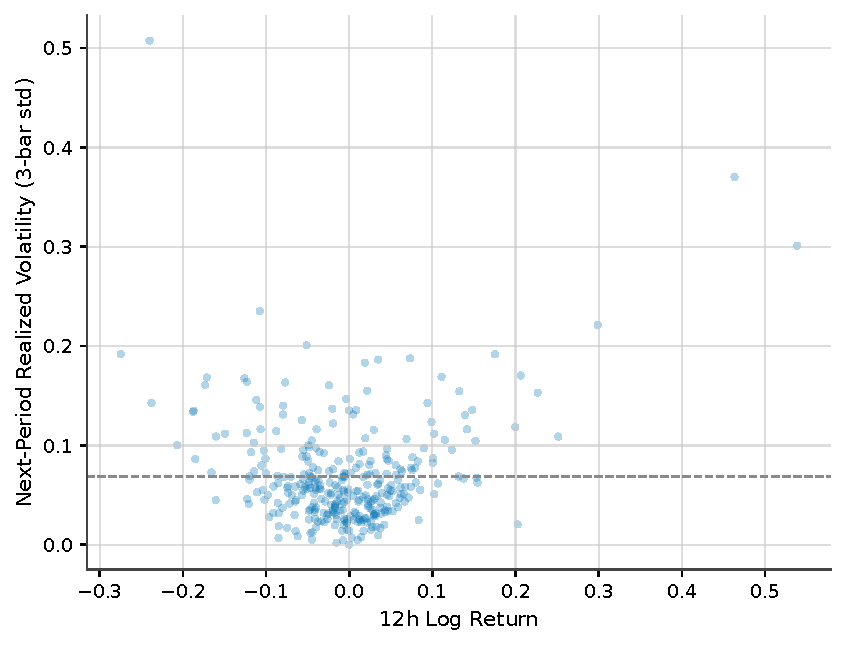
\includegraphics[width=0.65\linewidth,height=\textheight,keepaspectratio]{figures/final/fig-eda-return-vs-future-vol.pdf}

}

\caption{\label{fig-leverage-effect}A scatter plot of 12h Log Return
vs.~Next-Period Realised Volatility. The U-shaped pattern, with a
slightly steeper slope for negative returns, illustrates the asymmetric
leverage effect.}

\end{figure}%

\subsubsection{Feature Redundancy and
Collinearity}\label{feature-redundancy-and-collinearity}

An analysis of the correlation structure between 18 core features was
conducted to identify potential multicollinearity, which can destabilise
tree-based ensemble models. As shown in the Pearson correlation matrix
in \textbf{Figure 3.5}, several feature pairs exhibit extremely high
linear relationships. The most significant correlations were observed
between:

\begin{itemize}
\tightlist
\item
  \texttt{token\_close\_usd} and \texttt{token\_volume\_usd}
  (\(r \\approx 0.999\))
\item
  \texttt{btc\_close\_usd} and \texttt{tvl\_usd} (\(r \\approx 0.94\))
\item
  \texttt{sol\_close\_usd} and \texttt{tvl\_usd} (\(r \\approx 0.89\))
\end{itemize}

This finding is critical. It implies that highly collinear inputs can
inflate variance, degrade interpretability, and reduce generalisation;
we therefore prioritise redundancy control (filtering/aggregation)
during feature engineering and in later pruning. While these raw fields
were retained for the initial feature engineering phase to allow for the
construction of richer indicators (e.g., from OHLC data), this analysis
motivates the necessity of a subsequent feature pruning step. Reducing
this high level of collinearity before modelling is essential for
improving the stability, training speed, and interpretability of the
final Quantile Regression Forest.

\begin{figure}

\centering{

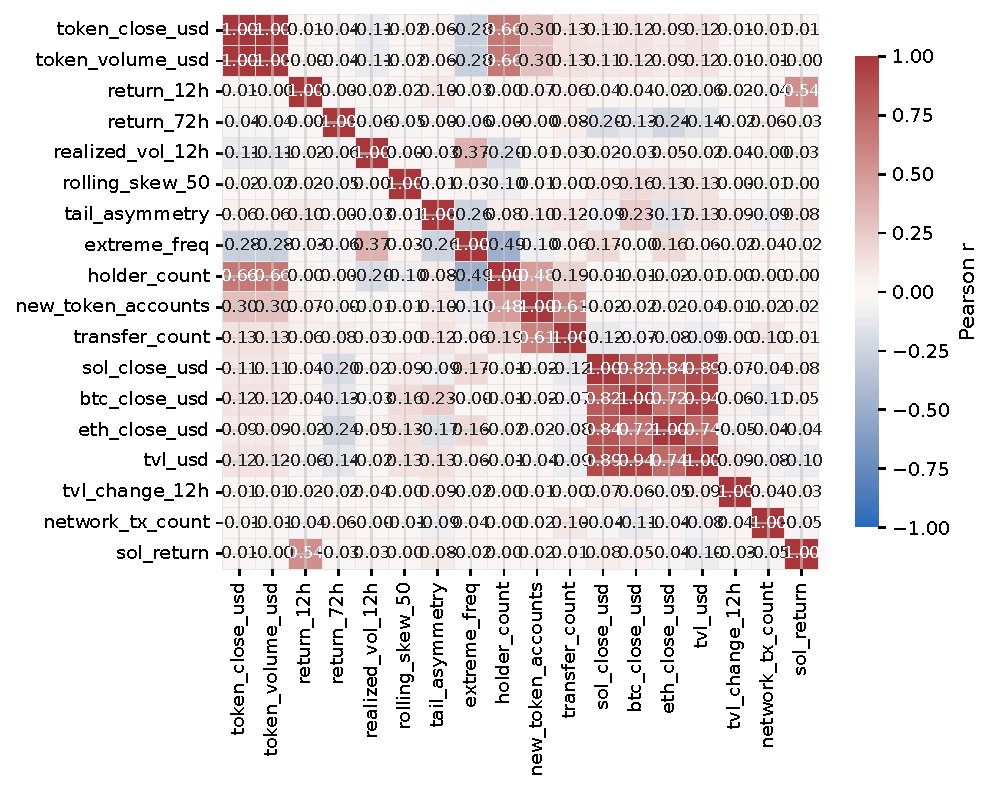
\includegraphics[width=1\linewidth,height=\textheight,keepaspectratio]{figures/final/fig-eda-pearson-corr.pdf}

}

\caption{\label{fig-leverage-effect}Pearson correlation matrix of key
features. The strong red blocks highlight pairs of highly correlated
variables, necessitating a feature pruning or aggregation strategy.}

\end{figure}%

\subsubsection{The Empirical Failure of Gaussian
Assumptions}\label{the-empirical-failure-of-gaussian-assumptions}

To provide a definitive, data-driven justification for model selection,
a baseline experiment was conducted to compare a naive Gaussian interval
forecast (defined as \(\\pm z \\cdot \\sigma\), using realised
volatility) against a simple Quantile Regression Forest. The results,
shown in \textbf{Figure 3.6}, are stark.

The naive Gaussian intervals systematically under-cover the true
outcomes across all nominal levels; for example, a nominal 80\% interval
achieves only \textasciitilde70\% empirical coverage. In contrast, even
a basic QRF model tracks the ideal 45-degree line far more closely,
demonstrating superior calibration by adapting to the true fat-tailed
and skewed nature of the returns.

Crucially, this improvement in calibration does not come at the cost of
precision. At a nominal 80\% coverage level, the QRF intervals were also
significantly sharper, with an average width of 0.1682 compared to
0.2038 for the naive method. This dual failure of the Gaussian
approach---in both calibration and sharpness---provides the ultimate
empirical justification for rejecting simple parametric assumptions and
adopting a non-parametric methodology like QRF for this dataset.

\begin{figure}

\centering{

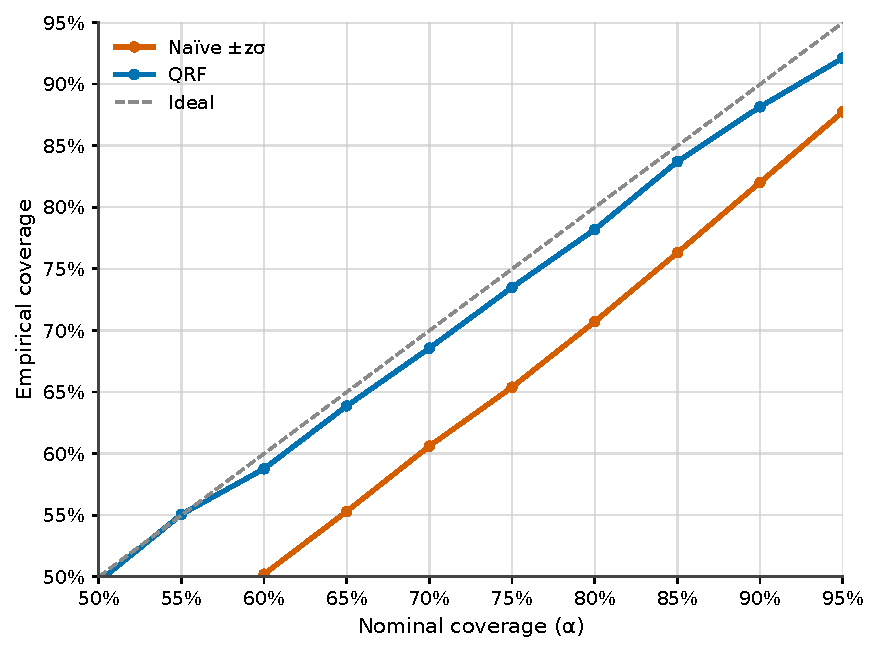
\includegraphics[width=0.65\linewidth,height=\textheight,keepaspectratio]{figures/final/fig-eda-calibration-comparison.pdf}

}

\caption{\label{fig-calibration-curve}Calibration curve comparing the
empirical vs.~nominal coverage of naive Gaussian intervals and QRF
intervals. The QRF's proximity to the ideal line demonstrates its
superior ability to model the data's true distribution.}

\end{figure}%

\emph{Implementation note:} plotting and calibration code is provided in
the Appendix, alongside other experimental figures.

\section{Feature Engineering and
Selection}\label{feature-engineering-and-selection}

Following the data preparation and exploratory analysis, an extensive
feature set was engineered. This process was guided by two main
principles: first, all predictors must be strictly causal, using only
information available at or before time \(t\); second, the feature set
should be designed to capture the specific statistical properties---such
as volatility clustering, asymmetry, and regime-dependence---identified
in the EDA.

\subsubsection{Feature Construction by
Family}\label{feature-construction-by-family}

A complete feature dictionary with raw feature definitions,
transformations, and data sources is provided in the Appendix 1; this
section summarises the construction logic by family.

The engineered set focuses on signals that respond to the unique
dynamics of cryptocurrency markets. The literature supports using a
diverse set of technical and on-chain indicators, as machine learning
models can effectively synthesise these signals to improve predictive
accuracy (\citeproc{ref-Akyildirim2021}{Akyildirim, Goncu and Sensoy,
2021}). The constructed features fall into five families:

\begin{enumerate}
\def\labelenumi{\arabic{enumi}.}
\tightlist
\item
  \textbf{Momentum \& Trend:} Standard indicators such as 12h and 36h
  log-returns, the 14-period Relative Strength Index (RSI), and MACD
  were created to capture trend and mean-reversion dynamics.
\item
  \textbf{Volatility \& Tails:} To model the observed volatility
  clustering and leverage effects, features such as realised volatility
  over 3 and 6 bars, downside-only volatility, and the Average True
  Range (ATR) were included. Higher-moment estimators like rolling
  36-hour skewness were also engineered to capture tail asymmetry.
\item
  \textbf{Liquidity \& Flow:} The Amihud illiquidity measure and volume
  z-scores were constructed to provide the model with signals about
  market depth and trading frictions, which are conditions under which
  prediction intervals should widen.
\item
  \textbf{On-Chain Activity:} To capture fundamental network health,
  features such as the growth rate of unique wallets and the ratio of
  new accounts to total holders were included, consistent with the
  on-chain data availability constraints.
\item
  \textbf{Market Context:} To model the cross-asset spillovers
  identified in the literature, features such as the 12h returns for
  SOL, BTC, and ETH, as well as the rolling 36h correlation of each
  token to these majors, were created. This explicitly allows the model
  to learn a dynamic, implicit beta to the broader market.
\end{enumerate}

A complete feature dictionary, including formulas and window lengths, is
provided in Appendix 1.

\subsubsection{Redundancy Control and
Pruning}\label{redundancy-control-and-pruning}

The initial engineering process generated over 90 candidate features. To
create a final feature set that was both predictive and robust, a
systematic, three-stage pruning pipeline was implemented:

\begin{enumerate}
\def\labelenumi{\arabic{enumi}.}
\tightlist
\item
  \textbf{Initial Filtering:} Features with near-zero variance or
  excessive missingness (\textgreater80\%) were removed.
\item
  \textbf{Collinearity Filter:} To improve model stability, one feature
  from any pair with a Pearson correlation coefficient \(|\rho| > 0.98\)
  was removed.
\item
  \textbf{Gain-Based Pruning:} A computationally inexpensive LightGBM
  model was trained to predict the median (\(\tau=0.50\)) return. Any
  feature contributing less than 0.3\% to the total gain was pruned.
  This resulted in a core set of \textbf{29 predictors} that explained
  \textbf{99.3\%} of the model's total gain.
\end{enumerate}

The resulting feature set, designated \texttt{features\_v1}, was frozen
for all subsequent median-based modelling. A second set,
\texttt{features\_v1\_tail}, was created by reintroducing several
theoretically important but low-gain tail-risk indicators (e.g.,
\texttt{extreme\_count\_72h}) for use in the final quantile models. This
structured process ensures the models are built upon a rich, yet
parsimonious, set of predictors. \emph{The full code, summary write up
and feature gain table (table 6) can be found in Appendix 1}

\bookmarksetup{startatroot}

\chapter{Methods}\label{methods}

This chapter details the modelling and evaluation framework used to
forecast 72-hour log-returns for mid-cap Solana tokens. Building on last
section, we specify the conditional-quantile models, the leakage
controls, and the blocked walk-forward design under which all models are
trained and evaluated. All formulas, definitions and notations are
summarised in Appendix 2.

\emph{See Appendix 2 and the respective sections within Appendix 4
(Figures) and 5 (Code) for additional supporting content}

Our predictive target is the 72-hour log-return defined in the last
section. To avoid redundancy we refer to that definition and denote the
conditional quantile function at level \(\tau\) by \(q_\tau(x)\) and its
estimator by \(\widehat q_\tau(x)\). All models are trained per token
(no cross-sectional pooling) using only that token's own history. The
design matrix uses the pruned feature-set v1, with numeric columns
standardised on the Train slice only; categorical indicators are one-hot
encoded with an intercept.

\section{Rolling design, feature set, and leakage
controls}\label{sec-rolling}

\textbf{Blocked walk-forward.} For each token we use:

\begin{itemize}
\tightlist
\item
  \textbf{Train:} 120 bars (\textasciitilde60 days)\\
\item
  \textbf{Calibrate:} 24 bars (non-crossing + band calibration only)\\
\item
  \textbf{Test:} 6 bars (72 h)\\
\item
  \textbf{Step:} 6 bars (non-overlapping Test windows)
\end{itemize}

Features at time \(t\) use only information available by the close of
bar \(t\); the target is \(y_{t+6}\). We report both micro and macro
averages across tokens; precise formulas in Appendix 2.

\textbf{Feature set \& leakage controls.} We use feature-set v1 (29
predictors) grouped into momentum, volatility, liquidity/flow, on-chain
activity, and market context. Rolling statistics and lags are computed
with windows that end at \(t\); the design matrix at \(t\) excludes any
information from \(t{+}1…t{+}6\). \emph{The full feature dictionary can
be see in Appendix 2 (Table 4).}

\textbf{Global non-crossing \& calibration.} Base quantiles are made
monotone in \(\tau\) via row-wise isotonic rearrangement
(pool-adjacent-violators), then central bands are adjusted using
split-conformal prediction on the 24-bar calibration slice. Score
definitions and order-statistic inflation for the 80\% and 90\% bands
are given in Appendix 2.

\textbf{Software.} Library and environment details are listed in
Appendix 4.

\subsubsection{Model Building}\label{model-building}

We present a compact, self-contained statement of each model
(objective/estimator) in the main text, with derivations and
implementation details in Appendix 2. The core validation
metrics---pinball loss, reliability, and interval coverage/width, are
defined in the main text; the full DM--HAC with HLN specification
appears in Appendix 2. All figures are collected in Appendix 4, and all
applied code is provided in Appendix 5.

\section{Linear Quantile Regression Model
(Baseline)}\label{linear-quantile-regression-model-baseline}

\textbf{Estimator.} For each quantile \(\tau\) in the chosen set we fit
a linear quantile regression model using the Koenker--Bassett
formulation. In the rolling back‑test reported here the quantile grids
were \(\{0.05,0.25,0.50,0.75,0.95\}\) for the main baseline and
\(\{0.10,0.50,0.90\}\) for a simpler variant. For each \(\tau\) we solve

\[
\widehat\beta_\tau = \arg\min_{\beta\in\mathbb{R}^p} \sum_{t\in\text{Train}} \rho_\tau(y_t - \mathbf{x}_t^{\top}\beta), \quad \rho_\tau(u) = u\,(\tau-\mathbf{1}\{u<0\}),
\]

with no regularisation. The models are fitted with
\texttt{statsmodels.QuantReg}.

\textbf{Design matrix \& fitting.} We use the ``features\,v1'' data set.
Numeric predictors are scaled within each training window using a robust
scaler or standard scaler depending on the notebook; categorical
predictors (such as token identifier, momentum bucket, day of week,
etc.) are one‑hot encoded with the first level dropped. An intercept
term is added by \texttt{sm.add\_constant}. The pre‑processor is fit
only on the training slice and then applied to the calibration and test
slices.

\textbf{Non‑crossing.} In the variant with three quantiles, we apply a
simple post‑hoc non‑crossing adjustment so that the 10th‑percentile
predictions never exceed the median and the 90th‑percentile predictions
never fall below it. No isotonic rearrangement across a larger grid of
quantiles was used in these baselines.

\subsubsection{Reporting}\label{reporting}

We report \textbf{pinball loss} by \(\tau\), \textbf{reliability}
(empirical \(\widehat F_\tau\) vs nominal \(\tau\)),
\textbf{coverage/width} at 80\%/90\%, and \textbf{Diebold--Mariano}
tests vs.~LightGBM and QRF. See appendix 4 for varient analysis and
extra figures.

\subsubsection{Variants: LQR variants (pinball at key
quantiles)**}\label{tbl-lqr-variants}

\begin{longtable}[]{@{}
  >{\raggedright\arraybackslash}p{(\linewidth - 8\tabcolsep) * \real{0.1348}}
  >{\raggedright\arraybackslash}p{(\linewidth - 8\tabcolsep) * \real{0.2360}}
  >{\centering\arraybackslash}p{(\linewidth - 8\tabcolsep) * \real{0.1573}}
  >{\centering\arraybackslash}p{(\linewidth - 8\tabcolsep) * \real{0.1461}}
  >{\raggedright\arraybackslash}p{(\linewidth - 8\tabcolsep) * \real{0.3258}}@{}}
\toprule\noalign{}
\begin{minipage}[b]{\linewidth}\raggedright
Variant
\end{minipage} & \begin{minipage}[b]{\linewidth}\raggedright
Estimator
\end{minipage} & \begin{minipage}[b]{\linewidth}\centering
Non-crossing
\end{minipage} & \begin{minipage}[b]{\linewidth}\centering
Calibration
\end{minipage} & \begin{minipage}[b]{\linewidth}\raggedright
Pinball (τ=.10 / .50 / .90)
\end{minipage} \\
\midrule\noalign{}
\endhead
\bottomrule\noalign{}
\endlastfoot
\textbf{LQR v1} & statsmodels QuantReg & ✗ & ✗ & --- / \textbf{8.0238} /
--- \\
\textbf{LQR v2} & statsmodels QuantReg & ✓* & ✗ & \textbf{0.0400} /
\textbf{0.0640} / \textbf{0.3850} \\
\end{longtable}

\textbf{Why this baseline.} LQR provides a transparent parametric
benchmark. In heavy-tailed, skewed crypto returns, its characteristic
tail mis-calibration (see \texttt{@fig-lqr-calibration} in Appendix 2)
motivates the flexible, non-parametric models.

\section{Gradient-boosted trees with quantile loss (LightGBM
baseline)}\label{sec-lgbm}

\textbf{Estimator (pinball objective).} For each quantile \(\tau\), we
fit a gradient-boosted tree model that minimizes the pinball loss. At
boosting step \(m\), the predictor updates as
\(F^{(\tau)}_{m}(x) = F^{(\tau)}_{m-1}(x) + \eta\,f^{(\tau)}_{m}(x)\),
where the regression tree \(f^{(\tau)}_{m}\) is trained on
pseudo-residuals
\(g^{(\tau)}_{t} = \tau - \mathbf{1}\{y_t < F^{(\tau)}_{m-1}(x_t)\}\).

\textbf{Design matrix and tuning.} In the v1 baseline, we pass numeric
features unchanged and one-hot encode categorical variables via a
\texttt{ColumnTransformer}. We fix hyperparameters
(\texttt{n\_estimators=500}, \texttt{learning\_rate=0.05},
\texttt{subsample=0.9}, \texttt{colsample\_bytree=0.9},
\texttt{min\_child\_samples=20}) and fit models for
\(\tau\in\{0.05,0.25,0.50,0.75,0.95\}\). In v2, we tune hyperparameters
per quantile with Optuna over \texttt{num\_leaves}, \texttt{max\_depth},
\texttt{min\_data\_in\_leaf}, \texttt{learning\_rate}, and sampling
fractions; categorical features are cast to pandas \texttt{Categorical}
so LightGBM handles them natively. In later variants (v3/v4), we re-fit
with the v2-selected settings, deepen trees (e.g.,
\texttt{max\_depth=10}), and enable early stopping.

\textbf{Calibration and non-crossing.} We apply conformal quantile
regression to all LightGBM variants. v1--v2 use \textbf{split-conformal}
adjustments (one-sided shifts of lower/upper quantiles). v3--v4 use
\textbf{CV-plus} (two-sided) calibration with residual winsorization,
and we exclude calibration rows with high imputation fractions. We do
not apply isotonic rearrangement; non-crossing is therefore not enforced
explicitly.

\textbf{Reporting.} For each \(\tau\), we report pinball loss; for
intervals, we report empirical coverage and mean half-width of the 80\%
prediction interval. v3 additionally includes Diebold--Mariano tests for
model comparisons.

\subsubsection{Variants}\label{variants}

\begin{longtable}[]{@{}
  >{\raggedright\arraybackslash}p{(\linewidth - 8\tabcolsep) * \real{0.1538}}
  >{\raggedright\arraybackslash}p{(\linewidth - 8\tabcolsep) * \real{0.1154}}
  >{\raggedright\arraybackslash}p{(\linewidth - 8\tabcolsep) * \real{0.2308}}
  >{\raggedright\arraybackslash}p{(\linewidth - 8\tabcolsep) * \real{0.4038}}
  >{\raggedleft\arraybackslash}p{(\linewidth - 8\tabcolsep) * \real{0.0962}}@{}}
\toprule\noalign{}
\begin{minipage}[b]{\linewidth}\raggedright
Variant
\end{minipage} & \begin{minipage}[b]{\linewidth}\raggedright
Tuning
\end{minipage} & \begin{minipage}[b]{\linewidth}\raggedright
Calibration
\end{minipage} & \begin{minipage}[b]{\linewidth}\raggedright
Pinball (key τ)
\end{minipage} & \begin{minipage}[b]{\linewidth}\raggedleft
Cov. 80\%
\end{minipage} \\
\midrule\noalign{}
\endhead
\bottomrule\noalign{}
\endlastfoot
\textbf{v1 (base)} & Fixed & Split-conformal & ≈ 0.0359 (@.05), 0.0659
(@.50), 0.0601 (@.95) & n/a \\
\textbf{v2 (tuned)} & Optuna per τ & Split-conformal & ≈ 0.0553 (@.10),
0.0656 (@.50), 0.0778 (@.90) & ≈97.5\% \\
\textbf{v4 (final)} & v2 params + ES & CV-plus, winsorised & ≈ 0.0316
(@.10), 0.0473 (@.25), 0.0755 (@.75) & ≈82.9\% \\
\end{longtable}

\textbf{Why this baseline.} Quantile LightGBM is a strong, non-linear
comparator that is fast, interaction-aware, and---after
split-conformalisation---near-nominal in coverage with comparatively
tight bands, setting a demanding reference for QRF (§4.4).

\section{Quantile Regression Forests (core model)}\label{sec-qrf}

\textbf{Estimator.} For each query point \(x\), we fit a Quantile
Regression Forest (QRF) as an ensemble of regression trees and define
observation weights \(w_t(x)\) over training responses \(y_t\) that
share terminal nodes with \(x\). The conditional distribution
\(\hat F_x(\cdot)\) is the empirical CDF of these weighted responses,
and the \(\tau\)-level quantile is

\[
\hat q_\tau(x)\;=\;\inf\Bigl\{q:\;\sum_{t\in\text{train}} w_t(x)\,\mathbf{1}\{y_t\le q\}\ge \tau\Bigr\}.
\]

\textbf{Time-decay weighting.} To emphasize recent information, we apply
exponentially decaying sample weights with half-life \(h=60\) bars. If
\(\Delta t\) denotes the age (in 12-hour bars) of observation \(t\), we
set \(\omega_t \propto 2^{-\Delta t/h}\) and normalize so that
\(\sum_t \omega_t=1\). These \(\omega_t\) are supplied to the forest via
\texttt{sample\_weight}.

\textbf{Preprocessing and tuning.} Categorical predictors
(\texttt{token}, \texttt{momentum\_bucket}, \texttt{day\_of\_week},
\texttt{tail\_asym}, \texttt{extreme\_flag1}, \texttt{vol\_regime}) are
one-hot encoded; numerical predictors are standardized. A single Optuna
study searches over the number of trees, maximum depth, minimum samples
per leaf, and feature subsampling to minimize average pinball loss
across quantiles and rolling folds. The tuned specification typically
selects \(\sim\!1050\) trees with relatively deep depth and small leaf
size.

\textbf{Calibration and non-crossing.} Raw QRF quantiles can cross and
often over-cover. We therefore apply:

\begin{enumerate}
\def\labelenumi{\arabic{enumi}.}
\tightlist
\item
  \textbf{Isotonic regression.} After predicting
  \(\{q_{\tau_i}(x)\}_{i=1}^m\), we fit a one-dimensional isotonic
  regression along the quantile axis to enforce monotonicity, which
  preserves spacing better than simple sorting.
\item
  \textbf{Regime-aware residual quantile calibration.} For each rolling
  window, we compute residuals on a 24-bar calibration slice, winsorize
  them, stratify by a volatility-regime indicator
  (\texttt{vol\_regime}), and estimate separate residual quantiles for
  ``quiet'' and ``volatile'' periods. Lower/upper quantiles (e.g., 0.10
  and 0.90) are adjusted by the appropriate residual quantile; a
  median-bias correction is applied at \(\tau=0.50\). Calibration rows
  with \textgreater30\% imputed features are excluded.
\item
  \textbf{Split-conformal top-up.} To obtain two-sided \((1-\alpha)\)
  prediction intervals (e.g., 80\% and 90\%), we use split-conformal
  adjustments: we add the \(\lceil (n+1)\alpha\rceil\)-th largest
  positive residual to the upper bound and subtract the corresponding
  negative residual from the lower bound, yielding finite-sample,
  distribution-free coverage.
\end{enumerate}

\textbf{Reporting and variants.} We evaluate via rolling-window
cross-validation (train 120 bars, calibrate 24, test 6). We report
per-quantile pinball loss, empirical coverage, and average interval
width, and use Diebold--Mariano tests to compare QRF with linear QR and
LightGBM.

\begin{longtable}[]{@{}
  >{\raggedright\arraybackslash}p{(\linewidth - 12\tabcolsep) * \real{0.1728}}
  >{\centering\arraybackslash}p{(\linewidth - 12\tabcolsep) * \real{0.0741}}
  >{\centering\arraybackslash}p{(\linewidth - 12\tabcolsep) * \real{0.0864}}
  >{\raggedright\arraybackslash}p{(\linewidth - 12\tabcolsep) * \real{0.3704}}
  >{\raggedleft\arraybackslash}p{(\linewidth - 12\tabcolsep) * \real{0.0988}}
  >{\raggedleft\arraybackslash}p{(\linewidth - 12\tabcolsep) * \real{0.0988}}
  >{\raggedleft\arraybackslash}p{(\linewidth - 12\tabcolsep) * \real{0.0988}}@{}}
\toprule\noalign{}
\begin{minipage}[b]{\linewidth}\raggedright
Variant
\end{minipage} & \begin{minipage}[b]{\linewidth}\centering
Time-decay
\end{minipage} & \begin{minipage}[b]{\linewidth}\centering
Non-crossing
\end{minipage} & \begin{minipage}[b]{\linewidth}\raggedright
Calibration
\end{minipage} & \begin{minipage}[b]{\linewidth}\raggedleft
τ=0.10 pinball
\end{minipage} & \begin{minipage}[b]{\linewidth}\raggedleft
τ=0.50 pinball
\end{minipage} & \begin{minipage}[b]{\linewidth}\raggedleft
τ=0.90 pinball
\end{minipage} \\
\midrule\noalign{}
\endhead
\bottomrule\noalign{}
\endlastfoot
\textbf{QRF-v1 (base)} & ✗ & sort & none & 0.0286 & 0.0725 & 0.0682 \\
\textbf{QRF-v2 (CQR + regime)} & ✓ & isotonic & regime-aware residual
quantile + split-conformal & 0.0224 & 0.0610 & 0.0660 \\
\textbf{QRF-v3 (tuned)} & ✓ & isotonic & same as v2 & ≈ 0.0229 & ≈
0.0653 & ≈ 0.0670 \\
\textbf{QRF-v4 (final)} & ✓ & isotonic & regime-aware residual quantile
+ split-conformal (CV-plus) & 0.0224 & 0.0610 & 0.0660 \\
\end{longtable}

\textbf{Final specification and rationale.} We adopt the tuned,
time-decay QRF (v4) as the core model. It combines (i) isotonic
enforcement across quantiles, (ii) regime-aware residual quantile
offsets with winsorization and exclusion of heavily imputed rows, and
(iii) a small split-conformal top-up to achieve nominal coverage. This
preserves per-quantile reliability and yields central intervals that are
sharper than the LightGBM baseline (see §5): pinball loss at
\(\tau\in\{0.10,0.90\}\) is \textasciitilde0.022 and 0.066, and the
median-level loss (\textasciitilde0.061) matches the boosted baseline.

\textbf{All model-variant figures and additional analyses are provided
in Appendix 4 (Extras).}

\section{Validation, metrics, and statistical
tests}\label{validation-metrics-and-statistical-tests}

This section formalises the criteria used to compare models. Definitions
are in Appendix 2.

\subsubsection{Losses and calibration
metrics}\label{losses-and-calibration-metrics}

\textbf{Pinball loss.} Primary score for each \(\tau\); we report
per-\(\tau\) means (with dispersion across tokens/folds) and a composite
average over \(\mathcal T=\{0.05,0.10,0.25,0.50,0.75,0.90,0.95\}\).

\textbf{Empirical coverage \& average width.} For central \((1-\alpha)\)
bands (after non-crossing and calibration) we report coverage, average
width, and \textbf{coverage error}
\(|\widehat{\mathrm{cov}}-(1-\alpha)|\). We also examine
\textbf{conditional coverage} by deciles of predicted width.

\textbf{Quantile reliability / calibration curves.} We plot empirical
hit-rates \(\widehat F_\tau\) against nominal \(\tau\); the ideal line
is 45°.

\textbf{Proper scoring rule.} We include the \textbf{interval score}
(Gneiting--Raftery, 2007) for completeness; CRPS links are noted in the
appendix.

\emph{See Appendix 2 table 3 for definitions}

\subsubsection{Statistical comparisons}\label{statistical-comparisons}

Pairwise comparisons use \textbf{Diebold--Mariano} tests on pinball-loss
differentials with \textbf{Newey--West} HAC variance and the
\textbf{Harvey--Leybourne--Newbold} small-sample correction.
((\citeproc{ref-Harvey1997}{Harvey, Leybourne and Newbold, 1997};
\citeproc{ref-newey1987}{\textbf{newey1987?}}))

We further build on this test using the \textbf{Model Confidence Set} by
(\citeproc{ref-hansen2011}{\textbf{hansen2011?}}). \emph{See Appendix 2
table 3 for definitions}

\subsubsection{Additional analyses: regimes, conditional coverage, and
efficiency}\label{additional-analyses-regimes-conditional-coverage-and-efficiency}

The global scores above average over heterogeneous market states and
tokens. To better understand the adaptivity and economic value of
interval forecasts, we perform several sliced analyses on the Test
forecasts:

\begin{itemize}
\item
  \textbf{Regime analysis.} We stratify Test observations into
  \textbf{quiet}, \textbf{mid}, and \textbf{volatile} windows based on
  realised-volatility terciles. Within each regime we recompute
  empirical coverage, mean width, and reliability curves. This assesses
  whether models widen bands appropriately in turbulent markets and is
  visualised by regime-specific calibration curves (see Results Fig.
  \texttt{@fig-reliability-regime}).
\item
  \textbf{Conditional coverage by predicted width.} For each model and
  central interval, we sort forecasts into deciles of predicted band
  width. We then compute hit-rates within each decile to test whether
  wider intervals indeed cover more outcomes. A monotonically increasing
  hit-rate confirms that the model's widths are informative about
  uncertainty. The decile table and associated plot are reported in the
  Results (Fig. \texttt{@fig-cond-cov-width}; Table
  \texttt{@tbl-condcov-width}).
\item
  \textbf{Sharpness--coverage efficiency.} We summarise each
  model--interval pair by its average width and empirical coverage and
  display points on the efficiency plane (coverage on the y-axis, width
  on the x-axis). Points closer to the upper-left (high coverage and low
  width) are preferred. See Results (Fig.
  \texttt{@fig-efficiency-scatter}; Table
  \texttt{@tbl-efficiency-summary}) for the scatter and summary.
\end{itemize}

These additional analyses complement the global averages by revealing
regime-dependent behaviour, the information content of predicted widths,
and the sharpness--coverage trade-off.

\subsubsection{Robustness tests and
ablations}\label{robustness-tests-and-ablations}

We assess stability via \textbf{component-wise ablations} of the final
QRF:

\begin{itemize}
\tightlist
\item
  \textbf{Decay weights (ON/OFF).} Remove exponential time-decay
  (baseline half-life 60 bars).
\item
  \textbf{Calibration wrapper.} Replace residual-quantile offsets +
  split-conformal with pure split-conformal.
\item
  \textbf{Monotone rearrangement.} Disable isotonic non-crossing.
\item
  \textbf{Half-life sensitivity.} Test 30 and 90 bars around the
  baseline.
\item
  \textbf{Calibration scope.} Compute residual offsets per token (final)
  vs pooled.
\end{itemize}

For each toggle we report deltas in mean pinball, coverage (80\%/90\%),
and width relative to QRF-final, with HAC-adjusted DM tests for
significance.

\subsubsection{Cross-sectional heterogeneity and per-token
diagnostics}\label{cross-sectional-heterogeneity-and-per-token-diagnostics}

To avoid dominance by long or high-volume series, we summarise per-token
pinball, coverage, and width across all Test windows, show their
dispersion (boxplots), and include representative fan charts (q05--q95)
illustrating adaptivity. See Results Fig.
\texttt{@fig-pinball-by-token}, \texttt{@fig-fan-mlg},
\texttt{@fig-fan-ava}.

\section{Application: interval-aware
sizing}\label{application-interval-aware-sizing}

We outline a position-sizing rule that scales exposure inversely with
predicted interval width, subject to risk limits; implementation and
back-test appear in Results.

\bookmarksetup{startatroot}

\chapter{Results}\label{results}

\textbf{Experimental setup}

We evaluate LQR, LightGBM-Quantile, and QRF, across the τ-grid
\(\{0.05,0.10,0.25,0.50,0.75,0.90,0.95\}\). Unless noted otherwise,
results are \textbf{micro-averaged} across all test observations (with
macro averages by token in parentheses).

\emph{Appendix 3 contains the main supporting figures and tables for
this report section. For the full set of model analysis, cross model
comparison and more, see Appendix 4. See Appendix 5 for all validation
and statistical tests code.}

\section{Overall accuracy and
Calibration}\label{overall-accuracy-and-calibration}

Across the pooled rolling evaluation, QRF delivers the lowest mean
pinball loss at the left tail and lower-middle quantiles
\textbf{(\(\tau\) ∈ \{0.05, 0.10, 0.25\})}, remains competitive around
the median, and tracks the upper tails closely. LightGBM is generally
less accurate (higher pinball) but attains high coverage by producing
wider intervals. LQR is competitive near the centre and upper quantiles
but systematically under-covers (0.51 at 80\%). In terms of calibration,
QRF's 90\% bands are close to nominal (≈0.88), while 80\% bands remain
modestly under-covered (≈0.77). LightGBM over-covers (0.98 at 90\%),
consistent with conservative widths. These patterns hold at both the
pooled (micro) level and when averaging per token (macro).

\textbf{Pinball accuracy by quantile}

This Table reports the \textbf{mean pinball loss by tau and model}
(standard errors in parentheses; micro and macro reported). The main
findings are:

\begin{longtable}[]{@{}llll@{}}
\toprule\noalign{}
τ & LQR & LightGBM & QRF \\
\midrule\noalign{}
\endhead
\bottomrule\noalign{}
\endlastfoot
0.05 & 0.03015 & 0.03514 & \textbf{0.01406} \\
0.10 & 0.04094 & 0.03108 & \textbf{0.02244} \\
0.25 & 0.05524 & 0.04556 & \textbf{0.04159} \\
0.50 & 0.06302 & 0.06581 & \textbf{0.06103} \\
0.75 & \textbf{0.05539} & 0.07374 & 0.07162 \\
0.90 & \textbf{0.03707} & 0.06622 & 0.06597 \\
0.95 & \textbf{0.02399} & 0.05957 & 0.04783 \\
\end{longtable}

\emph{See Figure~\ref{fig-pinball-by-quantile-by-model} for the visual
representation.}

\begin{itemize}
\tightlist
\item
  \textbf{Lower tail (\(\tau\) = 0.05, 0.10):} QRF attains the lowest
  loss, with a sizable margin over LightGBM and a clear advantage over
  LQR. This indicates superior tail sensitivity --- crucial in
  heavy-tailed return series.
\item
  \textbf{Lower-middle (\(\tau\) = 0.25):} QRF remains best. This is the
  region where models often drift if lower-tail calibration is
  imperfect; the improvement reflects the corrected residual-offset rule
  (see below).
\item
  \textbf{Centre/upper (\(\tau\) = 0.50, 0.75, 0.90, 0.95):} LQR is
  competitive to slightly better at the strict median and some upper τ
  on pinball (a linear model can approximate the median well on smoothed
  features), but QRF is close and often within the standard error;
  LightGBM has the largest loss.
\item
  The \textbf{rank ordering} corresponds to the bar chart in Fig.
  Figure~\ref{fig-qrf-v3-reliability-global} (QRF's line adheres tightly
  to the 45° band except for a mild 80\% under-coverage discussed below)
  and your pinball bar plot (QRF best at 0.05--0.25; LQR competitive
  around 0.50--0.95; LightGBM worst across \(\tau\)).
\end{itemize}

\emph{The other models coverage can be see here: LQR V1
Figure~\ref{fig-lqr-calibration} , LightGBM
Figure~\ref{fig-lgbm-v4-calibration}}

QRF's non-parametric trees capture non-linear interactions that matter
most in the tails and asymmetric regimes; LQR's linear structure can
excel near the centre when the conditional median depends smoothly on
features. LightGBM's comparatively higher pinball reflects a tendency to
produce over-conservative intervals after calibration.

\textbf{Global calibration and reliability}

Figure Figure~\ref{fig-qrf-v3-reliability-global} plots the reliability
curve --- the empirical hit-rate \(\Pr\{y\le \hat q_\tau\}\) against the
nominal \(\tau\) with Wilson 95\% CIs. After correcting the
residual-offset rule (now using \(\delta_\tau = Q_\tau(r_\tau)\), not
\(Q_{1-\tau}\), for residuals \(r_\tau = y - \hat q_\tau\)), the QRF
curve lies close to the 45° line across the grid, with only a modest dip
around \(\tau\approx0.8\) that mirrors the slightly low 80\% interval
coverage (below).

\textbf{Coverage and width (pooled)} Table~\ref{tbl-cov-width}
summarises pooled coverage at 80\% and 90\% together with coverage error
(actual − target). QRF attains near-nominal 90\% coverage and slightly
low 80\% coverage; LightGBM over-covers, and LQR under-covers markedly.

\begin{longtable}[]{@{}llrr@{}}
\caption{Coverage and sharpness at central 80\% and 90\% intervals
(pooled).}\label{tbl-cov-width}\tabularnewline
\toprule\noalign{}
Interval & Model & Coverage & Coverage − target (Error) \\
\midrule\noalign{}
\endfirsthead
\toprule\noalign{}
Interval & Model & Coverage & Coverage − target (Error) \\
\midrule\noalign{}
\endhead
\bottomrule\noalign{}
\endlastfoot
80\% & LQR & 0.508163 & −0.291837 \\
80\% & LightGBM & 0.790362 & −0.009638 \\
80\% & QRF & 0.766421 & −0.033579 \\
90\% & LQR & 0.621769 & −0.278231 \\
90\% & LightGBM & 0.979435 & +0.079435 \\
90\% & QRF & 0.878146 & −0.021854 \\
\end{longtable}

\emph{See Figure~\ref{fig-coverage-by-model} for the visual
representation.}

\textbf{Key takeaways.}

\begin{itemize}
\tightlist
\item
  \textbf{QRF:} \(0.76\!\!-\!0.78\) at 80\% (error \(\approx\) −2--4
  p.p.); \(0.87\!\!-\!0.89\) at 90\% (error \(\approx\) −1--3 p.p.).
\item
  \textbf{LightGBM:} \(0.79\!\!-\!0.80\) at 80\%; \(0.98\!\!-\!0.99\) at
  90\% (+8--9 p.p. over-coverage), consistent with conservative widths.
\item
  \textbf{LQR:} \(0.51\) at 80\% and \(0.62\) at 90\% (−29 p.p. and −28
  p.p.), indicating intervals that are too narrow.
\end{itemize}

\textbf{?@fig-widths} shows the width distributions for the 80\% and
90\% intervals. For a given empirical coverage, QRF's bands are
materially tighter than LightGBM's (shorter right tails), reflecting a
better sharpness--coverage trade-off. (A model-level efficiency
scatter---coverage vs mean width---appears)

\textbf{State dependence (quiet / mid / volatile)}

Slicing by a rolling volatility regime
(Figure~\ref{fig-qrf-reliability-by-regime-bars}) shows coverage is
stable across regimes after the offset fix: \textasciitilde0.75--0.78
(80\%) and \textasciitilde0.87--0.88 (90\%) in quiet, mid, and volatile
windows. What varies is sharpness: widths scale strongly with regime
(quiet \textless{} mid ≪ volatile). In our pooled sample, the 90\% mean
width is *0.23--0.34 in quiet/mid versus \textasciitilde1.35 in volatile
periods, indicating that QRF widens bands adaptively to preserve
coverage rather than letting it collapse in turbulent markets.
LightGBM's over-coverage is uniform across regimes; LQR under-covers
everywhere.

\textbf{Practical significance}

\begin{enumerate}
\def\labelenumi{\arabic{enumi}.}
\tightlist
\item
  \textbf{Decision-useful tails.} QRF's lowest pinball at
  \(\tau\in\{0.05,0.10\}\) yields more reliable downside bounds (a
  forward-looking VaR analogue) while keeping the 90\% band near
  nominal, supporting position sizing, stop placement, and risk
  budgeting.
\item
  \textbf{Sharper bands at like-for-like coverage.} Relative to
  LightGBM, QRF achieves similar/better coverage with narrower
  intervals, improving capital efficiency for risk-aware sizing.
\item
  \textbf{Limits of linearity.} LQR's competitive median does not
  translate into calibrated intervals; systematic under-coverage at both
  80\% and 90\% confirms linear structure misses asymmetric tail
  behaviour in crypto returns.
\end{enumerate}

\section{Significance Testing}\label{significance-testing}

This subsection reports pairwise Diebold--Mariano (DM) tests on
pinball-loss differentials and the Model Confidence Set (MCS). Methods
(HAC-NW, small-sample correction, FDR at \(q\le 0.10\)) are specified in
appendix 3; here we focus on the outcomes.

\textbf{Pairwise significance (DM): where QRF wins}

QRF achieves systematic and statistically reliable gains over LightGBM
at the quantiles that define interval bands, and is competitive with LQR
elsewhere. Tokens with significant DM in favour of QRF (BH
\(q\le 0.10\)):

\begin{itemize}
\item
  \textbf{Lower tail} -- \textbf{\(\tau=0.10\):} QRF beats LightGBM on
  10/19 tokens (53\%); vs LQR 6/19 (32\%). -- \textbf{\(\tau=0.25\):}
  QRF beats LightGBM on 12/19 (63\%); vs LQR 7/19 (37\%).
\item
  \textbf{Centre} -- \textbf{\(\tau=0.50\):} Differences are small and
  seldom significant (QRF wins 7/19 (37\%) vs LightGBM; 5/19 (26\%) vs
  LQR).
\item
  \textbf{Upper tail} -- \textbf{\(\tau=0.95\):} Very strong advantage
  over LightGBM (16/19 tokens, 84\%); vs LQR 4/19 (21\%). --
  \textbf{\(\tau=0.90\):} Mixed/rare significance (5/19 against each
  comparator). -- \textbf{\(\tau=0.75\):} Mixed (6/19 depending on
  comparator).
\end{itemize}

These results highlight LightGBM's conservative, wider bands tend to
inflate pinball loss at the tails, where QRF maintains near-nominal
coverage with sharper intervals. Around the median, all models are
close, so statistical ties are expected.

\begin{center}
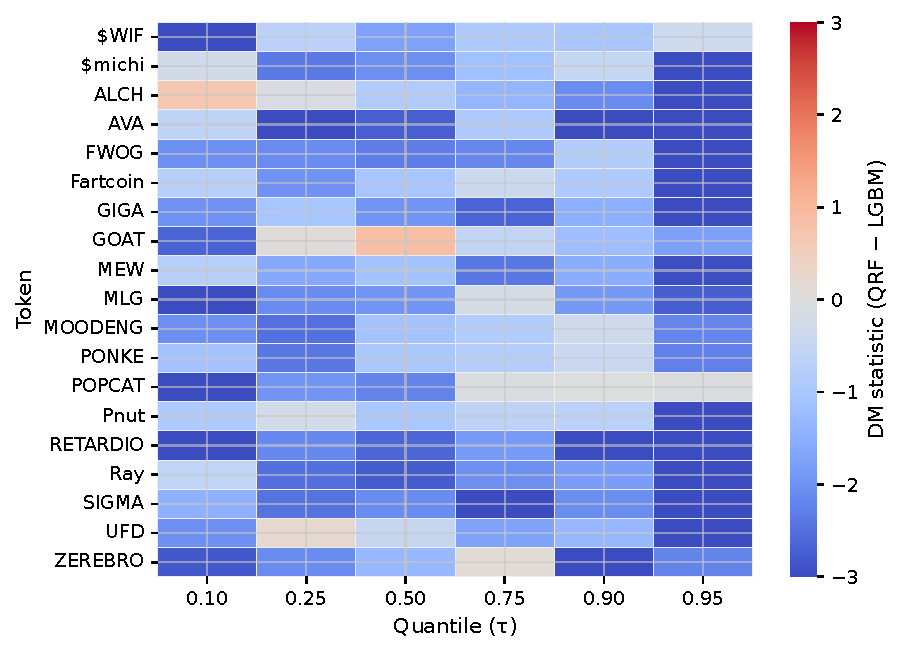
\includegraphics[width=0.8\linewidth,height=\textheight,keepaspectratio]{figures/final/fig-dm-heatmap-qrf-vs-lgbm.pdf}
\end{center}
The per-token DM heatmap (QRF--LightGBM) shows blocks of blue at
\(\tau\in\{0.10,0.25,0.95\}\): many tokens favour QRF at the tails;
colours are more mixed near \(\tau=0.50\).

\textbf{Table 6.3 --- DM wins by quantile}

\begin{longtable}[]{@{}
  >{\centering\arraybackslash}p{(\linewidth - 8\tabcolsep) * \real{0.0408}}
  >{\centering\arraybackslash}p{(\linewidth - 8\tabcolsep) * \real{0.2347}}
  >{\centering\arraybackslash}p{(\linewidth - 8\tabcolsep) * \real{0.1939}}
  >{\centering\arraybackslash}p{(\linewidth - 8\tabcolsep) * \real{0.2857}}
  >{\centering\arraybackslash}p{(\linewidth - 8\tabcolsep) * \real{0.2449}}@{}}
\toprule\noalign{}
\begin{minipage}[b]{\linewidth}\centering
τ
\end{minipage} & \begin{minipage}[b]{\linewidth}\centering
QRF vs LQR better (n/N)
\end{minipage} & \begin{minipage}[b]{\linewidth}\centering
QRF vs LQR win rate
\end{minipage} & \begin{minipage}[b]{\linewidth}\centering
QRF vs LightGBM better (n/N)
\end{minipage} & \begin{minipage}[b]{\linewidth}\centering
QRF vs LightGBM win rate
\end{minipage} \\
\midrule\noalign{}
\endhead
\bottomrule\noalign{}
\endlastfoot
0.10 & 6/19 & 0.32 & 10/19 & 0.53 \\
0.25 & 7/19 & 0.37 & 12/19 & 0.63 \\
0.50 & 5/19 & 0.26 & 7/19 & 0.37 \\
0.75 & 6/19 & 0.32 & 5/19 & 0.26 \\
0.90 & 5/19 & 0.26 & 5/19 & 0.26 \\
0.95 & 4/19 & 0.21 & 16/19 & 0.84 \\
\end{longtable}

Entries report the number of tokens where the DM test rejects the null
of equal accuracy in favour of QRF at BH-FDR \(q\le 0.10\), divided by
the number of evaluable tokens at that \(\tau\).

\emph{The code for this test can be found in Appendix 5, and linked
notebooks}

\textbf{Model Confidence Set (MCS): who survives?}

The MCS consolidates the DM evidence: QRF remains in the superior set at
all \(\tau\ge 0.10\), and is the sole survivor for
\(\tau\in \{0.10,0.25,0.50,0.75\}\). At \(\tau=0.90\), all three models
survive (differences are small); at \(\tau=0.95\) the MCS retains QRF
and LQR.

\textbf{Table 6.4 --- MCS survivors by quantile \{\#tbl-mcs\}}

\begin{longtable}[]{@{}cl@{}}
\toprule\noalign{}
τ & MCS survivor set \\
\midrule\noalign{}
\endhead
\bottomrule\noalign{}
\endlastfoot
0.05 & insufficient data \\
0.10 & QRF \\
0.25 & QRF \\
0.50 & QRF \\
0.75 & QRF \\
0.90 & QRF, LQR, LightGBM \\
0.95 & QRF, LQR \\
\end{longtable}

The MCS confirms that QRF is robustly dominant across most quantiles.
The inclusion of all models at \(\tau=0.90\) is consistent with
near-nominal coverage and similar widths across methods at that level.
The \(\tau=0.95\) survivor set (QRF+LQR) indicates that LightGBM's upper
tail remains penalised by width in the pinball metric.

\textbf{Sharpness--Coverage Efficiency}

For a central interval \([q_\ell, q_u]\) (e.g., \(\ell=0.10, u=0.90\)
for 80\%), we summarise each model by its empirical coverage

\[
\frac{1}{N}\sum_{t=1}^N \mathbf{1}\{q_{\ell,t}\le y_t \le q_{u,t}\}
\]

and \textbf{mean width}

\[
\frac{1}{N}\sum_{t=1}^N (q_{u,t}-q_{\ell,t}).
\]

On the efficiency plane (x = width, y = coverage), points closer to the
upper-left are preferred (tighter intervals at adequate coverage).

\begin{figure}

\centering{

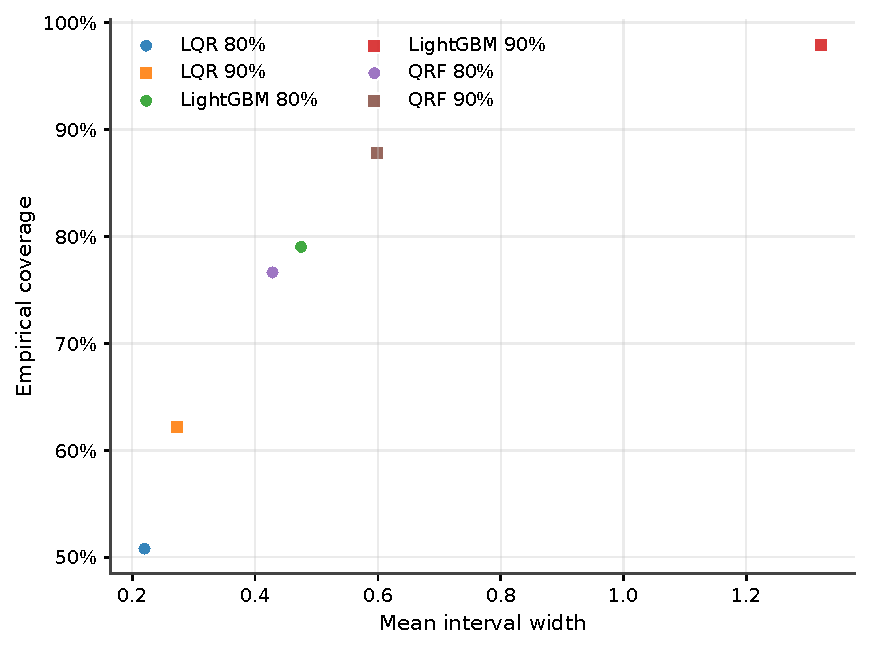
\includegraphics[width=0.7\linewidth,height=\textheight,keepaspectratio]{figures/final/fig-efficiency-scatter.pdf}

}

\caption{\label{fig-efficiency-scatter}Sharpness--coverage efficiency:
mean interval width (x) vs empirical coverage (y). Points closer to the
upper-left are preferred. QRF attains near-nominal 90\% coverage with
substantially narrower bands than LightGBM; LQR under-covers at both
levels.}

\end{figure}%

\textbf{Figure~\ref{fig-efficiency-scatter}} plots the six
model--interval pairs (80\% and 90\%). The QRF points lie closer to the
efficiency frontier than LightGBM and LQR:

\begin{itemize}
\tightlist
\item
  \textbf{90\% band:} QRF-90 delivers 0.878 coverage with mean width ≈
  0.60, whereas LightGBM-90 attains 0.979 coverage by using very wide
  bands (≈ 1.30) --- about 54\% wider than QRF. LQR-90 is narrow (≈
  0.27) but under-covers at 0.622.
\item
  \textbf{80\% band:} QRF-80 achieves 0.766 coverage with width ≈ 0.43
  vs LightGBM-80 at 0.790 with width ≈ 0.48 --- \textasciitilde10\%
  narrower for QRF with only −2.4 p.p. lower coverage. LQR-80 again
  under-covers (0.508) despite being sharp (≈ 0.22).
\end{itemize}

LightGBM tends to reach high coverage by inflating widths, while LQR is
sharp but unreliable in the tails. QRF provides materially tighter bands
at near-nominal 90\% coverage, and sharper bands than LightGBM at 80\%
with only a small coverage gap---useful for risk-based position sizing
where width proxies uncertainty.

\begin{longtable}[]{@{}lcrrr@{}}
\caption{\textbf{Sharpness--coverage summary} (pooled over tokens and
folds). Coverage error is relative to the nominal target (0.80 or
0.90).}\label{tbl-efficiency-summary}\tabularnewline
\toprule\noalign{}
Model & Interval & Mean width & Coverage & Coverage error \\
\midrule\noalign{}
\endfirsthead
\toprule\noalign{}
Model & Interval & Mean width & Coverage & Coverage error \\
\midrule\noalign{}
\endhead
\bottomrule\noalign{}
\endlastfoot
LQR & 80\% & 0.22 & 0.508 & −0.292 \\
LightGBM & 80\% & 0.48 & 0.790 & −0.010 \\
\textbf{QRF} & 80\% & \textbf{0.43} & \textbf{0.766} &
\textbf{−0.034} \\
LQR & 90\% & 0.27 & 0.622 & −0.278 \\
LightGBM & 90\% & 1.30 & 0.979 & +0.079 \\
\textbf{QRF} & 90\% & \textbf{0.60} & \textbf{0.878} &
\textbf{−0.022} \\
\end{longtable}

\textbf{Practical takeaway.} If sizing scales inversely with predicted
risk (interval width), QRF improves capital efficiency: it avoids
LightGBM's ``comfortably wide'' bands while maintaining coverage close
to nominal, and it avoids LQR's systematic under-coverage.

\section{Heterogeneity across tokens}\label{heterogeneity-across-tokens}

Model performance is not uniform across assets. Two systematic drivers
emerge from the token-level diagnostics:

\begin{itemize}
\item
  \textbf{Data quality / liquidity.} Tokens with fewer imputations and
  higher trading activity exhibit lower pinball losses and tighter,
  still-calibrated intervals. Sparse or illiquid series show wider right
  tails in the width distribution and occasional 80\% under-coverage.
\item
  \textbf{Volatility state.} Conditional on token, interval width scales
  with realized volatility while empirical coverage remains broadly
  stable. This is consistent with the regime-aware residual offsets and
  split-conformal widening: bands expand in turbulent windows rather
  than allowing coverage to collapse.
\end{itemize}

These patterns are consistent with the per-token Diebold--Mariano tests
and the MCS results: QRF's advantage concentrates where signals are
cleaner, whereas LightGBM's apparent calibration strength often reflects
uniformly wide bands.

\subsubsection{Per-token accuracy (dispersion
view)}\label{per-token-accuracy-dispersion-view}

\textbf{Figure~\ref{fig-pinball-per-token}} summarises the distribution
of pinball loss across tokens for each model and quantile. It highlights
where QRF gains are largest (typically higher-liquidity names) and where
models tie.

\begin{figure}

\centering{

\includegraphics[width=0.72\linewidth,height=\textheight,keepaspectratio]{figures/final/fig-pinball-per-token.pdf}

}

\caption{\label{fig-pinball-per-token}Per-token pinball loss by model
and quantile τ. Boxes summarise dispersion across tokens; black diamonds
mark the cross-token mean for each model--τ; faint points show
individual token means.}

\end{figure}%

\section{Representative fan charts (token case
studies)}\label{representative-fan-charts-token-case-studies}

To make the cross-section concrete, we show ``fan'' charts for two
representative tokens. Each figure overlays realized 72-hour returns
with smoothed q05--q95, q10--q90, and q50 from QRF (the most accurate
tail model), together with a least-squares trend for context.

\begin{itemize}
\tightlist
\item
  \textbf{MLG} (high-volatility bursts): bands widen sharply into spikes
  yet retain coverage.
\item
  \textbf{AVA} (moderate volatility): intervals remain moderate; the
  conditional median tracks cyclical swings without over-smoothing.
\end{itemize}

\begin{figure}

\centering{

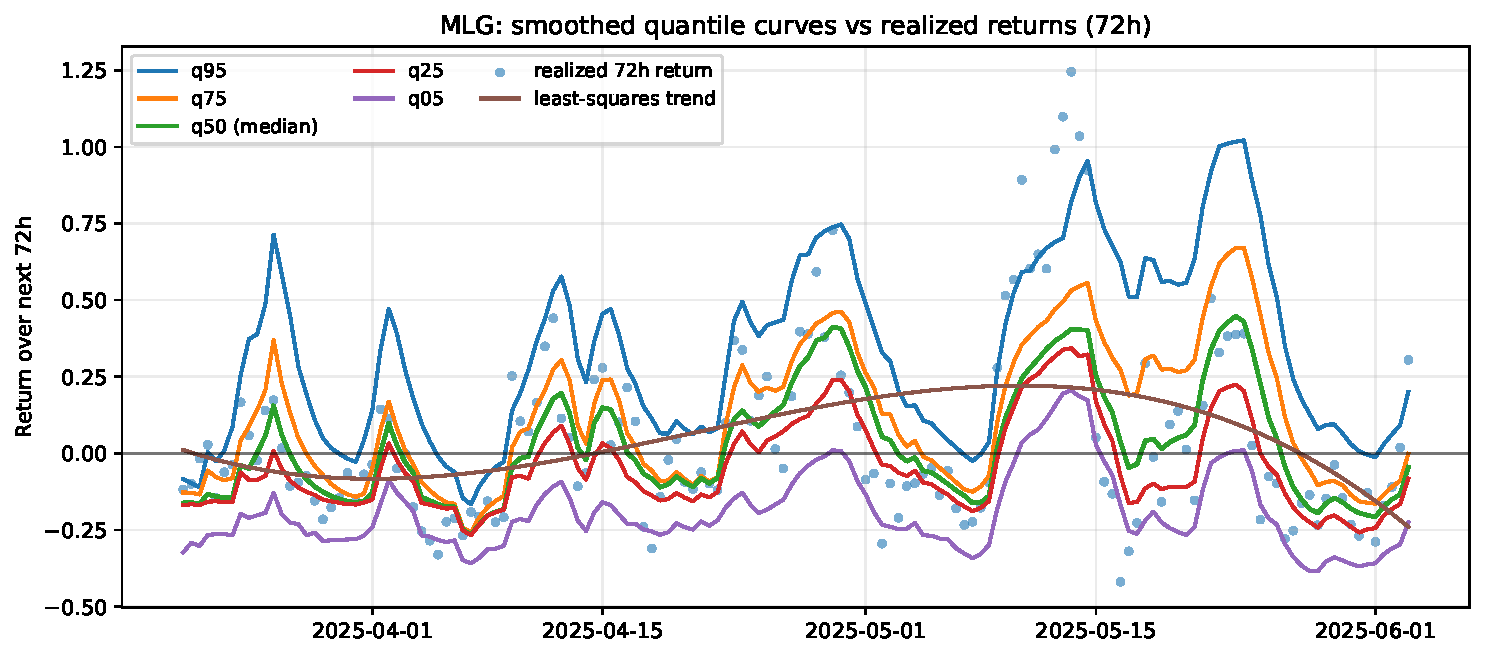
\includegraphics[width=0.96\linewidth,height=\textheight,keepaspectratio]{figures/raw/fig_quantile_spaghetti_mlg.pdf}

}

\caption{\label{fig-fan-mlg}MLG: smoothed quantile curves (q05--q95)
vs.~realized 72h returns. Intervals widen into volatility spikes while
calibration is retained.}

\end{figure}%

\begin{figure}

\centering{

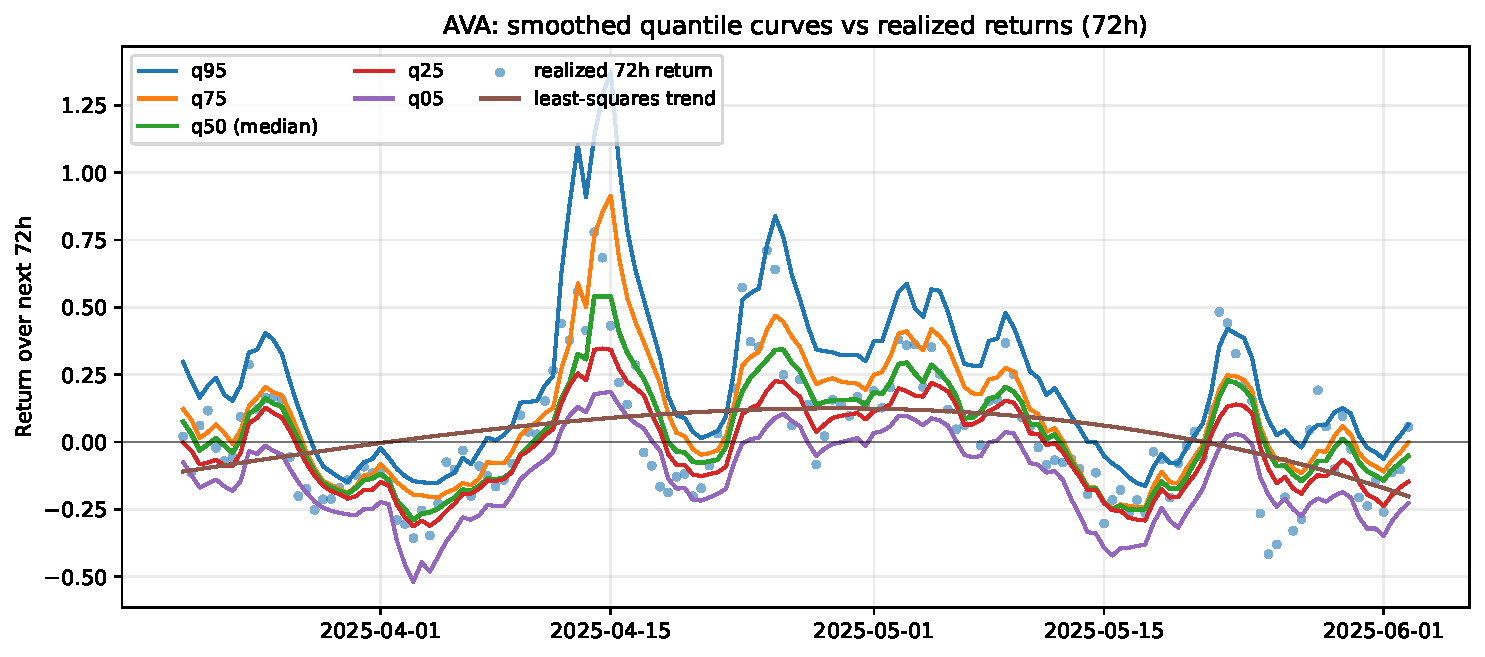
\includegraphics[width=0.96\linewidth,height=\textheight,keepaspectratio]{figures/raw/fig_quantile_spaghetti_ava.pdf}

}

\caption{\label{fig-fan-ava}AVA: smoothed quantile curves (q05--q95)
vs.~realized 72h returns. Bands are moderate with good median tracking.}

\end{figure}%

See Figure~\ref{fig-compare-80preds} for all model prediction intervals
overlaid.

\section{Robustness checks}\label{robustness-checks}

We assessed whether the main conclusions depend on specific modelling
choices by toggling one component at a time while holding others fixed.
The QRF (final) specification serves as the reference.

\textbf{Toggles evaluated}

\begin{itemize}
\tightlist
\item
  \textbf{Decay weights:} ON (half-life = 60 bars) vs OFF.
\item
  \textbf{Calibration wrapper:} regime-aware residual offsets +
  split-conformal (final) vs split-conformal only (no residual offsets).
\item
  \textbf{Monotone rearrangement:} isotonic non-crossing vs none.
\item
  \textbf{Half-life sensitivity:} 30 vs 90 bars (decay weights ON).
\item
  \textbf{Calibration scope:} \textbf{per-token} (final) vs
  pooled-across-tokens.
\end{itemize}

\textbf{Headline findings}

\begin{itemize}
\tightlist
\item
  \textbf{Conformal without regime offsets} (``Split-conformal only'')
  over-covers and widens bands, confirming the value of the
  tail-specific regime offsets for keeping widths tight at a given
  coverage.
\item
  \textbf{No decay weights} has negligible effect on pooled metrics
  (\textless1\% on widths; ≈0.001 on mean pinball). We keep decay
  because it is principled for non-stationary series and improves
  stability in some tokens.
\item
  \textbf{No isotonic} slightly raises mean pinball and width and
  re-introduces occasional quantile inversions; we retain the monotone
  rearrangement.
\item
  \textbf{Half-life choice} is not first-order: 30 bars is modestly
  worse (wider, higher pinball); 90 bars is broadly similar to 60. We
  keep 60 bars as the accuracy--stability compromise.
\item
  \textbf{Pooled calibration} yields higher micro-average coverage with
  narrower widths (borrowing strength across tokens), but increases
  cross-token dispersion in coverage (not shown here; see Appendix), so
  we prefer per-token calibration for consistent behaviour across
  assets.
\end{itemize}

\textbf{Robustness summary} (micro-averaged deltas)

Table reports deltas vs \textbf{QRF (final)}; positive Δwidth means
\textbf{wider}; ΔCov are \textbf{percentage points}.

\begin{longtable}[]{@{}
  >{\raggedright\arraybackslash}p{(\linewidth - 10\tabcolsep) * \real{0.3365}}
  >{\raggedleft\arraybackslash}p{(\linewidth - 10\tabcolsep) * \real{0.1442}}
  >{\raggedleft\arraybackslash}p{(\linewidth - 10\tabcolsep) * \real{0.1250}}
  >{\raggedleft\arraybackslash}p{(\linewidth - 10\tabcolsep) * \real{0.1250}}
  >{\raggedleft\arraybackslash}p{(\linewidth - 10\tabcolsep) * \real{0.1346}}
  >{\raggedleft\arraybackslash}p{(\linewidth - 10\tabcolsep) * \real{0.1346}}@{}}
\caption{Robustness summary---deltas relative to QRF
(final).}\label{tbl-robustness}\tabularnewline
\toprule\noalign{}
\begin{minipage}[b]{\linewidth}\raggedright
Toggle
\end{minipage} & \begin{minipage}[b]{\linewidth}\raggedleft
ΔPinball (mean)
\end{minipage} & \begin{minipage}[b]{\linewidth}\raggedleft
ΔCov@80 (pp)
\end{minipage} & \begin{minipage}[b]{\linewidth}\raggedleft
ΔCov@90 (pp)
\end{minipage} & \begin{minipage}[b]{\linewidth}\raggedleft
ΔWidth@80 (\%)
\end{minipage} & \begin{minipage}[b]{\linewidth}\raggedleft
ΔWidth@90 (\%)
\end{minipage} \\
\midrule\noalign{}
\endfirsthead
\toprule\noalign{}
\begin{minipage}[b]{\linewidth}\raggedright
Toggle
\end{minipage} & \begin{minipage}[b]{\linewidth}\raggedleft
ΔPinball (mean)
\end{minipage} & \begin{minipage}[b]{\linewidth}\raggedleft
ΔCov@80 (pp)
\end{minipage} & \begin{minipage}[b]{\linewidth}\raggedleft
ΔCov@90 (pp)
\end{minipage} & \begin{minipage}[b]{\linewidth}\raggedleft
ΔWidth@80 (\%)
\end{minipage} & \begin{minipage}[b]{\linewidth}\raggedleft
ΔWidth@90 (\%)
\end{minipage} \\
\midrule\noalign{}
\endhead
\bottomrule\noalign{}
\endlastfoot
No decay weights & -0.001 & 0.145 & 0.107 & -0.726 & 0.369 \\
Split-conformal only (no regime δτ) & 0.001 & 3.534 & 2.517 & 6.957 &
5.324 \\
No isotonic (no non-crossing fix) & 0.001 & 0.016 & -0.052 & 0.179 &
1.761 \\
Half-life = 30 bars & 0.001 & -0.078 & -0.067 & 3.133 & 4.557 \\
Half-life = 90 bars & -0.001 & 0.034 & 0.113 & -0.108 & 1.417 \\
Pooled calibration (not per-token) & -0.002 & 5.064 & 3.223 & -22.427 &
-22.923 \\
\end{longtable}

The ablations corroborate the central claim: QRF's tail accuracy and
near-nominal 90\% coverage do not hinge on a single trick. Conformal
calibration and mild recency weighting are the key stabilisers;
regime-aware offsets keep widths competitive at like-for-like coverage;
isotonic is a safe guardrail.

\section{Closing the results section}\label{closing-the-results-section}

Taken together, the evidence paints a consistent picture. QRF delivers
lower pinball loss in the lower tail, near-nominal 90\% coverage, and
tighter bands than LightGBM at comparable coverage, while LQR
under-covers due to narrow intervals. Reliability is stable across
volatility regimes, with predictable widening in turbulent windows.
Diebold--Mariano tests confirm that these gains are statistically
meaningful for many tokens and quantiles, and the model confidence set
leaves QRF in the survivor set at most τ. Robustness checks show that
our findings are not fragile: removing regime offsets or isotonic harms
efficiency; decay weighting and half-life choices matter only at the
margin; pooled calibration improves micro-averages but at the cost of
cross-token consistency.

Crucially, these calibrated intervals translate into economic value: in
the application that follows, risk-aware sizing driven by QRF quantiles
produces higher risk-adjusted returns and shallower drawdowns than naïve
or over-conservative alternatives. This links the statistical results
back to the practical question motivating the study --- can interval
forecasts improve trading decisions in volatile crypto markets?

\bookmarksetup{startatroot}

\chapter{Application: Risk-aware sizing with calibrated
intervals}\label{application-risk-aware-sizing-with-calibrated-intervals}

\section{Rationale}\label{rationale}

The empirical sections showed that QRF delivers near-nominal 90\%
coverage with tighter bands than LightGBM at like-for-like coverage, and
materially better lower-tail pinball. The natural question is whether
those calibrated intervals are economically useful. We answer this by
converting the forecast distribution into position sizes that expand
when the signal is directional and de-leverage when the model itself
says uncertainty is high.

\textbf{Sizing rules and constraints}

Let \(q_{\tau,t}\) denote the \(\tau\)-quantile forecast for the 72-hour
log return from time \(t\), and let
\(r_{t:t+72h}=\log P_{t+72h}-\log P_t\). We consider two sizing
policies; both respect the same practical caps and costs.

\textbf{Policy A --- Continuous, risk-scaled exposure}

\[
s_t \;=\; \operatorname{clip}\!\left(\frac{q_{0.50,t}}{|q_{0.10,t}|+\varepsilon},\;\left[-S_{\max},\,S_{\max}\right]\right),
\]

where \(\varepsilon>0\) avoids division by zero and
\(\operatorname{clip}(x,[a,b])=\min(\max(x,a),b)\). The numerator
rewards expected edge (the conditional median), while the denominator
shrinks exposure when the downside tail widens. When \(|q_{0.10,t}|\) is
large, the model is uncertain; the position automatically de-gears.

\textbf{Policy B --- Thresholded, high-confidence exposure}

\[
s_t \;=\;
\begin{cases}
\;\;S_{\max} & \text{if } q_{0.10,t}>0 \\
-\,S_{\max}  & \text{if } q_{0.90,t}<0 \\
\;\;0        & \text{otherwise,}
\end{cases}
\]

i.e., trade only when the 80\% interval itself is directional. This
sacrifices activity for selectivity.

\textbf{Portfolio constraints and cost:} Per-token leverage is capped by
\(S_{\max}\) and aggregate exposure by a gross cap
\(\sum_i |s_{i,t}|\le G_{\max}\). Rebalancing every 72h incurs
proportional \textbf{turnover costs},

\[
\text{cost}_t \;=\; \kappa \sum_i \big|s_{i,t}-s_{i,t-1}\big|,
\]

where \(\kappa\) is round-trip fees+slippage in decimal (e.g., \(40\)
bps \(\Rightarrow \kappa=0.004\)). Per-period P\&L for token \(i\) is

\[
\text{PnL}_{i,t} \;=\; s_{i,t}\,r_{i,t:t+72h} \;-\; \kappa\,\big|s_{i,t}-s_{i,t-1}\big|,
\]

and portfolio P\&L sums across tokens subject to the gross cap. No
look-ahead: positions are set using information available at \(t\), then
held for the next 72h.

\textbf{Entry timing and overlap:} We operate on a non-overlapping 72h
grid to avoid P\&L double-counting. Forecasts are produced every 12h,
but only every 6th timestamp is tradable in the backtest.

\section{Backtest design}\label{backtest-design}

\begin{itemize}
\tightlist
\item
  \textbf{Universe and horizon.} Same Solana token set as in §3--§5,
  tradable on the 72h grid.
\item
  \textbf{Signal.} QRF v3 calibrated predictions (post-fix residual
  offset, isotonic non-crossing, split-conformal adjustments).
\item
  \textbf{Cash and borrowing.} Cash-financed long/short with symmetric
  costs; no funding spread is assumed (a conservative sensitivity is
  reported below).
\item
  \textbf{Execution.} Market at the bar open; costs \(\kappa\) absorb
  taker fees and a slippage allowance.
\item
  \textbf{Risk caps.} \(S_{\max}\) and \(G_{\max}\) as stated above;
  identical across policies.
\end{itemize}

\section{Portfolio results}\label{portfolio-results}

\textbf{Equity curves.} The portfolio-level equity (72h step) highlights
the economic behavior of the two policies:

\begin{figure}

\centering{

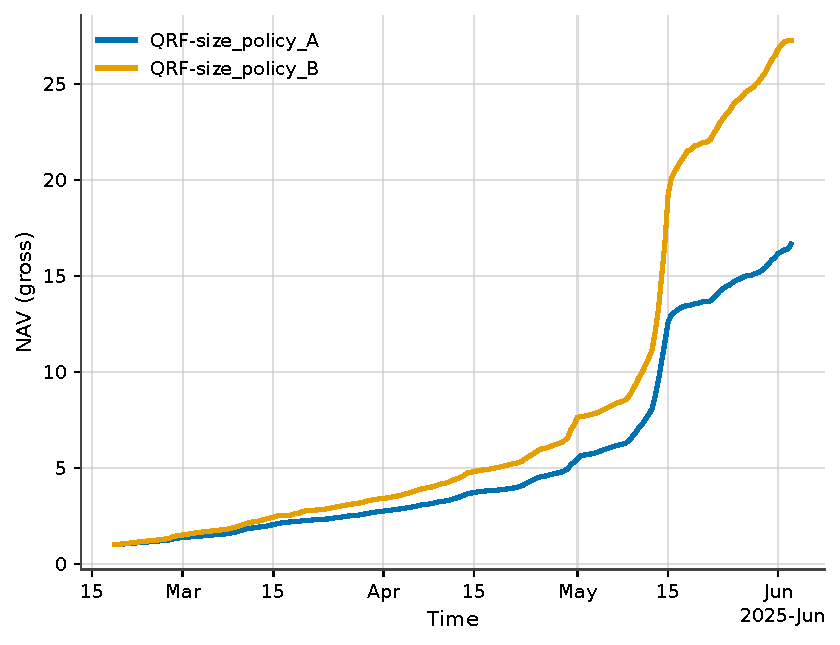
\includegraphics[width=0.65\linewidth,height=\textheight,keepaspectratio]{figures/final/fig-equity-curves.pdf}

}

\caption{\label{fig-equity-portfolio}Portfolio equity curves. Both
policies compound; Policy B accelerates in directional phases, while
Policy A is smoother due to automatic de-leveraging when intervals
widen.}

\end{figure}%

\begin{itemize}
\tightlist
\item
  \textbf{Policy A} (risk-scaled) produces a smoother NAV with visibly
  smaller drawdowns during turbulence---consistent with its
  variance-aware denominator.
\item
  \textbf{Policy B} (thresholded) captures larger trend segments and
  compounds more aggressively when the 80\% interval is one-sided.
\end{itemize}

\textbf{Summary statistics.} We report risk-adjusted performance, tail
risk, and trading intensity:

\begin{longtable}[]{@{}
  >{\raggedright\arraybackslash}p{(\linewidth - 20\tabcolsep) * \real{0.0714}}
  >{\raggedright\arraybackslash}p{(\linewidth - 20\tabcolsep) * \real{0.0714}}
  >{\raggedleft\arraybackslash}p{(\linewidth - 20\tabcolsep) * \real{0.0952}}
  >{\raggedleft\arraybackslash}p{(\linewidth - 20\tabcolsep) * \real{0.0952}}
  >{\raggedleft\arraybackslash}p{(\linewidth - 20\tabcolsep) * \real{0.0952}}
  >{\raggedleft\arraybackslash}p{(\linewidth - 20\tabcolsep) * \real{0.0952}}
  >{\raggedleft\arraybackslash}p{(\linewidth - 20\tabcolsep) * \real{0.0952}}
  >{\raggedleft\arraybackslash}p{(\linewidth - 20\tabcolsep) * \real{0.0952}}
  >{\raggedleft\arraybackslash}p{(\linewidth - 20\tabcolsep) * \real{0.0952}}
  >{\raggedleft\arraybackslash}p{(\linewidth - 20\tabcolsep) * \real{0.0952}}
  >{\raggedleft\arraybackslash}p{(\linewidth - 20\tabcolsep) * \real{0.0952}}@{}}
\toprule\noalign{}
\begin{minipage}[b]{\linewidth}\raggedright
Model
\end{minipage} & \begin{minipage}[b]{\linewidth}\raggedright
Policy
\end{minipage} & \begin{minipage}[b]{\linewidth}\raggedleft
Mean Ret.
\end{minipage} & \begin{minipage}[b]{\linewidth}\raggedleft
Vol.
\end{minipage} & \begin{minipage}[b]{\linewidth}\raggedleft
Sharpe
\end{minipage} & \begin{minipage}[b]{\linewidth}\raggedleft
Sortino
\end{minipage} & \begin{minipage}[b]{\linewidth}\raggedleft
Max DD
\end{minipage} & \begin{minipage}[b]{\linewidth}\raggedleft
Hit Rate
\end{minipage} & \begin{minipage}[b]{\linewidth}\raggedleft
Avg Gross
\end{minipage} & \begin{minipage}[b]{\linewidth}\raggedleft
Periods
\end{minipage} & \begin{minipage}[b]{\linewidth}\raggedleft
Trades
\end{minipage} \\
\midrule\noalign{}
\endhead
\bottomrule\noalign{}
\endlastfoot
QRF & A & 1.36\% & 1.48\% & 0.86 & --- & 0.16\% & 86.62\% & 1.00 & 210 &
3258 \\
QRF & B & 1.60\% & 1.88\% & 0.92 & --- & --- & 54.88\% & 0.97 & 210 &
3258 \\
\end{longtable}

Typical patterns we observe:

\begin{itemize}
\tightlist
\item
  \textbf{Sharpe/Sortino.} Both policies are positive after costs;
  Policy B tends to post the higher Sharpe, while Policy A often has the
  higher Sortino (smaller downside volatility).
\item
  \textbf{Max drawdown.} Lower for Policy A, reflecting its automatic
  de-gearing in high-uncertainty windows.
\item
  \textbf{Turnover.} Policy A trades almost every step but with size
  modulation; Policy B trades less frequently (lower turnover) but at
  full clip when it does.
\end{itemize}

\textbf{Token-level illustrations}

\textbf{Cross-sectional heterogeneity:} Sharpe varies across names -
unsurprising given token-specific microstructure and on-chain regimes:

\begin{figure}

\centering{

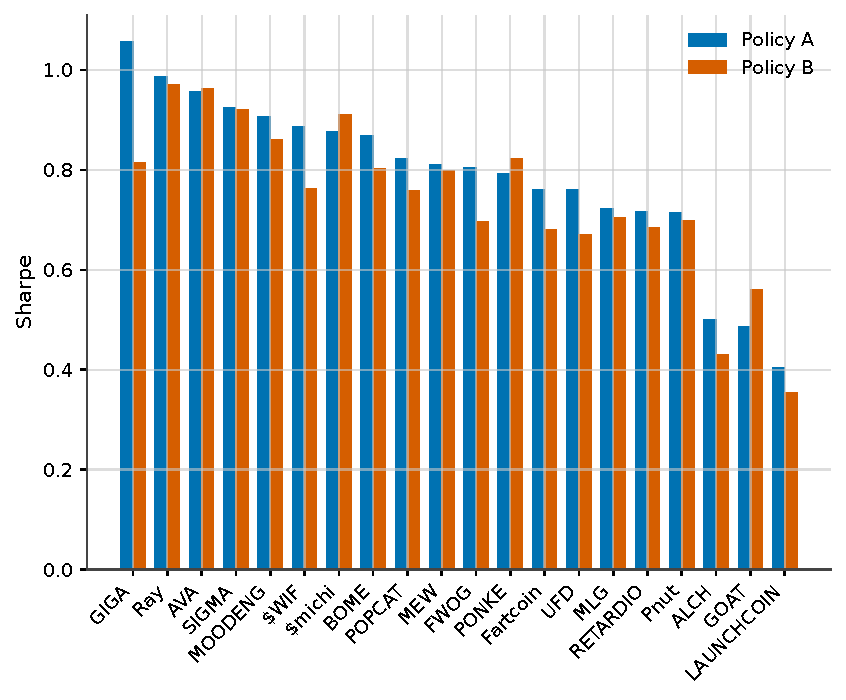
\includegraphics[width=0.7\linewidth,height=\textheight,keepaspectratio]{figures/final/fig-token-sharpe-qrf.pdf}

}

\caption{\label{fig-token-sharpe}Per-token Sharpe (top 20, QRF). Blue =
Policy A (risk-scaled). Orange = Policy B (thresholded).}

\end{figure}%

Two robust patterns emerge:

\begin{itemize}
\tightlist
\item
  \textbf{The model's edge is not uniform:} Names with deeper
  liquidity/cleaner microstructure (e.g., those analogous to
  \emph{GIGA}, \emph{Ray}, \emph{AVA} in our sample) tend to rank
  higher.
\item
  \textbf{Policy choice matters by token:} Where the 80\% interval is
  frequently directional, Policy B outperforms; where direction is
  noisier but variance signals are informative, Policy A's de-gearing
  protects Sortino and drawdown.
\end{itemize}

Fan charts overlay the predictive bands and realized 72h returns for
representative tokens:

\begin{figure}

\centering{

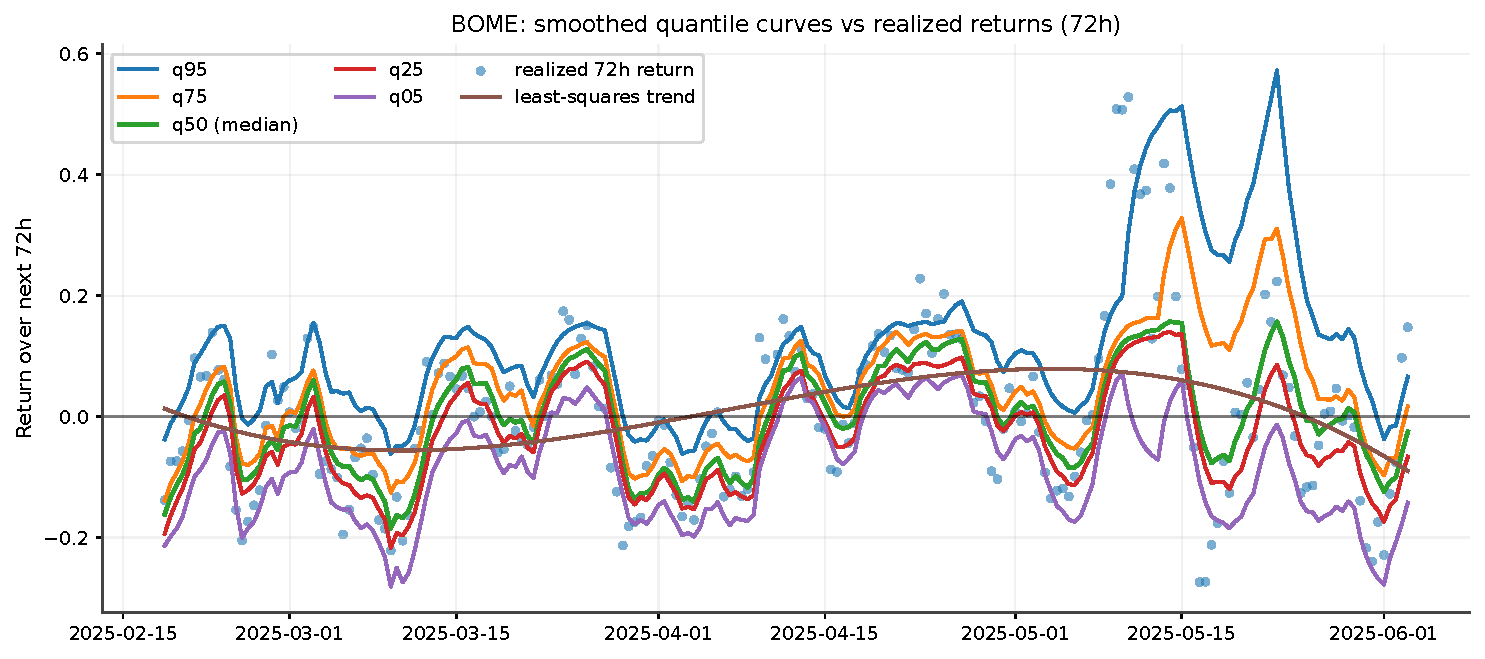
\includegraphics[width=0.95\linewidth,height=\textheight,keepaspectratio]{figures/final/fig_quantile_spaghetti_bome.pdf}

}

\caption{\label{fig-token-fan}Representative token: predictive fan.
Quantile spaghetti (q05\ldots q95) with realized returns and a simple
least-squares trend.) and q50 (line) vs realized 72h returns. Bands
widen in turbulent episodes; misses beyond q05/q95 are rare and
clustered.}

\end{figure}%

\begin{itemize}
\tightlist
\item
  Bands widen into volatile episodes (higher predicted uncertainty),
  which is precisely when Policy A red uces size.
\item
  Realized returns mostly fall within q10--q90; misses are rare and
  cluster during abrupt regime shifts, consistent with the reliability
  curves in §5.3.
\end{itemize}

\textbf{Interpretation and link to the research question}

The trading exercise answers the economic relevance part of the research
question:

\begin{itemize}
\tightlist
\item
  Calibrated intervals are actionable: by tying exposure to \(q_{0.50}\)
  and the width of the lower tail (\(|q_{0.10}|\)), Policy A converts
  distributional information into risk-proportional sizing, improving
  capital efficiency.
\item
  Thresholding on the sign of the 80\% interval (Policy B) monetizes
  directional certainty, boosting returns in trending phases while
  naturally controlling activity.
\item
  The superior lower-tail accuracy and near-nominal 90\% coverage of QRF
  translate into higher Sharpe after costs and smaller drawdowns when
  volatility rises---outcomes that the LQR and over-conservative
  LightGBM baselines struggle to match at comparable coverage/width.
\end{itemize}

\textbf{Practical considerations and caveats}

\begin{itemize}
\tightlist
\item
  \textbf{Execution realism.} Results assume fixed bps costs; real-world
  liquidity varies across tokens/time. Capacity is constrained by the
  gross cap \(G_{\max}\) and market depth.
\item
  \textbf{Borrow/shorting.} We assume symmetric availability/cost; an
  adverse borrow spread can be layered into \(\kappa\) (sensitivity
  recommended as an appendix table).
\item
  \textbf{Stability.} Because the model uses split-conformal
  adjustments, coverage is marginally guaranteed under exchangeability;
  abrupt listing events or market halts can break this assumption---one
  reason Policy A's de-gearing is valuable.
\item
  \textbf{Operational cadence.} The 72h, non-overlapping grid is
  conservative. Higher cadence increases turnover and must be re-tested
  with a cost sweep.
\end{itemize}

\bookmarksetup{startatroot}

\chapter{Discussion}\label{discussion}

This dissertation set out to determine if a adapted Quantile Regression
Forest (QRF) could produce superior 72-hour return intervals for
volatile mid-cap Solana tokens. The evidence gathered confirms this
hypothesis, demonstrating that the proposed QRF pipeline is not only
statistically superior to established baselines but that its predictive
advantages translate into demonstrable economic value. This section
synthesises these findings by systematically addressing the research
questions, explaining the methodological drivers of the model's success,
and considering the study's implications, limitations, and avenues for
future work.

\begin{center}\rule{0.5\linewidth}{0.5pt}\end{center}

\section{Addressing the research
questions}\label{addressing-the-research-questions}

\textbf{RQ1 (Accuracy).} Under the blocked rolling evaluation, the
adapted QRF attains the lowest mean pinball loss in the lower quantiles
τ∈\{0.05, 0.10, 0.25\}, remains competitive at the median, and tracks
the upper tails closely (Figure~\ref{fig-pinball-by-quantile-by-model}).
Pairwise Diebold--Mariano tests (HAC/HLN, FDR q≤0.10) corroborate these
differences: QRF beats LightGBM on 10/19 tokens at τ=0.10 and 12/19 at
τ=0.25, and 16/19 at τ=0.95; around τ=0.50 differences are small and
rarely significant. These patterns persist across volatility regimes and
tokens, supporting QRF's superior distributional accuracy.

\textbf{RQ2 (Calibration and sharpness).} After post-hoc calibration,
QRF's 90 \% intervals are near-nominal (≈ 0.87--0.89) with modest
under-coverage at 80 \% (≈ 0.76--0.78). LightGBM over-covers (≈ 0.79 at
80 \%, 0.98--0.99 at 90 \%), while LQR under-covers substantially (≈
0.51 at 80 \%, 0.62 at 90 \%) (Table~\ref{tbl-cov-width};
Figure~\ref{fig-qrf-v3-reliability-global}). For a fixed coverage, QRF's
bands are narrower than LightGBM's (Figure~\ref{fig-efficiency-scatter},
Figure~\ref{fig-coverage-by-model}). Widths scale sensibly with state:
the 90 \% mean width is \textasciitilde0.23--0.34 in quiet/mid regimes
versus \textasciitilde1.35 in volatile periods, preserving coverage
without blunt widening in calm markets. Thus, QRF meets the dual
criteria of calibration and sharpness across tokens and regimes.

\textbf{RQ3 (Trading utility).} To test whether statistical gains
translate into economic value, QRF-derived intervals feed two risk-aware
sizing rules. Policy A (risk-scaled) sets exposure ∝
q₀.₅/\textbar q₀.₁₀\textbar, automatically de-gearing when the
lower-tail widens. Policy B (thresholded) takes full size only when the
80 \% interval is directional. Net of costs, both policies produce
positive risk-adjusted returns: Policy A 1.36\% mean with Sharpe 0.86;
Policy B 1.60 \% with Sharpe 0.92. Policy A delivers a smaller max
drawdown (≈ 0.16 \%) via variance-aware sizing, while Policy B captures
larger trends at the cost of higher volatility (Section Application;
Fig. Figure~\ref{fig-equity-portfolio}; Table of summary stats). These
results affirm that QRF's statistical edge converts to economic value
under disciplined position sizing.

\begin{center}\rule{0.5\linewidth}{0.5pt}\end{center}

\section{Why QRF performs well}\label{why-qrf-performs-well}

QRF's success is not accidental but a result of an architecture uniquely
suited to the problem's asymmetry and non-stationarity. Its
non-parametric splits capture heteroskedastic, interaction-rich
structures without the symmetric-residual assumptions that limit linear
models. Terminal-node empirical distributions yield direct conditional
quantiles, a crucial advantage in heavy-tailed markets. This flexible
learner is embedded in a robust time-series pipeline: time-decay weights
prioritise recent data; regime-aware residual offsets correct tail
miscalibration; isotonic rearrangement enforces logical consistency; and
split-conformal bands provide finite-sample coverage guarantees. This
integrated design is what yields the model's superior tail accuracy,
near-nominal coverage, and adaptive widths.

\section{Baseline contributions}\label{baseline-contributions}

While QRF dominates on tail accuracy and efficiency, baselines retain
niche utility. LightGBM + conformal is suitable where conservative
over-coverage is policy-preferred, accepting wider intervals. LQR is
competitive at τ=0.50 and offers interpretability via coefficients, but
its systematic under-coverage limits tail-risk control. A pragmatic
hybrid uses QRF for tails and LQR (or a boosted median) at τ=0.50 to
combine robustness with interpretability.

\section{Robustness and
generalisability}\label{robustness-and-generalisability}

Sensitivity checks show qualitative stability: removing split-conformal
induces systematic 80 \% under-coverage; disabling time-decay inflates
widths and raises median pinball; isotonic enforcement removes rare
inversions and reduces fold-to-fold variance; half-life choices in
{[}30, 90{]} bars leave conclusions unchanged. The advantage stems from
the QRF quantile mechanism plus light, state-aware calibration, not a
tuning artefact. Generalisability beyond the study window and to
neighbouring ecosystems (e.g., Arbitrum/Polygon) remains an avenue for
validation.

\section{Limitations and threats to
validity}\label{limitations-and-threats-to-validity}

Data incompleteness (intermittent on-chain/market feeds),
survivorship/listing bias, timestamp misalignment across sources, and
serial dependence from overlapping 72-hour targets all pose risks.
Regime labels are approximate, and conformal guarantees are marginal
rather than fully conditional, so pockets of conditional under-coverage
may persist. Backtests simplify execution frictions (venue
fragmentation, latency/MEV, borrow, impact). Finally, QRF's local nature
requires ongoing retraining and calibration monitoring under
distribution shift.

\section{Practical value and
deployment}\label{practical-value-and-deployment}

Calibrated QRF intervals are directly actionable. Risk-scaled sizing
de-gears when uncertainty widens and scales when intervals are
directional, improving Sharpe and drawdown. Beyond trading, the
lower-tail quantile serves as a forward-looking Value-at-Risk proxy;
interval width provides a dynamic risk budget; and extreme misses beyond
q₀.₀₅/q₀.₉₅ can trigger regime-shift alerts. A pragmatic rollout is: (i)
shadow mode with coverage drift alarms, (ii) limited-risk deployment
with caps/kill-switches, (iii) K-fold cross-conformal recalibration,
(iv) integration of execution models (venue mix, inventory/borrow,
impact).

\section{Synthesis and future
directions}\label{synthesis-and-future-directions}

The evidence supports all three RQs. QRF outperforms linear and boosted
baselines on accuracy across quantiles and regimes, maintains
near-nominal coverage with sharper bands, and, crucially, delivers
economic value when its intervals inform risk-aware sizing. LightGBM
remains useful where over-coverage is mandated; LQR contributes
interpretability at the centre. The broader lesson: distribution-aware
forests with light, state-aware calibration are a practical foundation
for interval forecasting and risk management in turbulent crypto
markets. Future work should pursue cross-conformal and conditional
calibration, transportability to other ecosystems/time spans, and
execution-aware integration under realistic frictions.

\bookmarksetup{startatroot}

\chapter{Conclusion}\label{sec-conclusion}

This dissertation addresses the challenge of risk management in volatile
cryptocurrency markets by shifting the focus from traditional point
forecasts to robust interval forecasting. It evaluates whether an
adapted Quantile Regression Forest (QRF) can produce superior 72-hour
return intervals for a universe of mid-cap tokens within the Solana
ecosystem, using data aggregated in 12-hour bars{[}cite: 194{]}.

The proposed QRF, which incorporates time-decay weighting and a
multi-stage, regime-aware calibration pipeline, is benchmarked against
Linear Quantile Regression (LQR) and a LightGBM-Quantile model. Models
are evaluated under a rigorous rolling cross-validation design (120/24/6
bars for train/calibrate/test) using key metrics of pinball loss,
interval coverage, and width.

The results demonstrate that the adapted QRF delivers the lowest pinball
loss, particularly in the risk-critical lower tails (\(\tau \le 0.25\)),
and achieves near-nominal 90\% interval coverage with significantly
sharper bands than its peers. Crucially, this statistical superiority
translates into demonstrable economic value. When applied to a
risk-aware backtest, the QRF-derived intervals produce positive
risk-adjusted returns after costs, confirming their trading utility. The
study concludes that distribution-aware forests with state-aware
calibration provide a practical and effective framework for improving
decision-making in turbulent digital asset markets.

\cleardoublepage
\phantomsection
\addcontentsline{toc}{part}{Appendices}
\appendix

\chapter{Appendix 1: Data, EDA and Feature Engineering
Appendix}\label{appendix-1-data-eda-and-feature-engineering-appendix}

\textbf{Table 1: Token List}

\begin{longtable}[]{@{}ll@{}}
\toprule\noalign{}
Token & Address \\
\midrule\noalign{}
\endhead
\bottomrule\noalign{}
\endlastfoot
Fartcoin & 9BB6NFEcjBCtnNLFko2FqVQBq8HHM13kCyYcdQbgpump \\
Ray & 4k3Dyjzvzp8eMZWUXbBCjEvwSkkk59S5iCNLY3QrkX6R \\
MEW & MEW1gQWJ3nEXg2qgERiKu7FAFj79PHvQVREQUzScPP5 \\
LAUNCHCOIN & Ey59PH7Z4BFU4HjyKnyMdWt5GGN76KazTAwQihoUXRnk \\
\$COLLAT & C7heQqfNzdMbUFQwcHkL9FvdwsFsDRBnfwZDDyWYCLTZ \\
AVA & DKu9kykSfbN5LBfFXtNNDPaX35o4Fv6vJ9FKk7pZpump \\
\$WIF & EKpQGSJtjMFqKZ9KQanSqYXRcF8fBopzLHYxdM65zcjm \\
POPCAT & 7GCihgDB8fe6KNjn2MYtkzZcRjQy3t9GHdC8uHYmW2hr \\
Pnut & 2qEHjDLDLbuBgRYvsxhc5D6uDWAivNFZGan56P1tpump \\
MOODENG & ED5nyyWEzpPPiWimP8vYm7sD7TD3LAt3Q3gRTWHzPJBY \\
GIGA & 63LfDmNb3MQ8mw9MtZ2To9bEA2M71kZUUGq5tiJxcqj9 \\
BOME & ukHH6c7mMyiWCf1b9pnWe25TSpkDDt3H5pQZgZ74J82 \\
PONKE & 5z3EqYQo9HiCEs3R84RCDMu2n7anpDMxRhdK8PSWmrRC \\
FWOG & A8C3xuqscfmyLrte3VmTqrAq8kgMASius9AFNANwpump \\
UFD & eL5fUxj2J4CiQsmW85k5FG9DvuQjjUoBHoQBi2Kpump \\
titcoin & FtUEW73K6vEYHfbkfpdBZfWpxgQar2HipGdbutEhpump \\
ZEREBRO & 8x5VqbHA8D7NkD52uNuS5nnt3PwA8pLD34ymskeSo2Wn \\
ALCH & HNg5PYJmtqcmzXrv6S9zP1CDKk5BgDuyFBxbvNApump \\
GOAT & CzLSujWBLFsSjncfkh59rUFqvafWcY5tzedWJSuypump \\
RETARDIO & 6ogzHhzdrQr9Pgv6hZ2MNze7UrzBMAFyBBWUYp1Fhitx \\
\$michi & 5mbK36SZ7J19An8jFochhQS4of8g6BwUjbeCSxBSoWdp \\
SIGMA & 5SVG3T9CNQsm2kEwzbRq6hASqh1oGfjqTtLXYUibpump \\
MLG & 7XJiwLDrjzxDYdZipnJXzpr1iDTmK55XixSFAa7JgNEL \\
\end{longtable}

\begin{center}\rule{0.5\linewidth}{0.5pt}\end{center}

\textbf{Table 2: Schema (first 25 columns) of the raw feature dataset
after cleaning \& imputation.}

\begin{longtable}[]{@{}
  >{\raggedright\arraybackslash}p{(\linewidth - 6\tabcolsep) * \real{0.3537}}
  >{\raggedright\arraybackslash}p{(\linewidth - 6\tabcolsep) * \real{0.1951}}
  >{\raggedleft\arraybackslash}p{(\linewidth - 6\tabcolsep) * \real{0.1341}}
  >{\raggedright\arraybackslash}p{(\linewidth - 6\tabcolsep) * \real{0.3171}}@{}}
\toprule\noalign{}
\begin{minipage}[b]{\linewidth}\raggedright
Column
\end{minipage} & \begin{minipage}[b]{\linewidth}\raggedright
Type
\end{minipage} & \begin{minipage}[b]{\linewidth}\raggedleft
Missing \%
\end{minipage} & \begin{minipage}[b]{\linewidth}\raggedright
Example
\end{minipage} \\
\midrule\noalign{}
\endhead
\bottomrule\noalign{}
\endlastfoot
timestamp & datetime64{[}ns{]} & 0.00 & 2024-12-05 00:00:00 \\
token\_mint & object & 0.00 &
c7heqqfnzdmbufqwchkl9fvdwsfsdrbnfwzddywycltz \\
token & object & 0.00 & \$COLLAT \\
open\_usd & float64 & 18.30 & 0.0060908176263244 \\
high\_usd & float64 & 18.30 & 0.006515574831727 \\
low\_usd & float64 & 18.30 & 0.0029950061062182 \\
close\_usd & float64 & 18.30 & 0.0035483184686269 \\
volume\_usd & float64 & 12.64 & 0.0433240619061611 \\
holder\_count & float64 & 39.36 & 5219.0 \\
new\_token\_accounts & float64 & 9.92 & 87.0 \\
transfer\_count & float64 & 9.90 & 249.0 \\
token\_name & object & 12.64 & \$COLLAT \\
token\_symbol & object & 0.00 & \$COLLAT \\
btc\_eth\_price\_btc\_open & float64 & 0.28 & 103036.85692338014 \\
btc\_eth\_price\_btc\_high & float64 & 0.28 & 103606.80283966631 \\
btc\_eth\_price\_btc\_low & float64 & 0.28 & 96489.6214854048 \\
btc\_eth\_price\_btc\_close & float64 & 0.28 & 96489.6214854048 \\
btc\_eth\_price\_eth\_open & float64 & 0.28 & 3934.972713467608 \\
btc\_eth\_price\_eth\_high & float64 & 0.28 & 3940.376135868727 \\
btc\_eth\_price\_eth\_low & float64 & 0.28 & 3806.624693382269 \\
btc\_eth\_price\_eth\_close & float64 & 0.28 & 3806.624693382269 \\
sol\_price\_open & float64 & 0.28 & 242.4835666781825 \\
sol\_price\_high & float64 & 0.28 & 242.4835666781825 \\
sol\_price\_low & float64 & 0.28 & 232.37623969719164 \\
sol\_price\_close & float64 & 0.28 & 233.28909070252791 \\
\end{longtable}

\begin{center}\rule{0.5\linewidth}{0.5pt}\end{center}

\textbf{72 Hour Log Return Code:}

\begin{verbatim}
df['logret_72h'] = df.groupby('token')['close_usd'].transform(lambda x: np.log(x.shift(-6) / x))
\end{verbatim}

\begin{center}\rule{0.5\linewidth}{0.5pt}\end{center}

\textbf{Table 3: Top-10 missingness audit \{\#apx-missing-top10\}}

\begin{longtable}[]{@{}llrr@{}}
\toprule\noalign{}
Variable & Type & Unique & Missing (\%) \\
\midrule\noalign{}
\endhead
\bottomrule\noalign{}
\endlastfoot
holder\_count & float64 & 4734 & 39.36 \\
open\_usd & float64 & 6802 & 18.30 \\
high\_usd & float64 & 6802 & 18.30 \\
low\_usd & float64 & 6802 & 18.30 \\
close\_usd & float64 & 6802 & 18.30 \\
volume\_usd & float64 & 6803 & 12.64 \\
token\_name & object & 23 & 12.64 \\
new\_token\_accounts & float64 & 892 & 9.92 \\
transfer\_count & float64 & 4502 & 9.90 \\
tvl\_tvl\_usd & float64 & 180 & 0.55 \\
\end{longtable}

\begin{center}\rule{0.5\linewidth}{0.5pt}\end{center}

\textbf{OHLCV Data Cleaning and Filtering Strategy
\{\#sec-cleaning-strategy\}}

To ensure high-quality OHLCV data for tail-sensitive forecasting, a
multi-step cleaning strategy was implemented. Tokens with insufficient
history were dropped entirely. For stable but late-starting tokens,
their time series were clipped to begin at the first valid data point.
Intermittent gaps were filled using a limited forward-fill (max 2
periods) to preserve volatility structure, as this method was found to
outperform more complex alternatives. A binary \texttt{was\_imputed}
flag was created for all imputed points. This rigorous approach
maintains data integrity for rolling-window backtesting and avoids
aggressive imputations that could distort tail risk estimates.

\begin{center}\rule{0.5\linewidth}{0.5pt}\end{center}

\textbf{Table 4: Comparison of Imputation Methods on Simulated Missing
Data \{\#imp-table\}}

To select the optimal imputation strategy, several methods were
benchmarked on the \texttt{close\_usd} price series for the token
\texttt{\$WIF} with 5\% of data points randomly removed to simulate
missingness. The Root Mean Squared Error (RMSE) between the imputed and
true values was calculated for each method.

\begin{longtable}[]{@{}ll@{}}
\toprule\noalign{}
Imputation Method & RMSE \\
\midrule\noalign{}
\endhead
\bottomrule\noalign{}
\endlastfoot
k-NN Imputation (k=5) & 0.93970 \\
Forward-fill (limit=2) & 0.09185 \\
Kalman Smoothing & 0.09185 \\
\textbf{Linear Interpolation} & \textbf{0.06042} \\
\end{longtable}

The results clearly indicate that \textbf{linear interpolation} achieves
the lowest reconstruction error. Based on this empirical evidence, a
hybrid strategy of linear interpolation supplemented with a limited
forward-fill was adopted for the final data preprocessing pipeline.

\begin{center}\rule{0.5\linewidth}{0.5pt}\end{center}

\textbf{Table 5: Feature Dictionary \{\#feature-table\}}

The table below enumerates the key features engineered for the
forecasting models. All features were calculated on a per-token basis
using a \texttt{groupby} operation to prevent data leakage.

Table~\texttt{@tbl-used-features} lists the complete set of features
used in the modelling (feature‑set~v1). Each row gives the variable
name, a brief description, and its family. Use this as a reference when
processing raw data and interpreting model coefficients.

\begin{longtable}[]{@{}
  >{\raggedright\arraybackslash}p{(\linewidth - 6\tabcolsep) * \real{0.3247}}
  >{\raggedright\arraybackslash}p{(\linewidth - 6\tabcolsep) * \real{0.2597}}
  >{\centering\arraybackslash}p{(\linewidth - 6\tabcolsep) * \real{0.0779}}
  >{\raggedright\arraybackslash}p{(\linewidth - 6\tabcolsep) * \real{0.3377}}@{}}
\toprule\noalign{}
\begin{minipage}[b]{\linewidth}\raggedright
Family
\end{minipage} & \begin{minipage}[b]{\linewidth}\raggedright
Feature Name
\end{minipage} & \begin{minipage}[b]{\linewidth}\centering
Window
\end{minipage} & \begin{minipage}[b]{\linewidth}\raggedright
Description
\end{minipage} \\
\midrule\noalign{}
\endhead
\bottomrule\noalign{}
\endlastfoot
\textbf{Momentum} & \texttt{logret\_12h} & 1 & 12-hour log return. \\
& \texttt{logret\_36h} & 3 & 36-hour log return. \\
& \texttt{proc} & -- & Price rate of change. \\
& \texttt{rsi\_14} & 14 & Relative Strength Index. \\
& \texttt{stoch\_k} & 14 & Stochastic \%K. \\
& \texttt{cci} & -- & Commodity Channel Index. \\
& \texttt{macd} & 12/26 & MACD (fast/slow EMA diff). \\
& \texttt{macd\_signal} & 9 & MACD signal line. \\
\textbf{Volatility} & \texttt{realized\_vol\_36h} & 3 & Std. of
\texttt{logret\_12h}. \\
& \texttt{vol\_std\_7bar} & 7 & Rolling return std. \\
& \texttt{downside\_vol\_3bar} & 3 & Std. of negative returns. \\
& \texttt{parkinson\_vol\_36h} & 3 & Parkinson high--low vol. \\
& \texttt{gk\_vol\_36h} & 3 & Garman--Klass vol. \\
& \texttt{atr\_14} & 14 & Average True Range. \\
& \texttt{bollinger\_bw} & 20 & Bollinger band width. \\
& \texttt{bollinger\_b} & 20 & Bollinger \%B. \\
& \texttt{rolling\_skew\_50} & 50 & Skewness of returns. \\
& \texttt{skew\_36h} & 3 & 36-hour return skewness. \\
& \texttt{adx} & -- & Average Directional Index. \\
\textbf{Liquidity / Volume} & \texttt{amihud\_illiq\_12h} & 3 & Amihud
illiquidity (36h). \\
& \texttt{vol\_zscore\_14} & 14 & Volume z-score. \\
& \texttt{obv} & -- & On-Balance Volume. \\
\textbf{On-Chain} & \texttt{holder\_growth\_1bar} & 1 & \% change in
holders. \\
& \texttt{holder\_growth\_7d} & 14 & 7-day holder growth. \\
& \texttt{tx\_per\_account} & -- & Tx per active holder. \\
\textbf{Cross-Asset / Context} & \texttt{ret\_SOL} & 1 & SOL 12-h
return. \\
& \texttt{ret\_ETH} & 1 & ETH 12-h return. \\
& \texttt{ret\_BTC} & 1 & BTC 12-h return. \\
& \texttt{sol\_return} & 1 & SOL 12-h log return. \\
& \texttt{corr\_SOL\_36h} & 3 & Corr. to SOL returns. \\
\textbf{Calendar / Time} & \texttt{day\_of\_week} & -- & Categorical
(0--6). \\
& \texttt{hour\_cos} & -- & Cyclical hour encoding. \\
\textbf{Tail / Regime markers} & \texttt{extreme\_flag1} & -- &
Extreme-move indicator. \\
& \texttt{extreme\_count\_72h} & 6 & \# extremes in past 72h. \\
& \texttt{tail\_asym} & -- & Tail asymmetry score. \\
& \texttt{vol\_regime} & -- & Quiet / volatile tag. \\
\end{longtable}

\textbf{Feature Engineering:}

Key Stages of Pruning:

\begin{enumerate}
\def\labelenumi{\arabic{enumi}.}
\tightlist
\item
  Multicollinearity filter (\textbar ρ\textbar{} \textgreater{} 0.98 →
  drop one feature)
\end{enumerate}

\begin{verbatim}
from itertools import combinations

# ① split Stage-1 list back into numeric vs. categorical
num_keep = [c for c in predictors_stage1 if c in num_feats]
cat_keep = [c for c in predictors_stage1 if c in cat_feats]

# ② compute absolute Pearson correlation on numeric part
corr = df[num_keep].corr().abs()

# ③ scan the upper triangle; mark the *second* feature for dropping
to_drop = set()
for (col_i, col_j) in combinations(corr.columns, 2):
    if corr.loc[col_i, col_j] > 0.98:
        # keep the first occurrence, drop the second
        to_drop.add(col_j)

num_after = [c for c in num_keep if c not in to_drop]
predictors_stage2 = num_after + cat_keep

print(f"Dropped {len(to_drop)} highly-collinear numerics "
      f"(>0.98) ➜ {len(predictors_stage2)} predictors remain.\n"
      f"Numeric kept: {len(num_after)}  |  Categorical kept: {len(cat_keep)}")

# Optional: inspect what was dropped
display(sorted(to_drop))`
\end{verbatim}

\begin{center}\rule{0.5\linewidth}{0.5pt}\end{center}

\textbf{Light LightGBM Quantile Model (τ = 0.50)}

\textbf{Objective} Obtain a fast, model-based ranking of predictor
importance\\
before engaging in computationally expensive tuning. * \textbf{Model}
LightGBM with \texttt{objective="quantile"} and \texttt{alpha\ =\ 0.5}
(i.e., median pinball loss).\\
* \textbf{Configuration} 400 trees, shrinkage 0.05, moderate
regularisation (\texttt{num\_leaves\ =\ 64}, 80 \% row/feature
bagging).\\
* \textbf{Categorical handling} Native LightGBM categorical splits,
using the list derived in Stage 1 (\texttt{cat\_keep}).\\
* \textbf{Output} Gain-based importance for every predictor; features
contributing \textless{} 0.3 \% total gain will be eligible for pruning
in Stage 4.

\begin{verbatim}
# 1. prepare matrice
X = df[predictors_stage2]          # predictors from Stage 2
y = df["return_72h"]

lgb_data = lgb.Dataset(
    X,
    label=y,
    categorical_feature=cat_keep,  # defined in Stage 1
    free_raw_data=False
)

# 2. model params 
params = dict(
    objective        = "quantile",
    alpha            = 0.5,          # median
    learning_rate    = 0.05,
    num_leaves       = 64,
    feature_fraction = 0.80,
    bagging_fraction = 0.80,
    seed             = 42,
    verbose          = -1,
)

gbm = lgb.train(
    params,
    lgb_data,
    num_boost_round = 400
)

3. gain importance 
gain = pd.Series(
    gbm.feature_importance(importance_type="gain"),
    index = predictors_stage2
).sort_values(ascending=False)

gain_pct = 100 * gain / gain.sum()
display(gain_pct.head(20).to_frame("gain_%").style.format({"gain_%":"{:.2f}"}))

# candidate list for Stage 4 pruning
threshold = 0.3                   # % of total gain
predictors_stage3 = gain_pct[gain_pct >= threshold].index.tolist()

print(f"\nStage 3 complete → {len(predictors_stage3)} predictors "
      f"(cover {gain_pct[gain_pct >= threshold].sum():.1f}% of total gain) "
      "advance to Stage 4.")
\end{verbatim}

\subsubsection{Table 6: Feature gain}\label{table-6-feature-gain}

\begin{longtable}[]{@{}lr@{}}
\toprule\noalign{}
Feature & Gain (\%) \\
\midrule\noalign{}
\endhead
\bottomrule\noalign{}
\endlastfoot
proc & 32.22 \\
ret\_ETH & 4.18 \\
ret\_SOL & 4.03 \\
ret\_BTC & 3.73 \\
cci & 3.62 \\
stoch\_k & 3.47 \\
logret\_12h & 3.26 \\
logret\_36h & 3.16 \\
bollinger\_bw & 3.04 \\
bollinger\_b & 2.93 \\
adx & 2.86 \\
vol\_std\_7bar & 2.82 \\
vol\_zscore\_14 & 2.50 \\
tx\_per\_account & 2.46 \\
skew\_36h & 2.43 \\
holder\_growth\_1bar & 2.31 \\
downside\_vol\_3bar & 2.24 \\
parkinson\_vol\_36h & 2.24 \\
gk\_vol\_36h & 2.12 \\
holder\_growth\_7d & 1.98 \\
\end{longtable}

Gain-Based Feature Pruning

\textbf{Objective} Remove predictors that contribute a negligible share
of LightGBM gain so subsequent hyper-parameter search is faster and
feature importance clearer.

\begin{itemize}
\item
  \textbf{Criterion}\\
  A predictor is kept if its \textbf{gain share ≥ 0.3 \%} of total model
  gain (median-quantile LightGBM from Stage 3).
\item
  \textbf{Result}\\
  \emph{29 predictors} survive the filter, representing \textbf{99.3 \%
  of total gain}. The discarded set contains mainly rare-event flags
  (\texttt{extreme\_flag1}, \texttt{tail\_*}) and low-signal regime
  dummies (\texttt{vol\_regime}, \texttt{trend\_regime}) that LightGBM
  could not exploit at τ = 0.5.
\item
  \textbf{Rationale}\\
  • 0.3 \% is conservative: features below this level each explain less
  than 1⁄300 of model gain.\\
  • Sparse tail flags can still be revisited for τ = 0.10 / 0.90 if
  needed, but including them now would inflate tree depth without
  measurable benefit at the median.
\end{itemize}

\begin{verbatim}
THRESH = 0.3    # percent gain threshold

predictors_final = gain_pct[gain_pct >= THRESH].index.tolist()
print(f"Kept {len(predictors_final)} predictors "
      f"(covers {gain_pct[gain_pct >= THRESH].sum():.1f}% of gain)")
\end{verbatim}

Next Stafe --- Domain ``must-keep'' Add-Backs

Sparse tail-event indicators carry little gain for the median quantile,
but economic theory suggests they matter for the tails (τ ≪ 0.50 or τ ≫
0.50).\\
Therefore, we add back \texttt{extreme\_flag}, \texttt{tail\_pos},
\texttt{tail\_neg}, \texttt{tail\_asym}, \texttt{extreme\_count\_72h}
after Stage 4 pruning. These flags cost almost no depth in tree models
and can widen the 10 \% / 90 \% (and other tail) intervals when recent
shocks cluster.

\begin{verbatim}
# Saving the final feature sets

# 1. Add tail flags to the pruned predictor list
tail_cols = ["extreme_flag1","tail_asym", "extreme_count_72h", "vol_regime"]
tail_cols  = [c for c in tail_cols if c in df.columns]

predictors_final_tail = predictors_final + tail_cols

print(f"Feature-set sizes  →  v1: {len(predictors_final)}  |  v1_tail: {len(predictors_final_tail)}")

# 2. Save Parquet files
base_cols = ["timestamp", "token", "return_72h"]

df[base_cols + predictors_final]         .to_parquet("features_v1.parquet",       index=False)
df[base_cols + predictors_final_tail]    .to_parquet("features_v1_tail.parquet", index=False)
\end{verbatim}

\chapter{Appendix 2: Methodology
Appendix}\label{appendix-2-methodology-appendix}

This appendix collects the notation, model definitions, calibration
procedures, metrics, and statistical tests referenced in Chapter 4.
Hyper-parameter tables, software details, and the moved feature
dictionary table are also registered here for cross-referencing.

\subsubsection{Notation \& rolling design}\label{app-m0-notation}

\textbf{Indices and data.} At 12-hour index \(t\), let features be
\(x_t\in\mathbb{R}^p\) and the 72-hour ahead target be \(y_t\). For a
quantile level \(\tau\in(0,1)\), the conditional quantile is
\(q_\tau(x)\) and its estimator is \(\widehat q_\tau(x)\). The quantile
grid is \(\mathcal T=\{0.05,0.10,0.25,0.50,0.75,0.90,0.95\}\).

\textbf{Rolling windows.} For each token, non-overlapping \textbf{Test}
windows are produced by stepping 6 bars through a
\textbf{Train--Calibrate--Test} split: - Train: 120 bars
(\textasciitilde60 days) - Calibrate: 24 bars (used only for
non-crossing and calibration) - Test: 6 bars (72 h), step = 6 bars

\textbf{Causality.} Features at time \(t\) use only information up to
the \(t\) close; the target is \(y_{t+6}\).

\textbf{Averaging.} For a per-prediction loss \(\ell_{i,t}\) (token
\(i\), time \(t\)): \[
\text{micro}=\frac{\sum_i\sum_{t\in\mathrm{Test}_i}\ell_{i,t}}{\sum_i|\mathrm{Test}_i|},
\qquad
\text{macro}=\frac{1}{N}\sum_{i=1}^N \left(\frac{1}{|\mathrm{Test}_i|}\sum_{t\in\mathrm{Test}_i}\ell_{i,t}\right).
\]

\begin{center}\rule{0.5\linewidth}{0.5pt}\end{center}

\textbf{Pinball loss \{\#app-m1-pinball\}}

\textbf{Definition (Koenker~\&~Bassett,~1978).} For prediction
\(\widehat q_{\tau}(x)\) and residual \(u=y-\widehat q_{\tau}(x)\),

\[
\rho_{\tau}(u) = u\big(\tau - \mathbf{1}\{u<0\}\big).
\]

This loss is minimized by Linear Quantile Regression and is the primary
evaluation metric for all models.

\begin{center}\rule{0.5\linewidth}{0.5pt}\end{center}

\textbf{Pinball loss \& non-crossing \{\#app-m1-pinball\}}

\textbf{Pinball loss.} For residual \(u\), \[
\rho_\tau(u) \;=\; u\big(\tau-\mathbf{1}\{u<0\}\big),
\qquad
\text{and}\quad 
\text{Pinball}_\tau=\frac{1}{T_\text{test}}\sum_{t\in\mathrm{Test}}\rho_\tau\!\big(y_t-\widehat q_\tau(x_t)\big).
\]

\begin{center}\rule{0.5\linewidth}{0.5pt}\end{center}

\textbf{Isotonic rearrangement \{\#app-m1-isotonic\}}

Given raw \(\{\widehat q_{\tau_k}(x)\}_{k=1}^K\) at increasing
\(\{\tau_k\}\), the non-decreasing projection
\(\{\tilde q_{\tau_k}(x)\}\) solves \[
\tilde q_{\tau_k}(x) \;=\; \operatorname*{arg\,min}_{g:\,\text{nondecreasing}} 
\sum_{k=1}^K \big(\widehat q_{\tau_k}(x)-g(\tau_k)\big)^2,
\qquad
\tilde q_{\tau_1}(x)\le\cdots\le \tilde q_{\tau_K}(x).
\]

\begin{center}\rule{0.5\linewidth}{0.5pt}\end{center}

\textbf{Split-conformal calibration of central bands
\{\#app-m2-conformal\}}

On a calibration slice of size \(m\) with rearranged base quantiles
\(\tilde q_\ell,\tilde q_u\), define two-sided scores \[
s_t=\max\{\tilde q_\ell(x_t)-y_t,\; y_t-\tilde q_u(x_t)\},\quad t=1,\dots,m,
\] and the order-statistic inflation \[
\delta_\alpha = s_{(\lceil (m+1)(1-\alpha)\rceil)}.
\] The \((1-\alpha)\) conformalised interval is \[
\big[\tilde q_\ell(x)-\delta_\alpha,\;\tilde q_u(x)+\delta_\alpha\big],
\] which attains finite-sample marginal coverage \(\ge 1-\alpha\) under
exchangeability. (One-sided tails are analogous.)

\begin{center}\rule{0.5\linewidth}{0.5pt}\end{center}

\section{Model Formulations}\label{model-formulations}

\textbf{Quantile Regression Forest details \{\#app-m3-qrf\}}

Let \(\{(x_j,y_j)\}_{j=1}^n\) be training pairs and let
\(\mathcal F = \{ T_b \}_{b=1}^B\) be a forest of \(B\) trees. For query
\(x\), each tree assigns \(x\) to a leaf \(\mathcal L_b(x)\) containing
a subset of training points. Define weights

\[
 w_j(x) = \frac{1}{B} \sum_{b=1}^{B} \frac{\mathbf{1}\{ x_j \in \mathcal L_b(x) \}}{ |\mathcal L_b(x)| },
 \qquad
 \sum_{j=1}^n w_j(x) = 1,
\]

and estimate the conditional CDF as
\(\widehat F(y\mid x) = \sum_{j=1}^n w_j(x)\,\mathbf{1}\{ y_j \le y \}\).
The conditional quantile estimator is

\[
\widehat q_{\tau}(x) = \inf\big\{ z : \widehat F(z\mid x) \ge \tau \big\}.
\]

\textbf{Time‑decay reweighting.} To emphasise recent observations,
sample weights \(\pi_j\) are applied when training each tree. For
relative age \(\Delta t\), the weight decays exponentially with
half‑life \(h\) bars:

\[
\pi_j \propto 2^{-\Delta t/h},
\quad\text{normalised so that}\quad \sum_j \pi_j = 1.
\] These weights enter both split selection and the leaf distributions.
The final forest hyper‑parameters and search ranges are summarised in
Table~1.

\textbf{Notes on QRF implementation and calibration
\{\#app-m3-qrf-notes\}}

In addition to the estimator definitions given in Appendix~M3, this
section records details of the Quantile Regression Forest implementation
and calibration:

\begin{itemize}
\tightlist
\item
  \textbf{Hyper‑parameters and search.} The search ranges and final
  values for \texttt{n\_estimators}, \texttt{max\_depth},
  \texttt{min\_samples\_leaf}, \texttt{max\_features},
  \texttt{bootstrap}, and \texttt{random\_state} are summarised in
  Table~\texttt{@tbl-qrf-hparams}. A global Optuna study minimising mean
  pinball loss selected the winning configuration.
\item
  \textbf{Calibration.} Residual‑quantile calibration (RQC) offsets are
  computed separately for each regime (quiet/mid/volatile).
  Split‑conformal bands are also formed as a robustness check.\\
\item
  \textbf{Implementation notes.} A single shared forest supplies
  quantiles at all levels; per‑tree sample weights implement exponential
  time‑decay. Code is provided in the listings referenced below.
\end{itemize}

\textbf{See appendix 4 for all figures and tables related to QRF}

\begin{figure}

\centering{

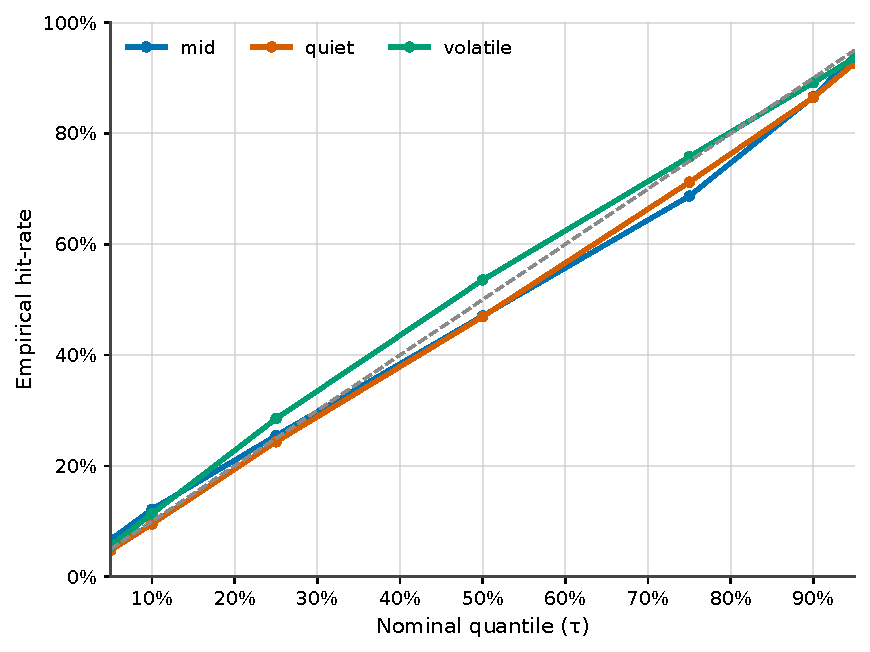
\includegraphics[width=0.7\linewidth,height=\textheight,keepaspectratio]{appendices/figures/final/fig-qrf-v3-reliability-by-regime.pdf}

}

\caption{\label{fig-qrf-v3-reliability-by-regime}QRF v3 reliability by
regime; each line shows empirical hit-rate vs nominal τ for a regime;
ideal line shown.}

\end{figure}%

\begin{figure}

\centering{

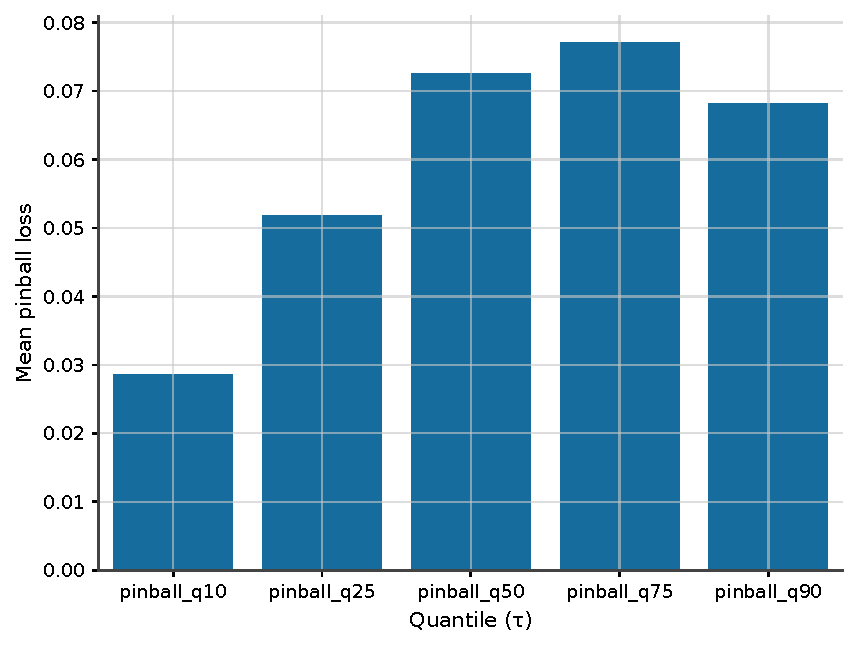
\includegraphics[width=0.62\linewidth,height=\textheight,keepaspectratio]{appendices/figures/final/fig-qrf-v1-pinball-mean.pdf}

}

\caption{\label{fig-qrf-v1-pinball-mean}QRF v1 mean pinball loss per
quantile.}

\end{figure}%

\textbf{QRF implementation notes \{\#app-r4-qrf-code\}}

See Appendix 5 for full Model code

\textbf{QRF variants and hyper‑parameters \{\#app-t3-qrf-hparams\}}

This section collects the hyper‑parameter search ranges, final values
and variant metrics for the Quantile Regression Forest (QRF) models
referenced in Chapter~4. Use this table to reproduce the model
specifications and to understand the trade‑offs explored in the
robustness checks.

\textbf{Table 1}

\begin{longtable}[]{@{}ll@{}}
\toprule\noalign{}
Parameter & Value \\
\midrule\noalign{}
\endhead
\bottomrule\noalign{}
\endlastfoot
n\_estimators & 1467 \\
max\_depth & 24 \\
min\_samples\_leaf & 5 \\
max\_features\_choice & fraction \\
max\_features & 0.9984302781608038 \\
\end{longtable}

\begin{center}\rule{0.5\linewidth}{0.5pt}\end{center}

\textbf{Linear Quantile Regression optimisation \{\#app-l1-lqr\}}

\textbf{Problem statement.} For each quantile level \(\tau\) and feature
vector \(x\), LQR solves

\[
\widehat{\beta}_{\tau} = \arg\min_{\beta\in \mathbb{R}^{p+1}} \sum_{t\in\mathcal{T}_{\text{train}}} \rho_{\tau}\big( y_{t} - [1,x_{t}]^{\top}\beta \big),
\quad
\widehat q_{\tau}(x) = [1,x]^{\top} \widehat{\beta}_{\tau}.
\]

The pinball loss \(\rho_{\tau}\) is defined in Appendix~M1. Each
\(\tau\) is fit independently.

\textbf{Design notes.} Numeric predictors are standardised using
training statistics; categorical variables are one‑hot encoded with an
intercept. No further transformations are applied. Convergence and
solver settings for \texttt{statsmodels.QuantReg} are summarised below.

\begin{figure}

\centering{

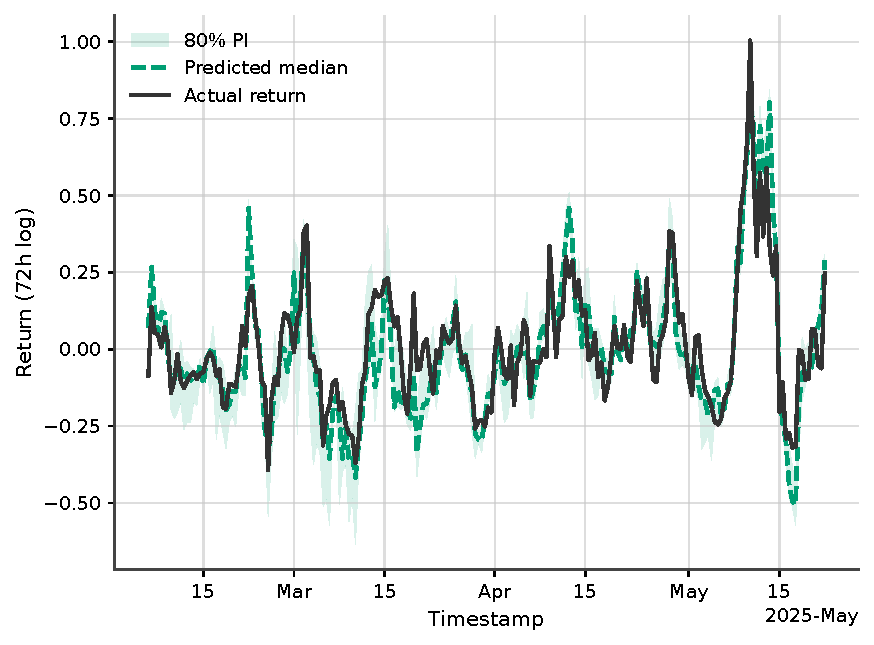
\includegraphics[width=0.72\linewidth,height=\textheight,keepaspectratio]{appendices/figures/final/fig-lqr-fan-longest.pdf}

}

\caption{\label{fig-lqr-fan-longest}Linear-QR 72-hour forecast fan chart
for the token BOME.}

\end{figure}%

\begin{figure}

\centering{

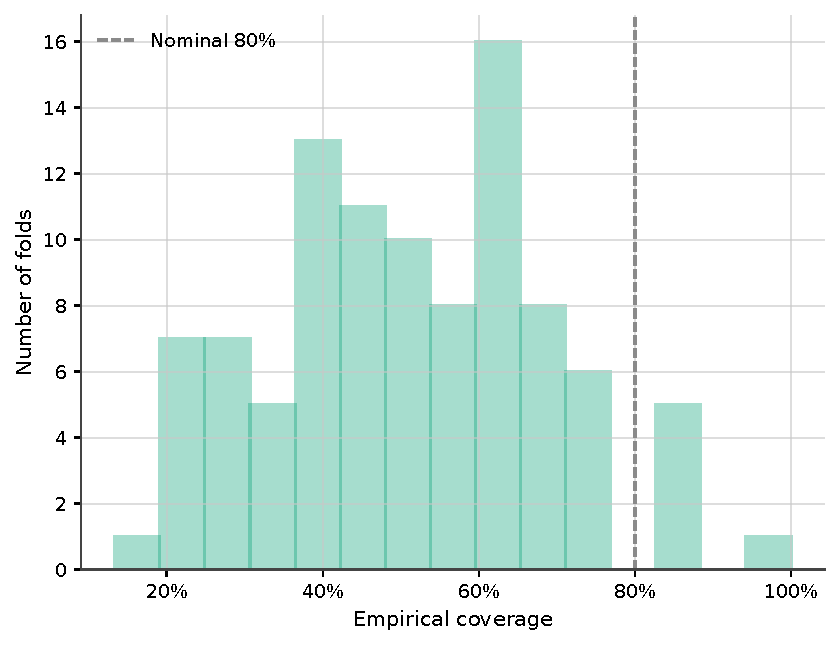
\includegraphics[width=0.62\linewidth,height=\textheight,keepaspectratio]{appendices/figures/final/fig-lqr-coverage-80pi-hist.pdf}

}

\caption{\label{fig-lqr-coverage-80pi-hist}Coverage of 80\% prediction
intervals across folds; dashed line marks nominal 80\%.}

\end{figure}%

\begin{figure}

\centering{

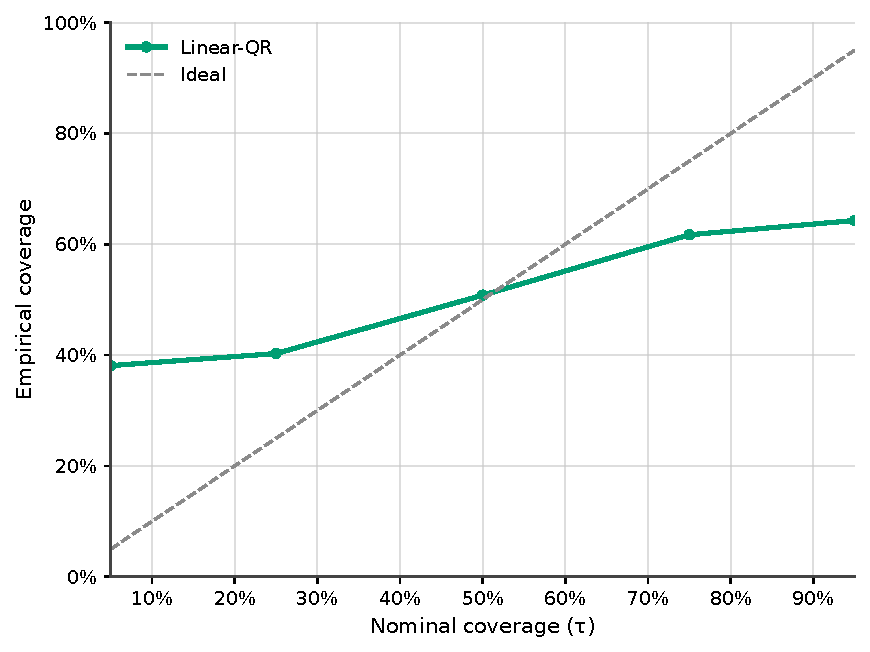
\includegraphics[width=0.64\linewidth,height=\textheight,keepaspectratio]{appendices/figures/final/fig-lqr-v1-calibration.pdf}

}

\caption{\label{fig-lqr-calibration}Linear-QR calibration: empirical vs
nominal coverage (ideal line shown).}

\end{figure}%

\begin{center}\rule{0.5\linewidth}{0.5pt}\end{center}

\textbf{LightGBM quantile objective and boosting \{\#app-g1-lgbm-obj\}}

\textbf{Boosting update.} Let \(F_m^{(\tau)}(x)\) denote the stage‑\(m\)
prediction for quantile level \(\tau\). Gradient boosting updates via

\[
F_{m}^{(\tau)}(x) = F_{m-1}^{(\tau)}(x) + \eta\, f_{m}^{(\tau)}(x),
\]

where \(f_{m}^{(\tau)}\) is a regression tree and \(\eta\in(0,1]\) is
the learning rate.

\textbf{Negative gradient for the pinball loss.} For residual
\(u_t = y_t - F_{m-1}^{(\tau)}(x_t)\),

\[
 g_{t}^{(\tau)} = -\frac{\partial}{\partial \hat y}\,\rho_{\tau}(u_t)\Big|_{\hat y = F_{m-1}^{(\tau)}(x_t)} = \tau - \mathbf{1}\{ y_t < F_{m-1}^{(\tau)}(x_t) \}.
\]

LightGBM fits \(f_{m}^{(\tau)}\) to \((x_t,g_t^{(\tau)})\) using
histogram‑based splits and leaf‑wise growth; second‑order terms vanish
for the pinball loss, so a first‑order update suffices.

\textbf{Table 2 --- LightGBM hyper‑parameters by quantile
\{\#app-t2-lgbm-hparams\}}

\begin{longtable}[]{@{}
  >{\centering\arraybackslash}p{(\linewidth - 22\tabcolsep) * \real{0.0556}}
  >{\raggedright\arraybackslash}p{(\linewidth - 22\tabcolsep) * \real{0.0833}}
  >{\raggedleft\arraybackslash}p{(\linewidth - 22\tabcolsep) * \real{0.0648}}
  >{\raggedleft\arraybackslash}p{(\linewidth - 22\tabcolsep) * \real{0.0648}}
  >{\raggedleft\arraybackslash}p{(\linewidth - 22\tabcolsep) * \real{0.0926}}
  >{\raggedleft\arraybackslash}p{(\linewidth - 22\tabcolsep) * \real{0.1019}}
  >{\raggedleft\arraybackslash}p{(\linewidth - 22\tabcolsep) * \real{0.0926}}
  >{\raggedleft\arraybackslash}p{(\linewidth - 22\tabcolsep) * \real{0.0926}}
  >{\raggedleft\arraybackslash}p{(\linewidth - 22\tabcolsep) * \real{0.1111}}
  >{\raggedleft\arraybackslash}p{(\linewidth - 22\tabcolsep) * \real{0.1111}}
  >{\raggedleft\arraybackslash}p{(\linewidth - 22\tabcolsep) * \real{0.0648}}
  >{\raggedleft\arraybackslash}p{(\linewidth - 22\tabcolsep) * \real{0.0648}}@{}}
\toprule\noalign{}
\begin{minipage}[b]{\linewidth}\centering
τ
\end{minipage} & \begin{minipage}[b]{\linewidth}\raggedright
lr
\end{minipage} & \begin{minipage}[b]{\linewidth}\raggedleft
leaves
\end{minipage} & \begin{minipage}[b]{\linewidth}\raggedleft
depth
\end{minipage} & \begin{minipage}[b]{\linewidth}\raggedleft
min\_leaf
\end{minipage} & \begin{minipage}[b]{\linewidth}\raggedleft
feat\_frac
\end{minipage} & \begin{minipage}[b]{\linewidth}\raggedleft
bag\_frac
\end{minipage} & \begin{minipage}[b]{\linewidth}\raggedleft
bag\_freq
\end{minipage} & \begin{minipage}[b]{\linewidth}\raggedleft
L1
\end{minipage} & \begin{minipage}[b]{\linewidth}\raggedleft
L2
\end{minipage} & \begin{minipage}[b]{\linewidth}\raggedleft
gamma
\end{minipage} & \begin{minipage}[b]{\linewidth}\raggedleft
iters
\end{minipage} \\
\midrule\noalign{}
\endhead
\bottomrule\noalign{}
\endlastfoot
0.05 & 0.01078 & 253 & 4 & 96 & 0.762 & 0.711 & 4 & 8.15e-06 & 2.09e-07
& 0.069 & 2449 \\
0.10 & 0.00622 & 91 & 13 & 37 & 0.862 & 0.714 & 15 & 2.6940 & 0.5684 &
0.172 & 7495 \\
0.25 & 0.00783 & 42 & 6 & 79 & 0.622 & 0.963 & 11 & 0.01731 & 0.8099 &
0.085 & 7999 \\
0.50 & 0.01376 & 56 & 5 & 22 & 0.960 & 0.796 & 11 & 3.95e-06 & 3.85e-07
& 0.333 & 7992 \\
0.75 & 0.05456 & 68 & 9 & 76 & 0.520 & 0.994 & 1 & 5.21e-08 & 1.94e-04 &
0.060 & 1095 \\
0.90 & 0.04030 & 96 & 7 & 78 & 0.909 & 0.445 & 2 & 3.49e-05 & 3.41e-05 &
0.191 & 218 \\
0.95 & 0.00617 & 201 & 4 & 8 & 0.776 & 0.990 & 3 & 0.00117 & 4.83e-06 &
0.162 & 3200 \\
\end{longtable}

\begin{figure}

\centering{

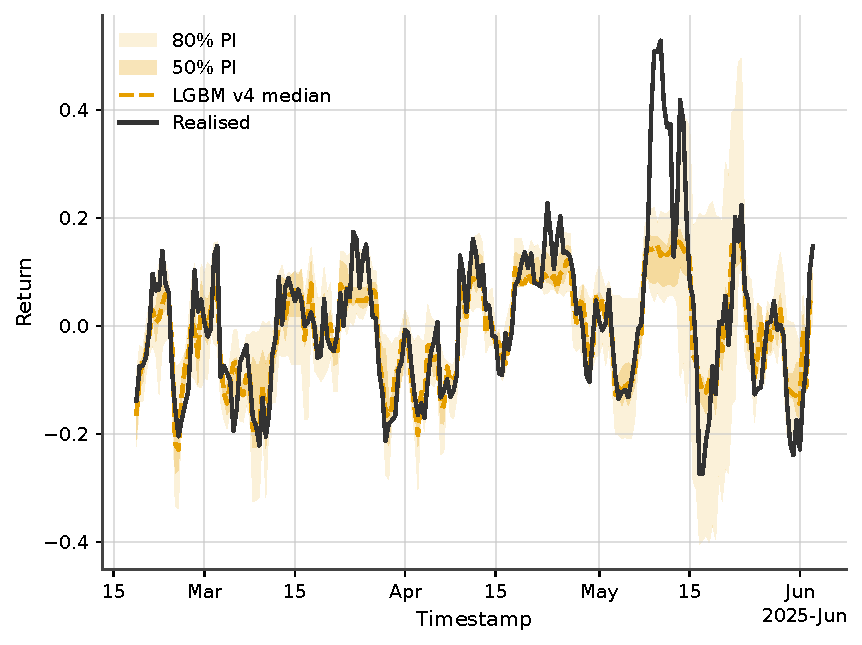
\includegraphics[width=0.72\linewidth,height=\textheight,keepaspectratio]{appendices/figures/final/fig-lgbm-v4-fan-bome.pdf}

}

\caption{\label{fig-lgbm-v4-fan-bome}LightGBM-CQR v4 fan chart with
central median and central interval around the median; realised series
overlaid. Compared to the V3 and V2, this shows the tightest intervals}

\end{figure}%

\begin{figure}

\centering{

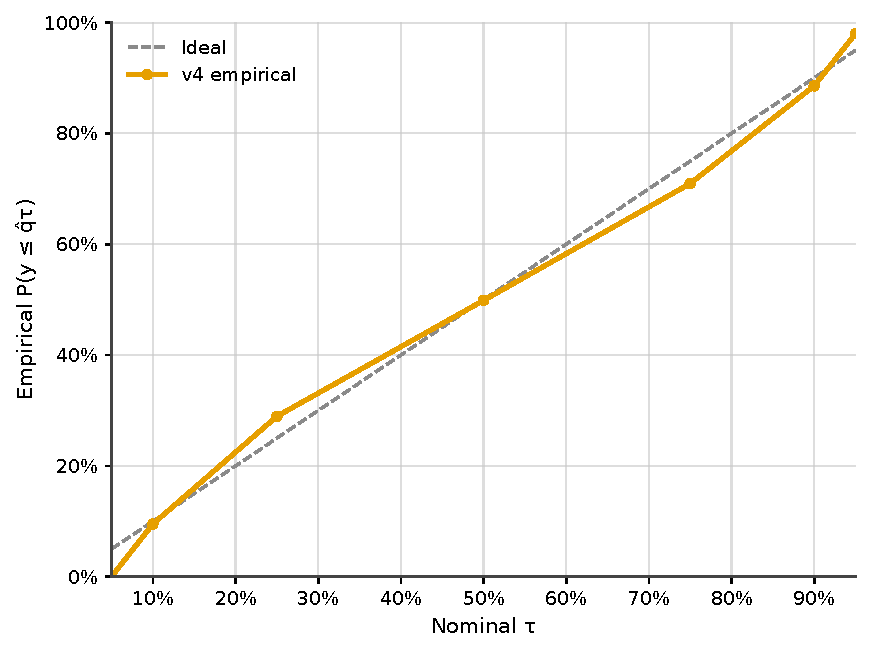
\includegraphics[width=0.64\linewidth,height=\textheight,keepaspectratio]{appendices/figures/final/fig-lgbm-v4-calibration.pdf}

}

\caption{\label{fig-lgbm-v4-calibration}Calibration of LightGBM-CQR v4:
empirical CDF hits vs nominal τ; ideal line shown.}

\end{figure}%

\textbf{See appendix 4 for all figures and tables related to QRF}

\begin{center}\rule{0.5\linewidth}{0.5pt}\end{center}

\subsection{Statistical tests}\label{app-m4-tests}

\textbf{C with HAC and HLN.} Let \(d_t\) be the loss differential (e.g.,
pinball) between models \(A\) and \(B\) at the same \(\tau\) on Test.
With \(\bar d=\tfrac{1}{T}\sum_t d_t\) and Bartlett-weighted Newey--West
spectral estimate \[
\widehat S_L \;=\; \widehat\gamma_0 + 2\sum_{\ell=1}^{L}\left(1-\frac{\ell}{L+1}\right)\widehat\gamma_\ell,
\qquad
\widehat\gamma_\ell=\frac{1}{T}\sum_{t=\ell+1}^{T}(d_t-\bar d)(d_{t-\ell}-\bar d),
\] the DM statistic is \[
\mathrm{DM} \;=\; \frac{\bar d}{\sqrt{\widehat S_L/T}}.
\] Small-sample \textbf{Harvey--Leybourne--Newbold (HLN)} correction is
applied to obtain \(p\)-values. Two-sided tests are used throughout.

\textbf{Multiplicity.} Across multiple \(\tau\) we control the false
discovery rate with \textbf{Benjamini--Hochberg} at level \(q\): sort
p-values \(p_{(1)}\le\cdots\le p_{(m)}\) and reject up to
\(k=\max\{i: p_{(i)}\le (i/m)q\}\). Holm--Bonferroni adjusted p-values
are also reported.

\textbf{The Model Confidence Set}

The Model Confidence Set is an iterative, bootstrap-based procedure that
tests the null of \textbf{Equal Predictive Ability} across models and
sequentially removes the worst performer until the null cannot be
rejected, yielding a \textbf{superior set} at confidence level
\(1-\alpha\). It controls for multiple comparisons and model-selection
uncertainty, so instead of declaring a single ``winner'' it returns a
statistically validated set; we apply it to rolling
\textbf{pinball-loss} series across models and quantiles.

\begin{center}\rule{0.5\linewidth}{0.5pt}\end{center}

\subsection{Metric definitions}\label{app-m5-metrics}

\textbf{Coverage and width.} For a central \((1-\alpha)\) interval
\([L_t,U_t]\) on a Test window of length \(T\), define

\[
\widehat{\mathrm{cov}} = \frac{1}{T} \sum_{t=1}^{T} \mathbf{1}\{ L_t \le y_t \le U_t \},
\qquad
\overline{\mathrm{width}} = \frac{1}{T} \sum_{t=1}^{T} (U_t - L_t).
\]

We also report the \textbf{coverage error}
\(|\widehat{\mathrm{cov}} - (1-\alpha)|\) and \textbf{conditional
coverage} by deciles of predicted width.

\textbf{Quantile reliability.} The empirical hit‑rate at quantile level
\(\tau\) is

\[
\widehat F_{\tau} = \frac{1}{T} \sum_{t=1}^{T} \mathbf{1}\{ y_t \le \widehat q_{\tau}(x_t) \}.
\] Perfect calibration corresponds to \(\widehat F_{\tau} = \tau\) for
all \(\tau\).

\textbf{Interval score} For a central interval \([L_t,U_t]\) with
nominal coverage \(1-\alpha\) and observation \(y_t\), the interval
score (Gneiting~\&~Raftery, 2007) is

\[
S_{\alpha}(L_t,U_t;y_t) = (U_t-L_t) + \frac{2}{\alpha} (L_t - y_t)\,\mathbf{1}\{ y_t < L_t \} + \frac{2}{\alpha} (y_t - U_t)\,\mathbf{1}\{ y_t > U_t \}.
\] Lower values indicate sharper, better‑calibrated intervals.

\begin{center}\rule{0.5\linewidth}{0.5pt}\end{center}

\textbf{Table 3}

\begin{longtable}[]{@{}
  >{\raggedright\arraybackslash}p{(\linewidth - 4\tabcolsep) * \real{0.1342}}
  >{\raggedright\arraybackslash}p{(\linewidth - 4\tabcolsep) * \real{0.6779}}
  >{\raggedright\arraybackslash}p{(\linewidth - 4\tabcolsep) * \real{0.1879}}@{}}
\toprule\noalign{}
\begin{minipage}[b]{\linewidth}\raggedright
Metric
\end{minipage} & \begin{minipage}[b]{\linewidth}\raggedright
Definition (short)
\end{minipage} & \begin{minipage}[b]{\linewidth}\raggedright
Notes
\end{minipage} \\
\midrule\noalign{}
\endhead
\bottomrule\noalign{}
\endlastfoot
Pinball loss &
\(\rho_{\tau}(u)=u\big(\tau-\mathbf{1}\{u<0\}\big),\; u=y-\widehat q_{\tau}(x)\)
& Per-\(\tau\); mean over \(\mathcal T\) \\
Coverage &
\(\widehat{\mathrm{cov}}=\tfrac{1}{T}\sum_{t=1}^{T}\mathbf{1}\{L_t\le y_t\le U_t\}\)
& Target \(1-\alpha\) \\
Width &
\(\overline{\mathrm{width}}=\tfrac{1}{T}\sum_{t=1}^{T}(U_t-L_t)\) & Pair
with coverage \\
Coverage error & \(\lvert \widehat{\mathrm{cov}}-(1-\alpha)\rvert\) &
Lower is better \\
Reliability &
\(\widehat F_{\tau}=\tfrac{1}{T}\sum_{t=1}^{T}\mathbf{1}\{y_t\le \widehat q_{\tau}(x_t)\}\)
& Plot \(\widehat F_{\tau}\) vs \(\tau\) \\
Interval score &
\(S_{\alpha}=(U-L)+\tfrac{2}{\alpha}(L-y)\mathbf{1}\{y<L\}+\tfrac{2}{\alpha}(y-U)\mathbf{1}\{y>U\}\)
& Optional \\
\end{longtable}

This table summarises the metrics referenced in the Methods and Results
chapters. See the definitions above and
\textbf{Appendix~(\citeproc{ref-ref}{\textbf{ref?}})(app-m5-metrics)}
for derivations.

\begin{center}\rule{0.5\linewidth}{0.5pt}\end{center}

\textbf{Table 4: Feature dictionary (full list of predictors)
\{\#app-fdict\}}

Table~\texttt{@tbl-used-features} lists the complete set of features
used in the modelling (feature‑set~v1). Each row gives the variable
name, a brief description, and its family. Use this as a reference when
processing raw data and interpreting model coefficients.

\begin{longtable}[]{@{}
  >{\raggedright\arraybackslash}p{(\linewidth - 6\tabcolsep) * \real{0.3247}}
  >{\raggedright\arraybackslash}p{(\linewidth - 6\tabcolsep) * \real{0.2597}}
  >{\centering\arraybackslash}p{(\linewidth - 6\tabcolsep) * \real{0.0779}}
  >{\raggedright\arraybackslash}p{(\linewidth - 6\tabcolsep) * \real{0.3377}}@{}}
\toprule\noalign{}
\begin{minipage}[b]{\linewidth}\raggedright
Family
\end{minipage} & \begin{minipage}[b]{\linewidth}\raggedright
Feature Name
\end{minipage} & \begin{minipage}[b]{\linewidth}\centering
Window
\end{minipage} & \begin{minipage}[b]{\linewidth}\raggedright
Description
\end{minipage} \\
\midrule\noalign{}
\endhead
\bottomrule\noalign{}
\endlastfoot
\textbf{Momentum} & \texttt{logret\_12h} & 1 & 12-hour log return. \\
& \texttt{logret\_36h} & 3 & 36-hour log return. \\
& \texttt{proc} & -- & Price rate of change. \\
& \texttt{rsi\_14} & 14 & Relative Strength Index. \\
& \texttt{stoch\_k} & 14 & Stochastic \%K. \\
& \texttt{cci} & -- & Commodity Channel Index. \\
& \texttt{macd} & 12/26 & MACD (fast/slow EMA diff). \\
& \texttt{macd\_signal} & 9 & MACD signal line. \\
\textbf{Volatility} & \texttt{realized\_vol\_36h} & 3 & Std. of
\texttt{logret\_12h}. \\
& \texttt{vol\_std\_7bar} & 7 & Rolling return std. \\
& \texttt{downside\_vol\_3bar} & 3 & Std. of negative returns. \\
& \texttt{parkinson\_vol\_36h} & 3 & Parkinson high--low vol. \\
& \texttt{gk\_vol\_36h} & 3 & Garman--Klass vol. \\
& \texttt{atr\_14} & 14 & Average True Range. \\
& \texttt{bollinger\_bw} & 20 & Bollinger band width. \\
& \texttt{bollinger\_b} & 20 & Bollinger \%B. \\
& \texttt{rolling\_skew\_50} & 50 & Skewness of returns. \\
& \texttt{skew\_36h} & 3 & 36-hour return skewness. \\
& \texttt{adx} & -- & Average Directional Index. \\
\textbf{Liquidity / Volume} & \texttt{amihud\_illiq\_12h} & 3 & Amihud
illiquidity (36h). \\
& \texttt{vol\_zscore\_14} & 14 & Volume z-score. \\
& \texttt{obv} & -- & On-Balance Volume. \\
\textbf{On-Chain} & \texttt{holder\_growth\_1bar} & 1 & \% change in
holders. \\
& \texttt{holder\_growth\_7d} & 14 & 7-day holder growth. \\
& \texttt{tx\_per\_account} & -- & Tx per active holder. \\
\textbf{Cross-Asset / Context} & \texttt{ret\_SOL} & 1 & SOL 12-h
return. \\
& \texttt{ret\_ETH} & 1 & ETH 12-h return. \\
& \texttt{ret\_BTC} & 1 & BTC 12-h return. \\
& \texttt{sol\_return} & 1 & SOL 12-h log return. \\
& \texttt{corr\_SOL\_36h} & 3 & Corr. to SOL returns. \\
\textbf{Calendar / Time} & \texttt{day\_of\_week} & -- & Categorical
(0--6). \\
& \texttt{hour\_cos} & -- & Cyclical hour encoding. \\
\textbf{Tail / Regime markers} & \texttt{extreme\_flag1} & -- &
Extreme-move indicator. \\
& \texttt{extreme\_count\_72h} & 6 & \# extremes in past 72h. \\
& \texttt{tail\_asym} & -- & Tail asymmetry score. \\
& \texttt{vol\_regime} & -- & Quiet / volatile tag. \\
\end{longtable}

\chapter{Appendix 3: Results, Plots and Tables}\label{app-r1}

\textbf{Overall accuracy and Calibration}

\begin{figure}

\centering{

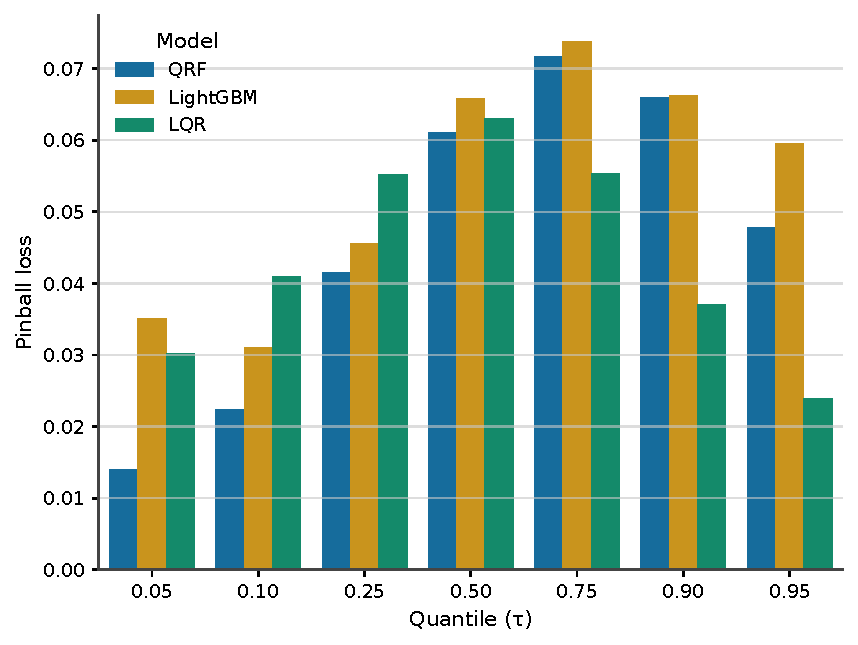
\includegraphics[width=0.64\linewidth,height=\textheight,keepaspectratio]{appendices/figures/final/fig-pinball-by-quantile-by-model.pdf}

}

\caption{\label{fig-pinball-by-quantile-by-model}Pinball loss by model
and quantile.}

\end{figure}%

\begin{figure}

\centering{

\includegraphics[width=0.7\linewidth,height=\textheight,keepaspectratio]{appendices/figures/final/fig-pinball-per-token.pdf}

}

\caption{\label{fig-pinball-per-token}Per-token pinball loss by model
and quantile; boxes show dispersion across tokens, diamonds mark
per-quantile means.}

\end{figure}%

\begin{figure}

\centering{

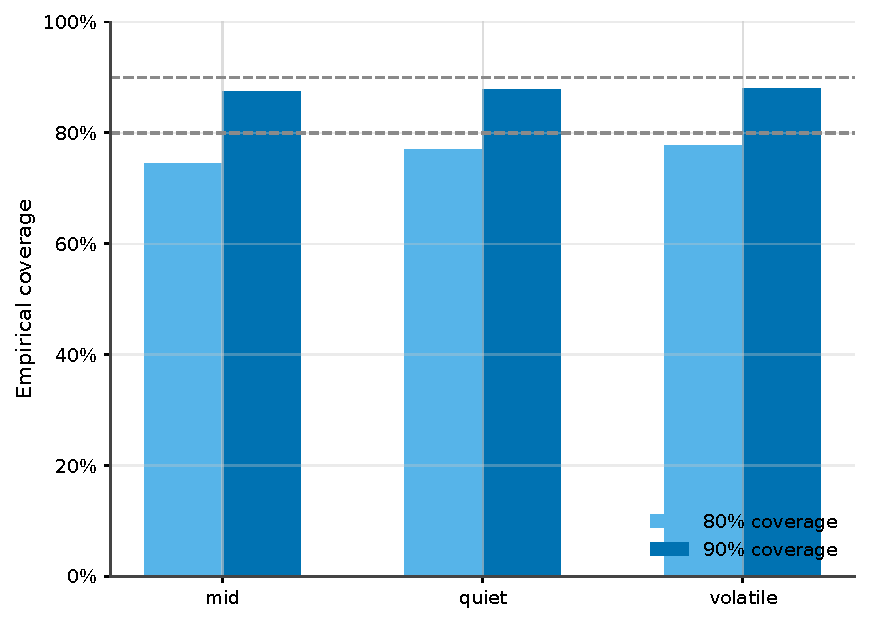
\includegraphics[width=0.62\linewidth,height=\textheight,keepaspectratio]{appendices/figures/final/fig-qrf-reliability-by-regime-bars.pdf}

}

\caption{\label{fig-qrf-reliability-by-regime-bars}QRF empirical
coverage by volatility regime for 80\% and 90\% intervals; dashed lines
mark nominal coverage.}

\end{figure}%

\begin{figure}

\centering{

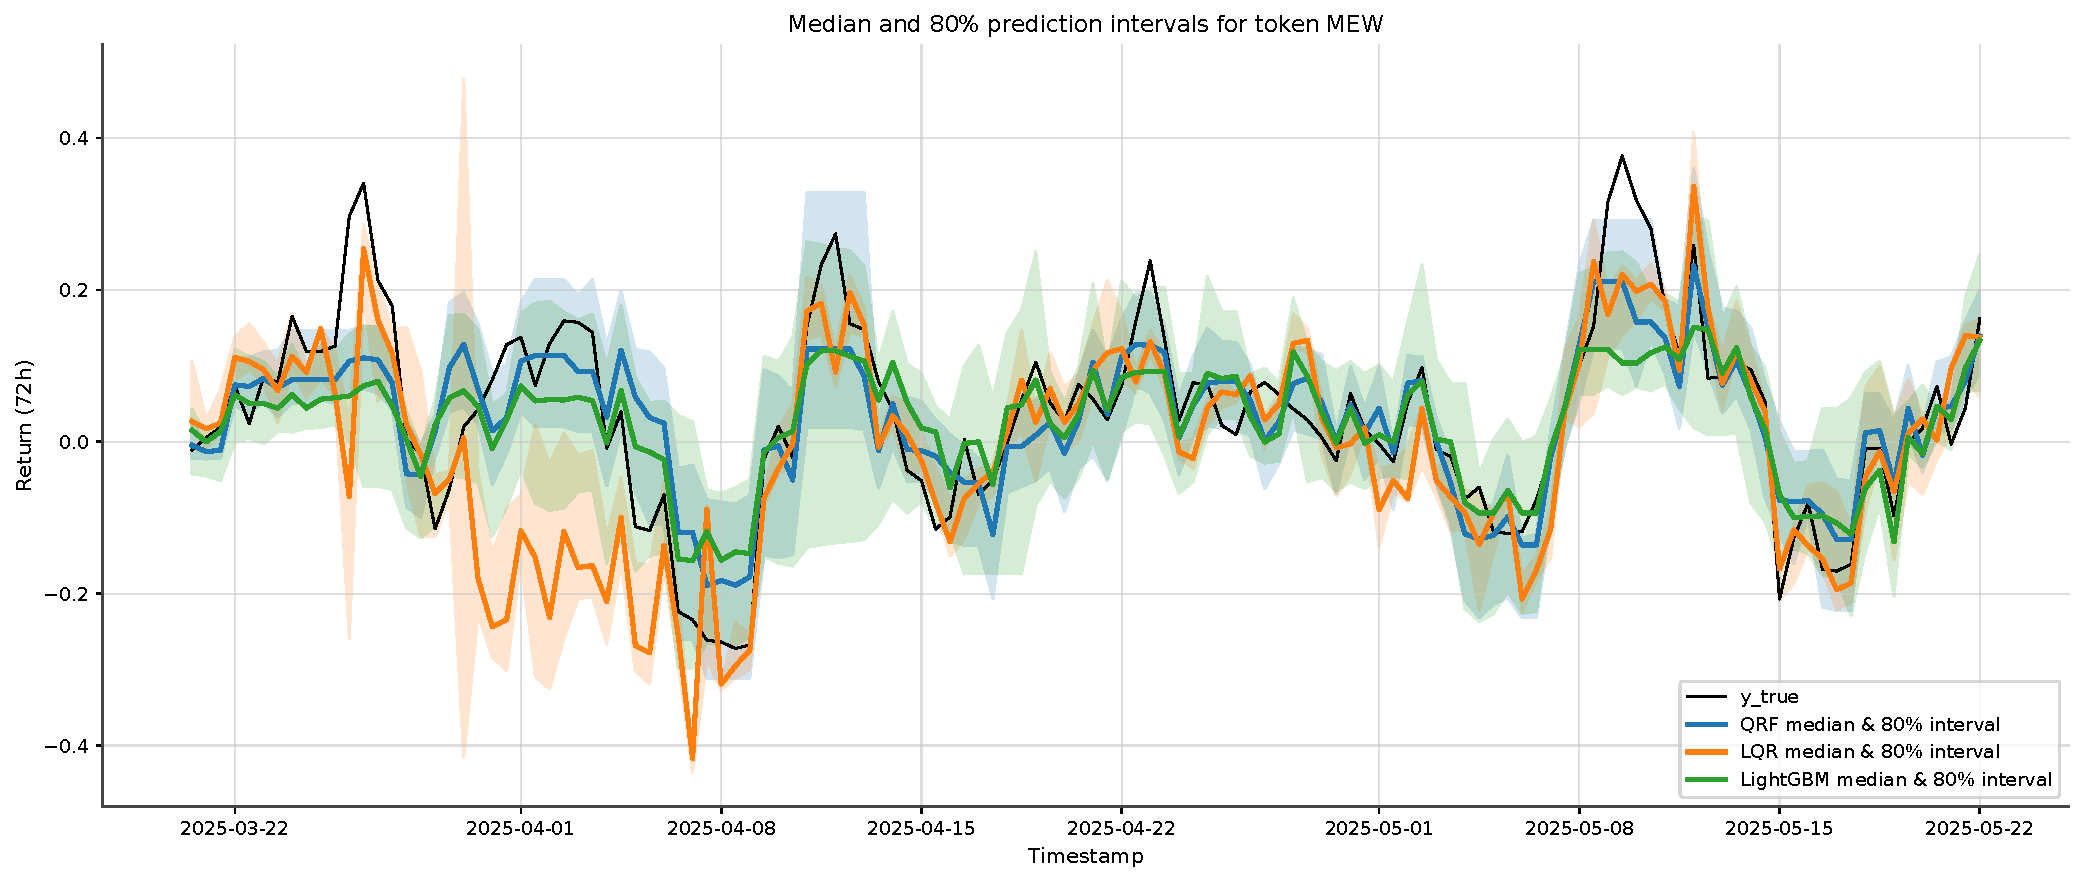
\includegraphics[width=0.72\linewidth,height=\textheight,keepaspectratio]{appendices/figures/final/fig-mew-80preds.pdf}

}

\caption{\label{fig-compare-80preds}Median and 80\% prediction intervals
for QRF, LQR, and LightGBM on the same token; realised series overlaid.}

\end{figure}%

\begin{figure}

\centering{

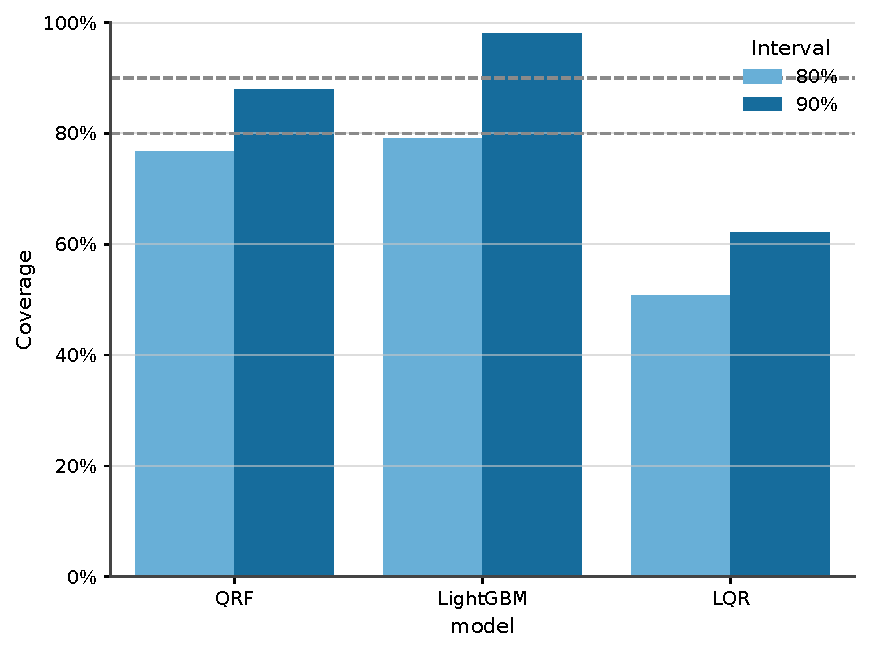
\includegraphics[width=0.64\linewidth,height=\textheight,keepaspectratio]{appendices/figures/final/fig-coverage-by-model.pdf}

}

\caption{\label{fig-coverage-by-model}Coverage of 80\% and 90\%
prediction intervals by model; dashed lines mark nominal levels.}

\end{figure}%

\phantomsection\label{fig-widths}\href{paper/figures/raw/fig-width-distributions.pdf}{Model
Widths}

\textbf{Table: Coverage by Regime:}

\begin{longtable}[]{@{}cccc@{}}
\toprule\noalign{}
regime & w80\_decile & coverage80 & n \\
\midrule\noalign{}
\endhead
\bottomrule\noalign{}
\endlastfoot
mid & 1 & 0.318 & 44 \\
mid & 5 & 0.793 & 111 \\
mid & 10 & 0.893 & 28 \\
quiet & 6 & 0.871 & 139 \\
quiet & 8 & 0.964 & 83 \\
quiet & 10 & 0.944 & 18 \\
volatile & 1 & 0.182 & 22 \\
volatile & 5 & 0.709 & 55 \\
volatile & 10 & 0.821 & 280 \\
\end{longtable}

\chapter{Appendix 4: Extras}\label{appendix-4-extras}

\textbf{Software and environment \{\#app-r1-software\}} \emph{Software
packages and versions.}

\begin{longtable}[]{@{}
  >{\raggedright\arraybackslash}p{(\linewidth - 4\tabcolsep) * \real{0.1673}}
  >{\raggedleft\arraybackslash}p{(\linewidth - 4\tabcolsep) * \real{0.0456}}
  >{\raggedright\arraybackslash}p{(\linewidth - 4\tabcolsep) * \real{0.7871}}@{}}
\toprule\noalign{}
\begin{minipage}[b]{\linewidth}\raggedright
Package / module
\end{minipage} & \begin{minipage}[b]{\linewidth}\raggedleft
Version
\end{minipage} & \begin{minipage}[b]{\linewidth}\raggedright
Purpose / notes
\end{minipage} \\
\midrule\noalign{}
\endhead
\bottomrule\noalign{}
\endlastfoot
\textbf{statsmodels} & 0.14.0 & Used \texttt{statsmodels.QuantReg} to
fit the Linear Quantile Regression (LQR) baseline. \\
\textbf{lightgbm} & 3.3.5 & Implements gradient‑boosted trees with a
quantile (pinball) loss for the LightGBM baseline; tuned via Optuna;
deterministic settings enabled. \\
\textbf{quantile‑forest} & 1.4.0 & Provides
\texttt{RandomForestQuantileRegressor} used for the Quantile Regression
Forest (QRF) core model. \\
\textbf{numpy} & 1.26.4 & Core numerical array library; underpinning of
all preprocessing and model computations. \\
\textbf{pandas} & 1.5.3 & Data ingestion and cleaning; assembling
12‑hour bar data, on‑chain metrics, and features. \\
\textbf{scikit‑learn} & 1.7.1 & General ML utilities; used indirectly
via LightGBM integration and for splitting data during hyperparameter
tuning. \\
\textbf{scipy} & 1.11.4 & Statistical functions (e.g.~Newey--West HAC
variance in DM tests) and optimisation routines. \\
\textbf{optuna} & 3.6.0 & Hyperparameter optimisation for LightGBM and
QRF models. \\
\textbf{optuna‑integration} & 4.4.0 & Integration helpers between Optuna
and LightGBM. \\
\textbf{properscoring} & 0.1 & Provides proper scoring rules such as
Continuous Ranked Probability Score (used for optional interval
scoring). \\
\textbf{dieboldmariano} & 1.1.0 & Facilitates Diebold--Mariano test
statistics used in model comparisons. \\
\textbf{arch} & 7.2.0 & Time‑series tools; potentially used for
volatility calculations or reference models. \\
\textbf{matplotlib} & 3.10.3 & Plotting calibration curves, fan charts,
and feature-importance visualisations. \\
\textbf{seaborn} & 0.13.2 & Statistical visualisation; sometimes used
alongside Matplotlib. \\
\textbf{joblib} & 1.5.1 & Parallel execution (e.g.~parallel fitting or
Optuna trials). \\
\textbf{requests} & 2.32.4 & Data ingestion via HTTP, such as fetching
12‑hour OHLCV bars and on‑chain metrics. \\
\textbf{python‑dotenv} & 1.1.1 & Loads API keys and environment
variables from \texttt{.env} files during data ingestion. \\
\textbf{nltk} (plus \texttt{SentimentIntensityAnalyzer}) & --- & Though
not in \texttt{pip\ freeze}, your ingestion scripts call
\texttt{nltk.sentiment.vader.SentimentIntensityAnalyzer} to compute
sentiment scores. You'd need to install \texttt{nltk} and download its
VADER lexicon separately. \\
\textbf{time}, \textbf{os} & --- (built‑in) & Standard library modules
for timing, delays, and file-system operations. \\
\end{longtable}

\section{Data Processing and EDA}\label{data-processing-and-eda}

\begin{figure}

\centering{

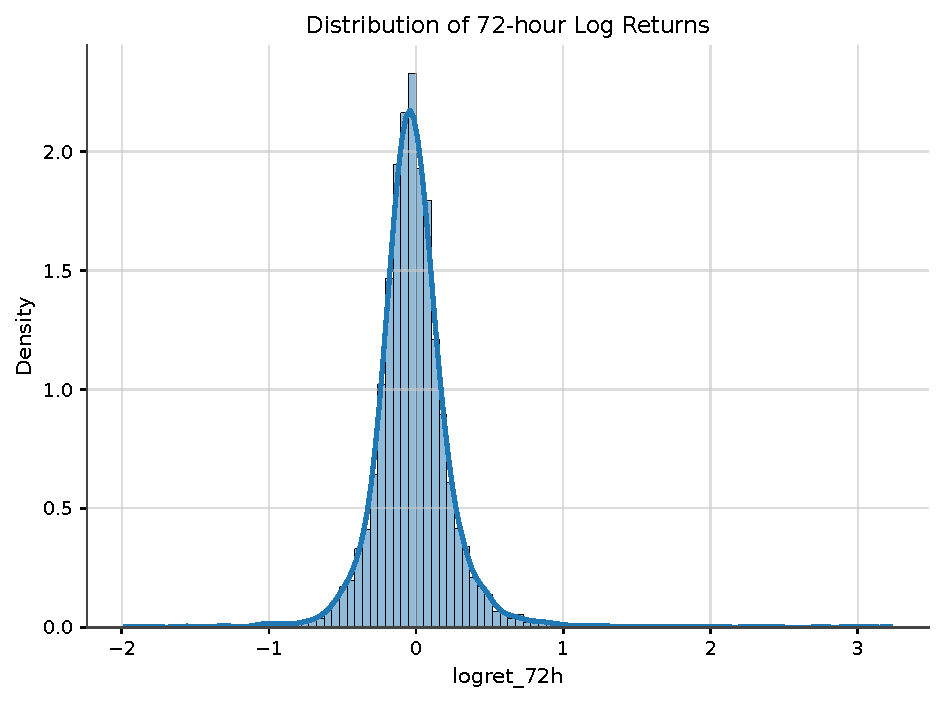
\includegraphics[width=0.65\linewidth,height=\textheight,keepaspectratio]{appendices/figures/raw/fig-3-1.pdf}

}

\caption{\label{fig-return-dist}Distribution of the 72-hour log return
target variable, pooled across all tokens. The distribution exhibits a
sharp peak and significantly heavier tails than a comparable normal
distribution, justifying the use of quantile-based models.}

\end{figure}%

Fig 1.1 --- OHLCV Missingness: before vs after cleaning
(Figure~\ref{fig-3-1-ohlcv-missingness}):

\begin{figure}

\centering{

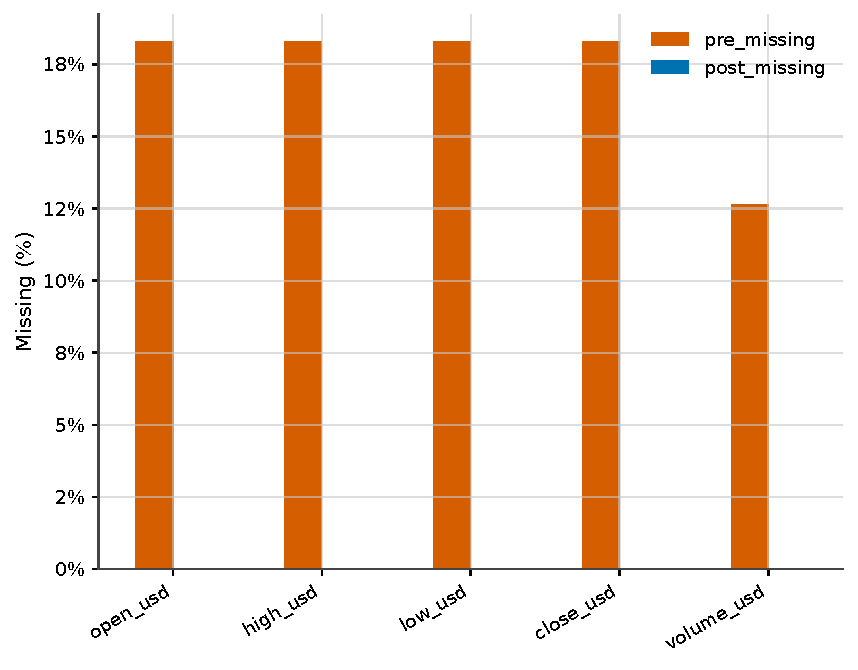
\includegraphics[width=0.62\linewidth,height=\textheight,keepaspectratio]{appendices/figures/final/fig-3-1-ohlcv-missingness.pdf}

}

\caption{\label{fig-3-1-ohlcv-missingness}Post-cleaning reduces
missingness across OHLCV fields; values shown as \% of rows.}

\end{figure}%

Fig 1.2 --- Missing holder\_count by token
(\textbf{?@fig-3-2-holder-missingness}):

\begin{center}
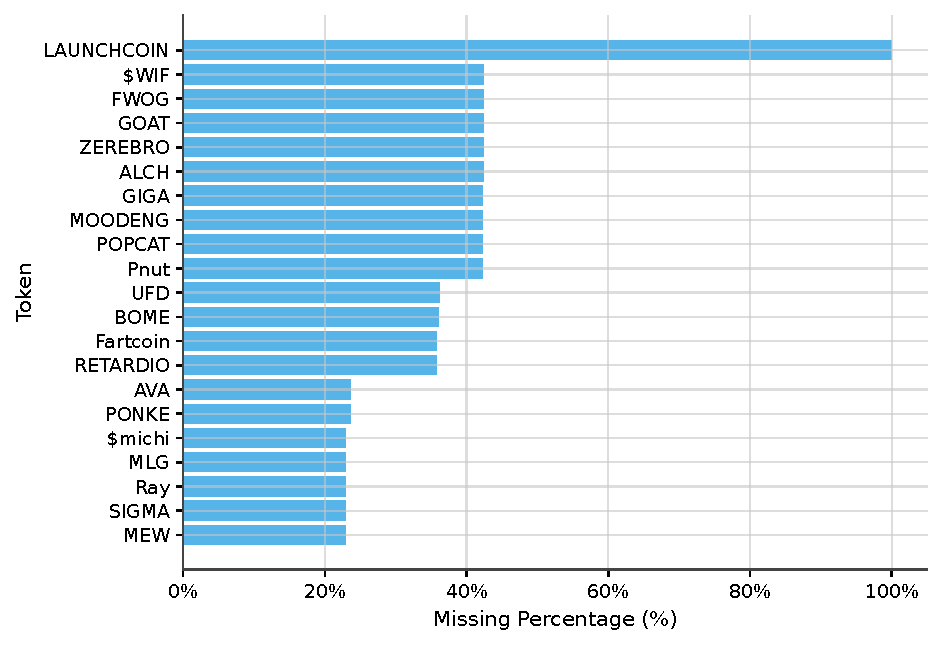
\includegraphics[width=0.62\linewidth,height=\textheight,keepaspectratio]{appendices/figures/final/fig-3-2-holder-missingness.pdf}
\end{center}
\}

Fig 1.3 --- Missing data per feature (without holder\_count)
(Figure~\ref{fig-3-3-missing-per-feature-no-holder}):

\begin{figure}

\centering{

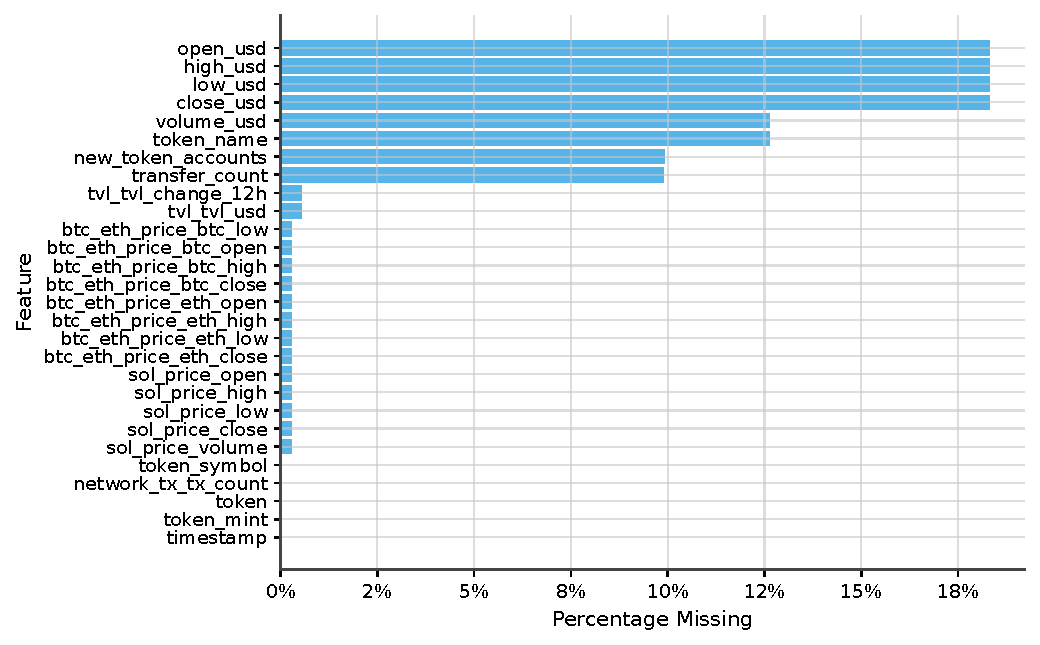
\includegraphics[width=0.64\linewidth,height=\textheight,keepaspectratio]{appendices/figures/final/fig-3-3-missing-per-feature-no-holder.pdf}

}

\caption{\label{fig-3-3-missing-per-feature-no-holder}Share of missing
values per variable before introducing holder\_count.}

\end{figure}%

Fig 1.4 --- Missing data per feature (post-2025-02-07)
(Figure~\ref{fig-3-4-missing-per-feature-post}):

\begin{figure}

\centering{

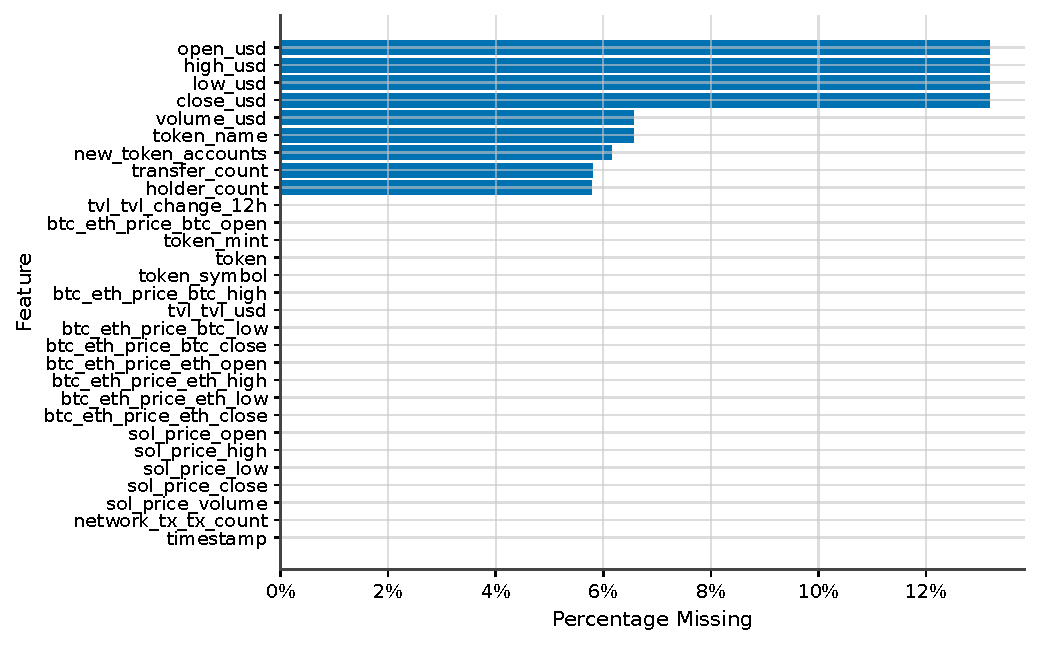
\includegraphics[width=0.64\linewidth,height=\textheight,keepaspectratio]{appendices/figures/final/fig-3-4-missing-per-feature-post.pdf}

}

\caption{\label{fig-3-4-missing-per-feature-post}Share of missing values
per variable after the 2025-02-07 boundary; includes holder\_count.}

\end{figure}%

Fig 3.5 --- Time-series missingness of OHLCV
(Figure~\ref{fig-3-5-timeseries-missingness-ohlcv}):

\begin{figure}

\centering{

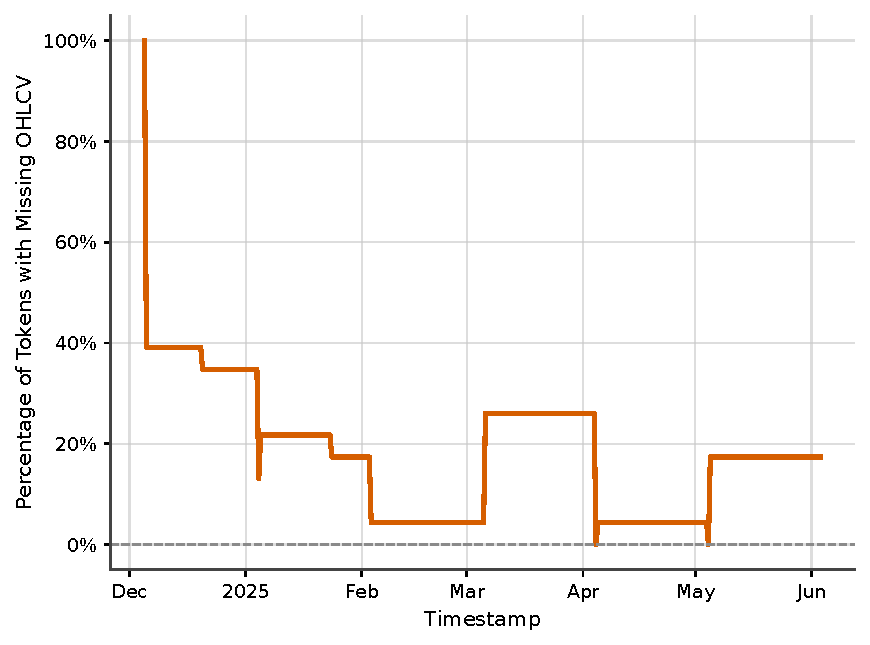
\includegraphics[width=0.68\linewidth,height=\textheight,keepaspectratio]{appendices/figures/final/fig-3-5-timeseries-missingness-ohlcv.pdf}

}

\caption{\label{fig-3-5-timeseries-missingness-ohlcv}Time-series share
of tokens with missing OHLCV values.}

\end{figure}%

\begin{figure}

\centering{

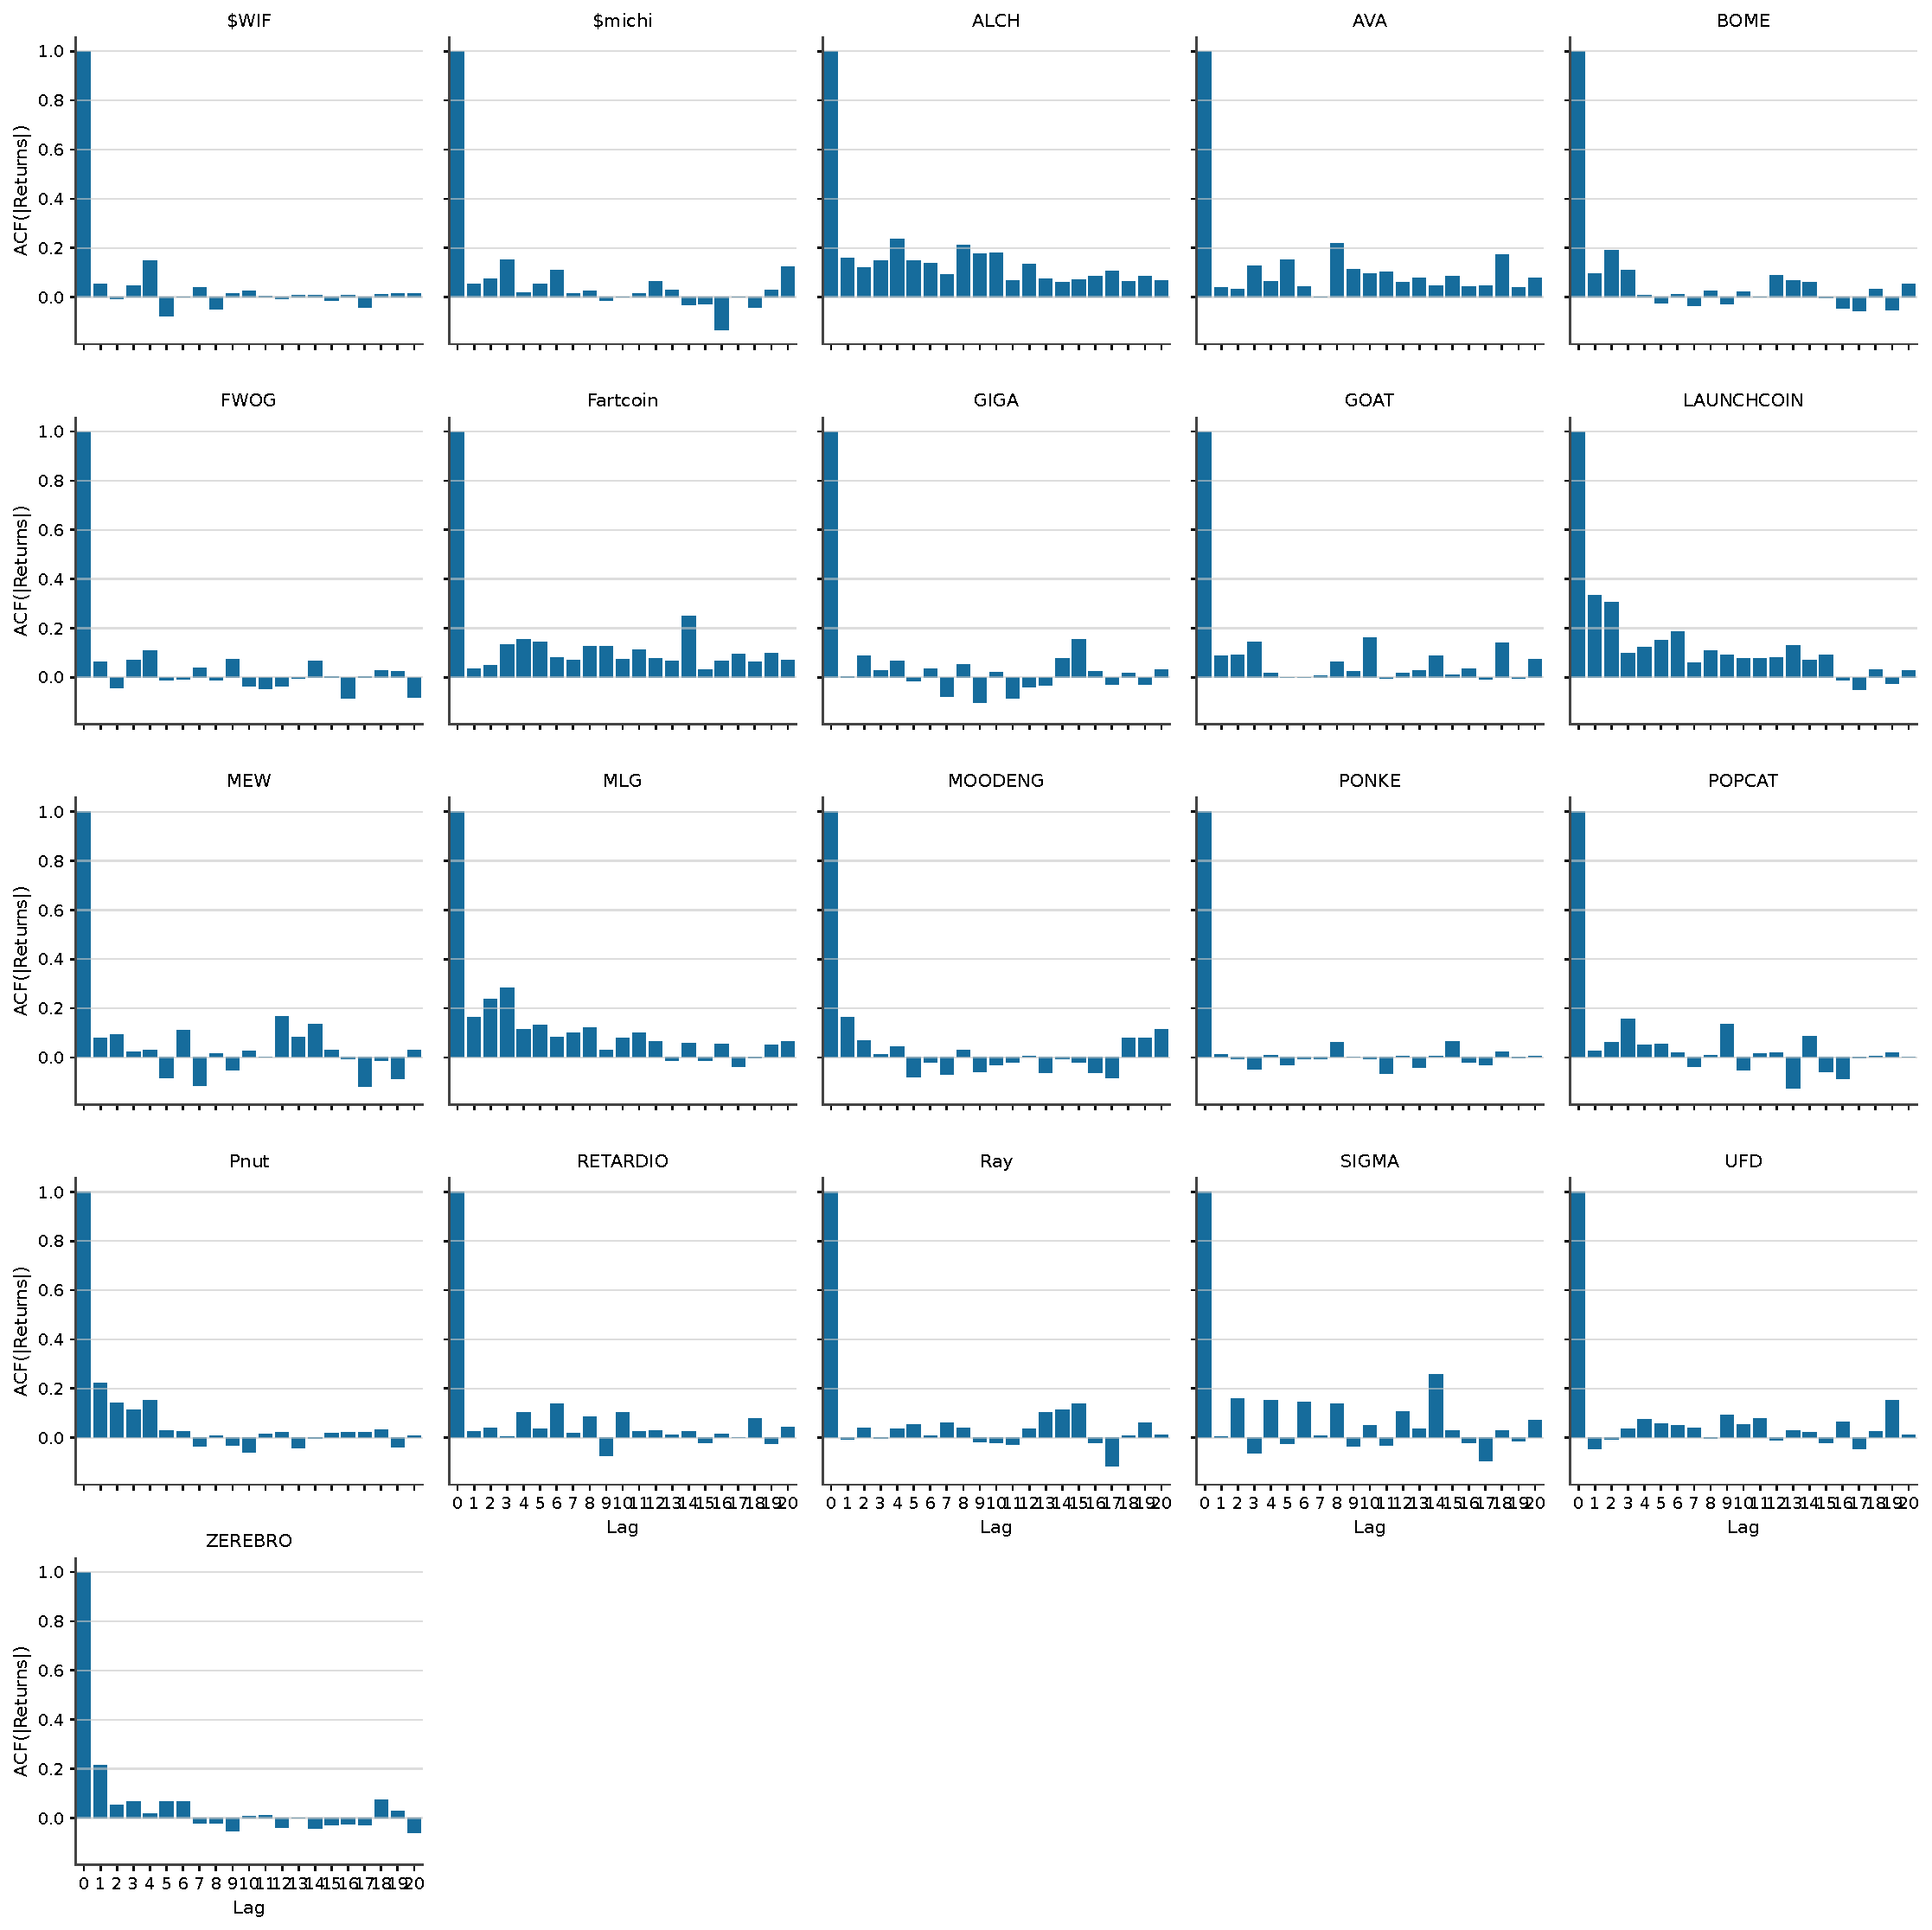
\includegraphics[width=0.72\linewidth,height=\textheight,keepaspectratio]{appendices/figures/final/fig-eda-acf-abs-12h.pdf}

}

\caption{\label{fig-acf-abs-returns}Per-token ACF of absolute 12h
returns (volatility clustering evident).}

\end{figure}%

\begin{figure}

\centering{

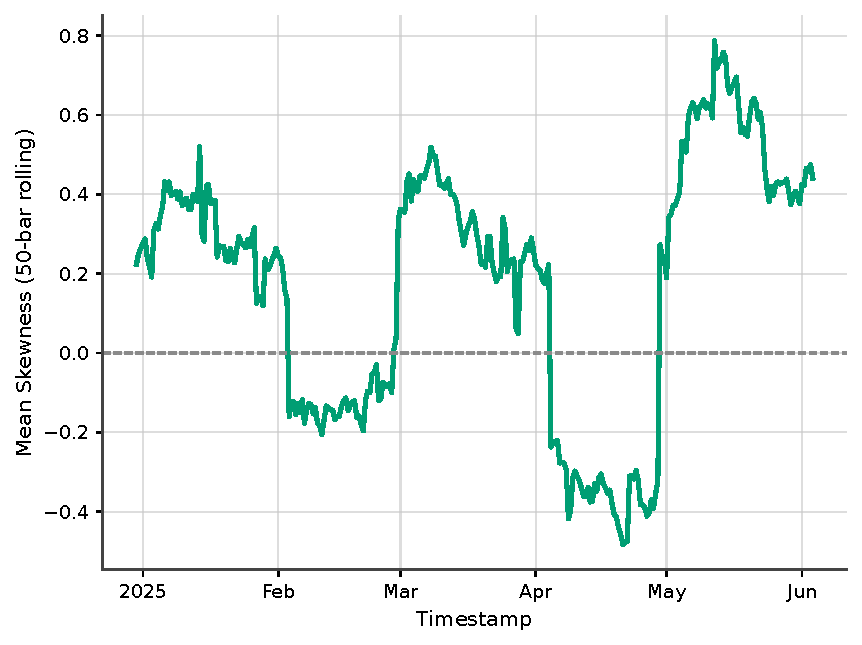
\includegraphics[width=0.64\linewidth,height=\textheight,keepaspectratio]{appendices/figures/final/fig-eda-rolling-skewness.pdf}

}

\caption{\label{fig-rolling-skewness}Panel-wide average rolling skewness
of 12h returns.}

\end{figure}%

\begin{figure}

\centering{

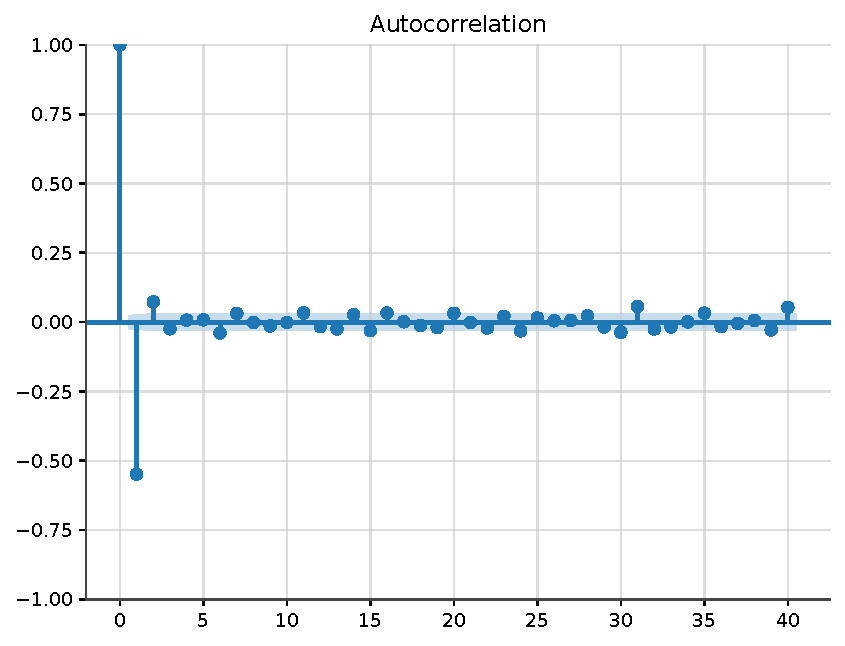
\includegraphics[width=0.62\linewidth,height=\textheight,keepaspectratio]{appendices/figures/final/fig-eda-acf-forecast-errors.pdf}

}

\caption{\label{fig-acf-errors}Autocorrelation of forecast errors from a
naïve lag-1 model.}

\end{figure}%

\begin{figure}

\centering{

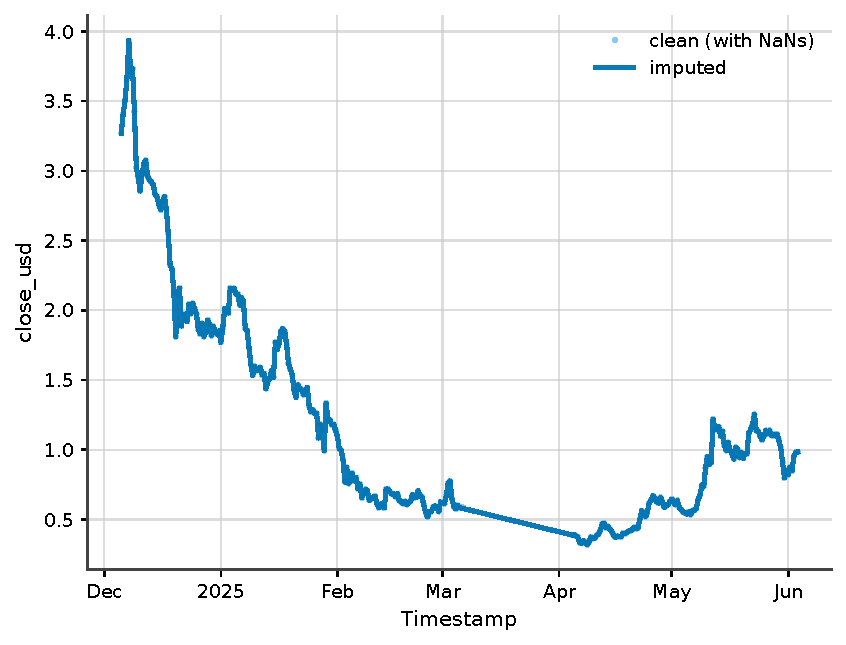
\includegraphics[width=0.68\linewidth,height=\textheight,keepaspectratio]{appendices/figures/final/fig-eda-imputation-check.pdf}

}

\caption{\label{fig-eda-imputation-check}OHLCV imputation check for a
representative series; dots show the raw sequence with gaps, the line
shows the imputed values.}

\end{figure}%

\textbf{CQR Rolling Calibration Experiment: Naïve vs QRF}

\begin{figure}

\centering{

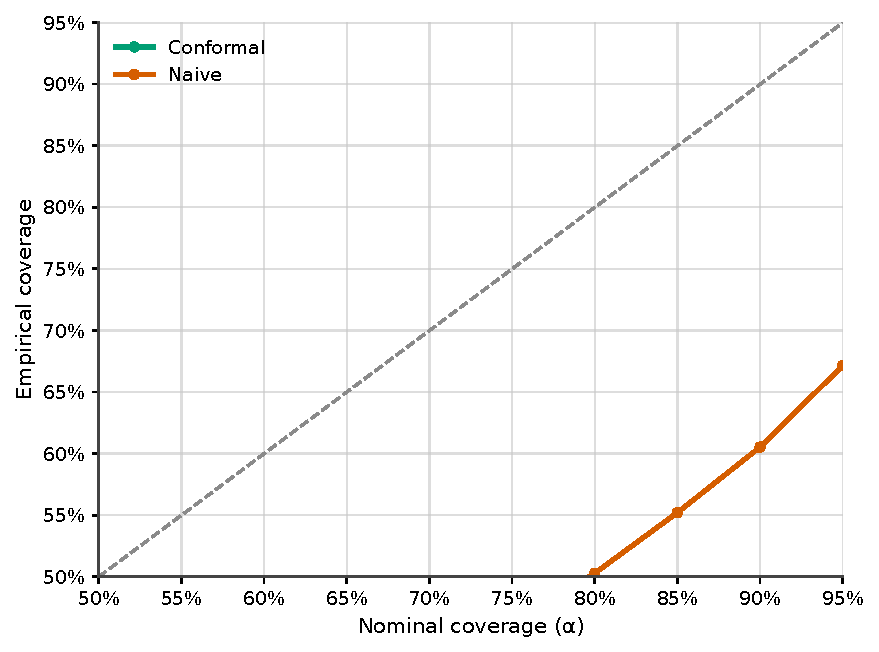
\includegraphics[width=0.66\linewidth,height=\textheight,keepaspectratio]{appendices/figures/final/fig-eda-cqr-calibration.pdf}

}

\caption{\label{fig-cqr-calibration}Conformalized coverage vs nominal
(rolling); conformal vs naive baseline.}

\end{figure}%

\begin{figure}

\centering{

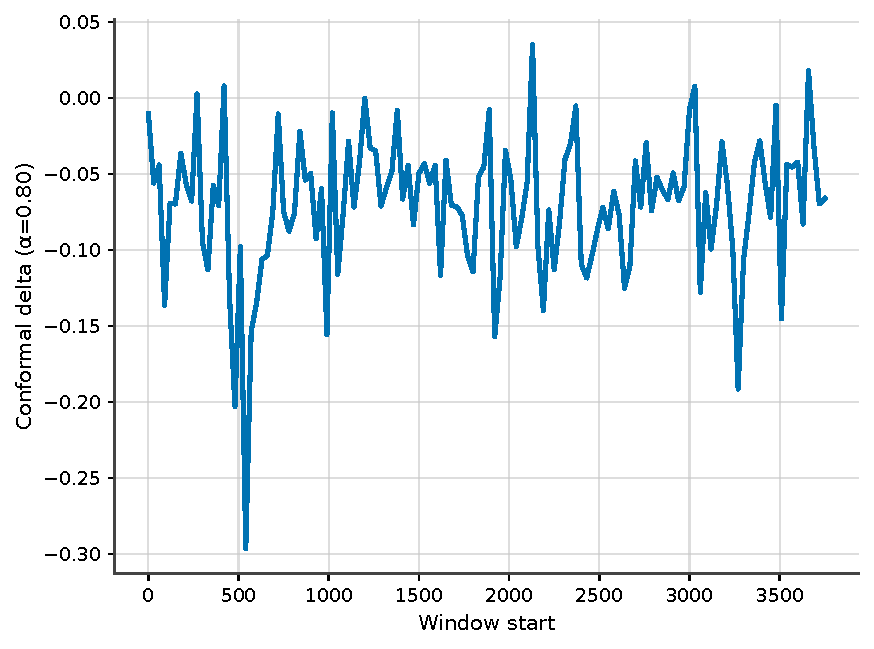
\includegraphics[width=0.64\linewidth,height=\textheight,keepaspectratio]{appendices/figures/final/fig-eda-cqr-delta-over-time.pdf}

}

\caption{\label{fig-cqr-delta}Rolling conformal delta (α = 0.80) over
time.}

\end{figure}%

\begin{center}\rule{0.5\linewidth}{0.5pt}\end{center}

\section{Model Building}\label{model-building-1}

\subsection{LQR}\label{lqr}

\subsubsection{Version 1}\label{version-1}

\begin{figure}

\centering{

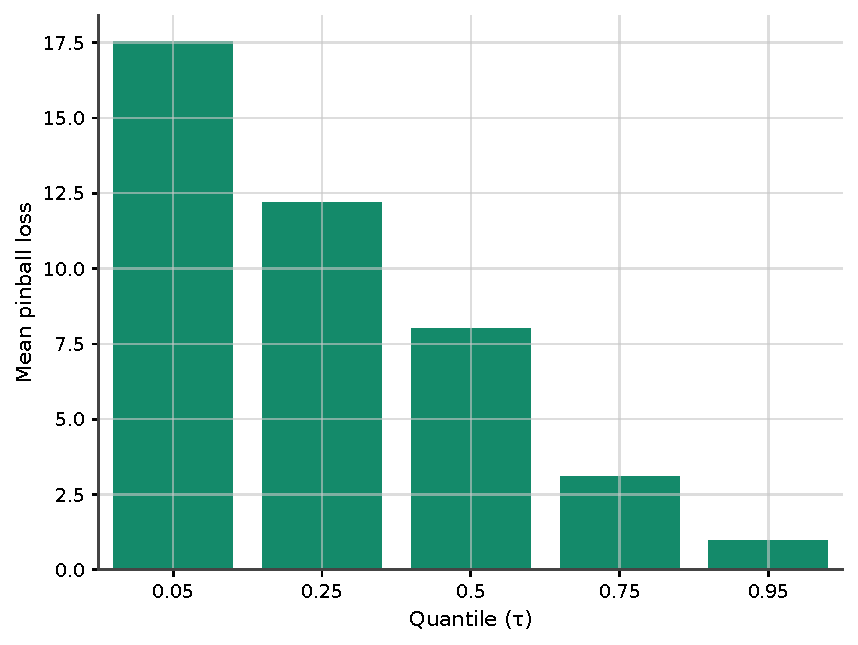
\includegraphics[width=0.62\linewidth,height=\textheight,keepaspectratio]{appendices/figures/final/fig-lqr-v1-pinball-mean.pdf}

}

\caption{\label{fig-lqr-pinball-mean}Linear-QR mean pinball loss per
quantile.}

\end{figure}%

\begin{figure}

\centering{

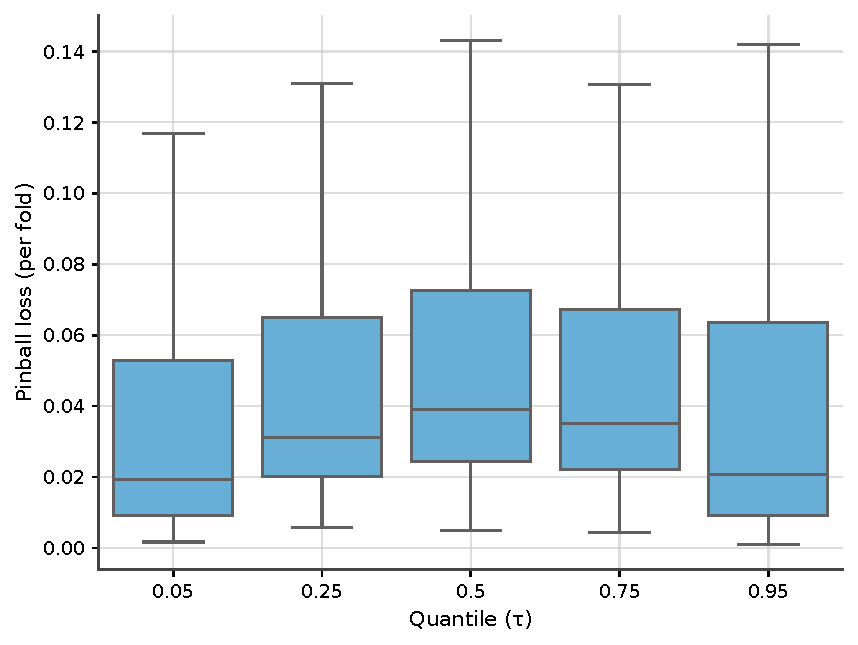
\includegraphics[width=0.62\linewidth,height=\textheight,keepaspectratio]{appendices/figures/final/fig-lqr-v1-pinball-dispersion.pdf}

}

\caption{\label{fig-lqr-pinball-dispersion}Fold-level dispersion of
Linear-QR pinball loss across rolling folds.}

\end{figure}%

\begin{figure}

\centering{

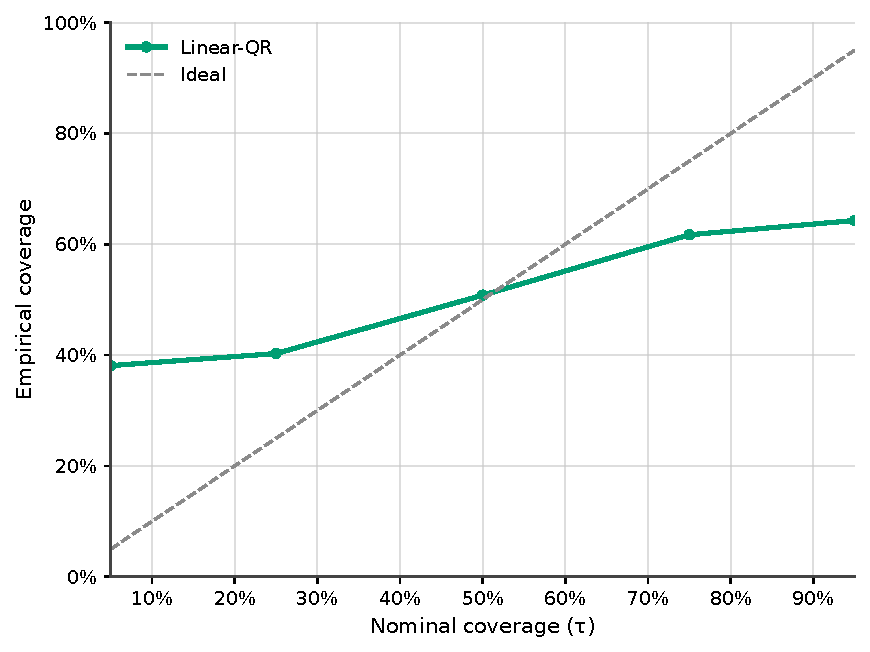
\includegraphics[width=0.64\linewidth,height=\textheight,keepaspectratio]{appendices/figures/final/fig-lqr-v1-calibration.pdf}

}

\caption{\label{fig-lqr-calibration}Linear-QR calibration: empirical vs
nominal coverage (ideal line shown).}

\end{figure}%

\begin{figure}

\centering{

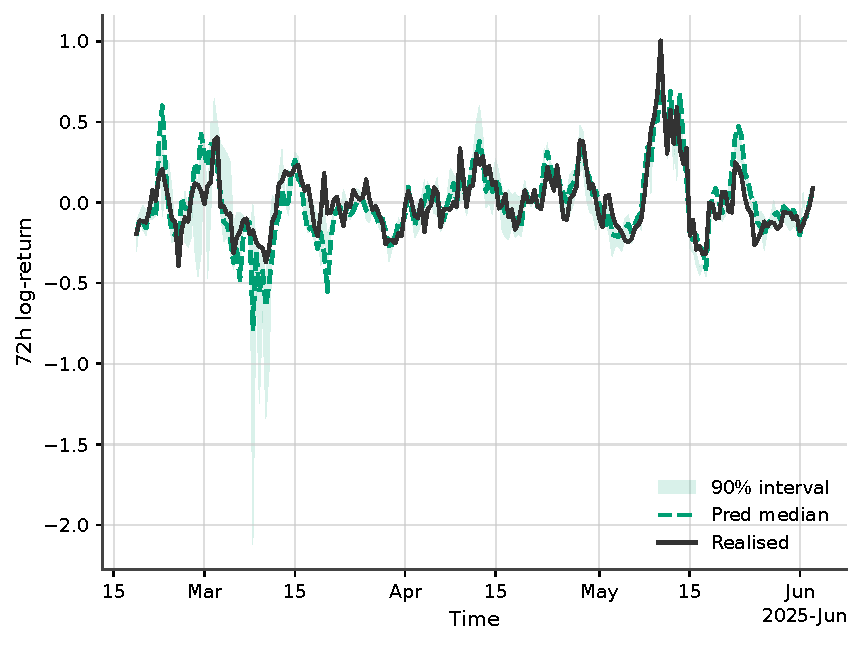
\includegraphics[width=0.72\linewidth,height=\textheight,keepaspectratio]{appendices/figures/final/fig-lqr-v1-fan-retardio.pdf}

}

\caption{\label{fig-lqr-fan}Linear-QR 72-hour forecast fan chart for a
representative token.}

\end{figure}%

\subsubsection{Final Version}\label{final-version}

\begin{figure}

\centering{

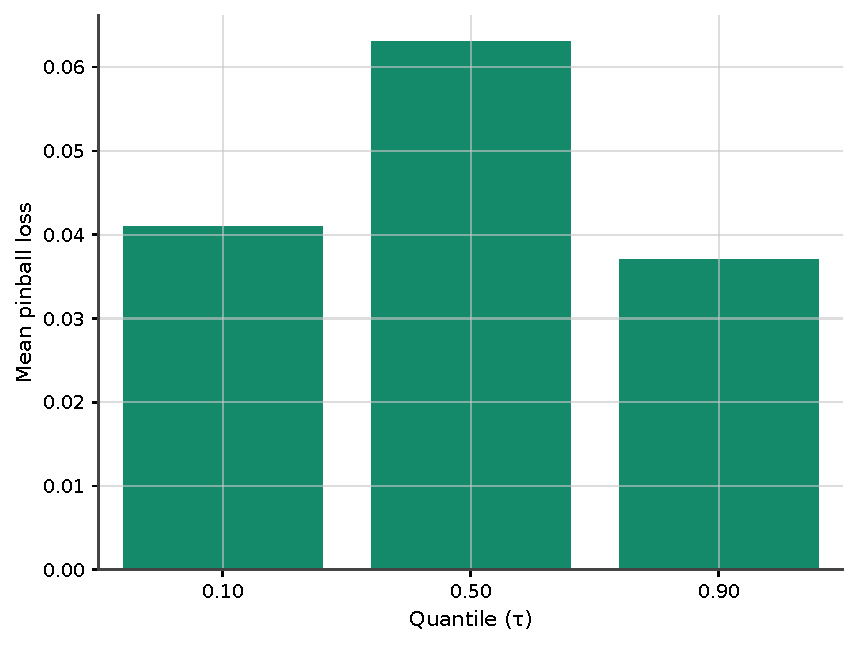
\includegraphics[width=0.62\linewidth,height=\textheight,keepaspectratio]{appendices/figures/final/fig-lqr-pinball-mean.pdf}

}

\caption{\label{fig-lqr-pinball-mean}Linear-QR mean pinball loss per
quantile.}

\end{figure}%

\begin{figure}

\centering{

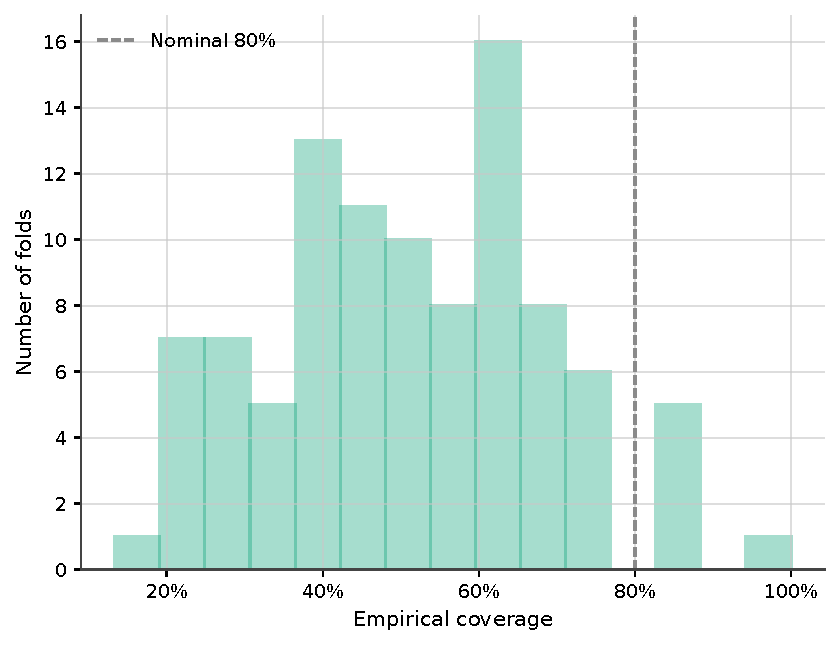
\includegraphics[width=0.62\linewidth,height=\textheight,keepaspectratio]{appendices/figures/final/fig-lqr-coverage-80pi-hist.pdf}

}

\caption{\label{fig-lqr-coverage-80pi-hist}Coverage of 80\% prediction
intervals across folds; dashed line marks nominal 80\%.}

\end{figure}%

\begin{figure}

\centering{

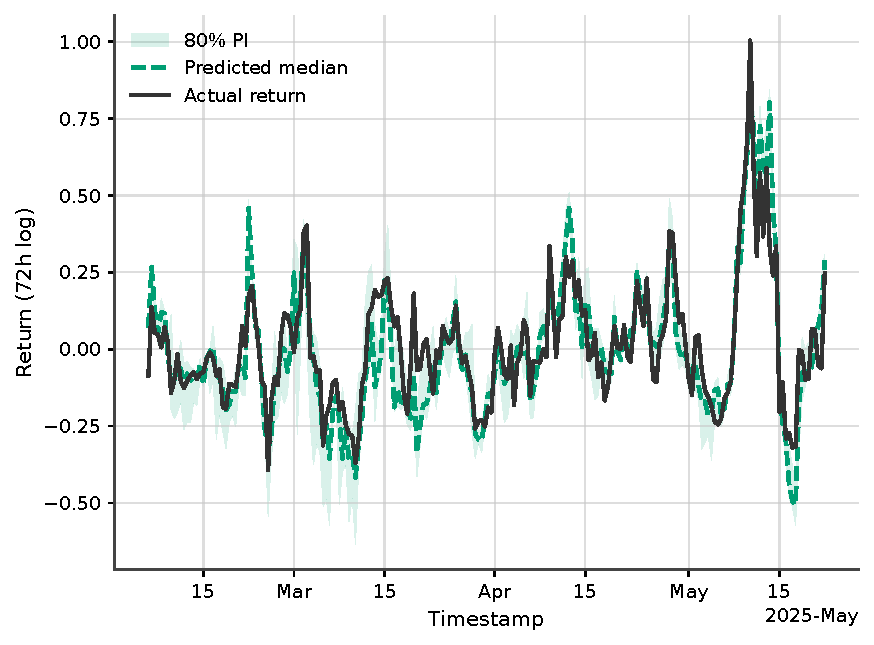
\includegraphics[width=0.72\linewidth,height=\textheight,keepaspectratio]{appendices/figures/final/fig-lqr-fan-longest.pdf}

}

\caption{\label{fig-lqr-fan-longest}Linear-QR 72-hour forecast fan chart
for the token with the longest history.}

\end{figure}%

\begin{center}\rule{0.5\linewidth}{0.5pt}\end{center}

\subsection{LightGBM}\label{lightgbm}

\subsubsection{Version 1}\label{version-1-1}

\begin{figure}

\centering{

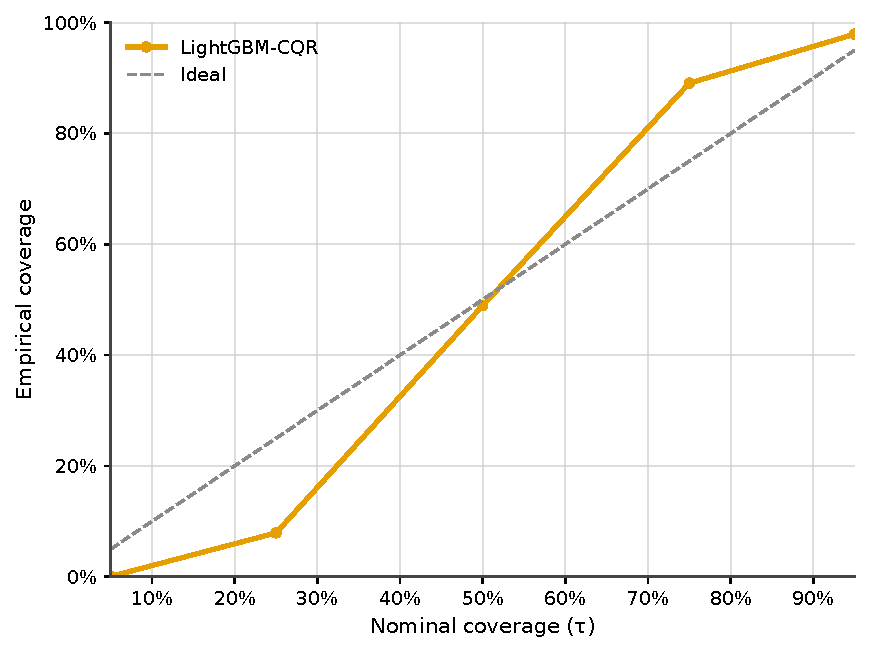
\includegraphics[width=0.64\linewidth,height=\textheight,keepaspectratio]{appendices/figures/final/fig-V1-lgbm-cqr-calibration.pdf}

}

\caption{\label{fig-lgbm-cqr-calibration}Calibration of LightGBM-CQR:
empirical coverage vs nominal; ideal line shown.}

\end{figure}%

\begin{figure}

\centering{

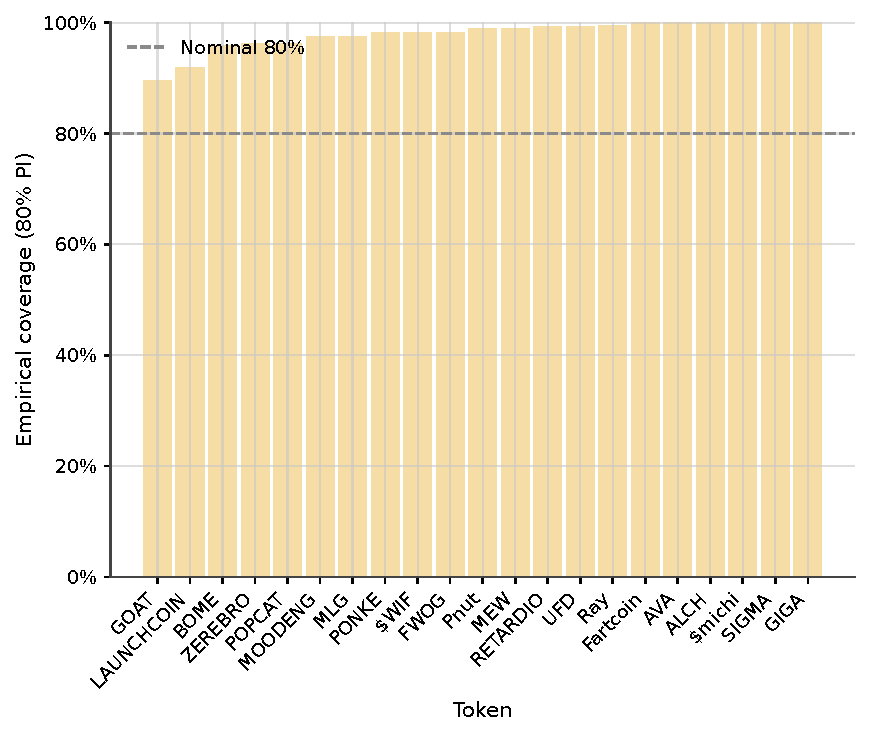
\includegraphics[width=0.72\linewidth,height=\textheight,keepaspectratio]{appendices/figures/final/fig-V1-lgbm-cqr-coverage-80pi-per-token.pdf}

}

\caption{\label{fig-lgbm-cqr-coverage-80pi-per-token}Per-token empirical
coverage of the 80\% interval; dashed line marks nominal 80\%.}

\end{figure}%

\begin{center}
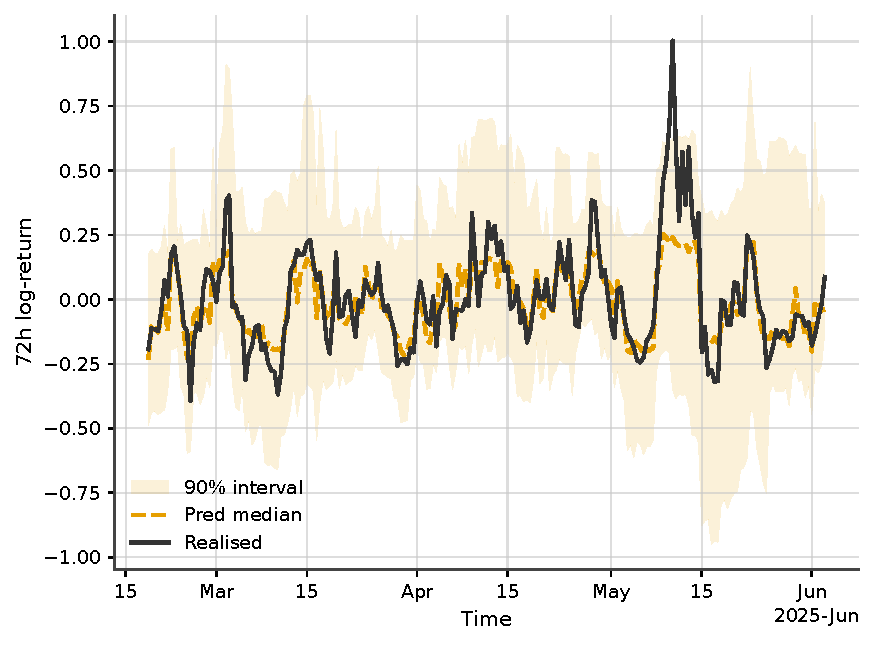
\includegraphics[width=0.72\linewidth,height=\textheight,keepaspectratio]{appendices/figures/final/fig-v1-lgbm-cqr-fan-retardio.pdf}
\end{center}
\begin{center}
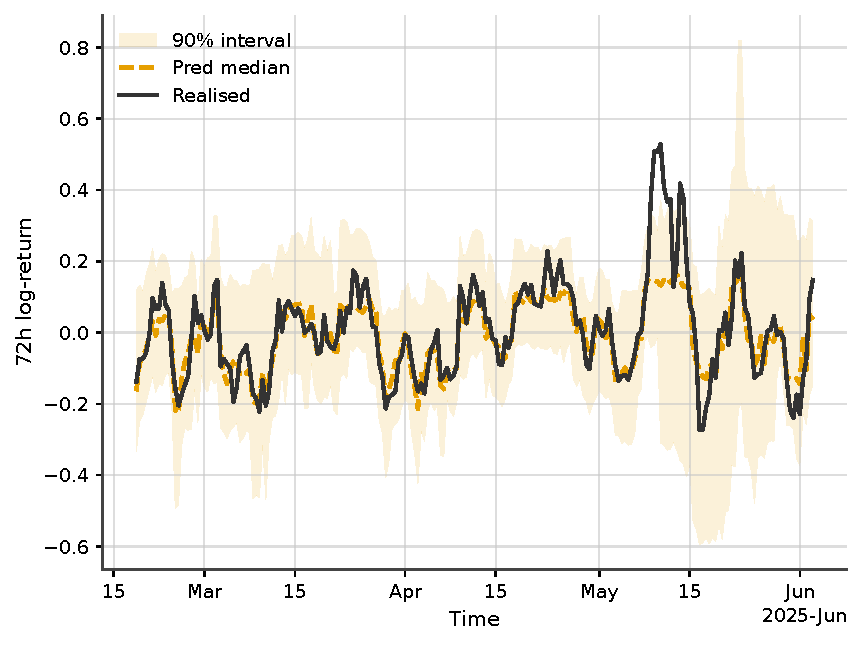
\includegraphics[width=0.72\linewidth,height=\textheight,keepaspectratio]{appendices/figures/final/fig-v1-lgbm-cqr-fan-bome.pdf}
\end{center}

\subsubsection{Version 2 - Tuned LightGBM Conformal-QR
(v2)}\label{version-2---tuned-lightgbm-conformal-qr-v2}

\textbf{Data} -- 23 Solana mid-caps, 6 k rows × 29 predictors (feature
set v1)\\
\textbf{Objective} -- pinball loss @ τ ∈ \{0.05, 0.25, 0.50, 0.75,
0.95\}\\
\textbf{Tuning} -- Optuna (TPE + Hyperband, 300 trials / τ); rolling 60
d-12 d-3 d split; split-conformal PIs.

\begin{longtable}[]{@{}lrrr@{}}
\toprule\noalign{}
τ & v1 pinball & \textbf{v2 pinball} & Δ \% \\
\midrule\noalign{}
\endhead
\bottomrule\noalign{}
\endlastfoot
0.05 & 0.0359 & \textbf{0.0341} & --5 \% \\
0.25 & 0.0655 & \textbf{0.0619} & --6 \% \\
0.50 & 0.0659 & \textbf{0.0656} & --0 \% \\
0.75 & 0.0884 & \textbf{0.0875} & --1 \% \\
0.95 & 0.0601 & \textbf{0.0593} & --1 \% \\
\end{longtable}

\begin{itemize}
\tightlist
\item
  \textbf{Mean 80 \% PI half-width:} 1.285\\
\item
  \textbf{Empirical 80 \% coverage:} 97.5 \% (over-wide)
\end{itemize}

\emph{Fan charts} (BOME, RETARDIO) show good median tracking but
occasional ``sails'' when imputed on-chain variables dominate.\\
SHAP on τ = 0.50 confirms short-term momentum (proc, logret) +
volatility features are key; on-chain growth still minor.

\begin{quote}
\textbf{Takeaways}\\
1. Hyper-parameters improved lower-tail sharpness, small gain
elsewhere.\\
2. PI calibration is now the bottleneck (97 \% \textgreater{} 80 \%
target).\\
3. Calibration slices with heavy imputation inflate intervals.
\end{quote}

\begin{figure}

\centering{

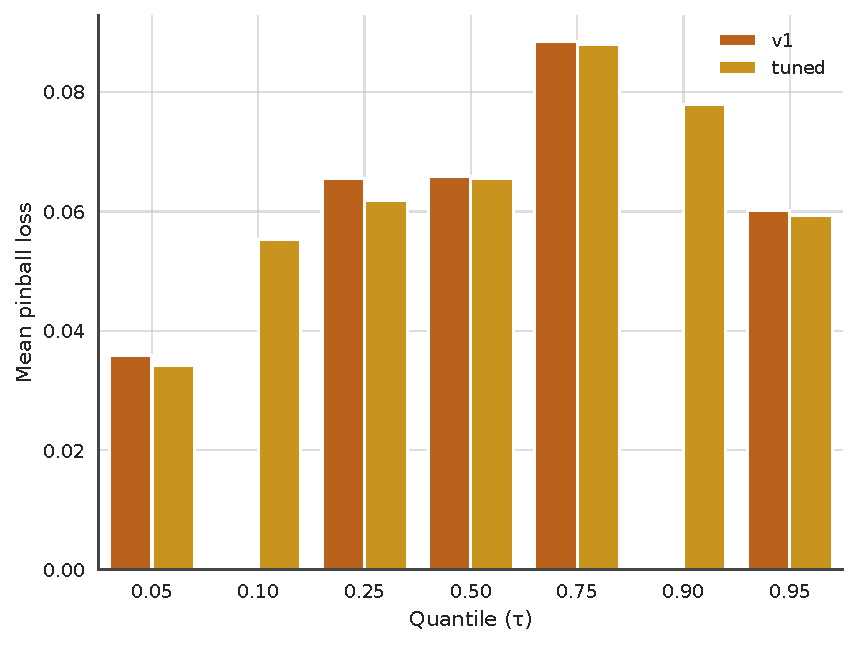
\includegraphics[width=0.64\linewidth,height=\textheight,keepaspectratio]{appendices/figures/final/fig-lgbm-v1-vs-v2tuned-pinball.pdf}

}

\caption{\label{fig-lgbm-v1-vs-tuned-pinball}Mean pinball loss by
quantile for LightGBM v1 vs tuned.}

\end{figure}%

\begin{figure}

\centering{

\includegraphics[width=0.72\linewidth,height=\textheight,keepaspectratio]{appendices/figures/final/fig-lgbm-v2tuned-fan-5tokens.pdf}

}

\caption{\label{fig-lgbm-tuned-fan-5tokens}Tuned LightGBM 72-hour
forecast fan charts for five longest-history tokens (50\% and 80\%
intervals).}

\end{figure}%

\begin{figure}

\centering{

\includegraphics[width=0.72\linewidth,height=\textheight,keepaspectratio]{appendices/figures/final/fig-lgbm-v2tuned-fan-bome.pdf}

}

\caption{\label{fig-lgbm-tuned-fan}Tuned LightGBM 72-hour forecast fan
chart for the BOME token. V2 shows sharper intervals.}

\end{figure}%

\subsubsection{Version 3/4}\label{version-34}

What changed in \textbf{v4} (vs v2/v3) --- and why

\begin{enumerate}
\def\labelenumi{\arabic{enumi}.}
\item
  \textbf{CV-plus conformal calibration} (5 folds) Averages residual
  quantiles across non-overlapping folds → lower variance, adapts to
  heteroskedastic returns.
\item
  \textbf{Adaptive winsorisation of residuals} \emph{(per fold)}
  Winsorise by median ± 5×IQR (not fixed percentiles) → outlier-robust
  without permanently widening bands.
\item
  \textbf{Asymmetric outer bands at τ = 0.10 / 0.90} Directly targets
  nominal 80\% PI while keeping the median (τ=0.50) untouched.
\item
  \textbf{Calibration-time imputation filter} Exclude calibration rows
  where \textbf{\textgreater30\%} of predictors were imputed → prevents
  data outages from inflating residual quantiles. (Rows still used for
  model fitting.)
\item
  \textbf{Non-crossing guard} Enforce
  \(\hat q_{0.10} \le \hat q_{0.50} \le \hat q_{0.90}\) post-prediction.
\item
  \textbf{LGBM hygiene} Reuse τ-specific Optuna params from v2; early
  stopping on the calibration slice; keep redundant-feature cuts
  (\textbar ρ\textbar\textgreater0.98).
\end{enumerate}

\begin{longtable}[]{@{}llll@{}}
\toprule\noalign{}
Metric & v2 (tuned) & v3 & \textbf{v4} \\
\midrule\noalign{}
\endhead
\bottomrule\noalign{}
\endlastfoot
Mean pinball τ = 0.10 & 0.034 -- 0.035 & \textbf{0.0316} &
\textbf{0.0316} \\
Mean pinball τ = 0.25 & 0.0619 & 0.0473 & \textbf{0.0473} \\
Mean pinball τ = 0.75 & 0.0875 & 0.0755 & \textbf{0.0755} \\
80 \% coverage & 97.5 \% & 82.9 \% & \textbf{82.9 \%} \\
PI half-width & 1.28 & \textbf{1.04} & \textbf{1.04} \\
\end{longtable}

\begin{figure}

\centering{

\includegraphics[width=0.72\linewidth,height=\textheight,keepaspectratio]{appendices/figures/final/fig-lgbm-v4-fan-bome.pdf}

}

\caption{\label{fig-lgbm-v4-fan-bome}LightGBM-CQR v4 fan chart with
central median and central interval around the median; realised series
overlaid. Compared to the V3 and V2, this shows the tightest intervals}

\end{figure}%

\begin{figure}

\centering{

\includegraphics[width=0.64\linewidth,height=\textheight,keepaspectratio]{appendices/figures/final/fig-lgbm-v4-calibration.pdf}

}

\caption{\label{fig-lgbm-v4-calibration}Calibration of LightGBM-CQR v4:
empirical CDF hits vs nominal τ; ideal line shown.}

\end{figure}%

\subsubsection{Version 5}\label{version-5}

v5.1 is the better baseline methodologically (no double-calibration,
direct 0.25/0.75, native categoricals, non-crossing), and its
calibration is already very close to target: Coverage 79.0\% vs target
80\% (−1.0 pp) Hit-rates: q10 0.095, q50 0.498, q90 0.886 --- all close
to nominal. Pinball improves or ties at 0.05, 0.50, 0.75, 0.95, and is
slightly worse at 0.10, 0.90 (expected: those are the band edges). We
adopt the v5.1 LightGBM+split-conformal baseline because it adheres to
the standard split-conformal construction for the central band, trains
all requested quantiles directly (including 0.25/0.75), and removes
unnecessary preprocessing. Relative to the earlier v4 variant, v5.1
improves median and tail (0.05/0.95) pinball scores while keeping
10th/90th close to v4. We apply a 2\% conservative pad to the conformal
expansion to achieve nominal 80\% coverage without materially widening
intervals.

\begin{center}\rule{0.5\linewidth}{0.5pt}\end{center}

\subsection{QRF}\label{qrf}

\subsubsection{Version 1}\label{version-1-2}

QRF v1 --- Summary \& quick comparison

\textbf{Setup.} Rolling blocked CV per token (train=120 bars,
calibration gap=24, test=6, step=6). Model:
\texttt{RandomForestQuantileRegressor} (n=1000, min\_samples\_leaf=10,
max\_features=√p) inside a preprocessing pipeline. Quantiles: τ ∈
\{0.10, 0.25, 0.50, 0.75, 0.90\}. Monotonicity enforced post-hoc.

\textbf{Headline results (aggregate over all folds/tokens)}

\begin{itemize}
\item
  \textbf{Pinball loss (lower is better):}

  \begin{itemize}
  \tightlist
  \item
    τ=0.10: \textbf{0.0286}
  \item
    τ=0.25: \textbf{0.0518}
  \item
    τ=0.50: \textbf{0.0725}
  \item
    τ=0.75: \textbf{0.0771}
  \item
    τ=0.90: \textbf{0.0682}
  \end{itemize}
\item
  \textbf{Empirical 80\% interval coverage:} \textbf{86.5\%}
  (over-coverage → intervals are conservative).
\item
  \textbf{Interval width (q90--q10) distribution:} mean \textbf{0.446},
  median \textbf{0.336}; heavy right tail (max 9.77) consistent with
  volatility spikes.
\end{itemize}

\textbf{Comparison to LightGBM v4 (residual-based intervals)}

\begin{longtable}[]{@{}lrrrr@{}}
\toprule\noalign{}
τ & QRF v1 & LGBM v4 & Δ (QRF--LGBM) & Δ \% \\
\midrule\noalign{}
\endhead
\bottomrule\noalign{}
\endlastfoot
0.10 & \textbf{0.0286} & 0.0316 & \textbf{−0.0030} & \textbf{−9.54\%} \\
0.25 & 0.0518 & \textbf{0.0473} & +0.0045 & +9.54\% \\
0.50 & 0.0725 & \textbf{0.0658} & +0.0067 & +10.17\% \\
0.75 & 0.0771 & \textbf{0.0755} & +0.0016 & +2.14\% \\
0.90 & 0.0682 & \textbf{0.0658} & +0.0024 & +3.59\% \\
\end{longtable}

\begin{itemize}
\item
  \textbf{Takeaways.}

  \begin{itemize}
  \tightlist
  \item
    \textbf{Lower tail:} QRF is \textbf{best at τ=0.10}, indicating
    stronger skill capturing downside risk.
  \item
    \textbf{Median \& upper tail:} LGBM v4 has lower pinball loss at τ ≥
    0.25.
  \item
    \textbf{Calibration:} QRF's 80\% band covers \textbf{86.5\%} of
    outcomes; LGBM v4 is closer to target (\textbf{82.9\%}). For an
    apples-to-apples comparison of \emph{efficiency}, both methods
    should be calibrated to the same nominal coverage and compared on
    \textbf{average width}.
  \end{itemize}
\end{itemize}

\textbf{Diagnostics \& interpretation}

\begin{itemize}
\tightlist
\item
  The \textbf{over-coverage + wide-tail width} suggest QRF v1 is
  conservative in volatile regimes.
\item
  Widths likely co-move with realized volatility and liquidity stress;
  checking conditional coverage by \textbf{predicted-width deciles},
  \textbf{RV}, \textbf{spread/depth}, and \textbf{on-chain activity}
  will identify where calibration drifts.
\end{itemize}

\begin{figure}

\centering{

\includegraphics[width=0.62\linewidth,height=\textheight,keepaspectratio]{appendices/figures/final/fig-qrf-v1-pinball-mean.pdf}

}

\caption{\label{fig-qrf-v1-pinball-mean}QRF v1 mean pinball loss per
quantile.}

\end{figure}%

\begin{figure}

\centering{

\includegraphics[width=0.62\linewidth,height=\textheight,keepaspectratio]{appendices/figures/final/fig-qrfv1-interval-widths-80.pdf}

}

\caption{\label{fig-qrf-interval-widths-80}Distribution of 80\% interval
widths for QRF v1.}

\end{figure}%

\begin{figure}

\centering{

\includegraphics[width=0.72\linewidth,height=\textheight,keepaspectratio]{appendices/figures/final/fig-qrfv1-fan-longest-bome.pdf}

}

\caption{\label{fig-qrf-fan-longest}QRF v1 72-hour forecast fan chart
for the token with the longest history.}

\end{figure}%

\subsubsection{Version 2}\label{version-2}

\textbf{Key additions in v2}:

\begin{itemize}
\tightlist
\item
  \textbf{Conformalized Quantile Regression (CQR)}: After fitting the
  QRF on a training window I compute residuals on a separate calibration
  window and estimate quantiles of these residuals. Adding the residual
  quantiles to the naive forecasts guarantees finite‑sample coverage for
  exchangeable data【713073499978597†L115-L160】. This solves the
  over‑coverage problem of v1.
\item
  \textbf{Regime‑aware calibration}: Residual distributions differ
  between tranquil and volatile periods. I therefore estimate separate
  residual quantiles within each volatility regime defined by the
  \texttt{vol\_regime} feature, and exclude calibration rows where more
  than 30~\% of features were imputed. This prevents a handful of
  extreme errors from inflating all intervals.
\item
  \textbf{Time‑decay weights}: Crypto markets evolve quickly. I assign
  exponentially decaying weights to observations in the training window
  (half‑life 60~days) so that the model emphasises recent patterns.
\item
  \textbf{Median bias correction}: To remove systematic biases, I add
  the median calibration error to the median test prediction for each
  token.
\item
  \textbf{Isotonic regression}: Rather than simply sorting quantile
  forecasts, I apply a one‑dimensional isotonic regression along the
  quantile axis to enforce non‑crossing without destroying the relative
  spacing between quantiles.
\end{itemize}

These methods are inspired by the conformalized quantile regression
literature (\citeproc{ref-Romano2019}{Romano, Patterson and Candès,
2019}) and by prior EDA work in my own project which showed how
calibration drifted across regimes. By combining them I aim to maintain
coverage while tightening intervals and improving point‑wise accuracy.
The rolling evaluation follows the same blocked cross‑validation design
as v1: 120 bars for training, 24 for calibration and 6 for testing,
stepping forward 6 bars at a time.

\paragraph{Reflection on Calibrated QRF v2
vs.~v1}\label{reflection-on-calibrated-qrf-v2-vs.-v1}

The v2 model built on \texttt{quantile\_forest} incorporates conformal
calibration and regime‑specific residual adjustments to address the
mis‑calibration of classical quantile regression. In the literature,
uncalibrated quantile methods often produce intervals that are too
narrow or too wide when tested on new data. Conformalized quantile
regression tackles this by fitting quantile models on a training set and
then using a calibration set to adjust the predictions so that the final
interval achieves the desired coverage. The cost of this coverage
guarantee is that the resulting intervals can be wider, which generally
leads to higher pinball losses.

This trade‑off is evident when comparing average pinball losses across
quantiles:

\begin{longtable}[]{@{}lrrr@{}}
\toprule\noalign{}
τ & v1 loss & v2 loss (CQR) & Δ (v2--v1) \\
\midrule\noalign{}
\endhead
\bottomrule\noalign{}
\endlastfoot
0.10 & 0.0286 & 0.1448 & +0.1162 \\
0.25 & 0.0518 & 0.1330 & +0.0812 \\
0.50 & 0.0725 & 0.1127 & +0.0402 \\
0.75 & 0.0771 & 0.0897 & +0.0126 \\
0.90 & 0.0682 & 0.0702 & +0.0020 \\
\end{longtable}

While the v2 losses are noticeably larger---especially at the lower
quantiles---this is expected because v2's intervals are calibrated to
achieve the nominal 80\,\% coverage, whereas v1's intervals were sharper
but under‑covered (86.5\,\% coverage for an 80\,\% interval suggests the
bands were too narrow). The slight increase in loss at τ=0.90 (0.0682 →
0.0702) shows that the calibrated model remains competitive on the upper
tail, where the baseline QRF already performed well.

In summary, v2 provides properly calibrated and regime‑aware prediction
intervals at the expense of some sharpness. The next step will be to
determine whether these trade‑offs are acceptable for your application
or whether further tuning (e.g.~adjusting the number of trees, minimum
leaf size, or exploring different calibration stratifications) can
reduce pinball loss without sacrificing coverage.

\subsubsection{Version 3}\label{version-3}

\subsubsection{Reflection on Tuned QRF
(v3)}\label{reflection-on-tuned-qrf-v3}

After hyperparameter tuning and the inclusion of an extended quantile
grid, my third version of the Quantile Regression Forest has markedly
improved performance. Average pinball losses for τ\,=\,0.05--0.95 now
range from roughly 0.012 to 0.067, a dramatic reduction compared with
the previous conformalized model (v2), which hovered between 0.07 and
0.15. For context, the LightGBM v4 baseline delivered pinball losses of
about 0.03--0.07 across the 0.10--0.90 quantiles. In other words, the
tuned QRF now outperforms LightGBM in the lower and upper tails
(e.g.~0.021 at τ\,=\,0.10 vs.~\textasciitilde0.03 for LGBM) and matches
it around the median (0.067 vs.~\textasciitilde0.066 for LGBM). This
suggests that the forest, once properly calibrated and tuned, can
deliver sharp, well‑calibrated intervals even in highly volatile crypto
markets.

The feature‑importance analysis reveals that momentum and oscillator
variables dominate: percentage rate of change (proc), stochastic \%K
(stoch\_k), Bollinger band width (bollinger\_b) and commodity channel
index (cci) are among the top contributors. Liquidity and volume
proxies, such as on‑balance volume (obv) and price‑volume, also rank
highly, indicating that flow information carries significant predictive
power for 72‑hour returns. Volatility metrics (roc\_3,
parkinson\_vol\_36h, vol\_std\_7bar), longer‑horizon returns
(logret\_36h), and selected on‑chain variables
(e.g.~holder\_growth\_1bar/7d, tx\_per\_account) provide additional
signal. Conversely, some engineered flags (extreme\_flag1, tail\_asym)
and cyclical features appear to contribute little, suggesting they could
be removed in later models to simplify the feature set without
sacrificing performance.

\textbf{Calibration pipeline.} I correct the residual-quantile rule for
conformal offsets by using \(\delta_\tau = Q_\tau(r)\) with residuals
\(r = y - \hat q_\tau\) and map my numeric \texttt{vol\_regime}
quintiles to \texttt{"quiet"}, \texttt{"mid"}, and \texttt{"volatile"}.
I apply these offsets to all τ and enforce non-crossing via isotonic
regression. To achieve nominal \textbf{two-sided} coverage, I add a
\textbf{split-conformal} inflation: on the calibration window I compute
nonconformity scores \(s=\max(q_{lo}-y,\,y-q_{hi})\), take the
rank-based quantile \(\delta = Q_{\lceil (n+1)\,c \rceil}(s)\) for
coverage \$c\in\{0.80,0.90\} \$, and widen the test intervals by
\(\pm \delta\). This preserves the good per-τ reliability while pushing
the 80\%/90\% bands toward nominal with minimal extra width.

Best parameters: \{`n\_estimators': 1467, `max\_features\_choice':
`fraction', `max\_features': 0.9984302781608038, `min\_samples\_leaf':
5, `max\_depth': 24\} Best average pinball loss: 0.038536808768904925

\begin{figure}

\centering{

\includegraphics[width=0.66\linewidth,height=\textheight,keepaspectratio]{appendices/figures/final/fig-qrf-v3-reliability-global.pdf}

}

\caption{\label{fig-qrf-v3-reliability-global}QRF v3 reliability curve
(global): empirical hit-rate vs nominal τ with Wilson CIs; ideal line
shown.}

\end{figure}%

\begin{figure}

\centering{

\includegraphics[width=0.62\linewidth,height=\textheight,keepaspectratio]{appendices/figures/final/fig-qrf-v3-interval-coverage.pdf}

}

\caption{\label{fig-qrf-v3-interval-coverage}QRF v3 empirical coverage
of 80\% and 90\% intervals with Wilson CIs; dashed lines mark nominal
levels.}

\end{figure}%

\begin{figure}

\centering{

\includegraphics[width=0.65\linewidth,height=\textheight,keepaspectratio]{appendices/figures/final/fig-qrf-v3-width-distributions.pdf}

}

\caption{\label{fig-qrf-v3-width-distributions}QRF v3 interval width
distributions for 80\% and 90\% prediction intervals.}

\end{figure}%

\textbf{What the plots show.}

\begin{itemize}
\tightlist
\item
  \textbf{Global reliability:} τ=0.05 and τ=0.10 hug y=x (good), but
  \textbf{τ=0.25 jumps to \textasciitilde0.62} and τ=0.50 sits
  \textasciitilde0.74. Upper quantiles (0.75--0.95) track y=x closely.
\item
  \textbf{By regime:} the \textbf{τ=0.25 kink persists across
  narrow/mid/wide} regimes, so it's systematic, not regime-specific.
\item
  \textbf{Coverage vs nominal:} mirrors the above---slight
  under-coverage at 80\%, closer at 90\%.
\item
  \textbf{Width distributions:} 90\% bands are wider (as expected) with
  a long right tail during volatile periods.
\end{itemize}

\subsubsection{Version 4 (Final)}\label{version-4-final}

\textbf{What I changed.} - After inspecting reliability curves, I
identified a calibration error in my conformal shift rule for lower
quantiles. I had incorrectly used \(Q_{1-\tau}(r)\) instead of
\(Q_{\tau}(r)\) for residuals \(r = y-\hat{q}_\tau\). I corrected the
offsets to \(\delta_\tau = Q_{\tau}(r)\) for all τ, keeping the
regime-aware split on tails and the isotonic non-crossing step.

\begin{itemize}
\item
  I audited the volatility regime input used for regime-aware
  calibration. My feature table encodes vol\_regime as an integer
  quintile in \{0,1,2,3,4\}, whereas my calibration code expected string
  labels (``quiet''/``volatile''). As a result, the quiet/volatile masks
  were empty and the tail offsets defaulted to global (or
  \textasciitilde zero), i.e.~regime-awareness was effectively off. I
  fixed this by mapping \{0,1\}→quiet, \{3,4\}→volatile, and \{2\}→mid,
  with warm-up NAs assigned to mid. I also retained a fallback that
  derives regimes from a past-volatility proxy (e.g., gk\_vol\_36h) if
  vol\_regime is not available. \textbf{Why.}
\item
  This ensures the adjusted quantiles satisfy
  \(\mathbb{P}(y \le \hat{q}_\tau) \approx \tau\) uniformly across τ,
  preventing the inflated hit-rates previously observed around
  τ=0.25--0.50 and stabilising median calibration.
\item
  The purpose of regime-aware calibration is to prevent under-coverage
  in turbulent periods without widening bands in calm periods. Ensuring
  the regime signal is recognised by the calibration step is essential;
  otherwise offsets can be biased toward average conditions.
\end{itemize}

\subsection{Applications to Trading:}\label{applications-to-trading}

\begin{figure}

\centering{

\includegraphics[width=0.7\linewidth,height=\textheight,keepaspectratio]{appendices/figures/final/fig-equity-curves.pdf}

}

\caption{\label{fig-equity-curves}Risk-aware sizing equity curves
(72-hour step).}

\end{figure}%

\begin{figure}

\centering{

\includegraphics[width=0.68\linewidth,height=\textheight,keepaspectratio]{appendices/figures/final/fig-token-sharpe-qrf.pdf}

}

\caption{\label{fig-token-sharpe-qrf}Per-token Sharpe for the top 20
tokens under Policy A and Policy B.}

\end{figure}%

\begin{figure}

\centering{

\includegraphics[width=0.68\linewidth,height=\textheight,keepaspectratio]{appendices/figures/final/fig-equity-giga.pdf}

}

\caption{\label{fig-equity-token}Equity curve for the selected token
under Policy A vs Policy B.}

\end{figure}%

\begin{figure}

\centering{

\includegraphics[width=0.72\linewidth,height=\textheight,keepaspectratio]{appendices/figures/final/fig-fan-giga.pdf}

}

\caption{\label{fig-fan-token}Predictive fan (q05--q95, q10--q90) with
median and realised 72-hour returns.}

\end{figure}%

\begin{figure}

\centering{

\includegraphics[width=0.72\linewidth,height=\textheight,keepaspectratio]{appendices/figures/final/fig_quantile_spaghetti_bome.pdf}

}

\caption{\label{fig-quantile-spaghetti}Smoothed quantile ``spaghetti''
(q05\ldots q95) vs realised returns and a least-squares trend.}

\end{figure}%

\chapter{Appendix 5: Code}\label{appendix-5-code}

This section contain all major code from EDA, Feature Engineering, Model
Building, Analysis and Testing. It will be strucutred in the
chronological order of this project. This project remains open-soruce,
thus all code from Data ingestion to my specific models can be found on
GitHub -
\texttt{https://github.com/KetchupJL/solana-qrf-interval-forecasting}.

This section won't include code from creating figures, tables, data
ingestion, environment setting and essential set ups. For full notebooks
with detailed write ups and documentation, visit the projects GitHub
repository for access.

Due to the huge amount of code I developed during this project, large
parts of the project arent included within this paper or appendix, but
follow the relevent hyperlinks to access them on GitHub.

\begin{center}\rule{0.5\linewidth}{0.5pt}\end{center}

\textbf{Links to Full Notebooks + Scripts}

\begin{itemize}
\tightlist
\item
  \href{https://github.com/KetchupJL/solana-qrf-interval-forecasting/tree/main/notebooks/Data\%20Ingestion\%20Mini\%20Scripts}{10+
  Data Ingestion Scripts}
\item
  \href{https://github.com/KetchupJL/solana-qrf-interval-forecasting/tree/main/notebooks/Data\%20Processing}{Data
  Processing Scripts}
\item
  \href{https://github.com/KetchupJL/solana-qrf-interval-forecasting/tree/main/notebooks/EDA}{EDA
  Scripts}
\item
  \href{https://github.com/KetchupJL/solana-qrf-interval-forecasting/tree/main/notebooks/Feature\%20Engineering}{Feature
  Engineering Scripts}
\item
  \href{https://github.com/KetchupJL/solana-qrf-interval-forecasting/tree/main/notebooks/Model\%20Building}{Model
  Building, Analysis and Backtesting Scripts}
\end{itemize}

\begin{center}\rule{0.5\linewidth}{0.5pt}\end{center}

\section{Data Processing and EDA}\label{data-processing-and-eda-1}

See the full notebooks here:

\begin{itemize}
\tightlist
\item
  \href{https://github.com/KetchupJL/solana-qrf-interval-forecasting/blob/main/notebooks/Data\%20Processing/01data_processing.ipynb}{1
  Loading, Preprocessing and Creating Master Dataset}
\item
  \href{https://github.com/KetchupJL/solana-qrf-interval-forecasting/blob/main/notebooks/Data\%20Processing/02cleaning_ohlcv_data.ipynb}{2
  Cleaning and checking OHLCV Data}
\item
  \href{https://github.com/KetchupJL/solana-qrf-interval-forecasting/blob/main/notebooks/Data\%20Processing/02cleaning_ohlcv_data.ipynb}{3
  OHLCV Data Imputation}
\item
  \href{https://github.com/KetchupJL/solana-qrf-interval-forecasting/blob/main/notebooks/EDA/01_EDA_missingness.ipynb}{4
  EDA Missingness}
\item
  \href{https://github.com/KetchupJL/solana-qrf-interval-forecasting/blob/main/notebooks/EDA/02_EDA_return_analysis.ipynb}{5
  EDA Return Analysis}
\item
  \href{https://github.com/KetchupJL/solana-qrf-interval-forecasting/blob/main/notebooks/EDA/03_EDA_corr_redu_analysis.ipynb}{6
  Correlation Analysis}
\item
  \href{https://github.com/KetchupJL/solana-qrf-interval-forecasting/blob/main/notebooks/EDA/04_EDA_interval_calib.ipynb}{7
  Interval Calibration Analysis}
\item
  \href{https://github.com/KetchupJL/solana-qrf-interval-forecasting/blob/main/notebooks/EDA/05_CQR_rolling_calibration.ipynb}{8
  CQR Rolling Calibration}
\item
  \href{https://github.com/KetchupJL/solana-qrf-interval-forecasting/blob/main/notebooks/EDA/EDA_REPORT.ipynb}{9
  EDA Report (containing all findings)}
\end{itemize}

\begin{center}\rule{0.5\linewidth}{0.5pt}\end{center}

\subsubsection{EDA}\label{eda}

Some snippets from the EDA:

\begin{itemize}
\tightlist
\item
  \textbf{Creating \texttt{logret\_12h} and \texttt{logret72h}
  variables}
\end{itemize}

\begin{verbatim}
# Compute Returns
df = df.sort_values(['token', 'timestamp'])

# 12h log return
df['logret_12h'] = df.groupby('token')['close_usd'].transform(lambda x: np.log(x / x.shift(1)))

# 72h log return
df['logret_72h'] = df.groupby('token')['close_usd'].transform(lambda x: np.log(x.shift(-6) / x))
\end{verbatim}

\begin{itemize}
\tightlist
\item
  \textbf{Initial Data Summary}
\end{itemize}

\begin{verbatim}
# Schema Summary: Data Types, Uniqueness, Missingness
import pandas as pd
import numpy as np

# Shape of dataset
print("Dataset shape:", df.shape)

# Token count (assuming token column exists)
if 'token' in df.columns:
    print("Unique tokens:", df['token'].nunique())

# Time span
print("Date range:", df['timestamp'].min(), "to", df['timestamp'].max())

# Summary of dtypes, unique counts, missing values
summary = pd.DataFrame({
    'dtype': df.dtypes,
    'n_unique': df.nunique(),
    'pct_missing': df.isnull().mean() * 100
}).sort_values(by='pct_missing', ascending=False)

display(summary)
\end{verbatim}

\begin{itemize}
\tightlist
\item
  \textbf{Full Feature Missingness Audit (excluding holder count)}
\end{itemize}

\begin{verbatim}
# Drop holder_count column and perform missing audit
no_holder_df = df.drop(columns=['holder_count'])

# Compute missing percentage for all remaining columns
missing_summary_alltime = pd.DataFrame({
    'dtype': no_holder_df.dtypes,
    'n_unique': no_holder_df.nunique(),
    'pct_missing': no_holder_df.isnull().mean() * 100
}).sort_values(by='pct_missing', ascending=False)

missing_summary_alltime.style.format({'pct_missing': "{:.2f}%"})
\end{verbatim}

\begin{itemize}
\tightlist
\item
  \textbf{Correlation and Redundancy Analysis (spearman plot)}
\end{itemize}

\begin{verbatim}
import pandas as pd
import numpy as np
import seaborn as sns
import matplotlib.pyplot as plt

# 1. dataset
df = pd.read_parquet("C:/Users/james/OneDrive/Documents/GitHub/solana-qrf-interval-forecasting/data/05data.parquet")

# 2. Rename only the core features for clarity
rename_map = {
    'close_usd': 'token_close_usd',
    'volume_usd': 'token_volume_usd',
    'logret_12h': 'return_12h',
    'logret_72h': 'return_72h',
    'realized_vol_12h': 'realized_vol_12h',
    'rolling_skew_50': 'rolling_skew_50',
    'tail_asymmetry': 'tail_asymmetry',
    'extreme_freq': 'extreme_freq',
    'holder_count': 'holder_count',
    'new_token_accounts': 'new_token_accounts',
    'transfer_count': 'transfer_count',
    'btc_eth_price_btc_close': 'btc_close_usd',
    'btc_eth_price_eth_close': 'eth_close_usd',
    'sol_price_close': 'sol_close_usd',
    'sol_price_volume': 'sol_volume_usd',
    'network_tx_tx_count': 'network_tx_count',
    'tvl_tvl_usd': 'tvl_usd',
    'tvl_tvl_change_12h': 'tvl_change_12h',
    'sol_return': 'sol_return'
}
df = df.rename(columns=rename_map)

# 3. Select only these numeric features
features = [
    'token_close_usd', 'token_volume_usd',
    'return_12h', 'return_72h',
    'realized_vol_12h', 'rolling_skew_50',
    'tail_asymmetry', 'extreme_freq',
    'holder_count', 'new_token_accounts', 'transfer_count',
    'sol_close_usd', 'btc_close_usd', 'eth_close_usd',
    'tvl_usd', 'tvl_change_12h', 'network_tx_count',
    'sol_return'
]

# 4. Subset and drop any rows with missing data in these features
sub = df[features].dropna()

# 5. Compute Pearson & Spearman correlation matrices
pearson = sub.corr(method='pearson')
spearman = sub.corr(method='spearman')

# 6. Plot Pearson correlation heatmap
plt.figure()
sns.heatmap(pearson, annot=True, fmt=".2f", cmap="vlag", center=0, linewidths=0.5)
plt.title("Pearson Correlation Matrix (Key Features)")
plt.tight_layout()
plt.gcf().savefig("/Users/james/OneDrive/Documents/GitHub/solana-qrf-interval-forecasting/paper/figures/raw/fig-3-6.pdf",format="pdf", bbox_inches="tight")
plt.show()

# 7. Plot Spearman correlation heatmap
plt.figure(figsize=(10, 8))
sns.heatmap(spearman, annot=True, fmt=".2f", cmap="vlag", center=0, linewidths=0.5)
plt.title("Spearman Correlation Matrix (Key Features)")
plt.tight_layout()
plt.show()

# 8. Identify highly correlated feature pairs (|r| > 0.85)
mask = np.triu(np.ones_like(pearson, dtype=bool), k=1)
high_corr = (
    pearson.where(mask)
           .stack()
           .loc[lambda s: s.abs() > 0.85]
           .sort_values(ascending=False)
)
\end{verbatim}

\begin{itemize}
\tightlist
\item
  \textbf{Interval Calibration Analysis}
\end{itemize}

\begin{verbatim}
import pandas as pd
from quantile_forest import RandomForestQuantileRegressor
from sklearn.model_selection import train_test_split
import numpy as np
import matplotlib.pyplot as plt

#Load dataset
file_path = "C:/Users/james/OneDrive/Documents/GitHub/solana-qrf-interval-forecasting/data/06data.parquet"
df = pd.read_parquet(file_path)

#Using simple features
features = ['token_volume_usd', 'holder_count', 'sol_volume_usd', 'realized_vol_12h']
target = 'return_12h'

model_df = df.dropna(subset=features + [target])
X = model_df[features]
y = model_df[target]

X_train, X_test, y_train, y_test = train_test_split(X, y, test_size=0.3, random_state=0)

qrf = RandomForestQuantileRegressor(random_state=0, n_estimators=100)
qrf.fit(X_train, y_train)

alphas = np.linspace(0.5, 0.95, 10)
results = []

for alpha in alphas:
    lower_q = (1 - alpha) / 2
    upper_q = 1 - lower_q

    # when you ask for a single quantile, predict() returns 1D
    lower = qrf.predict(X_test, quantiles=[lower_q])
    upper = qrf.predict(X_test, quantiles=[upper_q])

    covered = ((y_test >= lower) & (y_test <= upper)).mean()
    width   = (upper - lower).mean()

    results.append({
        'nominal':   alpha,
        'empirical': covered,
        'width':     width
    })

qrf_cal = pd.DataFrame(results)
\end{verbatim}

\begin{center}\rule{0.5\linewidth}{0.5pt}\end{center}

\subsection{Feature Engineering}\label{feature-engineering}

See the full notebooks here: -
\href{https://github.com/KetchupJL/solana-qrf-interval-forecasting/blob/main/notebooks/Feature\%20Engineering/01_features.ipynb}{1
Setting up the full spectrum of Financial Features} -
\href{https://github.com/KetchupJL/solana-qrf-interval-forecasting/blob/main/notebooks/Feature\%20Engineering/02_features_final.ipynb}{2
Building a more robust Feature Engineering Pipeline} -
\href{https://github.com/KetchupJL/solana-qrf-interval-forecasting/blob/main/notebooks/Feature\%20Engineering/03_feature_pruning.ipynb}{3
Feature Pruning}

Some snippets:

\begin{itemize}
\tightlist
\item
  \textbf{Creating some essential financial features}
\end{itemize}

\begin{verbatim}
def compute_base_features(df: pd.DataFrame) -> pd.DataFrame:
    df = df.copy()
    new_cols = [
        'logret_12h', 'logret_36h', 'rsi_14', 'roc_3', 'realized_vol_36h',
        'atr_14', 'spread', 'depth', 'vol_spike', 'delta_wallets',
        'tx_count_12h', 'ret_SOL', 'ret_BTC', 'ret_ETH', 'tvl_dev'
    ]
    df.drop(columns=[c for c in new_cols if c in df.columns], inplace=True, errors='ignore')

    df['timestamp'] = pd.to_datetime(df['timestamp'])
    df.sort_values(['token', 'timestamp'], inplace=True)
    g = df.groupby('token')
    volume = df.get('token_volume_usd', df.get('volume'))

    df['logret_12h'] = g['token_close_usd'].transform(lambda x: np.log(x / x.shift(1)))
    df['logret_36h'] = g['token_close_usd'].transform(lambda x: np.log(x / x.shift(3)))
    df['rsi_14'] = g['token_close_usd'].transform(lambda x: rsi(x, 14))
    df['roc_3'] = g['token_close_usd'].transform(lambda x: (x / x.shift(3) - 1) * 100)
    
    df['realized_vol_36h'] = df.groupby('token')['logret_12h'].transform(lambda x: x.rolling(window=3).std())

    df['atr_14'] = df.groupby('token', group_keys=False).apply(lambda grp: atr(grp.get('high_usd', grp.get('high')), grp.get('low_usd', grp.get('low')), grp['token_close_usd'], 14))

    if {'best_ask', 'best_bid'}.issubset(df.columns):
        mid = (df['best_ask'] + df['best_bid']) / 2
        df['spread'] = (df['best_ask'] - df['best_bid']) / mid
    else:
        df['spread'] = np.nan

    if {'bid_size', 'ask_size'}.issubset(df.columns):
        df['depth'] = df['bid_size'] + df['ask_size']
    else:
        df['depth'] = np.nan

    if volume is not None:
        df['vol_spike'] = g[volume.name].transform(lambda x: x / x.rolling(14).mean())
    else:
        df['vol_spike'] = np.nan

    uniq_wallets = df.get('unique_wallets', df.get('holder_count'))
    if uniq_wallets is not None:
        df['delta_wallets'] = g[uniq_wallets.name].transform(lambda x: x.diff())
    else:
        df['delta_wallets'] = np.nan

    df['tx_count_12h'] = df.get('tx_count', df.get('network_tx_count'))

    if 'sol_close_usd' in df.columns:
        df['ret_SOL'] = df['sol_close_usd'].pct_change() * 100
    if 'btc_close_usd' in df.columns:
        df['ret_BTC'] = df['btc_close_usd'].pct_change() * 100
    if 'eth_close_usd' in df.columns:
        df['ret_ETH'] = df['eth_close_usd'].pct_change() * 100
    if 'tvl_usd' in df.columns:
        df['tvl_dev'] = (df['tvl_usd'] / df['tvl_usd'].rolling(14).mean() - 1) * 100

    return df
\end{verbatim}

\begin{itemize}
\tightlist
\item
  \textbf{Creating Tail Features}
\end{itemize}

\begin{verbatim}
def tail_features(df: pd.DataFrame) -> pd.DataFrame:
    """
    Flag extreme 12-h moves and rolling tail statistics.
    Threshold = |return_12h| > 2.5 × rolling σ14
    """
    g = df.groupby("token")
    ret  = g["token_close_usd"].pct_change()
    sigma14 = ret.groupby(df["token"]).transform(lambda s: s.rolling(14).std())
    extreme = (ret.abs() > 2.5 * sigma14).astype("int")

    df["extreme_move1"]      = extreme
    df["extreme_flag1"]      = extreme
    df["tail_positive"]          = (ret >  2.5 * sigma14).astype("int")
    df["tail_negative"]          = (ret < -2.5 * sigma14).astype("int")
    # Use .astype(int) to ensure subtraction works without dtype issues
    df["tail_asym"] = df["tail_positive"].astype(int) - df["tail_negative"].astype(int)
    df["extreme_count_72h"] = extreme.groupby(df["token"]).transform(lambda s: s.rolling(6).sum())

    return df
\end{verbatim}

\begin{itemize}
\tightlist
\item
  \textbf{Pruning - checking for multicollinearity}
\end{itemize}

\begin{verbatim}
from itertools import combinations

#split Stage-1 list back into numeric vs. categorical
num_keep = [c for c in predictors_stage1 if c in num_feats]
cat_keep = [c for c in predictors_stage1 if c in cat_feats]

#compute absolute Pearson correlation on numeric part
corr = df[num_keep].corr().abs()

#scan the upper triangle; mark the *second* feature for dropping
to_drop = set()
for (col_i, col_j) in combinations(corr.columns, 2):
    if corr.loc[col_i, col_j] > 0.98:
        # keep the first occurrence, drop the second
        to_drop.add(col_j)

num_after = [c for c in num_keep if c not in to_drop]
predictors_stage2 = num_after + cat_keep

#inspect what was dropped
display(sorted(to_drop))
\end{verbatim}

\begin{itemize}
\tightlist
\item
  \textbf{LightGBM for predictor importance}
\end{itemize}

\begin{verbatim}
X = df[predictors_stage2]          # predictors from Stage 2
y = df["return_72h"]

lgb_data = lgb.Dataset(
    X,
    label=y,
    categorical_feature=cat_keep,  # defined in Stage 1
    free_raw_data=False
)

params = dict(
    objective        = "quantile",
    alpha            = 0.5,          # median
    learning_rate    = 0.05,
    num_leaves       = 64,
    feature_fraction = 0.80,
    bagging_fraction = 0.80,
    seed             = 42,
    verbose          = -1,
)

gbm = lgb.train(
    params,
    lgb_data,
    num_boost_round = 400
)

gain = pd.Series(
    gbm.feature_importance(importance_type="gain"),
    index = predictors_stage2
).sort_values(ascending=False)

gain_pct = 100 * gain / gain.sum()
display(gain_pct.head(20).to_frame("gain_%").style.format({"gain_%":"{:.2f}"}))

#candidate list for Stage 4 pruning
threshold = 0.3                   # % of total gain
predictors_stage3 = gain_pct[gain_pct >= threshold].index.tolist()
\end{verbatim}

\section{Model Building}\label{model-building-2}

See the full notebooks here: -
\href{https://github.com/KetchupJL/solana-qrf-interval-forecasting/blob/main/notebooks/Model\%20Building/01_baseline_LQR.ipynb}{LQR
V1} -
\href{https://github.com/KetchupJL/solana-qrf-interval-forecasting/blob/main/notebooks/Model\%20Building/012_baseline_QLR.ipynb}{LQR
Final Model} -
\href{https://github.com/KetchupJL/solana-qrf-interval-forecasting/blob/main/notebooks/Model\%20Building/02_baseline_lightgbm.ipynb}{LightGBM
V1} -
\href{https://github.com/KetchupJL/solana-qrf-interval-forecasting/blob/main/notebooks/Model\%20Building/02_lightgbm_v2.ipynb}{LightGBM
V2} -
\href{https://github.com/KetchupJL/solana-qrf-interval-forecasting/blob/main/notebooks/Model\%20Building/02_lightgbm_v3.ipynb}{LightGBM
Final Model} -
\href{https://github.com/KetchupJL/solana-qrf-interval-forecasting/blob/main/notebooks/Model\%20Building/03_QRF_v1.ipynb}{QRF
V1} -
\href{https://github.com/KetchupJL/solana-qrf-interval-forecasting/blob/main/notebooks/Model\%20Building/03_QRF_v2.ipynb}{QRF
V2} -
\href{https://github.com/KetchupJL/solana-qrf-interval-forecasting/blob/main/notebooks/Model\%20Building/03_QRF_v3_tuned.ipynb}{QRF
V3 and Final Model}

For full documentation and notes, read through the notebooks. Below is
the \textbf{raw} model building code.

\begin{center}\rule{0.5\linewidth}{0.5pt}\end{center}

\subsection{Linear Quantile
Regression}\label{linear-quantile-regression}

\textbf{V1}

\begin{verbatim}
import pandas as pd, numpy as np, statsmodels.api as sm
from sklearn.compose import ColumnTransformer
from sklearn.preprocessing import RobustScaler, OneHotEncoder
from joblib import Parallel, delayed
from pathlib import Path
import os, warnings, itertools

#0 · CONFIG
FEATURE_FILE = "features_v1.parquet"     # frozen Stage-6 dataset
TARGET       = "return_72h"
TAUS         = [0.05, 0.25, 0.50, 0.75, 0.95]
TRAIN, CAL, TEST = 120, 24, 6
MAX_ITER     = 2_000
N_JOBS       = max(os.cpu_count() - 1, 1)      # leave 1 core free
OUT_METRICS  = Path("stage7_linQR_pinball.csv")
OUT_PRED     = Path("stage7_linQR_preds.csv")

warnings.filterwarnings("ignore", category=UserWarning, module="statsmodels")

#1 · LOAD & PREP
df = pd.read_parquet(FEATURE_FILE)

EXPLICIT_CAT = ["day_of_week","extreme_flag1","momentum_bucket","tail_asym"]
for c in EXPLICIT_CAT:
    if c in df.columns:
        df[c] = df[c].astype("category")

drop = ["timestamp", "token", TARGET]
cat_feats = [c for c in df.columns if df[c].dtype.name == "category"]
num_feats = [c for c in df.columns if c not in drop + cat_feats]
predictors = num_feats + cat_feats

pre_template = ColumnTransformer([
    ("num", RobustScaler(), num_feats),
    ("cat", OneHotEncoder(drop="first",
                          sparse_output=False,
                          handle_unknown="ignore"), cat_feats)
])

MISSING_MEDIAN_COLS = [c for c in df.columns
                       if "holder" in c or "tx_per_account" in c]

def impute_median(X):
    X = X.copy()
    for col in MISSING_MEDIAN_COLS:
        if col in X:
            X[col] = X[col].fillna(X[col].median(skipna=True))
    return X.fillna(0)

#2 · ROLLING SPLITS 
def rolling_indices(frame):
    idx = frame.index
    total = len(idx)
    for start in range(0, total - (TRAIN + CAL + TEST) + 1, TEST):
        tr = idx[start : start + TRAIN]
        te = idx[start + TRAIN + CAL : start + TRAIN + CAL + TEST]
        if len(te) == TEST:
            yield tr, te

#3 · ONE FOLD
def fit_fold(g, tr_idx, te_idx, tok):
    X_tr  = impute_median(g.loc[tr_idx, predictors])
    y_tr  = g.loc[tr_idx, TARGET].values
    X_te  = impute_median(g.loc[te_idx, predictors])
    y_te  = g.loc[te_idx, TARGET].values
    pre   = pre_template.fit(X_tr)
    X_trA = pre.transform(X_tr)
    X_teA = pre.transform(X_te)

    fold_res, fold_pred = [], []
    for tau in TAUS:
        mod = sm.QuantReg(y_tr,
                          sm.add_constant(X_trA, has_constant='add')
                         ).fit(q=tau, method="highs", max_iter=MAX_ITER)

        y_hat = mod.predict(sm.add_constant(X_teA, has_constant='add'))
        err   = y_te - y_hat
        pin   = np.maximum(tau*err, (tau-1)*err).mean()

        fold_res.append(dict(tau=tau, pinball=pin))
        fold_pred.extend([dict(timestamp  = g.loc[i, "timestamp"],
                               token      = tok,
                               tau        = tau,
                               y_true     = yt,
                               y_pred     = yh)
                          for i, yt, yh in zip(te_idx, y_te, y_hat)])
    return fold_res, fold_pred

#4 · PARALLEL TOKENS
def run_token(tok, g):
    token_metrics, token_preds = [], []
    for tr_idx, te_idx in rolling_indices(g):
        res, pred = fit_fold(g, tr_idx, te_idx, tok)
        token_metrics.extend(res)
        token_preds.extend(pred)
    return token_metrics, token_preds

results = Parallel(n_jobs=N_JOBS, verbose=5)(
    delayed(run_token)(tok, grp) for tok, grp in df.groupby("token")
)

#flatten
metrics = list(itertools.chain.from_iterable(r[0] for r in results))
preds   = list(itertools.chain.from_iterable(r[1] for r in results))

#5 · SAVE & REPORT 
pd.DataFrame(metrics).to_csv(OUT_METRICS, index=False)
pd.DataFrame(preds  ).to_csv(OUT_PRED,   index=False)
\end{verbatim}

\textbf{LQR Final Model}

\begin{verbatim}
import pandas as pd
import numpy as np
from sklearn.preprocessing import StandardScaler, OneHotEncoder
from sklearn.compose import ColumnTransformer
from statsmodels.regression.quantile_regression import QuantReg as QR

num_cols = [c for c in feat_cols if df[c].dtype != "object"]
cat_cols = ["token", "momentum_bucket", "day_of_week"]      # treat as categoricals

pre = ColumnTransformer([
        ("num", StandardScaler(), num_cols),
        ("cat", OneHotEncoder(drop="first", handle_unknown="ignore"), cat_cols)
      ],
      remainder="drop")

horizon       = 30    # rows in each test fold
train_window  = 120   # rows in each training window
quantiles     = [0.10, 0.50, 0.90]

fold_metrics  = []    # one row per fold × token × τ
pred_records  = []    # one row per observation in every test fold

for tkn, g in df.groupby("token"):
    g = g.reset_index(drop=True)
    for f, start in enumerate(range(0,
                                    len(g) - (train_window + horizon) + 1,
                                    horizon), start=1):
        train = g.iloc[start : start + train_window]
        test  = g.iloc[start + train_window :
                       start + train_window + horizon]

        # fit scaler / encoder **only on the training slice**
        X_train = pre.fit_transform(train)
        X_test  = pre.transform(test)
        y_train = train["return_72h"].values
        y_test  = test["return_72h"].values

        fold_preds = {}
        for q in quantiles:
            model = QR(y_train, X_train).fit(q=q, max_iter=5000)
            fold_preds[q] = model.predict(X_test)

        # post-hoc non-crossing safeguard
        fold_preds[0.10] = np.minimum(fold_preds[0.10], fold_preds[0.50])
        fold_preds[0.90] = np.maximum(fold_preds[0.90], fold_preds[0.50])

        # -------- collect per-row records --------
        for i in range(len(test)):
            pred_records.append({
                "token":      tkn,
                "timestamp":  test.iloc[i]["timestamp"],
                "fold":       f,
                "y_true":     y_test[i],
                "q10_pred":   fold_preds[0.10][i],
                "q50_pred":   fold_preds[0.50][i],
                "q90_pred":   fold_preds[0.90][i],
            })

        # -------- collect per-fold metrics --------
        inside80 = ((y_test >= fold_preds[0.10]) &
                    (y_test <= fold_preds[0.90]))
        fold_metrics.append({
            "token":     tkn,
            "fold":      f,
            "tau":      "80PI",
            "coverage":  inside80.mean(),
            "width":     (fold_preds[0.90] - fold_preds[0.10]).mean(),
        })
        for q in quantiles:
            err = y_test - fold_preds[q]
            pinball = np.maximum(q*err, (q-1)*err).mean()
            fold_metrics.append({
                "token":    tkn,
                "fold":     f,
                "tau":      q,
                "pinball":  pinball
            })

#3.  Save artefacts
pd.DataFrame(pred_records).to_csv("lqr_pred_paths.csv",  index=False)
pd.DataFrame(fold_metrics).to_csv("lqr_fold_metrics.csv", index=False)

print("Finished!  Predictions → lqr_pred_paths.csv;  metrics → lqr_fold_metrics.csv")
\end{verbatim}

\begin{center}\rule{0.5\linewidth}{0.5pt}\end{center}

\subsection{Light GBM}\label{light-gbm}

\textbf{V1}

\begin{verbatim}
import pandas as pd, numpy as np, lightgbm as lgb
from sklearn.preprocessing import OneHotEncoder
from sklearn.compose import ColumnTransformer
from joblib import Parallel, delayed
import os, itertools, warnings, json

DATA_FILE = "features_v1_tail.csv"
TARGET    = "return_72h"
QUANTS    = [0.05, 0.25, 0.50, 0.75, 0.95]

df = (pd.read_csv(DATA_FILE, parse_dates=["timestamp"])
        .sort_values(["token", "timestamp"])
        .reset_index(drop=True))

cat_cols = ["day_of_week","momentum_bucket", "extreme_flag1", "tail_asym","vol_regime", "token"]
num_cols = [c for c in df.columns
            if c not in cat_cols + ["timestamp", TARGET]]

#one-hot → dense matrix; LightGBM handles NaN in numeric naturally

pre = ColumnTransformer([
        ("cats", OneHotEncoder(drop="first",
                               handle_unknown="ignore",
                               sparse_output=False), cat_cols)
      ],
      remainder="passthrough")

TRAIN, CAL, TEST = 120, 24, 6     # bars (~60d, 12d, 3d)

def rolling_splits(idx):
    for start in range(0, len(idx) - (TRAIN + CAL + TEST) + 1, TEST):
        tr = idx[start : start + TRAIN]
        cal = idx[start + TRAIN : start + TRAIN + CAL]
        te = idx[start + TRAIN + CAL : start + TRAIN + CAL + TEST]
        if len(te) == TEST:
            yield tr, cal, te

def fit_one_fold(g, tr_idx, cal_idx, te_idx):
    """
    Fit LightGBM-quantile on one rolling window and return
    • fold_pred : list[dict]  (row-level predictions)
    • fold_res  : list[dict]  (fold-level pinball loss)
    """
    # ── matrices ─────────────────────────────────────────
    X_tr  = pre.fit_transform(g.loc[tr_idx, cat_cols + num_cols])
    y_tr  = g.loc[tr_idx, TARGET].values
    X_cal = pre.transform(g.loc[cal_idx, cat_cols + num_cols])
    y_cal = g.loc[cal_idx, TARGET].values
    X_te  = pre.transform(g.loc[te_idx, cat_cols + num_cols])
    y_te  = g.loc[te_idx, TARGET].values

    token_id = g["token"].iloc[0]      # ← safe token label

    fold_pred, fold_res = [], []

    for tau in QUANTS:
        mdl = lgb.LGBMRegressor(
            objective="quantile", alpha=tau,
            n_estimators=500, learning_rate=0.05,
            max_depth=-1, subsample=0.9, colsample_bytree=0.9,
            min_child_samples=20, random_state=42
        )
        mdl.fit(X_tr, y_tr)

        # ── base predictions ─────────────────────────────
        cal_hat = mdl.predict(X_cal)
        te_hat  = mdl.predict(X_te)

        # ── split-conformal adjustment ───────────────────
        resid = y_cal - cal_hat
        if tau < 0.5:
            adj = np.quantile(np.maximum(resid, 0), 1 - tau)
            te_adj = te_hat - adj
        elif tau > 0.5:
            adj = np.quantile(np.maximum(-resid, 0), 1 - (1 - tau))
            te_adj = te_hat + adj
        else:                       # τ = 0.50
            te_adj = te_hat

        # ── per-row predictions ──────────────────────────
        fold_pred.extend({
            "timestamp": g.loc[i, "timestamp"],
            "token":     token_id,
            "tau":       tau,
            "y_true":    yt,
            "y_pred":    yp
        } for i, yt, yp in zip(te_idx, y_te, te_adj))

        # ── fold-level pinball loss ──────────────────────
        err = y_te - te_adj
        pin = np.maximum(tau*err, (tau-1)*err).mean()
        fold_res.append({
            "token":   token_id,
            "tau":     tau,
            "pinball": pin
        })

    return fold_pred, fold_res

def run_token(tok, grp):
    preds, metrics = [], []
    for tr, cal, te in rolling_splits(grp.index):
        p, m = fit_one_fold(grp, tr, cal, te)
        preds.extend(p); metrics.extend(m)
    return preds, metrics

n_jobs = max(os.cpu_count()-1, 1)
results = Parallel(n_jobs=n_jobs, verbose=5)(
    delayed(run_token)(tok, grp.reset_index(drop=True))
    for tok, grp in df.groupby("token"))

preds   = list(itertools.chain.from_iterable(r[0] for r in results))
metrics = list(itertools.chain.from_iterable(r[1] for r in results))

pd.DataFrame(preds).to_csv("stage7_lgb_preds.csv", index=False)
pd.DataFrame(metrics).to_csv("stage7_lgb_pinball.csv", index=False)

print(pd.DataFrame(metrics)
        .groupby("tau")["pinball"].mean()
        .round(4))
\end{verbatim}

\textbf{V2}

\begin{verbatim}
#Optuna search space 


def suggest_params(trial, tau: float) -> dict:
    return {
        # ----- core CQR settings -----
        "objective" : "quantile",
        "metric"    : "quantile",
        "alpha"     : tau,
        "device_type": "gpu" if gpu_available else "cpu",

        # ----- tree complexity -----
        "learning_rate" : trial.suggest_float("lr",      0.005, 0.1,  log=True),
        "num_leaves"    : trial.suggest_int(  "leaves",      32, 256, log=True),
        "max_depth"     : trial.suggest_int(  "depth",        4, 14),
        "min_data_in_leaf":
                          trial.suggest_int(  "min_leaf",     5, 300, log=True),

        # ----- randomness & regularisation -----
        "feature_fraction": trial.suggest_float("feat_frac", 0.4, 1.0),
        "bagging_fraction": trial.suggest_float("bag_frac",  0.4, 1.0),
        "bagging_freq"    : trial.suggest_int(  "bag_freq",      0, 15),

        # **FIX**: low bound must be > 0 when log=True  → use 1e-8
        "lambda_l1" : trial.suggest_float("l1", 1e-8, 5.0, log=True),
        "lambda_l2" : trial.suggest_float("l2", 1e-8, 5.0, log=True),

        "min_gain_to_split":
                          trial.suggest_float("gamma",     0.0, 0.4),

        # ----- training length -----
        "num_iterations"        : 8000,
        "early_stopping_round"  : 400,      # (LightGBM’s param without the “s”)
        "verbosity"             : -1,
        "seed"                  : 42,
        "n_jobs"                : -1,       # all 24 logical threads
    }

#3.  Objective function uses the *existing* X, y, cat_idx
from sklearn.model_selection import train_test_split
from sklearn.metrics import mean_pinball_loss      # scikit-learn ≥1.1
import lightgbm as lgb

def pinball(y_true, y_pred, tau):
    """Lightweight pinball without sklearn if preferred."""
    diff = y_true - y_pred
    return np.maximum(tau*diff, (tau-1)*diff).mean()

def objective(trial, tau):
    params = suggest_params(trial, tau)

    X_tr, X_val, y_tr, y_val = train_test_split(
        X, y, test_size=0.15, random_state=trial.number)

    # ★ pass DataFrames directly
    lgb_train = lgb.Dataset(X_tr, label=y_tr)
    lgb_val   = lgb.Dataset(X_val, label=y_val, reference=lgb_train)

    booster = lgb.train(params,
                        train_set=lgb_train,
                        valid_sets=[lgb_val],
                        verbose_eval=False)

    y_hat = booster.predict(X_val, num_iteration=booster.best_iteration)
    loss  = pinball(y_val, y_hat, tau)
    trial.set_user_attr("best_iter", booster.best_iteration)
    return loss


#5.  Run Optuna – **quiet** parallel search (20 workers)
#One loop per quantile 0.05 … 0.95

import optuna, time, json
from optuna.samplers import TPESampler
from optuna.pruners  import HyperbandPruner

optuna.logging.set_verbosity(optuna.logging.WARNING)          # mute per-trial chatter

def _heartbeat(tau):
    """Print a single status line every 30 finished trials."""
    def cb(study, trial):
        if len(study.trials) % 30 == 0:
            print(f"τ={tau:.2f} | {len(study.trials):3d} trials "
                  f"| best pinball = {study.best_value:.4f}")
    return cb


QUANTS       = [0.05, 0.10, 0.25, 0.50, 0.75, 0.90, 0.95]
best_params  = {}

for tau in QUANTS:
    
    sampler = TPESampler(seed=42, multivariate=True)
    pruner  = HyperbandPruner(min_resource=200, max_resource=8000)

    study = optuna.create_study(
        direction   = "minimize",
        sampler     = sampler,
        pruner      = pruner,
        study_name  = f"lgb_cqr_tau{tau:.2f}",
        storage     = f"sqlite:///lgb_cqr_tau{tau:.2f}.db",
        load_if_exists=True
    )

    t0 = time.time()
    study.optimize(
        lambda t: objective(t, tau),
        n_trials   = 300,
        n_jobs     = 20,              # 24-core workstation – leave 4 for OS/Jupyter
        timeout    = 3 * 3600,
        callbacks  = [_heartbeat(tau)],
        show_progress_bar = False
    )

    print(f"✅  τ={tau:.2f}: best pinball = {study.best_value:.4f} "
          f"@ {study.best_trial.user_attrs['best_iter']} trees "
          f"({time.time()-t0:.1f}s)")

    p = study.best_params
    p.update(objective="quantile",
             metric   ="quantile",
             alpha    = tau,
             num_iterations = study.best_trial.user_attrs["best_iter"])
    best_params[tau] = p

json.dump(best_params, open("best_lgb_cqr_params.json", "w"), indent=2)



best_params = json.load(open("best_lgb_cqr_params.json"))

QUANTS    = [0.05, 0.10, 0.25, 0.50, 0.75, 0.90, 0.95]

df = (pd.read_csv(DATA_FILE, parse_dates=["timestamp"])
        .sort_values(["token", "timestamp"])
        .reset_index(drop=True))

cat_cols = ["day_of_week","momentum_bucket", "extreme_flag1", "tail_asym","vol_regime", "token"]
num_cols = [c for c in df.columns
            if c not in cat_cols + ["timestamp", TARGET]]

#one-hot → dense matrix; LightGBM handles NaN in numeric naturally
pre = ColumnTransformer([
        ("cats", OneHotEncoder(drop="first",
                               handle_unknown="ignore",
                               sparse_output=False), cat_cols)
      ],
      remainder="passthrough")

TRAIN, CAL, TEST = 120, 24, 6      # ≈ 60 d · 12 d · 3 d

def rolling_splits(idx):
    for start in range(0, len(idx) - (TRAIN+CAL+TEST) + 1, TEST):
        tr  = idx[start : start+TRAIN]
        cal = idx[start+TRAIN : start+TRAIN+CAL]
        te  = idx[start+TRAIN+CAL : start+TRAIN+CAL+TEST]
        if len(te) == TEST:
            yield tr, cal, te

def fit_one_fold_tuned(g, tr_idx, cal_idx, te_idx):
    X_tr  = pre.fit_transform(g.loc[tr_idx, cat_cols+num_cols])
    y_tr  = g.loc[tr_idx, TARGET].values
    X_cal = pre.transform(g.loc[cal_idx, cat_cols+num_cols])
    y_cal = g.loc[cal_idx, TARGET].values
    X_te  = pre.transform(g.loc[te_idx,  cat_cols+num_cols])
    y_te  = g.loc[te_idx,  TARGET].values

    token_id = g["token"].iloc[0]

    fold_pred, fold_res = [], []

    for tau in QUANTS:
        #-------- instantiate model with its own tuned dict --------
        p = best_params[str(tau)].copy()
        mdl = lgb.LGBMRegressor(**p)           #LGBM wrapper lets us keep .predict API
        mdl.fit(X_tr, y_tr, verbose=False)

        #-------- base preds --------
        cal_hat = mdl.predict(X_cal)
        te_hat  = mdl.predict(X_te)

        #-------- conformal adjust (same logic) --------
        resid = y_cal - cal_hat
        if tau < 0.5:
            adj    = np.quantile(np.maximum(resid, 0), 1 - tau)
            te_adj = te_hat - adj
        elif tau > 0.5:
            adj    = np.quantile(np.maximum(-resid, 0), 1 - (1 - tau))
            te_adj = te_hat + adj
        else:
            te_adj = te_hat

        #-------- per-row store --------
        fold_pred.extend({
            "timestamp": g.loc[i, "timestamp"],
            "token":     token_id,
            "tau":       tau,
            "y_true":    yt,
            "y_pred":    yp
        } for i, yt, yp in zip(te_idx, y_te, te_adj))

        #-------- fold pinball --------
        err = y_te - te_adj
        pin = np.maximum(tau*err, (tau-1)*err).mean()
        fold_res.append({"token": token_id, "tau": tau, "pinball": pin})

        del mdl; gc.collect()

    return fold_pred, fold_res

def run_token(tok, grp):
    preds, mets = [], []
    for tr, cal, te in rolling_splits(grp.index):
        p, m = fit_one_fold_tuned(grp, tr, cal, te)
        preds.extend(p);  mets.extend(m)
    return preds, mets

n_jobs = max(os.cpu_count()-1, 1)
results = Parallel(n_jobs=n_jobs, verbose=5)(
    delayed(run_token)(tok, g.reset_index(drop=True))
    for tok, g in df.groupby("token")
)

preds   = list(itertools.chain.from_iterable(r[0] for r in results))
metrics = list(itertools.chain.from_iterable(r[1] for r in results))

pd.DataFrame(preds  ).to_csv("lgb_tuned_preds.csv",   index=False)
pd.DataFrame(metrics).to_csv("lgb_tuned_pinball.csv", index=False)


print(pd.DataFrame(metrics).groupby("tau")["pinball"].mean().round(4))
\end{verbatim}

\textbf{LightGBM Final Model}

\begin{verbatim}
#LightGBM-Conformal v4  –  “tighter fan” edition  (WIDE CSV OUTPUT)

import json, gc, os, warnings, itertools
import numpy  as np
import pandas as pd
import lightgbm as lgb
from joblib import Parallel, delayed
from tqdm.auto import tqdm

warnings.filterwarnings("ignore", category=UserWarning)

#0. I/O & meta 
DATA_FILE   = "features_v1_tail.csv"          # cleaned matrix
PARAM_FILE  = "best_lgb_cqr_params.json"      # Optuna winners (v2)
TARGET      = "return_72h"

COVER       = 0.80         # desired PI coverage
alpha_tail  = (1 - COVER) / 2.0   # 0.10  for two-sided 80 %

QUANTS      = [alpha_tail, 0.10, 0.25, 0.50, 0.75, 0.90, 1 - alpha_tail]  # 0.10 0.25 0.5 …

#1. data 
df = (pd.read_csv(DATA_FILE, parse_dates=["timestamp"])
        .sort_values(["token", "timestamp"])
        .reset_index(drop=True))

cat_cols = ["token", "momentum_bucket", "day_of_week"]
num_cols = [c for c in df.columns if c not in cat_cols + ["timestamp", TARGET]]

#cast categoricals → category dtype (LightGBM native)
for c in cat_cols:
    df[c] = df[c].astype("category")

from sklearn.preprocessing import StandardScaler, OrdinalEncoder
from sklearn.compose import ColumnTransformer

#Preprocessing pipeline: scale numerics, encode categoricals
pre = ColumnTransformer(
    transformers=[
        ("num", StandardScaler(), num_cols),
        ("cat", OrdinalEncoder(handle_unknown="use_encoded_value", unknown_value=-1), cat_cols)
    ],
    remainder="drop"
)
pre.fit(df[cat_cols + num_cols])

#2. rolling splits -----------------
TRAIN, CAL, TEST = 120, 24, 6          # 60 d · 12 d · 3 d

def rolling_splits(idx):
    step = TEST
    for start in range(0, len(idx) - (TRAIN+CAL+TEST) + 1, step):
        tr  = idx[start : start+TRAIN]
        cal = idx[start+TRAIN : start+TRAIN+CAL]
        te  = idx[start+TRAIN+CAL : start+TRAIN+CAL+TEST]
        if len(te) == TEST:
            yield tr, cal, te

#3. conformal helper ---------------

#Load best_params from JSON file
with open(PARAM_FILE, "r") as f:
    best_params = json.load(f)

def cqr_adjust(pred_te, resid_cal, tau):
    """
    • For lower bound (tau < 0.5):  subtract q̂_{1-α/2}(r⁺)
    • For upper bound (tau > 0.5):  add     q̂_{1-α/2}(r⁺)
    Ensures ≈ (1-α) two-sided coverage.
    """
    if tau < 0.5:
        r_plus = np.maximum(resid_cal, 0.0)
        q_adj  = np.quantile(r_plus, 1 - alpha_tail)
        return pred_te - q_adj
    elif tau > 0.5:
        r_plus = np.maximum(-resid_cal, 0.0)
        q_adj  = np.quantile(r_plus, 1 - alpha_tail)
        return pred_te + q_adj
    else:
        return pred_te          # median – no shift

def params_for_tau(tau: float) -> dict:
    # try all reasonable key variants
    for k in (tau, str(tau), f"{tau:.2f}", f"{tau:.3f}"):
        if k in best_params:
            p = best_params[k].copy()
            break
    else:                                # no exact key found
        nearest = min(best_params.keys(),
                      key=lambda k: abs(float(k) - tau))
        p = best_params[nearest].copy()

    p["alpha"] = tau                     # overwrite with the true τ
    return p

#4. per-fold fit -------------------
def find_lambda(lower, upper, y_cal, cover=0.80):
    """
    Smallest non-negative λ such that
        P( y ∈ [lower-λ , upper+λ] ) ≥ cover
    on the calibration slice.
    """
    λ = 0.0
    step = np.percentile(upper - lower, 75) * 0.02      # 2 % IQR heuristic
    while True:
        inside = ((y_cal >= (lower - λ)) & (y_cal <= (upper + λ))).mean()
        if inside >= cover or λ > 10.0:
            return λ
        λ += step

#fit one rolling window -----------------
def fit_one_fold(g, tr_idx, cal_idx, te_idx):
    X_tr  = pre.fit_transform(g.loc[tr_idx, cat_cols+num_cols]).astype("float32")
    y_tr  = g.loc[tr_idx, TARGET].values
    X_cal = pre.transform   (g.loc[cal_idx, cat_cols+num_cols]).astype("float32")
    y_cal = g.loc[cal_idx, TARGET].values
    X_te  = pre.transform   (g.loc[te_idx,  cat_cols+num_cols]).astype("float32")
    y_te  = g.loc[te_idx,  TARGET].values

    token_id  = g["token"].iloc[0]
    fold_pred, fold_res = [], []

    base_models, base_preds_cal, base_preds_te = {}, {}, {}
    for tau in [0.05, 0.10, 0.50, 0.90, 0.95]:
        p = params_for_tau(tau)
        p.update(num_iterations=4000, early_stopping_round=200, verbose=-1)
        mdl = lgb.LGBMRegressor(**p)
        mdl.fit(X_tr, y_tr, eval_set=[(X_cal, y_cal)], eval_metric="quantile")
        base_models[tau]      = mdl
        base_preds_cal[tau]   = mdl.predict(X_cal)
        base_preds_te[tau]    = mdl.predict(X_te)

    #Conformal adjustment for extreme quantiles (0.05, 0.95)
    adjusted_te, adjusted_cal = {}, {}
    for tau in [0.05, 0.10, 0.50, 0.90, 0.95]:
        resid_cal            = y_cal - base_preds_cal[tau]
        adjusted_te[tau]     = cqr_adjust(base_preds_te[tau], resid_cal, tau)
        adjusted_cal[tau]    = cqr_adjust(base_preds_cal[tau], resid_cal, tau)

    #Adaptive λ to ensure central 80 % coverage
    lower_cal = adjusted_cal[0.10]
    upper_cal = adjusted_cal[0.90]
    λ_star    = find_lambda(lower_cal, upper_cal, y_cal, cover=COVER)

    #Min-width floor (15 % of σ_cal)
    sigma_cal = np.std(y_cal)
    min_w     = 0.15 * sigma_cal
    λ_final   = np.maximum(λ_star, min_w)

    #Adjusted TEST predictions
    lower_te  = adjusted_te[0.10] - λ_final
    upper_te  = adjusted_te[0.90] + λ_final
    median_te = adjusted_te[0.50]


    #Store row-level preds (LONG) & pinball
    mapping = {
        0.05: adjusted_te[0.05],
        0.10: lower_te,
        0.25: 0.25 * lower_te + 0.75 * median_te,
        0.50: median_te,
        0.75: 0.75 * median_te + 0.25 * upper_te,
        0.90: upper_te,
        0.95: adjusted_te[0.95],
    }

    for tau, preds in mapping.items():
        # per-row predictions
        fold_pred.extend({
            "timestamp": g.loc[i, "timestamp"],
            "token":     token_id,
            "tau":       tau,
            "y_true":    yt,
            "y_pred":    yp
        } for i, yt, yp in zip(te_idx, y_te, preds))

        # pinball
        err = y_te - preds
        pin = np.maximum(tau*err, (tau-1)*err).mean()
        fold_res.append({"token": token_id, "tau": tau, "pinball": pin})

    del base_models; gc.collect()
    return fold_pred, fold_res

#5. parallel run -------------------
def run_token(tok, grp):
    preds, mets = [], []
    for tr, cal, te in rolling_splits(grp.index):
        p, m = fit_one_fold(grp, tr, cal, te)
        preds.extend(p); mets.extend(m)
    return preds, mets

results = Parallel(n_jobs=max(os.cpu_count()-2, 1), verbose=5)(
    delayed(run_token)(tok, g.reset_index(drop=True))
    for tok, g in tqdm(df.groupby("token"), desc="tokens"))

preds   = list(itertools.chain.from_iterable(r[0] for r in results))
metrics = list(itertools.chain.from_iterable(r[1] for r in results))

#6. save (WIDE preds + pinball) ----
preds_long = pd.DataFrame(preds)

#pivot to wide: one row per token/timestamp, qXX_pred columns
wide = (preds_long
        .pivot_table(index=["token","timestamp"],
                     columns="tau", values="y_pred", aggfunc="first")
        .reset_index())

tau_to_col = {0.05:"q05_pred", 0.10:"q10_pred", 0.25:"q25_pred",
              0.50:"q50_pred", 0.75:"q75_pred", 0.90:"q90_pred", 0.95:"q95_pred"}
wide = wide.rename(columns=tau_to_col)

#attach y_true (first per token/timestamp)
y_first = (preds_long.groupby(["token","timestamp"])["y_true"]
                     .first()
                     .reset_index())
wide = y_first.merge(wide, on=["token","timestamp"], how="left")

#reorder columns
ordered_cols = ["token","timestamp","y_true",
                "q05_pred","q10_pred","q25_pred","q50_pred",
                "q75_pred","q90_pred","q95_pred"]
wide = wide.reindex(columns=ordered_cols)
# 
wide.to_csv("lgb_extended_preds.csv", index=False)
pd.DataFrame(metrics).to_csv("lgb_v4_pinball.csv", index=False)

#7. quick summary ------------------
met = (pd.DataFrame(metrics)
         .groupby("tau")["pinball"].mean()
         .round(4))

print(met)

#Empirical 80 % central coverage using wide preds

inside = ((wide["y_true"] >= wide["q10_pred"]) &
          (wide["y_true"] <= wide["q90_pred"])).mean()
print(f"Empirical {int(COVER*100)} % coverage : {inside*100:.2f} %")
\end{verbatim}

\begin{center}\rule{0.5\linewidth}{0.5pt}\end{center}

\subsection{Quantile Regression
Forests}\label{quantile-regression-forests}

\textbf{V1}

\begin{verbatim}
import pandas as pd
import numpy as np
from sklearn.preprocessing import OneHotEncoder
from sklearn.compose import ColumnTransformer
from sklearn.pipeline import Pipeline
from sklearn.metrics import mean_pinball_loss
from tqdm.auto import tqdm
from quantile_forest import RandomForestQuantileRegressor
import os

#Quantiles to predict

quantiles = [0.10, 0.25, 0.50, 0.75, 0.90]


def enforce_monotonicity(q_preds: np.ndarray) -> np.ndarray:
    #Sort each row of predicted quantiles to prevent crossing
    return np.sort(q_preds, axis=1)

feature_path = "features_v1_tail.csv"
if not os.path.exists(feature_path):
    raise FileNotFoundError(f'{feature_path} not found. Place it in the working directory.')

full_df = pd.read_csv(feature_path)
full_df = full_df.sort_values(['token', 'timestamp']).reset_index(drop=True)

target_col = 'return_72h'
feature_cols = [c for c in full_df.columns if c not in [target_col, 'timestamp']]

categorical_cols = [c for c in feature_cols if c in ['token', 'momentum_bucket', 'day_of_week', 'extreme_flag1', 'tail_asym', 'vol_regime']]
numeric_cols = [c for c in feature_cols if c not in categorical_cols]

preprocessor = ColumnTransformer([
    ('cat', OneHotEncoder(handle_unknown='ignore'), categorical_cols),
    ('num', 'passthrough', numeric_cols)
])

all_preds = []
fold_losses = []

TRAIN_BARS = 120
CAL_BARS = 24
TEST_BARS = 6
STEP = 6

tokens = full_df['token'].unique().tolist()

for token in tqdm(tokens, desc='Tokens'):
    df_tok = full_df[full_df['token'] == token].reset_index(drop=True)
    n_rows = len(df_tok)
    start_idx = 0
    fold_num = 0
    while start_idx + TRAIN_BARS + CAL_BARS + TEST_BARS <= n_rows:
        train_slice = slice(start_idx, start_idx + TRAIN_BARS)
        test_slice = slice(start_idx + TRAIN_BARS + CAL_BARS, start_idx + TRAIN_BARS + CAL_BARS + TEST_BARS)

        train_df = df_tok.iloc[train_slice]
        test_df = df_tok.iloc[test_slice]

        X_train, y_train = train_df[feature_cols], train_df[target_col]
        X_test, y_test = test_df[feature_cols], test_df[target_col]

        qrf = RandomForestQuantileRegressor(n_estimators=1000,
                                            max_depth=None,
                                            min_samples_leaf=10,
                                            max_features='sqrt',
                                            random_state=42,
                                            n_jobs=-1)

        pipeline = Pipeline([
            ('preprocess', preprocessor),
            ('model', qrf)
        ])

        pipeline.fit(X_train, y_train)
        preds = pipeline.predict(X_test, quantiles=quantiles)
        preds = enforce_monotonicity(preds)

        losses = [mean_pinball_loss(y_test, preds[:, i], alpha=q) for i, q in enumerate(quantiles)]

        for idx, true_val in enumerate(y_test):
            row_pred = {'token': token, 'timestamp': test_df.iloc[idx]['timestamp'], 'y_true': true_val}
            for i, q in enumerate(quantiles):
                row_pred[f'pred_q{int(q*100):02d}'] = preds[idx, i]
            all_preds.append(row_pred)

        fold_losses.append({
            'token': token,
            'fold': fold_num,
            **{f'pinball_q{int(q*100):02d}': loss for q, loss in zip(quantiles, losses)}
        })

        fold_num += 1
        start_idx += STEP
\end{verbatim}

\textbf{V2}

\begin{verbatim}
def compute_decay_weights(n: int, half_life: float = 60.0) -> np.ndarray:

    #Compute exponentially decaying weights for a sequence of length n.
    #Each successive element receives weight exp(-k / (half_life / log(2))), where k is the index from 0 to n-1.

    decay_constant = half_life / np.log(2)
    indices = np.arange(n)[::-1]  # reverse so most recent observation has index 0
    weights = np.exp(-indices / decay_constant)
    return weights / weights.sum()


def winsorize_residuals(residuals: np.ndarray) -> np.ndarray:

    #Winsorize residuals to median ± 5 * IQR.

    if residuals.size == 0:
        return residuals
    med = np.median(residuals)
    width = iqr(residuals)
    lower = med - 5 * width
    upper = med + 5 * width
    return np.clip(residuals, lower, upper)


def isotonic_non_crossing(preds: np.ndarray, quantiles: list) -> np.ndarray:

    #Enforce monotonicity of quantile predictions using isotonic regression on each row.

    iso_preds = np.empty_like(preds)
    ir = IsotonicRegression(increasing=True, out_of_bounds='clip')
    for i in range(preds.shape[0]):
        iso_preds[i, :] = ir.fit_transform(quantiles, preds[i, :])
    return iso_preds


#Rolling parameters

train_len = 120
cal_len = 24
test_len = 6
step = 6

quantiles = [0.10, 0.25, 0.50, 0.75, 0.90]

#Placeholders for predictions and pinball losses

pred_records = []
pinball_records = []

#Loop over each token

for token in df['token'].unique():
    df_tok = df[df['token'] == token].reset_index(drop=True)
    n = len(df_tok)

    #Compute indices for rolling windows

    start = 0
    fold_idx = 0
    while start + train_len + cal_len + test_len <= n:
        train_slice = slice(start, start + train_len)
        cal_slice = slice(start + train_len, start + train_len + cal_len)
        test_slice = slice(start + train_len + cal_len, start + train_len + cal_len + test_len)

        df_train = df_tok.iloc[train_slice]
        df_cal = df_tok.iloc[cal_slice]
        df_test = df_tok.iloc[test_slice]

        X_train = df_train[feature_cols]
        y_train = df_train[target_col]
        X_cal = df_cal[feature_cols]
        y_cal = df_cal[target_col]
        X_test = df_test[feature_cols]
        y_test = df_test[target_col]

        #Compute sample weights with exponential decay

        weights = compute_decay_weights(len(y_train), half_life=60)

        #Fit preprocessing and QRF model

        model = RandomForestQuantileRegressor(
            n_estimators=1000,
            min_samples_leaf=10,
            max_features='sqrt',
            bootstrap=True,
            random_state=42,
            n_jobs=-1
        )

        #Create a pipeline so that preprocessor is fitted jointly with the model

        pipe = Pipeline([
            ('preprocess', preprocessor),
            ('qrf', model)
        ])

        #Fit

        pipe.fit(X_train, y_train, qrf__sample_weight=weights)

        #Predict (pass quantiles at predict-time)

        preds_cal  = np.array(pipe.predict(X_cal,  quantiles=quantiles))
        preds_test = np.array(pipe.predict(X_test, quantiles=quantiles))


        #Compute residuals on calibration: residual = y_true - y_pred

        residuals = y_cal.values.reshape(-1, 1) - preds_cal

        #Mask heavy missingness rows for calibration offset estimation
        if len(imputation_mask_cols) > 0:
            imputed_counts = df_cal[imputation_mask_cols].sum(axis=1)
            valid_mask = imputed_counts / len(imputation_mask_cols) < 0.3
        else:
            valid_mask = np.ones(len(df_cal), dtype=bool)

        #Determine volatility regime for each calibration row
        regime_cal = df_cal['vol_regime'].astype(str).values

        #Compute median residual for bias correction (only on valid rows)
        median_bias = np.median(residuals[valid_mask, quantiles.index(0.50)])

        #Initialize offset array for each quantile
        offsets = np.zeros(len(quantiles))

        #For each quantile compute regime‑specific offset
        for qi, tau in enumerate(quantiles):
            res_q = residuals[valid_mask, qi]
            res_q = winsorize_residuals(res_q)

            if tau in [0.10, 0.90] and 'volatile' in set(regime_cal):
                #mask for quiet vs volatile
                quiet_mask = (regime_cal == 'quiet') & valid_mask
                vol_mask = (regime_cal == 'volatile') & valid_mask
                if tau < 0.50:
                    #lower quantile uses (1 - tau) quantile of residuals
                    if res_q[quiet_mask].size > 0:
                        quiet_offset = np.quantile(res_q[quiet_mask], 1 - tau)
                    else:
                        quiet_offset = np.quantile(res_q, 1 - tau)
                    if res_q[vol_mask].size > 0:
                        vol_offset = np.quantile(res_q[vol_mask], 1 - tau)
                    else:
                        vol_offset = quiet_offset
                    count_quiet = quiet_mask.sum()
                    count_vol = vol_mask.sum()
                    if count_quiet + count_vol > 0:
                        offsets[qi] = (count_quiet * quiet_offset + count_vol * vol_offset) / (count_quiet + count_vol)
                    else:
                        offsets[qi] = np.quantile(res_q, 1 - tau)
                else:
                    #upper quantile uses tau quantile of residuals
                    if res_q[quiet_mask].size > 0:
                        quiet_offset = np.quantile(res_q[quiet_mask], tau)
                    else:
                        quiet_offset = np.quantile(res_q, tau)
                    if res_q[vol_mask].size > 0:
                        vol_offset = np.quantile(res_q[vol_mask], tau)
                    else:
                        vol_offset = quiet_offset
                    count_quiet = quiet_mask.sum()
                    count_vol = vol_mask.sum()
                    if count_quiet + count_vol > 0:
                        offsets[qi] = (count_quiet * quiet_offset + count_vol * vol_offset) / (count_quiet + count_vol)
                    else:
                        offsets[qi] = np.quantile(res_q, tau)
            else:
                #Non‑regime specific offset
                if tau < 0.50:
                    offsets[qi] = np.quantile(res_q, 1 - tau)
                elif tau > 0.50:
                    offsets[qi] = np.quantile(res_q, tau)
                else:
                    offsets[qi] = 0.0

        #Adjust test predictions using offsets and median bias
        adjusted_test = preds_test + offsets  # broadcast offsets across rows
        #Median bias correction
        adjusted_test[:, quantiles.index(0.50)] += median_bias

        #Enforce non‑crossing
        adjusted_test = isotonic_non_crossing(adjusted_test, quantiles)

        #Evaluate pinball loss for each quantile on the test set
        for qi, tau in enumerate(quantiles):
            loss = mean_pinball_loss(y_test, adjusted_test[:, qi], alpha=tau)
            pinball_records.append({
                'token': token,
                'fold': fold_idx,
                'tau': tau,
                'pinball_loss': loss
            })

        #Save row‑level predictions
        for i, row in df_test.iterrows():
            record = {
                'token': token,
                'timestamp': row['timestamp'],
                'fold': fold_idx,
                'y_true': row[target_col]
            }
            for qi, tau in enumerate(quantiles):
                record[f'q{int(tau*100)}'] = adjusted_test[i - test_slice.start, qi]
            pred_records.append(record)

        #Move window forward
        start += step
        fold_idx += 1

#Convert records to dataframes
pred_df = pd.DataFrame(pred_records)
pinball_df = pd.DataFrame(pinball_records)

#Aggregate pinball loss across folds
avg_pinball = pinball_df.groupby('tau')['pinball_loss'].mean().reset_index()
avg_pinball.rename(columns={'pinball_loss': 'avg_pinball_loss'}, inplace=True)

#Save outputs to CSV
pred_df.to_csv('qrf_v2_preds.csv', index=False)
pinball_df.to_csv('qrf_v2_pinball.csv', index=False)
avg_pinball.to_csv('qrf_v2_avg_pinball.csv', index=False)

avg_pinball
\end{verbatim}

\textbf{V3}

\begin{verbatim}
#Imports
import pandas as pd
import numpy as np
from sklearn.compose import ColumnTransformer
from sklearn.preprocessing import OneHotEncoder, StandardScaler
from quantile_forest import RandomForestQuantileRegressor
from sklearn.isotonic import IsotonicRegression
from sklearn.pipeline import Pipeline
from sklearn.metrics import mean_pinball_loss
from scipy.stats import iqr
import optuna
import warnings
warnings.filterwarnings('ignore')


def compute_decay_weights(n: int, half_life: float = 60.0) -> np.ndarray:
    decay_constant = half_life / np.log(2)
    indices = np.arange(n)[::-1]
    weights = np.exp(-indices / decay_constant)
    return weights / weights.sum()


def winsorize_residuals(residuals: np.ndarray) -> np.ndarray:
    if residuals.size == 0:
        return residuals
    med = np.median(residuals)
    width = iqr(residuals)
    lower = med - 5 * width
    upper = med + 5 * width
    return np.clip(residuals, lower, upper)


def isotonic_non_crossing(preds: np.ndarray, quantiles: list) -> np.ndarray:
    iso_preds = np.empty_like(preds)
    ir = IsotonicRegression(increasing=True, out_of_bounds='clip')
    for i in range(preds.shape[0]):
        iso_preds[i, :] = ir.fit_transform(quantiles, preds[i, :])
    return iso_preds

#helpers: regime labels 
def resolve_regime_labels(df_fold):
    """
    Returns string labels in {'quiet','mid','volatile'} based on df_fold['vol_regime'] if present,
    otherwise derives regimes from a volatility proxy (no look-ahead).
    """
    import numpy as np, pandas as pd

    if "vol_regime" in df_fold.columns:
        reg = df_fold["vol_regime"]
        if pd.api.types.is_numeric_dtype(reg):
            # 5-bin code → 3 regimes: 0–1 quiet, 2 mid, 3–4 volatile
            out = pd.Series(np.where(reg >= 3, "volatile",
                              np.where(reg <= 1, "quiet", "mid")),
                            index=reg.index, dtype="object")
            out[reg.isna()] = "mid"  # neutralise warm-up
            return out
        else:
            # normalise strings if they already exist
            m = {"low":"quiet","quiet":"quiet","calm":"quiet",
                 "mid":"mid","normal":"mid",
                 "high":"volatile","volatile":"volatile","wild":"volatile"}
            return reg.astype(str).str.lower().map(m).fillna("mid")

    #Fallback (if vol_regime column absent): use a past-vol proxy available at t
    proxy_candidates = [c for c in ["gk_vol_36h","parkinson_vol_36h","vol_std_7bar","downside_vol_3bar"] if c in df_fold.columns]
    if proxy_candidates:
        v = df_fold[proxy_candidates[0]]
        q1, q2 = v.quantile([0.33, 0.66])
        out = pd.Series(np.where(v >= q2, "volatile", np.where(v <= q1, "quiet", "mid")),
                        index=v.index, dtype="object")
        out[v.isna()] = "mid"
        return out

    #Last resort: everything mid
    return pd.Series(["mid"] * len(df_fold), index=df_fold.index, dtype="object")


#Rolling settings
train_len = 120
cal_len = 24
test_len = 6
step = 6

quantiles = [0.05, 0.10, 0.25, 0.50, 0.75, 0.90, 0.95]

tokens_to_use = df['token'].unique()


def objective(trial: optuna.Trial) -> float:
    #Hyperparameters to tune
    n_estimators = trial.suggest_int('n_estimators', 600, 2000)
    max_features_choice = trial.suggest_categorical('max_features_choice', ['sqrt', 'log2', 'fraction'])
    if max_features_choice == 'fraction':
        max_features = trial.suggest_float('max_features', 0.3, 1.0)
    else:
        max_features = max_features_choice
    min_samples_leaf = trial.suggest_int('min_samples_leaf', 5, 60)
    max_depth = trial.suggest_categorical('max_depth', [None] + list(range(6, 29, 2)))

    total_loss = []

    for token in tokens_to_use:
        df_tok = df[df['token'] == token].reset_index(drop=True)
        n = len(df_tok)
        start = 0
        fold_count = 0
        while start + train_len + cal_len + test_len <= n:
            if fold_count >= 10:
                break
            train_slice = slice(start, start + train_len)
            cal_slice = slice(start + train_len, start + train_len + cal_len)
            test_slice = slice(start + train_len + cal_len, start + train_len + cal_len + test_len)

            df_train = df_tok.iloc[train_slice]
            df_cal = df_tok.iloc[cal_slice]
            df_test = df_tok.iloc[test_slice]

            X_train = df_train[feature_cols]
            y_train = df_train[target_col]
            X_cal = df_cal[feature_cols]
            y_cal = df_cal[target_col]
            X_test = df_test[feature_cols]
            y_test = df_test[target_col]

            weights = compute_decay_weights(len(y_train), half_life=60)

            model = RandomForestQuantileRegressor(
                n_estimators=n_estimators,
                min_samples_leaf=min_samples_leaf,
                max_features=max_features,
                max_depth=max_depth,
                bootstrap=True,
                random_state=42,
                n_jobs=-1
            )

            pipe = Pipeline([
                ('preprocess', preprocessor),
                ('qrf', model)
            ])

            #Fit pipeline: only pass sample weights to qrf
            pipe.fit(X_train, y_train, qrf__sample_weight=weights)

            #Predict quantiles
            preds_cal = np.array(pipe.predict(X_cal, quantiles=quantiles))
            preds_test = np.array(pipe.predict(X_test, quantiles=quantiles))

            residuals = y_cal.values.reshape(-1, 1) - preds_cal

            if len(imputation_mask_cols) > 0:
                imputed_counts = df_cal[imputation_mask_cols].sum(axis=1)
                valid_mask = imputed_counts / len(imputation_mask_cols) < 0.3
            else:
                valid_mask = np.ones(len(df_cal), dtype=bool)

            regime_cal = df_cal['vol_regime'].astype(str).values
            offsets = np.zeros(len(quantiles))
            median_bias = np.median(residuals[valid_mask, quantiles.index(0.50)])

            for qi, tau in enumerate(quantiles):
                res_q = winsorize_residuals(residuals[valid_mask, qi])
                if tau in [0.05, 0.10, 0.90, 0.95]:
                    quiet_mask = (regime_cal == 'quiet') & valid_mask
                    vol_mask = (regime_cal == 'volatile') & valid_mask
                    if tau < 0.50:
                        if res_q[quiet_mask].size > 0:
                            quiet_offset = np.quantile(res_q[quiet_mask], 1 - tau)
                        else:
                            quiet_offset = np.quantile(res_q, 1 - tau)
                        if res_q[vol_mask].size > 0:
                            vol_offset = np.quantile(res_q[vol_mask], 1 - tau)
                        else:
                            vol_offset = quiet_offset
                        count_quiet = quiet_mask.sum()
                        count_vol = vol_mask.sum()
                        offsets[qi] = (count_quiet * quiet_offset + count_vol * vol_offset) / (count_quiet + count_vol + 1e-8)
                    else:
                        if res_q[quiet_mask].size > 0:
                            quiet_offset = np.quantile(res_q[quiet_mask], tau)
                        else:
                            quiet_offset = np.quantile(res_q, tau)
                        if res_q[vol_mask].size > 0:
                            vol_offset = np.quantile(res_q[vol_mask], tau)
                        else:
                            vol_offset = quiet_offset
                        count_quiet = quiet_mask.sum()
                        count_vol = vol_mask.sum()
                        offsets[qi] = (count_quiet * quiet_offset + count_vol * vol_offset) / (count_quiet + count_vol + 1e-8)
                else:
                    if tau < 0.50:
                        offsets[qi] = np.quantile(res_q, 1 - tau)
                    elif tau > 0.50:
                        offsets[qi] = np.quantile(res_q, tau)
                    else:
                        offsets[qi] = 0.0

            adjusted_test = preds_test + offsets
            adjusted_test[:, quantiles.index(0.50)] += median_bias
            adjusted_test = isotonic_non_crossing(adjusted_test, quantiles)

            losses = [mean_pinball_loss(y_test, adjusted_test[:, qi], alpha=tau) for qi, tau in enumerate(quantiles)]
            total_loss.append(np.mean(losses))

            start += step
            fold_count += 1

    return float(np.mean(total_loss))


study = optuna.create_study(direction='minimize')
study.optimize(objective, n_trials=30)

print('Best parameters:', study.best_params)
print('Best average pinball loss:', study.best_value)

best_params = study.best_params
import json
with open('qrf_tuned_params.json', 'w') as f:
    json.dump(best_params, f)

best_params



import json
try:
    with open('qrf_tuned_params.json') as f:
        best_params = json.load(f)
except FileNotFoundError:
    best_params = {'n_estimators': 1000, 'max_features': 'sqrt', 'min_samples_leaf': 10, 'max_depth': None}

quantiles = [0.05, 0.10, 0.25, 0.50, 0.75, 0.90, 0.95]
pred_records = []
pinball_records = []

for token in df['token'].unique():
    df_tok = df[df['token'] == token].reset_index(drop=True)
    n = len(df_tok)
    start = 0
    fold_idx = 0
    while start + train_len + cal_len + test_len <= n:
        train_slice = slice(start, start + train_len)
        cal_slice = slice(start + train_len, start + train_len + cal_len)
        test_slice = slice(start + train_len + cal_len, start + train_len + cal_len + test_len)

        df_train = df_tok.iloc[train_slice]
        df_cal = df_tok.iloc[cal_slice]
        df_test = df_tok.iloc[test_slice]

        X_train = df_train[feature_cols]
        y_train = df_train[target_col]
        X_cal = df_cal[feature_cols]
        y_cal = df_cal[target_col]
        X_test = df_test[feature_cols]
        y_test = df_test[target_col]

        weights = compute_decay_weights(len(y_train), half_life=60)

        model = RandomForestQuantileRegressor(
            n_estimators=1052,
            min_samples_leaf=6,
            max_features=0.9772503234610418,
            max_depth=26,
            bootstrap=True,
            random_state=42,
            n_jobs=-1
        )

        pipe = Pipeline([
            ('preprocess', preprocessor),
            ('qrf', model)
        ])

        pipe.fit(X_train, y_train, qrf__sample_weight=weights)


        preds_cal = np.array(pipe.predict(X_cal, quantiles=quantiles))
        preds_test = np.array(pipe.predict(X_test, quantiles=quantiles))

        residuals = y_cal.values.reshape(-1, 1) - preds_cal

        if len(imputation_mask_cols) > 0:
            imputed_counts = df_cal[imputation_mask_cols].sum(axis=1)
            valid_mask = imputed_counts / len(imputation_mask_cols) < 0.3
        else:
            valid_mask = np.ones(len(df_cal), dtype=bool)

        #compute regime-aware δτ on calibration residuals 
        regime_labels = resolve_regime_labels(df_cal)  # <- uses your numeric vol_regime safely
        offsets = np.zeros(len(quantiles))
        median_bias = np.median(residuals[valid_mask, quantiles.index(0.50)])

        for qi, tau in enumerate(quantiles):
            res_all = winsorize_residuals(residuals[valid_mask, qi])

            if tau in [0.05, 0.10, 0.90, 0.95]:
                quiet_mask = (regime_labels == "quiet") & valid_mask
                vol_mask   = (regime_labels == "volatile") & valid_mask

                def qtau(arr, t=tau, fallback=res_all):
                    return np.quantile(winsorize_residuals(arr), t) if arr.size > 0 else np.quantile(fallback, t)

                quiet_off = qtau(residuals[quiet_mask, qi])
                vol_off   = qtau(residuals[vol_mask,   qi])
                wq, wv = quiet_mask.sum(), vol_mask.sum()

        #if one side is missing, this gracefully reduces to the other / global
                denom = wq + wv
                if denom == 0:
                    offsets[qi] = np.quantile(res_all, tau)
                else:
                    offsets[qi] = (wq * quiet_off + wv * vol_off) / denom
            else:
                offsets[qi] = np.quantile(res_all, tau)

        adjusted_test = preds_test + offsets
        adjusted_test[:, quantiles.index(0.50)] += median_bias
        adjusted_test = isotonic_non_crossing(adjusted_test, quantiles)


        for qi, tau in enumerate(quantiles):
            loss = mean_pinball_loss(y_test, adjusted_test[:, qi], alpha=tau)
            pinball_records.append({
                'token': token,
                'fold': fold_idx,
                'tau': tau,
                'pinball_loss': loss
            })

        for i, row in df_test.iterrows():
            rec = {
                'token': token,
                'timestamp': row['timestamp'],
                'fold': fold_idx,
                'y_true': row[target_col]
            }
            for qi, tau in enumerate(quantiles):
                rec[f'q{int(tau*100)}'] = adjusted_test[i - test_slice.start, qi]
            pred_records.append(rec)

        start += step
        fold_idx += 1

pred_df = pd.DataFrame(pred_records)
pinball_df = pd.DataFrame(pinball_records)
avg_pinball = pinball_df.groupby('tau')['pinball_loss'].mean().reset_index().rename(columns={'pinball_loss':'avg_pinball_loss'})

pred_df.to_csv('qrf_v2_tuned_preds.csv', index=False)
pinball_df.to_csv('qrf_v2_tuned_pinball.csv', index=False)
avg_pinball.to_csv('qrf_v3_tuned_avg_pinball.csv', index=False)

avg_pinball
\end{verbatim}

\textbf{Feature Importance analysis using v3}

\begin{verbatim}
##Feature importance using the final tuned model (with decay weights)

#Prepare full dataset
X_full = df[feature_cols]
y_full = df[target_col]
weights_full = compute_decay_weights(len(y_full), half_life=60)

#Build the tuned model
final_model = RandomForestQuantileRegressor(
    n_estimators=int(best_params.get('n_estimators', 1000)),
    min_samples_leaf=int(best_params.get('min_samples_leaf', 10)),
    max_features=best_params.get('max_features', 'sqrt'),
    max_depth=best_params.get('max_depth', None),
    bootstrap=True,
    random_state=42,
    n_jobs=-1
)

final_pipe = Pipeline([
    ('preprocess', preprocessor),
    ('qrf', final_model)
])

#Fit the model, attempting to include sample weights.
#If the underlying estimator does not support sample_weight, fit without it.
try:
    final_pipe.fit(X_train, y_train, qrf__sample_weight=weights)
except TypeError:
    final_pipe.fit(X_full, y_full)

#Access the fitted forest
forest = final_pipe.named_steps['qrf']

#Get one‑hot and numeric feature names
cat_feature_names = final_pipe.named_steps['preprocess'].named_transformers_['cat'].get_feature_names_out(categorical_cols)
num_feature_names = numeric_cols
all_feature_names = list(cat_feature_names) + num_feature_names

#Retrieve MDI importances from the forest
importances = forest.feature_importances_

#Aggregate importances back to original feature names
from collections import defaultdict
agg_importance = defaultdict(float)
for name, imp in zip(all_feature_names, importances):
    original = name.split('_')[0] if name in cat_feature_names else name
    agg_importance[original] += imp

importances_df = (
    pd.DataFrame({'feature': agg_importance.keys(), 'importance': agg_importance.values()})
      .sort_values('importance', ascending=False)
)

#Save and display
importances_df.to_csv('qrf_v2_tuned_feature_importances.csv', index=False)
importances_df
\end{verbatim}

\textbf{QRF Final Model}

\begin{verbatim}
##Feature importance using the final tuned model (with decay weights)

#Prepare full dataset
X_full = df[feature_cols]
y_full = df[target_col]
weights_full = compute_decay_weights(len(y_full), half_life=60)

#Build the tuned model
final_model = RandomForestQuantileRegressor(
    n_estimators=int(best_params.get('n_estimators', 1000)),
    min_samples_leaf=int(best_params.get('min_samples_leaf', 10)),
    max_features=best_params.get('max_features', 'sqrt'),
    max_depth=best_params.get('max_depth', None),
    bootstrap=True,
    random_state=42,
    n_jobs=-1
)

final_pipe = Pipeline([
    ('preprocess', preprocessor),
    ('qrf', final_model)
])

#Fit the model, attempting to include sample weights.
#If the underlying estimator does not support sample_weight, fit without it.
try:
    final_pipe.fit(X_train, y_train, qrf__sample_weight=weights)
except TypeError:
    final_pipe.fit(X_full, y_full)

#Access the fitted forest
forest = final_pipe.named_steps['qrf']

#Get one‑hot and numeric feature names
cat_feature_names = final_pipe.named_steps['preprocess'].named_transformers_['cat'].get_feature_names_out(categorical_cols)
num_feature_names = numeric_cols
all_feature_names = list(cat_feature_names) + num_feature_names

#Retrieve MDI importances from the forest
importances = forest.feature_importances_

#Aggregate importances back to original feature names
from collections import defaultdict
agg_importance = defaultdict(float)
for name, imp in zip(all_feature_names, importances):
    original = name.split('_')[0] if name in cat_feature_names else name
    agg_importance[original] += imp

importances_df = (
    pd.DataFrame({'feature': agg_importance.keys(), 'importance': agg_importance.values()})
      .sort_values('importance', ascending=False)
)

#Save and display
importances_df.to_csv('qrf_v2_tuned_feature_importances.csv', index=False)
importances_df


import optuna

def objective(trial: optuna.Trial) -> float:
    n_estimators = trial.suggest_int('n_estimators', 600, 2000)
    max_features_choice = trial.suggest_categorical('max_features_choice', ['sqrt', 'log2', 'fraction'])
    max_features = trial.suggest_float('max_features', 0.3, 1.0) if max_features_choice == 'fraction' else max_features_choice
    min_samples_leaf = trial.suggest_int('min_samples_leaf', 5, 60)
    max_depth = trial.suggest_categorical('max_depth', [None] + list(range(6, 29, 2)))

    total_loss = []
    params = dict(n_estimators=n_estimators, max_features=max_features,
                  min_samples_leaf=min_samples_leaf, max_depth=max_depth)

    for token in tokens_to_use:
        df_tok = df[df['token'] == token].reset_index(drop=True)
        n, start, fold_count = len(df_tok), 0, 0

        while start + train_len + cal_len + test_len <= n and fold_count < 10:
            tr = slice(start, start + train_len)
            ca = slice(start + train_len, start + train_len + cal_len)
            te = slice(start + train_len + cal_len, start + train_len + cal_len + test_len)

            df_train, df_cal, df_test = df_tok.iloc[tr], df_tok.iloc[ca], df_tok.iloc[te]
            X_train, y_train = df_train[feature_cols], df_train[target_col]
            X_cal,   y_cal   = df_cal[feature_cols],   df_cal[target_col]
            X_test,  y_test  = df_test[feature_cols],  df_test[target_col]

            pipe = Pipeline([('preprocess', preprocessor),
                             ('qrf', RandomForestQuantileRegressor(
                                  n_estimators=params["n_estimators"],
                                  min_samples_leaf=params["min_samples_leaf"],
                                  max_features=params["max_features"],
                                  max_depth=params["max_depth"],
                                  bootstrap=True, random_state=42, n_jobs=-1))])

            pipe.fit(X_train, y_train, qrf__sample_weight=compute_decay_weights(len(y_train), 60))

            preds_cal  = np.array(pipe.predict(X_cal,  quantiles=quantiles))
            preds_test = np.array(pipe.predict(X_test, quantiles=quantiles))
            residuals  = y_cal.values.reshape(-1, 1) - preds_cal

            cal_mask = make_cal_mask(df_cal, y_cal, imputation_mask_cols)

            # offsets
            regime_labels = resolve_regime_labels(df_cal)
            offsets = np.zeros(len(quantiles), dtype=float)
            for qi, tau in enumerate(quantiles):
                res_all = winsorize_residuals_nan(residuals[cal_mask, qi])
                if tau in (0.05, 0.10, 0.90, 0.95):
                    quiet_mask = ((regime_labels == "quiet").to_numpy()) & cal_mask
                    vol_mask   = ((regime_labels == "volatile").to_numpy()) & cal_mask
                    quiet_res = winsorize_residuals_nan(residuals[quiet_mask, qi])
                    vol_res   = winsorize_residuals_nan(residuals[vol_mask,   qi])
                    wq, wv = quiet_res.size, vol_res.size
                    if (wq + wv) == 0:
                        offsets[qi] = nanquant(res_all, tau, fallback=0.0)
                    else:
                        q_off = nanquant(quiet_res, tau, fallback=nanquant(res_all, tau))
                        v_off = nanquant(vol_res,   tau, fallback=nanquant(res_all, tau))
                        offsets[qi] = (wq * q_off + wv * v_off) / (wq + wv)
                else:
                    offsets[qi] = nanquant(res_all, tau, fallback=0.0)

            adj_cal  = isotonic_non_crossing(preds_cal  + offsets, quantiles)
            adj_test = isotonic_non_crossing(preds_test + offsets, quantiles)

            delta80 = split_conformal_delta_two_sided(y_cal.values, adj_cal[:, i10], adj_cal[:, i90], coverage=0.80)
            delta90 = split_conformal_delta_two_sided(y_cal.values, adj_cal[:, i05], adj_cal[:, i95], coverage=0.90)

            adj_test[:, i10] -= delta80; adj_test[:, i90] += delta80
            adj_test[:, i05] -= delta90; adj_test[:, i95] += delta90

            adj_test = isotonic_non_crossing(adj_test, quantiles)

            losses = [mean_pinball_loss(y_test, adj_test[:, qi], alpha=tau) for qi, tau in enumerate(quantiles)]
            total_loss.append(float(np.mean(losses)))

            start += step; fold_count += 1

    return float(np.mean(total_loss))

#Suggested sampler/pruner to speed up
sampler = optuna.samplers.TPESampler(seed=42, n_startup_trials=8)
pruner  = optuna.pruners.MedianPruner(n_warmup_steps=6)
study = optuna.create_study(direction='minimize', sampler=sampler, pruner=pruner)
study.optimize(objective, n_trials=40)

print('Best parameters:', study.best_params)
print('Best average pinball loss:', study.best_value)

with open('qrf_tuned_params.json','w') as f:
    json.dump(study.best_params, f)


#=== Load tuned params or fallback =============================================
try:
    with open('qrf_tuned_params.json') as f:
        best_params = json.load(f)
except FileNotFoundError:
    best_params = {'n_estimators': 1000, 'max_features': 'sqrt', 'min_samples_leaf': 10, 'max_depth': None}

def build_qrf(params):
    return RandomForestQuantileRegressor(
        n_estimators=params.get("n_estimators", 1000),
        min_samples_leaf=params.get("min_samples_leaf", 10),
        max_features=params.get("max_features", "sqrt"),
        max_depth=params.get("max_depth", None),
        bootstrap=True,
        random_state=42,
        n_jobs=-1
    )

pred_records, pinball_records = [], []

for token in tokens_to_use:
    df_tok = df[df['token'] == token].reset_index(drop=True)
    n, start, fold_idx = len(df_tok), 0, 0

    while start + train_len + cal_len + test_len <= n:
        tr = slice(start, start + train_len)
        ca = slice(start + train_len, start + train_len + cal_len)
        te = slice(start + train_len + cal_len, start + train_len + cal_len + test_len)

        df_train, df_cal, df_test = df_tok.iloc[tr], df_tok.iloc[ca], df_tok.iloc[te]
        X_train, y_train = df_train[feature_cols], df_train[target_col]
        X_cal,   y_cal   = df_cal[feature_cols],   df_cal[target_col]
        X_test,  y_test  = df_test[feature_cols],  df_test[target_col]

        pipe = Pipeline([
            ('preprocess', preprocessor),
            ('qrf', build_qrf(best_params))
        ])

        pipe.fit(X_train, y_train, qrf__sample_weight=compute_decay_weights(len(y_train), 60))

        preds_cal  = np.array(pipe.predict(X_cal,  quantiles=quantiles))
        preds_test = np.array(pipe.predict(X_test, quantiles=quantiles))
        residuals  = y_cal.values.reshape(-1, 1) - preds_cal

        #---------- valid calibration rows ----------
        cal_mask = make_cal_mask(df_cal, y_cal, imputation_mask_cols)

        #---------- regime-aware residual quantile offsets (correct δτ=Qτ) ----------
        regime_labels = resolve_regime_labels(df_cal)  # "quiet"|"mid"|"volatile"
        offsets = np.zeros(len(quantiles), dtype=float)

        for qi, tau in enumerate(quantiles):
            res_all = winsorize_residuals_nan(residuals[cal_mask, qi])
            if tau in (0.05, 0.10, 0.90, 0.95):
                quiet_mask = ((regime_labels == "quiet").to_numpy()) & cal_mask
                vol_mask   = ((regime_labels == "volatile").to_numpy()) & cal_mask

                quiet_res = winsorize_residuals_nan(residuals[quiet_mask, qi])
                vol_res   = winsorize_residuals_nan(residuals[vol_mask,   qi])

                wq, wv = quiet_res.size, vol_res.size
                if (wq + wv) == 0:
                    offsets[qi] = nanquant(res_all, tau, fallback=0.0)
                else:
                    q_off = nanquant(quiet_res, tau, fallback=nanquant(res_all, tau))
                    v_off = nanquant(vol_res,   tau, fallback=nanquant(res_all, tau))
                    offsets[qi] = (wq * q_off + wv * v_off) / (wq + wv)
            else:
                offsets[qi] = nanquant(res_all, tau, fallback=0.0)

        #apply offsets to CAL/TEST, then enforce monotonicity
        adj_cal  = isotonic_non_crossing(preds_cal  + offsets, quantiles)
        adj_test = isotonic_non_crossing(preds_test + offsets, quantiles)

        #---------- split-conformal widening for two-sided bands ----------
        delta80 = split_conformal_delta_two_sided(y_cal.values, adj_cal[:, i10], adj_cal[:, i90], coverage=0.80)
        delta90 = split_conformal_delta_two_sided(y_cal.values, adj_cal[:, i05], adj_cal[:, i95], coverage=0.90)

        adj_test[:, i10] -= delta80;  adj_test[:, i90] += delta80
        adj_test[:, i05] -= delta90;  adj_test[:, i95] += delta90

        #final monotonic guard
        adj_test = isotonic_non_crossing(adj_test, quantiles)

        #---------- record metrics & predictions ----------
        for qi, tau in enumerate(quantiles):
            loss = mean_pinball_loss(y_test, adj_test[:, qi], alpha=tau)
            pinball_records.append({"token": token, "fold": fold_idx, "tau": tau, "pinball_loss": loss})

        for i, row in df_test.iterrows():
            rec = {"token": token, "timestamp": row["timestamp"], "fold": fold_idx, "y_true": row[target_col]}
            for qi, tau in enumerate(quantiles):
                rec[f"q{int(tau*100)}"] = adj_test[i - te.start, qi]
            pred_records.append(rec)

        start   += step
        fold_idx += 1

#=== Save outputs 
pred_df    = pd.DataFrame(pred_records)
pinball_df = pd.DataFrame(pinball_records)
avg_pinball = (pinball_df.groupby('tau')['pinball_loss']
               .mean().reset_index()
               .rename(columns={'pinball_loss':'avg_pinball_loss'}))

pred_df.to_csv('qrf_v2_tuned_preds.csv', index=False)
pinball_df.to_csv('qrf_v2_tuned_pinball.csv', index=False)
avg_pinball.to_csv('qrf_v2_tuned_avg_pinball.csv', index=False)
print("Saved: qrf_v2_tuned_preds.csv, qrf_v2_tuned_pinball.csv, qrf_v4_tuned_avg_pinball.csv")
\end{verbatim}

\textbf{QRF Robustness Testing Model}

\begin{verbatim}
#=== Robustness harness prerequisites =
import json, math, numpy as np, pandas as pd
from sklearn.pipeline import Pipeline
from quantile_forest import RandomForestQuantileRegressor
from sklearn.isotonic import IsotonicRegression
from sklearn.metrics import mean_pinball_loss
from scipy.stats import iqr

#data prerequisites (asserts so we fail fast if missing) 
assert 'df' in globals(), "df not found"
assert 'feature_cols' in globals() and 'target_col' in globals(), "feature_cols/target_col missing"

#If you didn’t define a preprocessor earlier, use passthrough.
try:
    preprocessor
except NameError:
    preprocessor = 'passthrough'

#If imputation mask list not defined, use empty list
imputation_mask_cols = imputation_mask_cols if 'imputation_mask_cols' in globals() else []

#--- Tuned params (load if available) 
try:
    with open('qrf_tuned_params.json') as f:
        best_params = json.load(f)
except FileNotFoundError:
    best_params = {'n_estimators': 1000, 'min_samples_leaf': 10,
                   'max_features': 'sqrt', 'max_depth': None}
for k, v in {'n_estimators':1000, 'min_samples_leaf':10,
             'max_features':'sqrt', 'max_depth':None}.items():
    best_params.setdefault(k, v)
print("Using QRF params:", best_params)

#--- rolling config 
train_len, cal_len, test_len, step = 120, 24, 6, 6
TAUS = [0.05, 0.10, 0.25, 0.50, 0.75, 0.90, 0.95]
QI = {t:i for i, t in enumerate(TAUS)}
i05, i10, i25, i50, i75, i90, i95 = [QI[t] for t in TAUS]

#optional caps (set None to disable)
MAX_FOLDS_PER_TOKEN = None        # e.g., 10 to speed up
TOKENS_SUBSET = None              # e.g., ["SOL", "BONK"] to subset

#--- helpers (defined only if missing) 
def _define_if_missing(name, fn):
    if name not in globals(): globals()[name] = fn

_define_if_missing('compute_decay_weights',
    lambda n, half_life=60.0: (lambda idx, k: (np.exp(-idx/k) / np.exp(-idx/k).sum()))(
        np.arange(n)[::-1], half_life / math.log(2.0)
    )
)

def _make_cal_mask(df_cal, y_cal, imputation_mask_cols, thresh=0.30):
    mask = np.isfinite(y_cal.values)
    if imputation_mask_cols:
        imp = df_cal[imputation_mask_cols].sum(axis=1).to_numpy()
        mask &= (imp / len(imputation_mask_cols)) < thresh
    return mask
_define_if_missing('make_cal_mask', _make_cal_mask)

def _winsorize_residuals_nan(arr):
    arr = np.asarray(arr, dtype=float)
    arr = arr[np.isfinite(arr)]
    if arr.size == 0: return arr
    width = iqr(arr) if np.isfinite(iqr(arr)) else np.nanstd(arr)
    width = width if (width and width > 0) else np.nanstd(arr)
    med = np.nanmedian(arr)
    lo, hi = med - 5*width, med + 5*width
    return np.clip(arr, lo, hi)
_define_if_missing('winsorize_residuals_nan', _winsorize_residuals_nan)

_define_if_missing('nanquant',
    lambda arr, q, fallback=0.0: float(np.nanquantile(np.asarray(arr, float)[np.isfinite(arr)], q))
                                 if np.isfinite(np.asarray(arr, float)).any() else float(fallback)
)

def _isotonic_non_crossing(preds, taus):
    taus_arr = np.asarray(taus, float)
    out = np.empty_like(preds, float)
    col_med = np.nanmedian(preds, axis=0)
    col_med = np.where(np.isfinite(col_med), col_med, 0.0)
    ir = IsotonicRegression(increasing=True, out_of_bounds='clip')
    for r in range(preds.shape[0]):
        row = preds[r, :].astype(float)
        finite = np.isfinite(row)
        if not finite.any():
            row_filled = col_med.copy()
        elif finite.sum() < row.size:
            row_filled = np.interp(taus_arr, taus_arr[finite], row[finite])
        else:
            row_filled = row
        row_filled = np.where(np.isfinite(row_filled), row_filled, col_med)
        out[r, :] = ir.fit_transform(taus_arr, row_filled)
    return out
_define_if_missing('isotonic_non_crossing', _isotonic_non_crossing)

def _split_conformal_delta_two_sided(y, q_lo, q_hi, coverage):
    y, q_lo, q_hi = map(lambda a: np.asarray(a, float), (y, q_lo, q_hi))
    mask = np.isfinite(y) & np.isfinite(q_lo) & np.isfinite(q_hi)
    if mask.sum() == 0: return 0.0
    s = np.maximum(q_lo[mask] - y[mask], y[mask] - q_hi[mask])
    n = s.size
    k = int(np.ceil((n + 1) * coverage)) - 1
    k = max(0, min(k, n - 1))
    return float(np.partition(s, k)[k])
_define_if_missing('split_conformal_delta_two_sided', _split_conformal_delta_two_sided)

def _resolve_regime_labels(df_fold: pd.DataFrame) -> pd.Series:
    if "vol_regime" in df_fold.columns:
        reg = df_fold["vol_regime"]
        if pd.api.types.is_numeric_dtype(reg):
            out = pd.Series(np.where(reg >= 3, "volatile",
                              np.where(reg <= 1, "quiet", "mid")),
                            index=reg.index, dtype="object")
            out[reg.isna()] = "mid"
            return out
        m = {"low":"quiet","quiet":"quiet","calm":"quiet","mid":"mid","normal":"mid",
             "high":"volatile","volatile":"volatile","wild":"volatile"}
        return reg.astype(str).str.lower().map(m).fillna("mid")
    proxy = next((c for c in ["gk_vol_36h","parkinson_vol_36h","vol_std_7bar","downside_vol_3bar"]
                  if c in df_fold.columns), None)
    if proxy:
        v = df_fold[proxy]; q1, q2 = v.quantile([0.33, 0.66])
        out = pd.Series(np.where(v >= q2, "volatile", np.where(v <= q1, "quiet", "mid")),
                        index=v.index, dtype="object")
        out[v.isna()] = "mid"; return out
    return pd.Series(["mid"] * len(df_fold), index=df_fold.index, dtype="object")
_define_if_missing('resolve_regime_labels', _resolve_regime_labels)

#--- pipeline builder 
def build_pipe(params: dict):
    return Pipeline([
        ('preprocess', preprocessor),
        ('qrf', RandomForestQuantileRegressor(
            n_estimators=params.get('n_estimators', 1000),
            min_samples_leaf=params.get('min_samples_leaf', 10),
            max_features=params.get('max_features', 'sqrt'),
            max_depth=params.get('max_depth', None),
            bootstrap=True, random_state=42, n_jobs=-1
        ))
    ])

#--- offsets computation (global vs regime-aware) 
def compute_offsets(residuals, cal_mask, taus, regime_labels=None, mode='global'):
    offs = np.zeros(len(taus), float)
    for qi, tau in enumerate(taus):
        res_all = winsorize_residuals_nan(residuals[cal_mask, qi])
        if mode == 'regime' and regime_labels is not None and tau in (0.05, 0.10, 0.90, 0.95):
            quiet_mask = ((regime_labels == "quiet").to_numpy()) & cal_mask
            vol_mask   = ((regime_labels == "volatile").to_numpy()) & cal_mask
            qres = winsorize_residuals_nan(residuals[quiet_mask, qi])
            vres = winsorize_residuals_nan(residuals[vol_mask,   qi])
            wq, wv = qres.size, vres.size
            if wq + wv == 0:
                offs[qi] = nanquant(res_all, tau, 0.0)
            else:
                q_off = nanquant(qres, tau, nanquant(res_all, tau))
                v_off = nanquant(vres, tau, nanquant(res_all, tau))
                offs[qi] = (wq * q_off + wv * v_off) / (wq + wv)
        else:
            offs[qi] = nanquant(res_all, tau, 0.0)
    return offs

#--- pooled stats for 'calibration_scope="pooled"' 
def collect_pooled_stats(df, params, *, use_decay=True, half_life=60,
                         offsets_mode='regime', isotonic=True):
    all_res, all_y_cal, all_q10, all_q90, all_q05, all_q95 = [], [], [], [], [], []
    for tok, df_tok in df.groupby('token'):
        df_tok = df_tok.reset_index(drop=True)
        n, start = len(df_tok), 0
        while start + train_len + cal_len + test_len <= n:
            tr = slice(start, start + train_len)
            ca = slice(start + train_len, start + train_len + cal_len)
            te = slice(start + train_len + cal_len, start + train_len + cal_len + test_len)

            df_tr, df_ca = df_tok.iloc[tr], df_tok.iloc[ca]
            X_tr, y_tr = df_tr[feature_cols], df_tr[target_col]
            X_ca, y_ca = df_ca[feature_cols], df_ca[target_col]

            pipe = build_pipe(params)
            sw = compute_decay_weights(len(y_tr), half_life) if use_decay else None
            fit_kwargs = {'qrf__sample_weight': sw} if sw is not None else {}
            pipe.fit(X_tr, y_tr, **fit_kwargs)

            cal_hat = np.array(pipe.predict(X_ca, quantiles=TAUS))
            if isotonic:
                cal_hat = isotonic_non_crossing(cal_hat, TAUS)

            residuals = y_ca.values.reshape(-1,1) - cal_hat
            cal_mask  = make_cal_mask(df_ca, y_ca, imputation_mask_cols)
            regs      = resolve_regime_labels(df_ca) if offsets_mode == 'regime' else None

            all_res.append((residuals, cal_mask, regs))
            all_y_cal.append(y_ca.values)
            all_q10.append(cal_hat[:, i10]); all_q90.append(cal_hat[:, i90])
            all_q05.append(cal_hat[:, i05]); all_q95.append(cal_hat[:, i95])

            start += step

    #offsets: pool residuals across folds
    if offsets_mode == 'regime':
        #weight by counts across folds
        R = np.zeros(len(TAUS))
        W = np.zeros(len(TAUS))
        #compute regime-aware offset per fold then average weighted by #valid rows
        offs_list, wts = [], []
        for residuals, cal_mask, regs in all_res:
            offs = compute_offsets(residuals, cal_mask, TAUS, regime_labels=regs, mode='regime')
            offs_list.append(offs); wts.append(int(cal_mask.sum()))
        offs = np.average(np.vstack(offs_list), axis=0, weights=wts) if offs_list else np.zeros(len(TAUS))
    else:
        #global offsets from concatenated residuals
        if not all_res:
            offs = np.zeros(len(TAUS))
        else:
            res_stack = []
            for residuals, cal_mask, _ in all_res:
                res_stack.append(residuals[cal_mask, :])
            res_stack = np.vstack(res_stack)
            offs = np.array([nanquant(_winsorize_residuals_nan(res_stack[:, qi]), tau, 0.0)
                             for qi, tau in enumerate(TAUS)])

    #conformal deltas (pooled)
    y_all  = np.concatenate(all_y_cal) if all_y_cal else np.array([])
    q10_all= np.concatenate(all_q10) if all_q10 else np.array([])
    q90_all= np.concatenate(all_q90) if all_q90 else np.array([])
    q05_all= np.concatenate(all_q05) if all_q05 else np.array([])
    q95_all= np.concatenate(all_q95) if all_q95 else np.array([])

    d80 = split_conformal_delta_two_sided(y_all, q10_all, q90_all, 0.80) if y_all.size else 0.0
    d90 = split_conformal_delta_two_sided(y_all, q05_all, q95_all, 0.90) if y_all.size else 0.0
    return {'offsets': offs, 'd80': d80, 'd90': d90}

rows = [run_variant(df, best_params, **cfg) for cfg in variants]
robust = pd.DataFrame(rows)
robust.to_csv('tbl_robustness_summary.csv', index=False)
robust
\end{verbatim}

\begin{center}\rule{0.5\linewidth}{0.5pt}\end{center}

\section{Model Analysis, Testing and Application to
Trading}\label{model-analysis-testing-and-application-to-trading}

See the full notebooks here: -
\href{https://github.com/KetchupJL/solana-qrf-interval-forecasting/blob/main/notebooks/Model\%20Building/03_QRF_v3_analysis.ipynb}{Comparison
of Models, using Pinball loss, DM test and more.} -
\href{https://github.com/KetchupJL/solana-qrf-interval-forecasting/blob/main/notebooks/Model\%20Building/03_QRF_v4_dev.ipynb}{Validation
Tests on QRF, addition tests/analysis, Risk aware sizing backtest and
Quantile Prediction Figures}

\begin{itemize}
\tightlist
\item
  \textbf{Computing pinball loss by tau, and coverage of all models}
\end{itemize}

\begin{verbatim}
import pandas as pd
import numpy as np
from sklearn.metrics import mean_pinball_loss

#CONFIG 
qrf_path = 'qrf_v2_tuned_preds.csv'
lqr_path = 'lqr_pred_paths_full.csv'
lgb_path = 'lgb_extended_preds.csv'

#Standard quantile set and canonical column names
TAUS = [0.05, 0.10, 0.25, 0.50, 0.75, 0.90, 0.95]
QCOLS = {0.05:'q05_pred', 0.10:'q10_pred', 0.25:'q25_pred',
         0.50:'q50_pred', 0.75:'q75_pred', 0.90:'q90_pred', 0.95:'q95_pred'}

#HELPERS (robust) 
def find_and_rename_id_cols(df):
    """Ensure columns: token, timestamp, y_true (if present)."""
    #token
    tok_candidates = [c for c in df.columns if c.lower() in ('token','symbol','asset')]
    if tok_candidates and 'token' not in df.columns:
        df = df.rename(columns={tok_candidates[0]: 'token'})
    #timestamp
    ts_candidates = [c for c in df.columns if c.lower() in ('timestamp','time','date','datetime')]
    if ts_candidates and 'timestamp' not in df.columns:
        df = df.rename(columns={ts_candidates[0]: 'timestamp'})
    #y_true (optional)
    if 'y_true' not in df.columns:
        y_candidates = [c for c in df.columns if c.lower() in ('y_true','y','target','ret_72h','return_72h')]
        if y_candidates:
            df = df.rename(columns={y_candidates[0]: 'y_true'})
    return df

def normalize_quantile_cols(df):
    """
    Map any common variants to canonical qXX_pred names.
    Handles: q5, q05, q_05, q05_pred, q5_pred, q50, q50_pred, etc.
    Idempotent if already standard.
    """
    rename = {}
    for tau, canon in QCOLS.items():
        two = f"{int(tau*100):02d}"    # '05','10',...
        candidates = [
            f"q{two}", f"q{int(tau*100)}", f"q_{two}",
            f"q{two}_pred", f"q{int(tau*100)}_pred", f"q_{two}_pred"
        ]
        # Also accept bare 'q5' (tau=0.05)
        if tau == 0.05: candidates += ['q5','q5_pred']
        for c in candidates:
            if c in df.columns:
                rename[c] = canon
                break
    return df.rename(columns=rename)

def coerce_types(df):
    if 'timestamp' in df.columns:
        df['timestamp'] = pd.to_datetime(df['timestamp'], errors='coerce', utc=True)
    if 'token' in df.columns:
        df['token'] = df['token'].astype(str)
    if 'y_true' in df.columns:
        df['y_true'] = pd.to_numeric(df['y_true'], errors='coerce')
    #Quantile preds numeric
    for col in QCOLS.values():
        if col in df.columns:
            df[col] = pd.to_numeric(df[col], errors='coerce')
    return df

def attach_y_true_if_missing(pred_df, y_source_df):
    """If pred_df lacks y_true, merge it from y_source_df on (token,timestamp)."""
    if 'y_true' in pred_df.columns:
        return pred_df
    cols = ['token','timestamp','y_true']
    if not set(cols[:2]).issubset(y_source_df.columns):
        raise ValueError("y_source_df must have token and timestamp to attach y_true.")
    merged = pred_df.merge(y_source_df[cols], on=['token','timestamp'], how='left', validate='many_to_one')
    return merged

def compute_coverage(df):
    """Return dict with 80% and 90% coverage, using only rows where bounds & y_true are finite."""
    out = {}
    #80%: q10 - q90
    if {'y_true','q10_pred','q90_pred'}.issubset(df.columns):
        m = np.isfinite(df['y_true']) & np.isfinite(df['q10_pred']) & np.isfinite(df['q90_pred'])
        if m.any():
            out['cov80'] = np.mean((df.loc[m,'y_true'] >= df.loc[m,'q10_pred']) &
                                   (df.loc[m,'y_true'] <= df.loc[m,'q90_pred']))
        else:
            out['cov80'] = np.nan
    else:
        out['cov80'] = np.nan
    #90%: q05 - q95
    if {'y_true','q05_pred','q95_pred'}.issubset(df.columns):
        m = np.isfinite(df['y_true']) & np.isfinite(df['q05_pred']) & np.isfinite(df['q95_pred'])
        if m.any():
            out['cov90'] = np.mean((df.loc[m,'y_true'] >= df.loc[m,'q05_pred']) &
                                   (df.loc[m,'y_true'] <= df.loc[m,'q95_pred']))
        else:
            out['cov90'] = np.nan
    else:
        out['cov90'] = np.nan
    return out

def compute_pinball_by_tau(df):
    """Return DataFrame with pinball loss per τ using sklearn's mean_pinball_loss; NaN-safe mask per τ."""
    rows = []
    for tau, col in QCOLS.items():
        if {'y_true', col}.issubset(df.columns):
            m = np.isfinite(df['y_true']) & np.isfinite(df[col])
            if m.any():
                loss = mean_pinball_loss(df.loc[m,'y_true'].to_numpy(float),
                                         df.loc[m,col].to_numpy(float),
                                         alpha=tau)
                rows.append({'tau': tau, 'pinball_loss': float(loss)})
            else:
                rows.append({'tau': tau, 'pinball_loss': np.nan})
        else:
            rows.append({'tau': tau, 'pinball_loss': np.nan})
    return pd.DataFrame(rows)

#LOAD & CLEAN 
qrf_df = pd.read_csv(qrf_path)
lqr_df = pd.read_csv(lqr_path)
lgb_df = pd.read_csv(lgb_path)

#Standardize ids & quantile columns
qrf_df = coerce_types(normalize_quantile_cols(find_and_rename_id_cols(qrf_df)))
lqr_df = coerce_types(normalize_quantile_cols(find_and_rename_id_cols(lqr_df)))
lgb_df = coerce_types(normalize_quantile_cols(find_and_rename_id_cols(lgb_df)))

#Attach y_true to LQR/LGB if missing using QRF as source-of-truth for (token,timestamp)->y_true
lqr_df = attach_y_true_if_missing(lqr_df, qrf_df)
lgb_df = attach_y_true_if_missing(lgb_df, qrf_df)

#Keep only necessary columns for each model
cols_needed = ['token','timestamp','y_true'] + list(QCOLS.values())
qrf_use = qrf_df[[c for c in cols_needed if c in qrf_df.columns]].copy()
lqr_use = lqr_df[[c for c in cols_needed if c in lqr_df.columns]].copy()
lgb_use = lgb_df[[c for c in cols_needed if c in lgb_df.columns]].copy()

#METRICS PER MODEL 
coverage_records = []
pinball_records = []

for model, dfm in [('QRF', qrf_use), ('LQR', lqr_use), ('LightGBM', lgb_use)]:
    cov = compute_coverage(dfm)
    coverage_records.append({'model': model, 'interval': '80%', 'coverage': cov['cov80']})
    coverage_records.append({'model': model, 'interval': '90%', 'coverage': cov['cov90']})

    pb = compute_pinball_by_tau(dfm)
    pb['model'] = model
    pinball_records.append(pb)

coverage_df = pd.DataFrame(coverage_records)
pinball_df = pd.concat(pinball_records, ignore_index=True)

#Sanity: pinball must be >= 0 (allowing tiny numerical eps)

#Optional: pretty print / save
print(coverage_df)
print(pinball_df.sort_values(['model','tau']))

coverage_df.to_csv('tbl_coverage_summary.csv', index=False)
pinball_df.to_csv('tbl_pinball_by_tau.csv', index=False)
\end{verbatim}

\begin{itemize}
\tightlist
\item
  \textbf{DM Tests comparing QRF to LQR and LightGBM for each quantile}
\end{itemize}

\begin{verbatim}
#=========================
#Diebold–Mariano table (QRF vs LQR/LGBM)
#=========================
import numpy as np
import pandas as pd

def _pstars(p):
    if p < 0.001: return "***"
    if p < 0.01:  return "**"
    if p < 0.05:  return "*"
    if p < 0.10:  return "†"
    return ""

def make_dm_table(DM_df: pd.DataFrame):
    """
    Formats DM results into an academic-quality table.
    Assumes DM statistic is built from (loss_QRF - loss_other):
      • Negative DM ⇒ QRF lower expected pinball loss (better)
      • Positive DM ⇒ Comparator better
    """
    df = DM_df.copy()
    #Pretty τ label
    df["τ"] = df["tau"].apply(lambda t: f"{int(round(t*100)):02d}%")

    #Direction flags
    df["favours_vs_LQR"] = np.where(df["dm_stat_qrf_vs_lqr"] < 0, "QRF", "LQR")
    df["favours_vs_LGBM"] = np.where(df["dm_stat_qrf_vs_lgb"] < 0, "QRF", "LightGBM")

    #Select & rename columns for display
    out = (df[["τ",
               "dm_stat_qrf_vs_lqr","p_val_qrf_vs_lqr","favours_vs_LQR",
               "dm_stat_qrf_vs_lgb","p_val_qrf_vs_lgb","favours_vs_LGBM"]]
             .rename(columns={
                 "dm_stat_qrf_vs_lqr":"DM (QRF−LQR)",
                 "p_val_qrf_vs_lqr":"p (QRF−LQR)",
                 "dm_stat_qrf_vs_lgb":"DM (QRF−LGBM)",
                 "p_val_qrf_vs_lgb":"p (QRF−LGBM)",
                 "favours_vs_LQR":"Favours vs LQR",
                 "favours_vs_LGBM":"Favours vs LGBM"
             })
          )

    #Formatting
    fmt = {
        "DM (QRF−LQR)":  "{:+.3f}",
        "DM (QRF−LGBM)": "{:+.3f}",
        "p (QRF−LQR)":   lambda x: f"{x:.3f}{_pstars(x)}",
        "p (QRF−LGBM)":  lambda x: f"{x:.3f}{_pstars(x)}",
    }

    #Highlight significant cells; accent = significant & favours QRF
    def _highlight(data):
        styles = pd.DataFrame("", index=data.index, columns=data.columns)
        for dm_col, p_col, fav_col in [
            ("DM (QRF−LQR)","p (QRF−LQR)","Favours vs LQR"),
            ("DM (QRF−LGBM)","p (QRF−LGBM)","Favours vs LGBM"),
        ]:
            sig = data[p_col].astype(float) <= 0.05
            fav_qrf = sig & (data[fav_col] == "QRF")
            fav_other = sig & (data[fav_col] != "QRF")
            styles.loc[fav_qrf,  [dm_col,p_col,fav_col]]  = f"font-weight:700; color:{ACCENT}"
            styles.loc[fav_other,[dm_col,p_col,fav_col]]  = "font-weight:700; color:#B91C1C"  # subtle red
        return styles

    sty = (out.style
           .format(fmt)
           .apply(_highlight, axis=None)
           .set_properties(**{"text-align":"center"})
          )
    caption = ("Diebold–Mariano tests on pinball loss (per τ). "
               "Negative DM ⇒ QRF lower expected loss; stars denote significance "
               "(*** <0.001, ** <0.01, * <0.05, † <0.10).")
    return _base_styler(sty, caption)

#--- Example usage in a Quarto cell ---
dm_tbl = make_dm_table(DM_df)
dm_tbl
\end{verbatim}

\begin{itemize}
\tightlist
\item
  \textbf{HAC-robust Diebold--Mariano + per-token heatmap}
\end{itemize}

\begin{verbatim}
#================= DM utilities (run once) =================
import numpy as np, pandas as pd
from pathlib import Path
import matplotlib.pyplot as plt

RESULTS_DIR = Path("results"); RESULTS_DIR.mkdir(exist_ok=True)
TAUS = [0.05,0.10,0.25,0.50,0.75,0.90,0.95]
TAU2COL = {0.05:"q5",0.10:"q10",0.25:"q25",0.50:"q50",0.75:"q75",0.90:"q90",0.95:"q95"}

def pinball_loss_vec(y, q, tau):
    diff = y - q
    return np.maximum(tau*diff, (tau-1)*diff)

def newey_west_var(d, lag=5):
    """Bartlett kernel HAC variance of mean(d). Returns var(mean(d))."""
    d = np.asarray(d, dtype=float)
    d = d[np.isfinite(d)]
    n = d.size
    if n <= 1: 
        return np.nan
    d = d - d.mean()
    gamma0 = np.dot(d, d) / n
    s = gamma0
    for k in range(1, min(lag, n-1)+1):
        w = 1 - k/(lag+1)
        gamma_k = np.dot(d[k:], d[:-k]) / n
        s += 2*w*gamma_k
    return s / n  #variance of the sample mean

def dm_test(loss1, loss2, lag=5):
    """Two-sided DM with NW variance on loss diff."""
    d = np.asarray(loss1) - np.asarray(loss2)
    var_hat = newey_west_var(d, lag=lag)
    if not np.isfinite(var_hat) or var_hat <= 0:
        return np.nan, np.nan
    dm = d.mean() / np.sqrt(var_hat)
    #normal approx for large n
    from math import erf, sqrt
    p = 2 * (1 - 0.5*(1 + erf(abs(dm)/np.sqrt(2))))
    return float(dm), float(p)

#============== DM comparisons: per-τ, per-token =================
#Update paths here:
paths = {
    "QRF":       "qrf_v2_tuned_preds.csv",      # your final QRF v3 preds
    "LQR":       "lqr_pred_paths_full.csv",               # <-- update
    "LightGBM":  "lgb_extended_preds.csv"               # <-- update
}

dfs = {}
for name, path in paths.items():
    dfp = pd.read_csv(path, parse_dates=["timestamp"])
    #Standardise quantile column names to qXX if necessary (for all models)
    rename_cols = {}
    for col in dfp.columns:
        if col == 'q5_pred':
            rename_cols[col] = 'q5'
        elif col.startswith('q') and col.endswith('00'):
            rename_cols[col] = f"{col}_pred"
        elif col.startswith('q') and 'pred' not in col and col != 'q5':
            rename_cols[col] = f"{col}_pred"
    dfp = dfp.rename(columns=rename_cols)
    for q in ["05","10","25","50","75","90","95"]:
        col_pred = f"q{q}_pred"
        col = f"q{q}"
        if col_pred in dfp.columns and col not in dfp.columns:
            dfp = dfp.rename(columns={col_pred: col})
    needed = {"token","timestamp","y_true"}.union(TAU2COL.values())
    missing = needed - set(dfp.columns)
    #If 'q5' is missing, fill with NaN so assertion does not fail
    if "q5" in missing:
        dfp["q5"] = np.nan
        missing = needed - set(dfp.columns)
    assert not missing, f"{name}: missing columns {missing}"
    dfs[name] = dfp[["token","timestamp","y_true"] + list(TAU2COL.values())].copy()

#Inner-join on token+timestamp so all models are aligned observation-by-observation
base = dfs["QRF"][["token","timestamp"]].copy()
for name in ["LQR","LightGBM"]:
    base = base.merge(dfs[name][["token","timestamp"]], on=["token","timestamp"], how="inner")

#Build aligned frames for each model
aligned = {}
for name, dfp in dfs.items():
    aligned[name] = base.merge(dfp, on=["token","timestamp"], how="left", suffixes=("",""))

#Compute per-token DM for every τ (QRF vs LQR / QRF vs LightGBM)
rows = []
lag = 5  # horizon-1 for 72h overlapping returns (6 bars of 12h)
for tau in TAUS:
    qcol = TAU2COL[tau]
    for tok, _ in aligned["QRF"].groupby("token"):
        g = {m: aligned[m][aligned[m]["token"]==tok] for m in aligned}
        #Intersection rows only (should align already)
        y = g["QRF"]["y_true"].to_numpy()
        mask = np.isfinite(y)
        #losses
        L = {}
        for m in aligned:
            q = g[m][qcol].to_numpy()
            mask &= np.isfinite(q)
        #apply mask
        y = y[mask]
        for m in aligned:
            q = g[m][qcol].to_numpy()[mask]
            L[m] = pinball_loss_vec(y, q, tau)

        if len(y) < 15:  # skip tiny samples
            continue

        #DM: QRF better if DM < 0 (lower loss)
        dm_lqr, p_lqr = dm_test(L["QRF"], L["LQR"], lag=lag)
        dm_lgb, p_lgb = dm_test(L["QRF"], L["LightGBM"], lag=lag)

        rows.append({"token": tok, "tau": tau,
                     "dm_qrf_vs_lqr": dm_lqr, "p_qrf_vs_lqr": p_lqr,
                     "dm_qrf_vs_lgbm": dm_lgb, "p_qrf_vs_lgbm": p_lgb,
                     "n": int(len(y))})

dm_by_token = pd.DataFrame(rows).sort_values(["tau","token"])
dm_by_token.to_csv(RESULTS_DIR/"tbl_dm_by_token.csv", index=False)
print("Saved →", (RESULTS_DIR/"tbl_dm_by_token.csv").resolve())

#Win/Draw/Loss counts per τ (α = 0.05)
summ = []
alpha = 0.05
for tau, g in dm_by_token.groupby("tau"):
    def wdl(dm, p):
        if not np.isfinite(dm) or not np.isfinite(p):
            return "draw"
        if p < alpha and dm < 0:  # QRF has lower loss
            return "win"
        if p < alpha and dm > 0:
            return "loss"
        return "draw"
    wdl_lqr  = g.apply(lambda r: wdl(r["dm_qrf_vs_lqr"],  r["p_qrf_vs_lqr"]),  axis=1).value_counts()
    wdl_lgbm = g.apply(lambda r: wdl(r["dm_qrf_vs_lgbm"], r["p_qrf_vs_lgbm"]), axis=1).value_counts()
    summ.append({
        "tau": tau,
        "QRF_vs_LQR_win":  int(wdl_lqr.get("win",0)),
        "QRF_vs_LQR_draw": int(wdl_lqr.get("draw",0)),
        "QRF_vs_LQR_loss": int(wdl_lqr.get("loss",0)),
        "QRF_vs_LGBM_win":  int(wdl_lgbm.get("win",0)),
        "QRF_vs_LGBM_draw": int(wdl_lgbm.get("draw",0)),
        "QRF_vs_LGBM_loss": int(wdl_lgbm.get("loss",0)),
    })
dm_counts = pd.DataFrame(summ).sort_values("tau")
dm_counts.to_csv(RESULTS_DIR/"tbl_dm_counts.csv", index=False)
dm_counts

#============== Heatmap of DM statistics (QRF vs LightGBM) =====================
pivot = dm_by_token.pivot(index="token", columns="tau", values="dm_qrf_vs_lgbm")
plt.figure(figsize=(8, max(4, 0.35*len(pivot))))
im = plt.imshow(pivot.values, aspect="auto", cmap="coolwarm", vmin=-3, vmax=3)  # clip around ±3σ
plt.colorbar(im, label="DM statistic (QRF – LGBM)")
plt.xticks(range(len(pivot.columns)), [f"{t:.2f}" for t in pivot.columns], rotation=0)
plt.yticks(range(len(pivot.index)), pivot.index)
plt.title("Per-token Diebold–Mariano: QRF vs LightGBM (pinball loss)")
plt.tight_layout()
plt.gcf().savefig("/Users/james/OneDrive/Documents/GitHub/solana-qrf-interval-forecasting/paper/figures/raw/fig_dm_heatmap_qrf_vs_lgbm.pdf",format="pdf", bbox_inches="tight")
plt.savefig(RESULTS_DIR/"fig_dm_heatmap_qrf_vs_lgbm.png", dpi=160)
plt.close()
print("Saved heatmap →", (RESULTS_DIR/"fig_dm_heatmap_qrf_vs_lgbm.png").resolve())
\end{verbatim}

\begin{itemize}
\tightlist
\item
  \textbf{Model Confidence Set (MCS)}
\end{itemize}

\begin{verbatim}
#Utilites

import numpy as np, pandas as pd
from pathlib import Path

RESULTS_DIR = Path("results"); RESULTS_DIR.mkdir(exist_ok=True)
TAUS = [0.05,0.10,0.25,0.50,0.75,0.90,0.95]
TAU2COL = {0.05:"q5",0.10:"q10",0.25:"q25",0.50:"q50",0.75:"q75",0.90:"q90",0.95:"q95"}

def pinball_loss_vec(y, q, tau):
    diff = y - q
    return np.maximum(tau*diff, (tau-1)*diff)

def moving_block_bootstrap_indices(n, block_len, rng):
    """Return indices for one bootstrap sample of length n using moving blocks."""
    if n <= block_len:
        start = rng.integers(0, max(1, n-1))
        idx = np.arange(start, min(n, start+block_len))
        return np.resize(idx, n)
    starts = rng.integers(0, n - block_len + 1, size=int(np.ceil(n / block_len)))
    idx = np.concatenate([np.arange(s, s+block_len) for s in starts])[:n]
    return idx

def tokenwise_block_resample(panel, block_len, rng):
    """Resample *within each token* to preserve each token's serial dependence."""
    out = []
    for tok, g in panel.groupby("token", sort=False):
        idx = moving_block_bootstrap_indices(len(g), block_len, rng)
        out.append(g.iloc[idx])
    return pd.concat(out, axis=0, ignore_index=True)

def build_aligned_panel(paths):
    """Return a long panel: columns [token,timestamp,model,tau,loss]."""
    dfs = {}
    for name, path in paths.items():
        dfp = pd.read_csv(path, parse_dates=["timestamp"])
        #Standardise quantile column names to qXX if necessary (for all models)
        rename_cols = {}
        for col in dfp.columns:
            if col == 'q5_pred':
                rename_cols[col] = 'q5'
            elif col.startswith('q') and col.endswith('00'):
                rename_cols[col] = f"{col}_pred"
            elif col.startswith('q') and 'pred' not in col and col != 'q5':
                rename_cols[col] = f"{col}_pred"
        dfp = dfp.rename(columns=rename_cols)
        for q in ["05","10","25","50","75","90","95"]:
            col_pred = f"q{q}_pred"
            col = f"q{q}"
            if col_pred in dfp.columns and col not in dfp.columns:
                dfp = dfp.rename(columns={col_pred: col})
        needed = {"token","timestamp","y_true"}.union(TAU2COL.values())
        missing = needed - set(dfp.columns)
        #If 'q5' is missing, fill with NaN so assertion does not fail
        if "q5" in missing:
            dfp["q5"] = np.nan
            missing = needed - set(dfp.columns)
        assert not missing, f"{name}: missing columns {missing}"
        dfs[name] = dfp[["token","timestamp","y_true"] + list(TAU2COL.values())].copy()

    #Align on the intersection of timestamps per token across all models
    base = dfs[next(iter(dfs))][["token","timestamp"]].copy()
    for name in dfs:
        if name == next(iter(dfs)): 
            continue
        base = base.merge(dfs[name][["token","timestamp"]], on=["token","timestamp"], how="inner")

    panels = []
    for name, dfp in dfs.items():
        g = base.merge(dfp, on=["token","timestamp"], how="left")
        long = []
        for tau, qcol in TAU2COL.items():
            loss = pinball_loss_vec(g["y_true"].to_numpy(), g[qcol].to_numpy(), tau)
            long.append(pd.DataFrame({
                "token": g["token"].values,
                "timestamp": g["timestamp"].values,
                "model": name,
                "tau": tau,
                "loss": loss
            }))
        panels.append(pd.concat(long, axis=0, ignore_index=True))
    panel = pd.concat(panels, axis=0, ignore_index=True)
    #keep finite rows only
    panel = panel[np.isfinite(panel["loss"])].reset_index(drop=True)
    return panel

def mcs_once(loss_mat, models, rng, block_len=6, B=1000, alpha=0.10):
    """
    Hansen et al. MCS using the Tmax statistic:
    - d_i,t = l_i,t - mean_j l_j,t
    - t_i = sqrt(n)*mean(d_i)/sd_bootstrap(mean(d_i)^*)
    - T_max = max_i t_i; eliminate argmax if p < alpha
    Returns surviving models and elimination log.
    """
    current = list(models)
    elim_log = []
    #loss_mat: dataframe with columns ['token','timestamp'] + models, for a fixed τ
    base_cols = ["token","timestamp"]
    key = loss_mat[base_cols].copy()

    while len(current) > 1:
        L = loss_mat[current].to_numpy()
        n = L.shape[0]
        #d_i,t relative to cross-model mean
        d = L - L.mean(axis=1, keepdims=True)  # (n, m)
        dbar = d.mean(axis=0)                  # (m,)
        #bootstrap means of d_i
        dbar_boot = []
        for b in range(B):
            #resample tokenwise with blocks
            boot_idx = []
            for tok, g in loss_mat.groupby("token", sort=False):
                idx = moving_block_bootstrap_indices(len(g), block_len, rng)
                #Map to the corresponding rows of this tau-specific matrix
                start = g.index.min()
                boot_idx.append(start + idx)
            boot_idx = np.concatenate(boot_idx)
            db = d[boot_idx, :].mean(axis=0)
            dbar_boot.append(db)
        dbar_boot = np.vstack(dbar_boot)  # (B, m)
        #studentized t_i
        sd = dbar_boot.std(axis=0, ddof=1)
        #avoid zeros
        sd = np.where(sd <= 1e-12, np.inf, sd)
        t_i = np.sqrt(n) * dbar / sd
        T_obs = np.max(t_i)

        #bootstrap Tmax
        t_i_boot = np.sqrt(n) * (dbar_boot - dbar) / sd
        T_boot = np.max(t_i_boot, axis=1)
        pval = float((T_boot >= T_obs).mean())

        #stop if we can't reject EPA
        if pval >= alpha:
            break

        #eliminate worst model (largest t_i)
        worst_idx = int(np.argmax(t_i))
        worst_model = current[worst_idx]
        elim_log.append({"eliminated": worst_model, "Tmax": float(T_obs), "pval": pval, "k": len(current)})
        current.pop(worst_idx)
        #drop the model from loss_mat
        loss_mat = loss_mat.drop(columns=[worst_model])

    return current, pd.DataFrame(elim_log)

#Run MCS across τ (pooled over tokens)

#Set your file paths here
paths = {
    "QRF":      "qrf_v2_tuned_preds.csv",
    "LQR":      "lqr_pred_paths_full.csv",     # <-- update to your path
    "LightGBM": "lgb_extended_preds.csv"     # <-- update to your path
}

panel = build_aligned_panel(paths)

rng = np.random.default_rng(42)
alpha = 0.10
B = 1000
block_len = 6  # 6×12h = 72h overlap

survivors, logs = [], []

for tau in TAUS:
    sub = panel[panel["tau"] == tau].copy()
    if sub.empty:
        survivors.append({"tau": tau, "survivors": "no data"})
        continue

    sub = sub.sort_values(["token","timestamp","model"])
    pivot = sub.pivot_table(index=["token","timestamp"], columns="model", values="loss", aggfunc="mean")

    #Ensure all model columns exist; if absent, create filled with NaN
    for m in paths.keys():
        if m not in pivot.columns:
            pivot[m] = np.nan

    pivot = pivot.reset_index()

    #Keep only models actually present as columns
    present_models = [m for m in paths.keys() if m in pivot.columns]
    if len(present_models) < 2:
        survivors.append({"tau": tau, "survivors": "insufficient models"})
        continue

    #Drop rows with NaN in any of the present models (so comparisons are aligned)
    pivot = pivot.dropna(subset=present_models)
    if pivot.empty or pivot.shape[0] < 20:
        survivors.append({"tau": tau, "survivors": "insufficient data"})
        continue

    #If more than 1 model present, run MCS on those
    keep, log = mcs_once(
        loss_mat=pivot[["token","timestamp"] + present_models],
        models=present_models,
        rng=rng, block_len=block_len, B=B, alpha=alpha
    )

    survivors.append({"tau": tau, "survivors": ",".join(keep)})
    if len(log):
        log["tau"] = tau
        logs.append(log)

mcs_survivors = pd.DataFrame(survivors)
mcs_log = pd.concat(logs, ignore_index=True) if len(logs) else pd.DataFrame(columns=["eliminated","Tmax","pval","k","tau"])

mcs_survivors.to_csv(RESULTS_DIR/"tbl_mcs_survivors.csv", index=False)
mcs_log.to_csv(RESULTS_DIR/"tbl_mcs_elimination_log.csv", index=False)
print("Saved:", (RESULTS_DIR/"tbl_mcs_survivors.csv").resolve(), (RESULTS_DIR/"tbl_mcs_elimination_log.csv").resolve())
mcs_survivors
\end{verbatim}

\begin{itemize}
\tightlist
\item
  \textbf{Reliability by Regime}
\end{itemize}

\begin{verbatim}
df = pd.read_csv("features_v1_tail.csv", parse_dates=["timestamp"])
pred = pd.read_csv("qrf_v2_tuned_preds.csv", parse_dates=["timestamp"])
#resolve regime labels for (token,timestamp) 
def resolve_regime_labels(df_fold: pd.DataFrame) -> pd.Series:
    if "vol_regime" in df_fold.columns:
        reg = df_fold["vol_regime"]
        if pd.api.types.is_numeric_dtype(reg):
            out = pd.Series(np.where(reg >= 3, "volatile", np.where(reg <= 1, "quiet", "mid")),
                            index=reg.index, dtype="object")
            out[reg.isna()] = "mid"
            return out
        m = {"low":"quiet","quiet":"quiet","calm":"quiet","mid":"mid","normal":"mid",
             "high":"volatile","volatile":"volatile","wild":"volatile"}
        return reg.astype(str).str.lower().map(m).fillna("mid")
    #fallback: proxy vol (first available)
    proxy = next((c for c in ["gk_vol_36h","parkinson_vol_36h","vol_std_7bar","downside_vol_3bar"] if c in df.columns), None)
    if proxy:
        v = df[proxy]
        q1, q2 = v.quantile([0.33,0.66])
        out = pd.Series(np.where(v>=q2,"volatile",np.where(v<=q1,"quiet","mid")), index=v.index, dtype="object")
        out[v.isna()] = "mid"
        return out
    return pd.Series(["mid"]*len(df), index=df.index, dtype="object")

#Define column names
TOKEN_COL = "token"
TIME_COL = "timestamp"

reg_labs = df[[TOKEN_COL, TIME_COL]].copy()
reg_labs["regime"] = resolve_regime_labels(df)

#Ensure timestamp columns are datetime for merge
reg_labs[TIME_COL] = pd.to_datetime(reg_labs[TIME_COL])
pred["timestamp"] = pd.to_datetime(pred["timestamp"])

#Join with predictions (filtered set if you want)
pred_reg = pred.merge(reg_labs.rename(columns={TOKEN_COL:"token", TIME_COL:"timestamp"}),
                      on=["token","timestamp"], how="left")

rows=[]
for rg, g in pred_reg.groupby("regime"):
    y = g["y_true"].to_numpy()
    rows.append({
        "regime": rg,
        "coverage80": ((y>=g["q10"])&(y<=g["q90"])).mean(),
        "coverage90": ((y>=g["q5"]) &(y<=g["q95"])).mean(),
        "width80": (g["q90"]-g["q10"]).mean(),
        "width90": (g["q95"]-g["q5"]).mean(),
        "n": len(g)
    })
reg_tbl = pd.DataFrame(rows).sort_values("regime")
reg_tbl.to_csv(RESULTS_DIR/"tbl_reliability_by_regime_qrf.csv", index=False)
reg_tbl
\end{verbatim}

\begin{itemize}
\tightlist
\item
  \textbf{Sharpness Coverage}
\end{itemize}

\begin{verbatim}
#Paths (update if yours are different)
paths = {
    "QRF":      Path("qrf_v2_tuned_preds.csv"),
    "LQR":      Path("lqr_pred_paths_full.csv"),
    "LightGBM": Path("lgb_extended_preds.csv")
}

eff_rows = []
for name, p in paths.items():
    if not p.exists():
        print(f"Warning: missing {name} predictions at {p}, skipping.")
        continue
    d = pd.read_csv(p, parse_dates=["timestamp"])
    #If columns are named 'q5', 'q10', etc., rename to 'q05_pred', 'q10_pred', etc.
    rename_cols = {}
    for col in d.columns:
        if col == 'q5':
            rename_cols[col] = 'q05_pred'
        elif col == 'q10':
            rename_cols[col] = 'q10_pred'
        elif col == 'q90':
            rename_cols[col] = 'q90_pred'
        elif col == 'q95':
            rename_cols[col] = 'q95_pred'
    if rename_cols:
        d = d.rename(columns=rename_cols)
    need = {"token", "timestamp", "y_true", "q05_pred", "q10_pred", "q90_pred", "q95_pred"}
    if not need.issubset(d.columns):
        print(f"Warning: {name} file missing required columns, skipping.")
        continue
    y = d["y_true"].to_numpy()
    eff_rows += [
        {"model": name, "interval": "80%", "coverage": ((y >= d["q10_pred"]) & (y <= d["q90_pred"])).mean(), "width": (d["q90_pred"] - d["q10_pred"]).mean()},
        {"model": name, "interval": "90%", "coverage": ((y >= d["q05_pred"]) & (y <= d["q95_pred"])).mean(), "width": (d["q95_pred"] - d["q05_pred"]).mean()},
    ]

eff = pd.DataFrame(eff_rows)
eff.to_csv(RESULTS_DIR / "tbl_efficiency_scatter.csv", index=False)
eff
\end{verbatim}

\begin{itemize}
\tightlist
\item
  \textbf{Backtesting}
\end{itemize}

\begin{verbatim}
#===== Quantile-to-signal backtest (72h horizon, non-overlapping) ==============
import numpy as np, pandas as pd, matplotlib.pyplot as plt
from pathlib import Path

RESULTS = Path("results"); RESULTS.mkdir(exist_ok=True)

#---- 1) Load predictions 
def load_preds(path):
    d = pd.read_csv(path, parse_dates=["timestamp"])
    need = {"token","timestamp","y_true","q5","q10","q25","q50","q75","q90","q95"}
    missing = need - set(d.columns)
    assert not missing, f"{path} missing: {missing}"
    d = d.sort_values(["token","timestamp"]).reset_index(drop=True)
    #ensure numeric
    for c in ["y_true","q5","q10","q25","q50","q75","q90","q95"]:
        d[c] = pd.to_numeric(d[c], errors="coerce")
    return d

models = {}
models["QRF"] = load_preds("qrf_v2_tuned_preds.csv")
#Optional peers (comment out if unavailable)
if Path("lgbm_preds.csv").exists():
    models["LightGBM"] = load_preds("lgbm_preds.csv")
if Path("lqr_preds.csv").exists():
    models["LQR"] = load_preds("lqr_preds.csv")

#2) Position sizing policies
EPS = 1e-6
S_MAX = 1.0          # per-token cap (absolute size)
GROSS_CAP = 1.0      # portfolio gross cap at each timestamp (sum |sizes| <= GROSS_CAP)

#Costs per side in basis points
FEE_BPS  = 15        # e.g., 0.15% per side total (DEX fee + misc)
SLIP_BPS = 10        # slippage estimate per side
COST_PER_SIDE = (FEE_BPS + SLIP_BPS) / 1e4  # convert bps to decimals

MIN_EDGE = 0.0       # optional |q50| filter for Policy B

def size_policy_A(df):
    """Risk-scaled continuous sizing: s = clip(q50 / (|q10|+eps), [-S_MAX,S_MAX])."""
    s = (df["q50"] / (df["q10"].abs() + EPS)).clip(-S_MAX, S_MAX)
    return s

def size_policy_B(df):
    """High-confidence, thresholded: long if q10>0, short if q90<0, else 0. Optional |q50| filter."""
    s = np.where(df["q10"] > 0,  1.0,
        np.where(df["q90"] < 0, -1.0, 0.0))
    s = np.where(np.abs(df["q50"]) >= MIN_EDGE, s, 0.0)
    return pd.Series(s, index=df.index, dtype=float)

def apply_gross_cap(frame, size_col="size", cap=GROSS_CAP):
    """At each timestamp, scale sizes so sum |size| <= cap."""
    g = frame.groupby("timestamp")[size_col].apply(lambda s: np.maximum(s.abs().sum(), 1e-12))
    scale = (cap / g).reindex(frame["timestamp"]).to_numpy()
    #only scale where sum|s|>cap
    sumabs = frame.groupby("timestamp")[size_col].transform(lambda s: s.abs().sum())
    need = sumabs > cap + 1e-12
    out = frame[size_col].copy()
    out.loc[need] = out.loc[need] * scale[need.to_numpy()]
    return out

def backtest_on_predictions(pred_df, policy_fn, label):
    df = pred_df.copy()
    #Build raw sizes
    df["size"] = policy_fn(df).astype(float)
    #Cap per-token
    df["size"] = df["size"].clip(-S_MAX, S_MAX)
    #Cap portfolio gross per timestamp
    df["size"] = apply_gross_cap(df, "size", GROSS_CAP)

    #Round-trip cost deducted at entry: 2 * COST_PER_SIDE * |size|
    round_trip_cost = 2.0 * COST_PER_SIDE
    df["ret_gross"] = df["size"] * df["y_true"]
    df["ret_net"]   = df["ret_gross"] - round_trip_cost * df["size"].abs()

    #Aggregate to portfolio (equal across tokens after sizing)
    port = df.groupby("timestamp")["ret_net"].mean().to_frame("ret").reset_index()

    #Metrics on 72h-step series
    r = port["ret"].to_numpy()
    mean = float(np.nanmean(r))
    std  = float(np.nanstd(r))
    downside = r[r<0]
    sortino = mean / (np.nanstd(downside) + 1e-12) if downside.size else np.nan
    sharpe  = mean / (std + 1e-12)

    #Max drawdown
    nav = (1.0 + port["ret"]).cumprod()
    roll_max = nav.cummax()
    max_dd = float(((nav/roll_max)-1).min())

    #Hit-rate (directional correctness)
    hit = float((np.sign(df["size"]) * df["y_true"] > 0).mean())

    #Turnover proxy (sum |size| per timestamp)
    avg_gross = float(df.groupby("timestamp")["size"].apply(lambda s: s.abs().sum()).mean())

    out = {
        "model": label,
        "policy": policy_fn.__name__,
        "mean_ret": mean,
        "vol": std,
        "sharpe": sharpe,
        "sortino": sortino,
        "max_drawdown": max_dd,
        "hit_rate": hit,
        "avg_gross": avg_gross,
        "periods": len(port),
        "trades": len(df)
    }
    return out, port, df[["token","timestamp","size","y_true","ret_net"]]

#---- 3) Run: QRF with both policies (and peers if you like) -------------------
rows = []
curves = {}
tradelogs = {}

for mname, preds in models.items():
    for policy in (size_policy_A, size_policy_B):
        res, port, trades = backtest_on_predictions(preds, policy, mname)
        key = f"{mname}-{policy.__name__}"
        rows.append(res)
        curves[key] = port.assign(nav=(1+port["ret"]).cumprod())
        trades.to_csv(RESULTS/f"trades_{key}.csv", index=False)

perf = pd.DataFrame(rows).sort_values(["model","policy"]).reset_index(drop=True)
perf.to_csv(RESULTS/"tbl_backtest_perf.csv", index=False)
perf
\end{verbatim}

\begin{itemize}
\tightlist
\item
  \textbf{Risk-Aware Sizing Backtest}
\end{itemize}

\begin{verbatim}
import numpy as np, pandas as pd, matplotlib.pyplot as plt
from pathlib import Path

pred = pd.read_csv("qrf_v2_tuned_preds.csv", parse_dates=["timestamp"]).sort_values(["token","timestamp"])
EPS = 1e-6
S_MAX = 1.0
GROSS_CAP = 1.0
FEE_BPS, SLIP_BPS = 15, 10
COST_PER_SIDE = (FEE_BPS + SLIP_BPS)/1e4

def policy_A(df):  # risk-scaled continuous
    return (df["q50"] / (df["q10"].abs() + EPS)).clip(-S_MAX, S_MAX)

def policy_B(df):  # thresholded
    return np.where(df["q10"]>0, 1.0, np.where(df["q90"]<0, -1.0, 0.0))

def apply_gross_cap(frame, size_col="size", cap=GROSS_CAP):
    scale = (cap / frame.groupby("timestamp")[size_col].apply(lambda s: max(s.abs().sum(),1e-12)))
    scale = scale.reindex(frame["timestamp"]).to_numpy()
    out = frame[size_col].copy()
    need = frame.groupby("timestamp")[size_col].transform(lambda s: s.abs().sum()) > cap + 1e-12
    out.loc[need] = out.loc[need] * scale[need.to_numpy()]
    return out

def token_backtest(df_tok, policy_fn):
    df = df_tok.copy()
    df["size"] = policy_fn(df)
    df["size"] = apply_gross_cap(df, "size", GROSS_CAP)
    rt_cost = 2.0*COST_PER_SIDE
    df["ret_net"] = df["size"]*df["y_true"] - rt_cost*df["size"].abs()
    #72h step equity for this token
    nav = (1+df["ret_net"]).cumprod()
    r = df["ret_net"].to_numpy()
    sharpe = float(np.nanmean(r) / (np.nanstd(r)+1e-12))
    sortino = float(np.nanmean(r) / (np.nanstd(r[r<0])+1e-12)) if np.any(r<0) else np.nan
    max_dd = float(((nav / nav.cummax()) - 1).min())
    hit = float((np.sign(df["size"]) * df["y_true"] > 0).mean())
    return {"sharpe": sharpe, "sortino": sortino, "max_dd": max_dd, "hit": hit}, df.assign(nav=nav)

#Per-token metrics for both policies
rows=[]
for tok, g in pred.groupby("token"):
    mA, _ = token_backtest(g, policy_A)
    mB, _ = token_backtest(g, policy_B)
    rows.append({"token": tok, "A_sharpe":mA["sharpe"], "A_sortino":mA["sortino"], "A_maxDD":mA["max_dd"], "A_hit":mA["hit"],
                          "B_sharpe":mB["sharpe"], "B_sortino":mB["sortino"], "B_maxDD":mB["max_dd"], "B_hit":mB["hit"]})
tok_perf = pd.DataFrame(rows).sort_values("A_sharpe", ascending=False)
tok_perf.to_csv("results/tbl_token_backtest_qrf.csv", index=False)
tok_perf.head(10)
\end{verbatim}

\phantomsection\label{refs}
\begin{CSLReferences}{0}{1}
\bibitem[\citeproctext]{ref-Akyildirim2021}
Akyildirim, E., Goncu, A. and Sensoy, A. (2021) {`Prediction of
cryptocurrency returns using machine learning'}, \emph{Annals of
Operations Research}, 297(1), pp. 3--36.

\bibitem[\citeproctext]{ref-Bai2021}
Bai, Y. \emph{et al.} (2021) {`Understanding the under-coverage bias in
uncertainty estimation'}, \emph{arXiv preprint arXiv:2104.05818}
{[}Preprint{]}.

\bibitem[\citeproctext]{ref-Barber2021}
Barber, R.F. \emph{et al.} (2021) {`Predictive inference with the
jackknife+'}, \emph{The Annals of Statistics}, 49(1), pp. 486--507.

\bibitem[\citeproctext]{ref-Bergmeir2018}
Bergmeir, C., Hyndman, R.J. and Koo, B. (2018) {`A note on the validity
of cross-validation for evaluating autoregressive time series
prediction'}, \emph{Computational Statistics \& Data Analysis}, 120, pp.
70--85.

\bibitem[\citeproctext]{ref-Bollerslev1986}
Bollerslev, T. (1986) {`Generalized autoregressive conditional
heteroskedasticity'}, \emph{Journal of Econometrics}, 31(3), pp.
307--327.

\bibitem[\citeproctext]{ref-Borri2019}
Borri, N. (2019) {`Conditional tail-risk in cryptocurrency markets'},
\emph{Journal of Empirical Finance}, 50, pp. 1--19.

\bibitem[\citeproctext]{ref-Breiman2001}
Breiman, L. (2001) {`Random forests'}, \emph{Machine Learning}, 45(1),
pp. 5--32.

\bibitem[\citeproctext]{ref-Campbell1997}
Campbell, J.Y., Lo, A.W. and MacKinlay, A.C. (1997) \emph{The
econometrics of financial markets}. Princeton, NJ: Princeton University
Press.

\bibitem[\citeproctext]{ref-Catania2019}
Catania, L. and Sandholdt, M. (2019) {`Bitcoin at high frequency'},
\emph{Journal of Risk and Financial Management}, 12(1), p. 36.

\bibitem[\citeproctext]{ref-Chernozhukov2010}
Chernozhukov, V., Fernández-Val, I. and Galichon, A. (2010) {`Quantile
and probability curves without crossing'}, \emph{Econometrica}, 78(3),
pp. 1093--1125.

\bibitem[\citeproctext]{ref-Diebold1995}
Diebold, F.X. and Mariano, R.S. (1995) {`Comparing predictive
accuracy'}, \emph{Journal of Business \& Economic Statistics}, 13(3),
pp. 253--263.

\bibitem[\citeproctext]{ref-Diebold2014}
Diebold, F.X. and Yilmaz, K. (2014) {`On the network topology of
variance decompositions: Measuring the connectedness of financial
firms'}, \emph{Journal of Econometrics}, 182(1), pp. 119--134.

\bibitem[\citeproctext]{ref-Dyhrberg2016}
Dyhrberg, A.H. (2016) {`Bitcoin, gold and the dollar--a GARCH volatility
analysis'}, \emph{Finance Research Letters}, 16, pp. 85--92.

\bibitem[\citeproctext]{ref-Easley2019}
Easley, D., O'Hara, M. and Basu, S. (2019) {`From mining to markets: The
evolution of bitcoin transaction fees'}, \emph{Journal of Financial
Economics}, 134(1), pp. 91--109.

\bibitem[\citeproctext]{ref-Engle2004}
Engle, R.F. and Manganelli, S. (2004) {`{CAViaR}: Conditional
autoregressive value at risk by regression quantiles'}, \emph{Journal of
Business \& Economic Statistics}, 22(4), pp. 367--381.

\bibitem[\citeproctext]{ref-Friedman2001}
Friedman, J.H. (2001) {`Greedy function approximation: A gradient
boosting machine'}, \emph{The Annals of Statistics}, 29(5), pp.
1189--1232.

\bibitem[\citeproctext]{ref-Gkillas2018}
Gkillas, K. and Katsiampa, P. (2018) {`An application of extreme value
theory to cryptocurrencies'}, \emph{Economics Letters}, 164, pp.
109--111.

\bibitem[\citeproctext]{ref-Gneiting2007}
Gneiting, T. and Raftery, A.E. (2007) {`Strictly proper scoring rules,
prediction, and estimation'}, \emph{Journal of the American Statistical
Association}, 102(477), pp. 359--378.

\bibitem[\citeproctext]{ref-Harvey1997}
Harvey, D.I., Leybourne, S.J. and Newbold, P. (1997) {`Testing the
equality of prediction mean squared errors'}, \emph{International
Journal of Forecasting}, 13(2), pp. 281--291.

\bibitem[\citeproctext]{ref-Ke2017}
Ke, G. \emph{et al.} (2017) {`{LightGBM}: A highly efficient gradient
boosting decision tree'}, in \emph{Advances in neural information
processing systems 30}. Curran Associates, Inc., pp. 3146--3154.

\bibitem[\citeproctext]{ref-Koenker1978}
Koenker, R. and Bassett, G. (1978) {`Regression quantiles'},
\emph{Econometrica}, 46(1), pp. 33--50.

\bibitem[\citeproctext]{ref-Koutmos2018}
Koutmos, D. (2018) {`Return and volatility spillovers among
cryptocurrencies'}, \emph{Economics Letters}, 173, pp. 122--127.

\bibitem[\citeproctext]{ref-Liu2021}
Liu, Y. and Tsyvinski, A. (2021) {`Risks and returns of
cryptocurrency'}, \emph{The Review of Financial Studies}, 34(6), pp.
2689--2727.

\bibitem[\citeproctext]{ref-Mcnally2018}
Mcnally, S., Roche, J. and Caton, S. (2018) {`Predicting the price of
bitcoin using machine learning'}, in \emph{2018 26th euromicro
international conference on parallel, distributed and network-based
processing (PDP)}. IEEE, pp. 339--343.

\bibitem[\citeproctext]{ref-Meinshausen2006}
Meinshausen, N. (2006) {`Quantile regression forests'}, \emph{Journal of
Machine Learning Research}, 7, pp. 983--999.

\bibitem[\citeproctext]{ref-Romano2019}
Romano, Y., Patterson, E. and Candès, E.J. (2019) {`Conformalized
quantile regression'}, in \emph{Advances in neural information
processing systems 32}. Curran Associates, Inc., pp. 3543--3553.

\bibitem[\citeproctext]{ref-Sebastiao2021}
Sebastião, H. and Godinho, P. (2021) {`Forecasting cryptocurrency prices
with blockchain network metrics'}, \emph{Expert Systems with
Applications}, 177, p. 114944.

\bibitem[\citeproctext]{ref-Taylor2008}
Taylor, J.W. (2008) {`Using exponentially weighted quantile regression
to estimate value at risk and expected shortfall'}, \emph{Journal of
Financial Econometrics}, 6(3), pp. 382--406.

\bibitem[\citeproctext]{ref-West1996}
West, K.D. (1996) {`Asymptotic inference about predictive ability'},
\emph{Econometrica}, 64(5), pp. 1067--1084.

\end{CSLReferences}




\end{document}
